%! TEX root = thesis.tex
% vim: ft=tex fdm=manual et sts=2 sw=2

\begin{document}

\frontmatter

% Cover ----------------------------------------------------------------

% % Don't include cover in draft or deadtree or SU version.
% \ifcoverpdf
%   % Cover is p. "cover"
%   \def\thepage{cover}
%   \includepdf{cover/cover.pdf}
%   % Switch to roman numerals after cover page.
%   \pagenumbering{roman}
% \fi

% Abstract -------------------------------------------------------------

\chapter*{Abstract}
% \addcontentsline{toc}{chapter}{Abstract}
\thispagestyle{empty}

TODO...

\ifdeadtree
  \blankpage
\fi

% Title page -----------------------------------------------------------

\newpage\thispagestyle{empty}

\begin{center*}
  \begin{Spacing}{2.0}
  {\LARGE{\widetext{ASYMPTOTICS, GEOMETRY,\\ AND SOFT MATTER}}}\\
  \end{Spacing}
  \vspace{3em}
  \emph{by}\\[3em]
  \widetext{MANU MANNATTIL}\\
  \vspace{1em}
  \begin{Spacing}{1.25}
  M.Sc.~(Integrated), Indian Institute of Technology Kanpur, 2015\\[5em]
  Dissertation\\
  Submitted in Partial Fulfillment of the Requirements\\
  for the Degree of\\
  Doctor of Philosophy in Physics\\[5em]
  \end{Spacing}

  \ifsustyle
    \relax
  \else
    
\includegraphics[scale=1.25]{sulogo.pdf}\\[1em]
  \fi
  \widetext{SYRACUSE UNIVERSITY}\\[1em]
  August 2023
\end{center*}

% Copyright page -------------------------------------------------------

\newpage\thispagestyle{empty}

\begin{center*}
  \begin{Spacing}{1.25}
  Copyright {\copyright} 2023 Manu Mannattil\\
  All rights reserved
  \ifsustyle
    \relax
  \else
    \phantom{}\\[2em]\color{gray}Git commit \href{https://github.com/manu-mannattil/thesis/tree/\gitHash}{\texttt{\gitShortHash}}; \gitCommitterDate
  \fi
  \end{Spacing}
\end{center*}

% Acknowledgments ------------------------------------------------------

\newpage\thispagestyle{empty}
\chapter*{Acknowledgments}
% \addcontentsline{toc}{chapter}{Acknowledgments}

\sloppy
TODO...

\ifdeadtree
  \blankpage
\fi

% TOC ------------------------------------------------------------------

\newpage\pagestyle{headings}

% More compact TOC if we're not using SU style.
% https://tex.stackexchange.com/a/60322
\ifsustyle
  \relax
\else
  \setlength{\cftbeforechapterskip}{0.5em}
\fi

\tableofcontents

% Notation -------------------------------------------------------------

\chapter*{Notation}
% \addcontentsline{toc}{chapter}{Notation}

%! TEX root = thesis.tex
% vim: ft=tex nospell et sts=2 sw=2

Following the usual convention in physics literature, vectors in $\mathbb{R}^{n}$ are usually set in bold Latin letters, e.g., $\bm{v}$.
Matrices are set in \textsf{sans serif} type, e.g., $\mathsf{M}$.
Operators are distinguished with a hat, e.g., $\hat{a}$.
Integrals without explicit limits are to be integrated over the entire range (usually $-\infty$ to $\infty$) of the integration variable(s).
Indices are usually $i, j, k, l, m, n, \ldots$, unless there is a chance of confusion with imaginary number $i$, in which case we start from $j$.
Unless explicitly indicated, repeated indices are to be summed over as usual.
Other notational conventions are listed below.\\

% TODO: sort greek/latin letters.
\begin{tabular}{ll}
  $\Abs{\bm{v}}$ & Euclidean norm $\sqrt{\bm{v}\trans\bm{v}}$ of a vector $\bm{v} \in \mathbb{R}^{n}$\\
  $\mathsf{I}_n$ & $n\times n$ identity matrix\\
  $\nabla \phi$ & gradient of $\phi: \mathbb{R}^n \to \mathbb{R}$ considered as a row vector, or\\
                & the $m\times n$ Jacobian matrix of a map $\phi: \mathbb{R}^n \to \mathbb{R}^m$\\
  $(\nabla\phi)\trans$ & transpose gradient of $\phi: \mathbb{R}^n \to \mathbb{R}$ considered as a column vector, or\\
                & the $n\times m$ transpose of the Jacobian matrix of a map $\phi: \mathbb{R}^n \to \mathbb{R}^m$\\
  $\hess \phi$ & $n\times n$ Hessian matrix of a scalar function $\phi: \mathbb{R}^n \to \mathbb{R}$\\
  $\det\mathsf{M}$ & determinant of matrix $\mathsf{M}$\\
  $\mathcal{O}(\cdot)$ & of the order of\\
  $\mathsf{C}$ & compatibility matrix\\
  $\bm{\sigma}$ & self stress $\in \ker\mathsf{C}\trans$\\
  $\beta$ & inverse temperature (usually)\\
  $\xi$ & collective variable\\
  $\mathscr{P}(\xi)$ & marginal density of a collective variable $\xi$\\
  $\mathscr{A}(\xi)$ & free energy of a collective variable $\xi$\\
  $k$, $l$ & wave number\\
  $\eta$ & Poisson's ratio (usually)
\end{tabular}

\section*{Abbreviations}

\def\aclabelfont#1{\textsc{\MakeLowercase{#1}}}

% TODO: Replace XXXXX~~~ with the longest acronym.
\begin{acronym}[XXXXX~~~]\itemsep-0.25\baselineskip
  \acro{cas}[CAS]{computer algebra system(s)}
  \acro{cv}[CV]{collective variable(s)}
  \acro{dof}[DOF]{degree(s) of freedom}
  \acro{pdf}[PDF]{probability density function}
\end{acronym}


% Chapters -------------------------------------------------------------

\mainmatter

\pagestyle{headings}

%! TEX root = thesis.tex
% vim: ft=tex et sts=2 sw=2

\chapter{Introduction}

\chapterprecishere{%
  This dissertation discusses two problems that are more or less unrelated apart from having a common origin in soft-matter physics.  During the course of the discussion, we shall rely on concepts from a potpourri of fields ranging from classical and quantum mechanics to statistical mechanics to structural engineering.  Elementary notions from differential geometry and asymptotic analysis will also play a prominent role.  This chapter provides a whirlwind tour of the dissertation, highlighting the key results, and concludes with an organizational summary.\\
}

Geometrical methods are now a mainstay of all branches of modern theoretical physics;
% TODO: Important developments include the
and vigorous research efforts in the second half of the 20th century lead to the geometrization of the more classical fields of physics such as analytical mechanics~\cite{sudarshan1974,arnold1978,souder2017} and elasticity theory~\cite{marsden1994,audoly2010}.
Even more recently, information geometry and the theory of statistical manifolds have been described as promising tools for understanding fundamental issues in thermodynamics, statistical mechanics, and learning theory~\cite{ruppeiner1995}.
In some sense, the unreasonable effectiveness of geometrical methods in physics (among other mathematical sciences) should not be surprising---after all, many physical problems are best formulated mathematically in terms of configuration (or parameter) spaces that are not Euclidean.

On a less abstract level, the intrinsic shape and structure of a physical system can also play a major role in dictating its physical properties.
This is particularly true for soft, deformable materials, or ``soft matter''---the stuff of everyday things.
Indeed, mechanical pliability is often intimately connected to geometry, a fact that is appetizingly illustrated by a slice of pizza, which becomes stiff upon bending into a $\textsf{U}$ shape, thanks to Gauss's remarkable theorem.
Because soft materials are easily deformed, the presence of external perturbations such as thermal fluctuations or applied fields can have dramatic effects on their stability.
For this reason, creating materials with designer microstructure to improve their strength has become a central research theme in many disciplines, with applications cutting across several length and energy scales.

Theoretical physics abounds with exactly-solvable problems and ``spherical cow'' models involving conserved quantities, rigid bodies, ideal fluids, point particles, impenetrable walls, uniform fields, and elegant linear equations.
Many of these models, however, stand in stark contrast to the fantastic haphazardness of the real world, which is messy and nonlinear, and continues to bewilder us as our experimental abilities evolve.
For this reason, many physical problems, especially those in condensed-matter and materials physics---archetypal examples of the sentiment that ``more is different''~\cite{anderson1972}---can only be formulated approximately.
Furthermore, such problems often require the employment of a range of asymptotic and perturbative methods for their solution.
Such methods, perhaps fittingly, tend to be far less rigorous in comparison to the elegant logical structure usually found in other fields of mathematics.

In this dissertation we discuss two problems, at two very different length and energy scales, that have a common origin in soft matter physics.  Connecting the two problems is the basic notion that geometry, whether that of the abstract spaces describing a physical system, or its intrinsic shape and structure, plays a crucial role in dictating its properties.  Both these problems, once formulated mathematically, have sufficient complexity that makes writing down exact solutions difficult.  At the same time, both the problems are simple enough that asymptotic methods yield excellent approximate solutions, which means that we do not have to restrict ourselves to analyses of numerical experiments alone.  In the following sections, we briefly summarize the main results of this dissertation, with subsequent chapters providing more detailed descriptions.
%We start by motivating the first proble

\section{Singular frameworks and thermal fluctuations}

\subsection{Configuration spaces}

Central to geometric mechanics is the idea that the configuration of a physical system, however complicated, can be fully described by a single point of a (usually high-dimensional) configuration space.
Consider, for instance, the simple pendulum in Fig.~\ref{fig:confspaces}, whose configuration at any given moment is fully specified by the angle $\theta_{1}$.
The simple pendulum's configuration space, is therefore equivalent to the circle $S^{1}$, which is a smooth manifold.
To specify the configuration of the double pendulum in Fig.~\ref{fig:confspaces}(b), on the other hand, requires two angles $\theta_{1}$ and $\theta_{2}$, and its configuration space is the torus $S^{1}\times S^{1}$.
Configuration spaces such as these, although abstract, have a one-to-one correspondence with the possible configurations that the system can be in.

To shed some more light on the above discussion and make the definitions more precise, consider a mechanical system with $n$ \ac{dof}, whose configuration at any given moment is fully described by a single configuration vector $\bm{r} \in \mathbb{R}^{n}$.
Constraints in such a system are most clearly introduced by defining a constraint map $f: \mathbb{R}^{n} \to \mathbb{R}^{m}$
that vanishes when the constraints are satisfied, with $m$ being the number of constraints introduced.
The constraint in the simple pendulum, for instance, is described by the constraint map
%
\begin{equation}
    f: \mathbb{R}^{2} \to \mathbb{R},\enspace f(r_{1}, r_{2}) = r_{1}^{2} + r_{2}^{2} - \ell^{2},
\end{equation}
%
whereas the constraint map for the double pendulum would be of the form
%
% TODO: row spacing in column vector.
\begin{equation}
  f: \mathbb{R}^{4} \to \mathbb{R}^{2},\enspace f(r_{1}, \ldots, r_{4}) =
\begin{pmatrix}
 r_{1}^{2} + r_{2}^{2} - \ell_{1}^{2}\\
 (r_{3} - r_{1})^{2} + (r_{4} - r_{2})^{2} - \ell_{2}^{2}
\end{pmatrix}.
\end{equation}
%
As we see from these examples, the constraint map $f$ is a general nonlinear map in the coordinates $\bm{r}$.
The linear approximation of $f$ is given by the $m\times n$ Jacobian matrix whose $i\!j$th entry is $\partial_{j}f_{i}$.
With these definitions, the configuration space of a general mechanical system is the zero level set $\Omega = \left\{\bm{r} \in \mathbb{R}^{n} : f(\bm{r}) = \bm{0}\right\}$, which is the set of points where the constraints are satisfied exactly.
Standard theorems%
\footnote{These theorems are almost never explicitly invoked in classical mechanics.
However, they are implicit in the frequently used argument that a mechanical system with $n$ degrees of freedom and $m$ constraints has $(n-m)$ degrees of freedom, with the configuration space $\Omega$ parameterizable by $(n-m)$ generalized coordinates.}
ensure that $\Omega$ is a smooth $(n-m)$-dimensional manifold if the Jacobian $\nabla f$ has full rank for all points in $\Omega$.

Configuration spaces in both the above examples arose as a result of holonomic constraints imposed on a physical system.
However, the imposed holonomic constraints need not always be well-behaved.
To illustrate this point, consider a particle constrained to move on two intersecting cylinders of equal radius with mutually perpendicular axes, as illustrated in Fig. 1(a).
If the particle is to obey both constraints simultaneously, it can only move on the cylinders' intersection curve $\Omega$, which forms the configuration space of the particle.
As we see from Fig.~\ref{fig:confspaces}(c), the curve has two singularities where it self intersects, which prevents the configuration space from being a smooth manifold.
Mathematically, the constraints in the two-cylinder system, is described by the map $f: \mathbb{R}^{3} \to \mathbb{R}^{2}$, defined by $f(x, y, z) = (x^{2} + z^{2} - 1,\, y^{2} + z^{2} - 1)$.
At singularities, such as the ones in Fig.~\ref{fig:confspaces}(c), direct computation reveals that the Jacobian $\nabla f$ drops rank.%
\footnote{Since the Jacobian is an $m\times n$ matrix, it drops rank whenever its rows---each representing a single linearized constraint---cease to become linearly independent.}
Such singularities, which arise when the constraints imposed on a system cease to be linearly independent, are not mere pathological irregularities, and they have been extensively studied in many fields, e.g., robotics and locomotion.

% why are they studied in robotics?
% locomotion?
% topological robotics.

\begin{figure}
  \begin{center}
    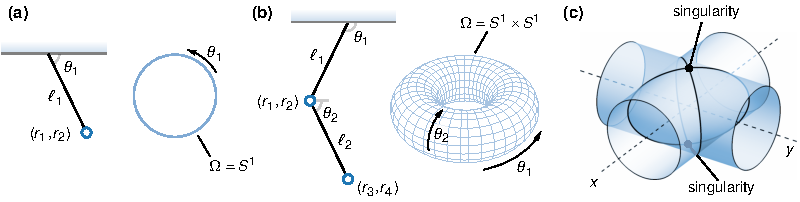
\includegraphics{intro/confspaces.pdf}
  \end{center}
  \caption{
  (a) A simple pendulum and its configuration space $\Omega = S^{1}$.
  (b) A double pendulum and its configuration space $\Omega = S^{1} \times S^{1}$.
  (c) Configuration space of a particle constrained to move on two mutually perpendicular cylinders of equal radii is the cylinders' intersection curve, which is not a smooth manifold.
  }
  \label{fig:confspaces}
  % TODO: more descriptive label.
\end{figure}

\subsection{Frameworks}

Soft, few-body systems, composed of a small number of particles or units, interacting via short-ranged forces are commonplace in soft-matter physics.
A paradigmatic example of such a system is a colloidal cluster, which is composed of a small number of colloidal particles with sizes typically ranging from 1~nm to 0.1~$\mu$m.
% TODO: figure of a colloidal cluster and cite papers in the following sentence; plagiarism issues as well.
Colloidal clusters, have been extensively studied both experimentally and theoretically, and provide fundamental insights into a host of phenomena including the formation of nucleation barriers, crystallization, glass transition, etc.
Although the particles in a colloidal cluster are held together by subtle effects of electrostatic and van der Waal forces, such details are often irrelevant if our goal is to describe the more macroscopic properties of the cluster.
To a good approximation, the interactions between the different particles are effectively described using central-force bonds connecting their centers.
Configurations of the resulting ``bond skeleton'', with each bond at its respective rest length, describe the different ground states of the cluster.
Such colloidal skeletons are an example of a mechanical framework, which is an assembly of rigid bars connecting freely-rotating joints.
Frameworks are indeed holonomically-constrained systems, not too different from the examples we have seen so far.
In case of the colloidal cluster, the configuration space of the associated framework is equivalent to the ground-state manifold of the cluster.
%
\begin{figure}
  \begin{center}
    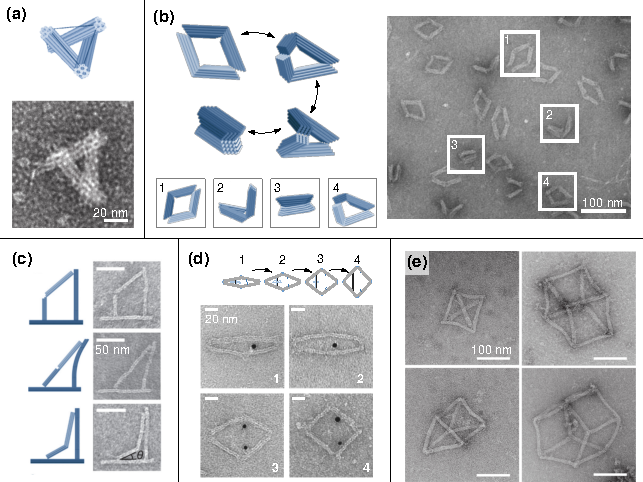
\includegraphics{intro/dna.pdf}
  \end{center}
  \caption{DNA origami has been widely used to self assemble a variety of objects at the nanoscale.
Depicted in the figure are (a) tensegrity structures \cite{liedl2010}; (b), (c) linkage-based mechanisms \cite{marras2015,zhou2015}; (d) a rhombus-shaped nanoactuator~\cite{ke2016}; and (e) self-assembled polyhedra~\cite{iinuma2014}.}
  \label{fig:dna_origami}
\end{figure}



Apart from colloidal clusters, frameworks have been extensively to understand a variety of mechanical structures found in viruses~\cite{hespenheide2004},
crystals~\cite{power2014} and minerals~\cite{kapko2011},
proteins allostery~\cite{gaspar2012}, and of course,
robots and machines~\cite{farber2008,donelan2007}.
In recent years, nanoscale frameworks made out of multihelix DNA bundles (often dubbed ``DNA origami'') have received extensive interest, with applications ranging from drug delivery~\cite{zhao2019} to self assembly~\cite{liedl2010}.
As far as more generic descriptions of thermally-driven frameworks are concerned, there has been long-standing interest in the effect of thermal fluctuations on the mechanical properties of ordered and disordered lattices~\cite{zhang2016,woodhouse2018,yan2018}, and the folding of polymerized membranes~\cite{di-francesco2000,nelson2004} and polyhedral nets~\cite{shenoy2012,dodd2018,melo2020}.
There is, therefore, an arising need to understand how thermal excitations affect the physical properties of these frameworks, but only some attempts have been made so far~\cite{kallus2017,rocklin2018}.

In practice, there is no such thing as a framework with perfect constraints, and it is always possible to violate them by paying some sort of an energy cost.
Multihelix bundles used in DNA origami, for instance, have measured stiffness in the range of 0.1--1~pN$/$nm~\cite{jung2020}.
For realistic frameworks, the configuration space $\Omega$ would then form the ground-state manifold (assuming that energy costs arise solely due to the constraints being violated).

\subsection{Free energy landscapes}

The effect of thermal fluctuations on a physical system is often represented by its free-energy landscape in terms of a set of collective variables that provide a coarse-grained description of its slowest dynamics.
In theory~\cite{go1976,echenique2011}, one can obtain the free energy of a framework by integrating out the fast modes that are transverse to its shape space, i.e., the subset of its configuration space once rigid-body motions are removed.
Doing this, however, becomes nontrivial when the framework has shape-space singularities~\cite{zlatanov2002,liu2003,donelan2007}.
For concreteness, consider the shape space of the planar four-bar linkage with freely rotating joints~\cite{grashof1883,hartenberg1964,shimamoto2005} [Fig.~\ref{fig:4bar_collage}(a)].
Though this linkage has one degree of freedom up to Euclidean motions, it has two modes of deformation, one where the angle $\theta_1 = \theta_2$ and another where $\theta_1 \ne \theta_2$, meeting at two isolated singular points $(\theta_1,\theta_2) = (0,0)$ and $(\pi,\pi)$.
One generically expects the framework to be soft at these singularities, and indeed, as we see from the blue dashed curves in Fig.~\ref{fig:4bar_collage}(b), the free energy diverges in a harmonic approximation of the elastic energy~\cite{rocklin2018}.
These divergences must be cut off by higher-order nonlinear effects, yet how this happens and to what extent remains to be understood.

In Chapters \ref{chap02} and \ref{chap03}, we develop a formalism to understand the thermal equilibration of common bar-joint frameworks that have isolated shape-space singularities.
We show that the divergent contributions to the free energy arising in the harmonic approximation to the energy are suppressed by anharmonic, quartic-order corrections.
These findings show the existence of energetic free-energy barriers between configurations near the singularities and configurations farther from the singularities.
Our results are consistent with a closely-related work~\cite{kallus2017,holmes-cerfon2017} on singular colloidal clusters, but allow for isolated singularities of the shape space.
We demonstrate our results using both the four-bar linkage as well as a flat, triangulated origami~\cite{chen2018}.
In addition to these two systems with one-dimensional configuration spaces, we also demonstrate the versatility of our methods using the five-bar linkage, which is a framework with a two-dimensional configuration space.
The analyses presented in these chapters have direct consequences in the design and employment of nanoscale frameworks in applications ranging from self-assembly~\cite{liedl2010} to drug delivery~\cite{zhao2019}, where relative thermodynamic stability of different configurations is of paramount importance.

\begin{figure}
  \begin{center}
    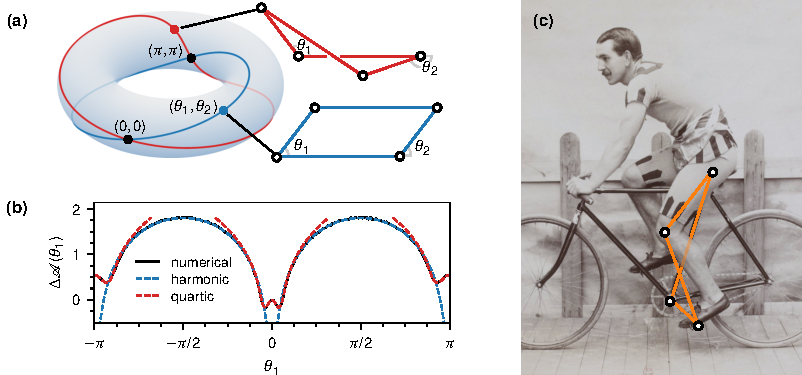
\includegraphics{intro/4bar_collage.pdf}
  \end{center}
\caption{(a) Configuration space of a four-bar linkage visualized as two intersecting curves on a torus. (b) its free energy $\mathscr{A}(\theta_{1})$ as a function of the angle $\theta_{1}$. (c) Four-bar linkage in the real world; photograph by J.~Beau, \emph{Photographie Sportive} (1898).}
  \label{fig:4bar_collage}
\end{figure}

\section{Thin structures, elastic waves, and bound states}

In the second part of this dissertation, we consider the localization of elastic waves in thin elastic structures with spatially varying curvature profiles, using a curved rod and a singly-curved shell as concrete examples.
% Previous work on related problems have largely focused on the localization of flexural waves on such structures.
% Here, using the semiclassical/WKB approximation, we show that in addition to flexural waves, extensional and shear waves also form localized, bound states around points where the absolute curvature of the structure has a minimum.
% These findings open up novel ways to fine-tune the acoustic and vibrational properties of thin elastic structures, and raise the possibility of introducing new phenomena not easily captured by effective models of flexural waves alone.

\subsection{Can one hear the shape of a shell?}

Take an ordinary hand saw used for cutting wood.
Clamp down the handle end of the saw using your feet and bend its tip using your dominant hand so that its overall shape is similar to the letter $\mathsf{S}$ (see Fig.~\ref{fig:saw}).
The saw is now a ``singing'' saw: bowing or striking it with a mallet produces a sharp, sustained sound.
But how does the saw sing, and more importantly, why does it have to be shaped like an \textsf{S}?
Although the sonorousness of the saw has been known at least since the 19th century~\cite{stuckenbruck2016}, the first scientific explanation for it was provided only in the early 90s by \citet{scott1992}.
These authors modeled the saw as a thin elastic shell with a varying curvature profile and showed that the saw's sonority is due to vibrations that get trapped around its inflection point, where the local curvature vanishes.
As trapped vibrations remain confined to the immediate vicinity of the inflection point, it reduces energy dissipation through the two ends of the saw, resulting in a sustained note.
In a very recent work, \citet{shankar2022} declared that these vibrations are topologically protected on the basis of jumps in an integral topological invariant as we move across the inflection point.

Despite the conscientious efforts of the above-mentioned authors, several critical questions remain unanswered: Do we really need an inflection point to observe trapped waves?  Is there a difference between the vibrational spectrum of one-dimensional and two-dimensional thin structures, i.e., rods vs. shells?
Is it possible to compute, even approximately, the shapes and frequencies of the vibrational modes?
What kinds of waves on thin structures get trapped?
In this dissertation, we explore these questions using a thin shell and a rod as concrete examples.

Central to understanding the trapping of waves in elastodynamic systems, such as the musical saw, is an eigenvalue problem of the form
%
\begin{equation}
  \widehat{\mathsf{D}}\psi = \omega^{2}\psi,
  \label{intro:eq:waveeq}
\end{equation}
%
which is commonplace in all mathematical sciences.
Above, $\widehat{\mathsf{D}}$ is a differential operator, $\psi$ is the wave field, and $\omega$ is the frequency of vibration.
A trapped wave is a solution $\psi$ to Eq.~\eqref{intro:eq:waveeq} satisfying the prescribed boundary conditions and decaying exponentially as we approach the physical boundaries.
In quantum-mechanical contexts, such solutions are called localized or bound states---vocabulary that we will continue to use.

In elastodynamic problems involving thin structures, the wave field $\psi$ is almost always composed of displacements---broken up into tangential and normal components---from the neutral, undeformed configuration of the structure.
The operator $\widehat{\mathsf{D}}$, the exact nature of which is model dependent, is a square matrix of spatial derivatives that act on $\psi$.
An uncurved elastic structure can support three basis wave types: extensional and shear waves, which respectively propagate by stretching and shearing the structure, and involve only the tangential components (e.g., $u$ in Fig.~\ref{fig:saw}); and flexural waves that propagate by bending the structure and involve only the normal component (e.g., $\zeta$ in Fig.~\ref{fig:saw}).
In contrast, if the structure is curved, the normal and tangential components remain coupled, and we can only speak of waves that are predominantly flexural or extensional or shear like.
It this curvature-mediated coupling between the various components that ultimately leads to the formation of bound states in curved structures.
%
\begin{figure}
  \begin{center}
    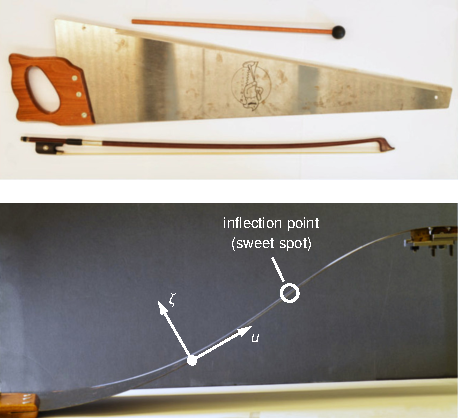
\includegraphics{intro/saw.pdf}
  \end{center}
  \caption{%
    An ordinary hand saw, when bent into the shape of the letter $\mathsf{S}$ can be played like a musical instrument using a violin's bow or a mallet.
    A sustained note is produced on bowing or hitting the saw close to its inflection point, which is called a sweet spot by saw enthusiasts.
    In most models of thin elastic structures, such as the saw here, the displacement field is broken up into a normal (e.g., $\zeta$) and tangential (e.g., $u$) component, which remain coupled if the structure is curved.
    Photographs sourced from Ref.~\cite{shankar2022}.
  }
  \label{fig:saw}
\end{figure}

\subsection{Semiclassical approximation}

The usual line of attack, when faced with an equation similar to Eq.~\eqref{intro:eq:waveeq}, is to look for plane-wave solutions of the form $\psi \sim e^{\pm i kx}$.
Such an endeavor, however, fails if the coefficients of the derivatives in $\widehat{\mathsf{D}}$ are constants, which is the case for a thin structure with a varying curvature profile.\footnote{To be clear, as the exact form of the operator $\widehat{\mathsf{D}}$ depends on the shell or rod model we choose to work with, even when the curvature is a constant, a plain-wave solution may not be applicable.}
The semiclassical approximation or the Wentzel--Kramers--Brillouin (WKB) approximation is a widely used method to obtain approximate solutions to differential equations where these coefficients are slowly varying.
In asymptotic analysis, it is usually introduced as an approximate method to find solutions to differential equations whose highest derivative is multiplied by a small parameter~\cite{bender1978}.
A paradigmatic example from physics is the time-independent Schr\"{o}dinger equation for a particle of mass $m$ in a potential $V(x)$,
%
\begin{equation}
  \left[-\frac{\hbar^{2}}{2m}\partial_{x}^{2} + V(x)\right]\psi(x) = E\psi(x),
\end{equation}
%
where the WKB method is frequently employed to find asymptotic solutions in the limit the (reduced) Planck's constant $\hbar \to 0$.
At first glance, such a limit is perplexing and makes \emph{no} physical sense as $\hbar$ is a fundamental constant, whose value is fixed by the units we choose to work in.
In reality, the limit $\hbar \to 0$ represents the situation where the value of $\hbar$ is much smaller compared to the angular momentum scale, which is often the case with macroscopic systems described by classical physics.%
\footnote{%
  This can be more clearly seen by nondimensionalizing the time-independent Schr\"{o}dinger equation by introducing an energy scale $U$ and a length scale $L$, after which it can be written as
$-\epsilon^{2}\partial_{{x}}^{2}\psi(x) + {V}(x)\psi(x) = {E}\psi(x)$,
where all quantities as well as the parameter $\epsilon = \hbar/\sqrt{2mL^{2}U}$ are now dimensionless.
As $\sqrt{2mL^{2}U}$ has dimensions of angular momentum, taking the limit $\epsilon \to 0$ is equivalent to saying that typical values of angular momentum is much larger than $\hbar$.}
It is in this context that the WKB method gets the alternative moniker of semiclassical approximation.%
%\footnote{Also known as the quasiclassical method.  In harmonic analysis, the semiclassial approximation is also called semiclassical analysis.  Some others choose to call it the eikonal method and some others call it ray approximation or ray tracing.}

Modern reformulations of the semiclassical method, based on the Weyl symbol calculus, provide unparalleled insights into the connection between classical and quantum mechanics.
Weyl calculus provides an elegant way to set up a one-to-one correspondence between differential operators (i.e., powers of $\partial_{x}$) defined on Hilbert spaces and ordinary functions defined on a position--momentum phase space.
The basic premise is that, under the Weyl transform, the momentum operator $\hat{k} = -i\partial_{x}$ gets mapped to the momentum $k$.
(For simplicity, we have suppressed factors of $\hbar$.)
Thus, after expressing the derivatives of a given differential operator $D(x, \partial_{x})$ in terms of $\hat{k}$ and its powers, the operator can be mapped to an ordinary function---called its Weyl symbol---defined on an $x$-$k$ phase space, i.e.,
%
% TODO: use tikz instead of harpoons: https:/tex.stackexchange.com/questions/312491/bumpy-uneven-arrows-in-mathtools-mhchem-etc
\begin{equation}
  \widehat{D}\left(x, \partial_{x}\right) = \widehat{D}\left(x, i\hat{k}\right) \quad\text{\small(Hilbert space)} \quad\xrightleftharpoons[\text{Wigner map}]{\text{Weyl transform}}\quad D\left(x, k\right) \quad\text{\small(phase space)}.
\end{equation}
%
The Schr\"{o}dinger operator $\widehat{H} = -\partial_{x}^{2}/2m + V(x)$, for instance, gets mapped to the classical Hamiltonian of a point particle $H(x, k) = k^{2}/2m + V(x)$.
Once the operator is in its symbol form, it can be expanded and approximated just like any other ordinary function, which provides a direct path towards obtaining asymptotic solutions to wave equations.

For matrix operators that act on multicomponent wave fields, such as the one in Eq.~\eqref{intro:eq:waveeq}, the corresponding Weyl symbol $\mathsf{D}$ is called the dispersion matrix---an ordinary matrix, whose entries are functions defined on an $x$-$k$ phase space.
The eigenvalues $\lambda(x, k)$ of the dispersion matrix serve as ray Hamiltonians of the different wave types represented by Eq.~\eqref{intro:eq:waveeq}.
This leads us to the phase space representation of waves as rays that satisfy the Hamilton's equations
%
\begin{equation}
\dot{x} = \partial_{k}\lambda(x,k)
\quad\text{and}\quad
\dot{k} = -\partial_{x}\lambda(x, k).
\end{equation}
%
The advantage provided by the semiclassical approximation cannot be overstated: we have effectively reduced the wave equation to a Hamiltonian system describing point particles, a system that is much more easier to analyze.

\subsection{Bound states in thin elastic structures}

The semiclassical approximation also provides a direct route to extract the bound state frequencies by ``quantizing'' the ray trajectories in the phase space.
As bound waves are bounded in the phase space as well, the rays corresponding to these waves appear in the form of closed orbits when visualized [see Fig.~\ref{fig:phasespace}(a)].
Each bound orbit is associated with a wave of a specific frequency $\omega$.
Additionally, the single valuedness of the wave field as we traverse the orbit requires the overall phase to be a half-integral multiple of $2\pi$.
Additional complications arise when the wave field has more than one component, which leads to a corrected Bohr--Sommerfeld-type quantization condition of the form
%
\begin{equation}
  \oint \dd{x}\,k(x) = 2\left(n + \frac{1}{2}\right)\pi - \left(\gamma_{\text{G}} + \gamma_{\text{NG}}\right).
\end{equation}
%
Here $\gamma_{\text{G}}$ and $\gamma_{\text{NG}}$ are extra phases that arise because of the multicomponent nature of the problem.
The phase $\gamma_{\text{G}}$ is a geometric phase~\cite{pancharatnam1956,berry1984}, which was very recently shown to be responsible for the topological protection of equatorial oceanic waves on the Earth's surface~\cite{venaille2023}.
That said, for the two example systems we study in this work, both the extra phases $\gamma_{\text{G}}$ and $\gamma_{\text{NG}}$ vanish.
Although one might expect this to change based on the equations we work with, this seems to be a generic result, which we expect to hold in other models of curved structures as well.

Because the extra phases vanish, the analysis becomes less cumbersome, and ultimately leads to impressive agreement between the bound-state frequencies obtained through quantization and those seen in numerical experiments.
The basic result from a combined semiclassical and numerical analysis is as follows: for the variably curved rod, which supports only extensional and flexural waves, only flexural waves form bound states; and in case of the shell, all three wave types, i.e., flexural, extensional, and shear, exhibit bound states.
For both the shell and the rod, the bound states develop around points where the absolute curvature has a minimum.
The localization of flexural waves around the inflection point of a musical saw, which is what both \citet{scott1992} and \citet{shankar2022} restricted their attention to, is a specific case of this more generic observation.
%
\begin{figure}
  \begin{center}
    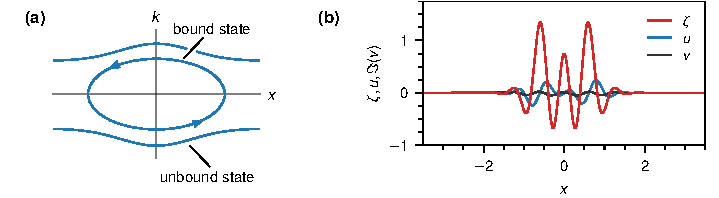
\includegraphics{figures/intro/phasespace.pdf}
  \end{center}
  \caption{(a) Phase-space representation of waves as rays, showing bound and unbound waves. (b) A predominantly flexural bound state in a uniaxially curved shell with a curvature minimum at $x = 0$ obtained by solving Eq.~\eqref{intro:eq:waveeq} numerically.
  Here $x$ is an arc-length coordinate, $\zeta$ and $u, v$ are the normal and tangential components of the displacement field, respectively; see Fig.~\ref{fig:saw} and Chapter~\ref{chap04} for more details.}
  \label{fig:phasespace}
\end{figure}
%
Many practical applications of elastic waves from acoustic cloaking to negative refraction rely on delicate aspects of wave localization.
The vast majority of these applications, however, require designer materials with intricate microstructure.
Being able to induce localization by a mere change of the material geometry is clearly advantageous.
For this reason, the results presented here lay the groundwork for the design of even simpler instruments capable of inducing wave localization.

\section{Organizational summary and other comments}

In the interest of making this dissertation more readable and self contained, I have broken up and expanded the two papers I wrote.
This dissertation is organized as follows:
In Chapter~\ref{chap02} we review basic facts about frameworks, their configuration spaces, and derive asymptotic expressions for their elastic energies.
Chapter~\ref{chap03} deals with the effect that thermal fluctuations have on these frameworks, and presents a detailed calculation of the free-energy profiles for three example frameworks.
Chapters~\ref{chap04} and~\ref{chap05} are concerned with the second problem discussed in this dissertation.
The semiclassical approximation, is reviewed in Chapter 4, with special attention paid to multicomponent wave equations.
Chapter~\ref{chap05} makes use of the semiclassical approximation to understand the formation of bound states in thin, elastic structures.
Finally, in Appendix~\ref{app:math}, we collect some helpful mathematical results that are used throughout the dissertation.

%! TEX root = thesis

\chapter{Mechanisms and Singularities}

\section{Introduction}

A \emph{mechanism} can be broadly defined as a mechanical system comprised of rigid parts that move under constraints.%
\footnote{There is some inconsistency in the definition of a mechanism.
  For instance, in some engineering contexts, a mechanism and machine are synonymous.
  On the other hand, some authors~\cite{connelly2015,rocklin2018} often call the deformation of a mechanical system allowed by its constraints a mechanism.
In this thesis, a mechanism always refers to the mechanical system considered as a whole and not its individual motions.}
A mechanism could something simple like a linear rotor to something complex like an internal-combustion engine.
A large class of mechanisms are modeled as frameworks comprising of joints connected by rigid bars.

\subsection{Four-bar linkage}

Originally analyzed by Franz Grashof~\cite[pp.~113--118]{grashof1883}.

\subsection{Fold angles}

How does one assign signs for fold angles on an origami where the faces are triangles?
Imagine that you are standing with your head pointing in the positive $z$ direction at the corner of the triangle that is opposite to the fold and facing it.
Now, keep your right feet on one of the sides and your left feet on the other.
Now when you look at the fold, if it's a mountain fold, assign it a positive sign, and if it's a valley fold, assign it a negative sign.

\subsection{Geometrical interpretation of self stress}

Suppose one can deform the mechanism while remaining in a state of self stress, then the lengths of the bars would map out a measure zero subset of the codomain.
Assume that this set can be parameterized as an $l$-dimensional surface $\Gamma$ satisfying $g(\ell) = 0$, with $l < m$.
Then during the deformation, $g(f(q)) = 0$.
%
Taking derivatives,
\begin{equation}
  \nabla g (\ell) \nabla f (q) = 0\,,
\end{equation}
%
which shows that the rows of $\nabla g(\ell)$ belong to the left kernel of $\nabla f$.
Since the rows of $\nabla g (\ell)$ span $N_{q}\Gamma$, we get the geometrical interpretation\footnote{This interpretation is due to C.~Santangelo.} that normals to the hyper surface $\Gamma$ are self stresses.
Note that this does not mean that \emph{all} self stresses belong to $N_{q}\Gamma$.
Also, this interpretation is only valid when the mechanism can be deformed while remaining in a singular state.
But in general, there could be isolated states of self stress, just like there are isolated critical points in the case of maps.
For example, consider $f: \mathbb{R}^{2} \to \mathbb{R}^{2}$ defined by $(x, y) \mapsto (1 + x^{2}, 2 + y^{2})$.
The only critical point of this map is $(0, 0)$, corresponding to a critical value $(1, 2)$.

%! TEX root = thesis.tex
% vim: ft=tex et sts=2 sw=2

\chapter{Thermal fluctuations}
\label{chap03}


% and a framework with a permanent state of self stress, which is unlike the case where it appears only at isolated singularities.

\section{Introduction}

Similar to the discussion in the previous chapter, consider a system of $N$ classical particles in $d$ dimensions.
If the position of the $i$th particle is given by the position vector $\bm{r}_{i} \in \mathbb{R}^{d}$, then the entire configuration of the system can be fully described at any moment using a configuration vector $\bm{r} \in \mathscr{R} \subseteq \mathbb{R}^{Nd}$ defined by $\bm{r} = (\bm{r}_{1}, \bm{r}_{2}, \ldots, \bm{r}_{N})$.
  Here $\mathscr{R}$ is the ambient space.%
Corresponding to $\bm{r}$ we define a momentum vector $\bm{p} = (\bm{p}_{1}, \bm{p}_{2}, \ldots, \bm{p}_{N})$, where $\bm{p}_{i}$ is the momentum of the $i$th particle.
Since there is no apriori reason for the momenta to be bounded, $\bm{p} \in \mathbb{R}^{n}$.
The microscopic state of the system at a given moment is described by the position-momentum pair $(\bm{r}, \bm{p}) \in T^{*}\mathscr{R}$, where $T^{*}\mathscr{R}$ is the cotangent bundle.
The expectation value of a macroscopic observable $\hat{\xi}$ is
%
\begin{equation}
  \braket{\hat{\xi}} = \int_{T^{*}\mathscr{R}} \dd\mu(\bm{r}, \bm{p})\, \hat{\xi}(\bm{r}, \bm{p}),
\end{equation}
%
where the Boltzmann--Gibbs measure
%
\begin{equation}
  \dd{\mu}(\bm{r}, \bm{p}) = \exp\left\{-\beta\sum_{i}\left[\frac{\bm{p}_{i}^{2}}{2m_{i}} + U(\bm{r}_{i})\right]\right\}
\end{equation}
%
Integration over $\bm{p}_{i}$ can be readily performed and the resulting multiplicative factor can be ignored for simplicity.

\subsection{Marginal densities and free energy}

The marginal probability density $\mathscr{P}(\xi)$ in terms of a \ac{cv} $\xi \in \mathbb{R}^{m}$ with $m \geq 1$ is defined as%
\footnote{This equation has been called the ``random variable transformation theorem''~\cite{gillespie1983} and can be used to prove a number of useful results in elementary probability theory; also see Ref.~\cite[Section~I.5]{kampen2007}.}
%
\begin{equation}
  \mathscr{P}(\xi) = \int \dd{\bm{r}}\, \delta[\hat{\xi}(\bm{r}) - \xi] \mathscr{P}(\bm{r}).
  \label{c03:eq:probtrans}
\end{equation}
%
To show that the above equation gives the correct marginal density, we first note that the average $\braket{\phi}$ of an observable $\phi \equiv \phi(\xi) = \phi[\hat{\xi}(\bm{r})]$ that only depends on the transformed variable $\xi$ can be computed using either the transformed density $\mathscr{P}(\xi)$ or the original density $\mathscr{P}(\bm{r})$, i.e.,
%
\begin{equation}
  \braket{\phi} = \int \dd{\tilde{\xi}}\, \phi(\tilde{\xi}) \mathscr{P}(\tilde{\xi}) = \int \dd{\bm{r}}\, \phi[\hat{\xi}(\bm{r})] \mathscr{P}(\bm{r}).
\end{equation}
%
Taking $\phi(\tilde{\xi}) = \delta(\tilde{\xi} - \xi)$ yields
%
\begin{equation}
  \int \dd{\tilde{\xi}}\, \delta(\tilde{\xi} - \xi) \mathscr{P}(\tilde{\xi}) = \mathscr{P}(\xi) = \int \dd{\bm{r}}\, \delta[\hat{\xi}(\bm{r}) - \xi] \mathscr{P}(\bm{r}).
\end{equation}
%
The free energy associated with the \ac{cv} $\xi$ is~\cite{lelievre2010}
%
\begin{equation}
  \mathscr{A}(\xi) = -\beta^{-1}\ln{\mathscr{P}(\xi)},
  \label{eq:free_energy}
\end{equation}
%
where $\beta$ is the inverse temperature.

\section{Free energy of frameworks}

Recall that the total elastic energy of a framework is of the form $U(\bm{r}) = \sum_{i=1}^{m} \phi_{i}(\ell_{i})$, where $\ell_{i}$ is the length of the $i$th bar with an energy $\phi_i(\ell_{i})$, which is assumed to have a minimum value of zero at $\ell_{i} = \bar{\ell_{i}}$, the natural length of the $i$th bar.
%
With the above form of the energy, all nontrivial ground states of a framework belong to its shape space $\Sigma$~\cite{kendall1989,mezey1993,kendall1999}, which is the set of all deformed configurations of the framework with the length of each bar equal to its natural length, once rotations and translations are removed.
% To practically identify $\Sigma$, we first switch to a Cartesian body frame attached to the framework so that all $\frac{1}{2}d(d+1)$ rigid motions are eliminated~\cite{herschbach1959,echenique2011}.
% We require $n = Nd - \frac{1}{2}d(d+1)$ coordinates to specify the state of the framework in the body frame and let $\bm{q} \in \mathbb{R}^{n}$ be its configuration vector in this frame.
% Now consider $m$ holonomic constraint functions $f_i: \mathbb{R}^{n} \to \mathbb{R},\,i=1,2,\ldots,m$, each associated with a single bar, and defined by $f_i(\bm{q}) = [\ell_i^2(\bm{q}) - \bar{\ell}_i^2]/(2\bar{\ell}_i)$.
% The $m$ scalar constraint functions can also be considered together as a single constraint map $f: \mathbb{R}^{n} \to \mathbb{R}^m$ defined by $f(\bm{q}) = [f_1(\bm{q}), f_2(\bm{q}), \ldots, f_m(\bm{q})]$.
% Then, the shape space is the zero level set $\Sigma = \left\{\bm{q} \in \mathbb{R}^{n}: f(\bm{q}) = \bm{0} \right\}$.
% In the absence of external forces, each point in $\Sigma$ is a ground-state configuration of the framework with a distinct shape.
Zero-energy shape changes constitute the slowest dynamics in a framework, so it follows that the shape coordinates $\xi$ are the most natural collective variables (CVs) for a low-dimensional description of a thermally excited framework.
%

Let us assume that the value of the chosen \ac{cv} for any configuration $\bm{q} \in \mathbb{R}^{n}$ of the framework in the body frame can be measured using the CV map $\hat{\xi}(\bm{q})$.
In the case of the four-bar linkage, for example, if we choose $\theta_{1}$ as the \ac{cv}, then $\hat{\xi}(\bm{q)}$ is the map that computes $\theta_{1}$ for any $\bm{q}$, whether or not it lies on the branches of the linkage's shape space.
For frameworks, the marginal density $\mathscr{P}(\xi)$ of the \ac{cv}, aside from factors of normalization, is
%
\begin{equation}
  \mathscr{P}(\xi) = \int_{\mathbb{R}^{n}} \dd\bm{q}\, I(\bm{q})\, \delta\left[\hat{\xi}(\bm{q}) - \xi\right] \exp\left[-\beta U(\bm{q})\right].
  \label{eq:mpd}
\end{equation}

Here $\delta[\cdot]$ is the $(n-m)$-dimensional Dirac delta function, which restricts the domain of integration to the $m$-dimensional \ac{cv} level set $\hat{\xi}^{-1}(\xi) = \left\{\bm{q} \in \mathbb{R}^{n}: \hat{\xi}(\bm{q}) = \xi\right\}$~\cite{hartmann2011}, and $I(\bm{q})$ is a Jacobian factor introduced by the change of coordinates from the lab frame to the body frame.
When $\hat{\xi}$ has full rank in $\hat{\xi}^{-1}(\xi)$, the coarea formula~\cite{lelievre2010} lets us express $\mathscr{P}(\xi)$ as an exact high-dimensional surface integral over $\hat{\xi}^{-1}(\xi)$, but evaluating it is a difficult task in practice.
Hence, we have to resort to asymptotic methods for its evaluation.

At low temperatures (i.e., large $\beta$) we can asymptotically evaluate the integral in Eq.~\eqref{eq:mpd} by expanding the energy $U(\bm{q})$ around the ground-state configurations in $\hat{\xi}^{-1}(\xi)$.
Since all ground states belong to the shape space $\Sigma$, they could be regular (i.e., nonsingular) points or singularities of $\Sigma$.
We call $\xi$ a regular value of the \ac{cv} if $\hat{\xi}^{-1}(\xi)$ does not contain singularities of $\Sigma$ and vice-versa.
For now, let us assume that $\xi$ is a regular value of the \ac{cv} and that $\hat{\xi}^{-1}(\xi)$ contains just one ground state $\bar{\bm{q}}$.
%
\begin{figure}
  \begin{center}
    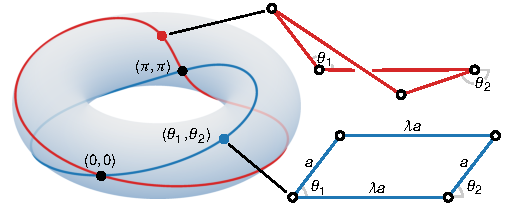
\includegraphics{frameworks/4bar_cs.pdf}
  \end{center}
  \caption{Shape space of the planar four-bar linkage visualized as two intersecting curves on a torus, each curve representing a ``branch'' of the shape space.
    The poloidal and toroidal angles along the branches correspond to the angles $\theta_1$ and $\theta_2$ of the linkage, which has two modes of deformation with $\theta_{1} = \theta_{2}$ (blue curve) and $\theta_{1} \ne \theta_{2}$ (red curve).}
  \label{fig:4bar_cs}
\end{figure}

As we remarked in the main text, the presence of the delta function restricts the domain of integration in the marginal density $\mathscr{P}(\xi)$ [Eq.~\eqref{eq:mpd}] to the \ac{cv} level set $\hat{\xi}^{-1}(\xi) = \left\{\bm{q} \in \mathbb{R}^{n}: \hat{\xi}(\bm{q}) = \xi\right\}$~\cite{hartmann2011}.
Now, since the \ac{cv} map is $\hat{\xi}: \mathbb{R}^{n} \to \mathbb{R}^{n-m}$, the CV level set $\hat{\xi}^{-1}(\xi)$ will be an $m$-dimensional manifold if $\nabla\hat{\xi}$ has full rank in $\hat{\xi}^{-1}(\xi)$.
Then, the marginal density $\mathscr{P}(\xi)$ can be written as an exact $m$-dimensional surface integral over $\hat{\xi}^{-1}(\xi)$ using the coarea formula~\cite{hartmann2007,lelievre2010,hartmann2011,diaconis2013},
%
\begin{equation}
  \mathscr{P}(\xi) = \int_{\hat{\xi}^{-1}(\xi)} \frac{\dd\Omega(\bm{q})}{\abs{\det\,\nabla\hat{\xi}(\nabla\hat{\xi})\trans}^{1/2}} I(\bm{q}) \exp{\left[-\beta U(\bm{q})\right]}.
  \label{eq:coarea}
\end{equation}
%
Here $\dd\Omega(\bm{q})$ is the surface measure on $\hat{\xi}^{-1}(\xi)$ and $\nabla\hat{\xi}$ is the $(n-m)\times n$ Jacobian matrix of $\hat{\xi}$ at $\bm{q}$.
Sometimes, Eq.~\eqref{eq:coarea} is taken to be the definition of $\mathscr{P}(\xi)$ instead of Eq.~\eqref{eq:mpd}.
This only makes sense when $\nabla\hat{\xi}$ has full rank in $\hat{\xi}^{-1}(\xi)$ so that the determinant $\det\,\nabla\hat{\xi}(\nabla\hat{\xi})\trans$ does not vanish~\cite{lelievre2010}.%
\footnote{Equation~\eqref{eq:coarea} is the arbitrary-dimensional analogue of the RHS in $\int_{\mathbb{R}} \dd{x}\, f(x)\, \delta[g(x)] = \sum_{i} f(x_{i})/\abs{g'(x_{i})}$, where $f$ and $g$ are scalar functions in $\mathbb{R}$, and $x_{i}$ are the roots of $g(x) = 0$. This is assuming $\abs{g'(x_{i})} \neq 0$, which is equivalent to the assumption that $\nabla\hat{\xi}$ has full rank in $\hat{\xi}^{-1}(\xi)$.}
Furthermore, although we have in mind an $(n-m)$-dimensional \ac{cv} $\xi$ that can be used to parameterize the branches of the shape space $\Sigma$, we do not require a parameterization at hand to use Eq.~\eqref{eq:coarea}.
For instance, in an origami the \ac{cv} could be one of its fold angles, e.g., $\rho_{1}$ in Fig.~\ref{fig:origami}, whose value can be directly computed from the coordinates of the origami.
(The map that turns the coordinates $\bm{q}$ into the fold angle is the \ac{cv} map $\hat{\xi}(\bm{q})$ for the origami.)
Hence, in theory, using this equation only requires knowledge of the energy $U(\bm{q})$, the Jacobian factor $I(\bm{q})$, and the \ac{cv} map $\hat{\xi}$.
Most importantly, Eq.~\eqref{eq:coarea} makes no reference to the shape space $\Sigma$, or its branches, or whether or not it has singularities.
However, in general, the \ac{cv} level set $\hat{\xi}^{-1}(\xi)$ is bound to be a curved high-dimensional manifold.
Hence, directly evaluating the integral in Eq.~\eqref{eq:coarea} becomes cumbersome, and we have to resort to asymptotic methods to evaluate it.

It is clear from both Eqs.~\eqref{eq:mpd} and \eqref{eq:coarea} that in the large-$\beta$ limit, contributions to the marginal density would mainly come from the neighborhoods of the ground states in the \ac{cv} level set $\hat{\xi}^{-1}(\xi)$ since the energy $U(\bm{q})$ vanishes at those points (see Fig.~\ref{fig:levelsets}).
Therefore, after asymptotically evaluating the integral in Eq.~\eqref{eq:mpd} in the neighborhood of each ground state (e.g., using Laplace's method~\cite{breitung1994}), we can then sum the results to find the asymptotic expression of the marginal density.
In the following, to simplify the presentation, we will only consider cases where the \ac{cv} level set contains just one ground state, which is either a regular point or a singularity of $\Sigma$.
As we mentioned in the main text, more general cases can then be handled by using appropriate combinations of the results we derive.

\subsection{Asymptotic PDF: regular values}
\label{sec:regular}

We first consider the case where $\xi$ is a regular value of the \ac{cv}, i.e., when the CV level set $\hat{\xi}^{-1}(\xi)$ contains only regular points of $\Sigma$.
As we remarked previously, using Eq.~\eqref{eq:coarea} to find the marginal density is difficult.
Hence, we will use a Gaussian representation of the delta function to write the marginal density as~\cite{hartmann2007a,hartmann2011}
%
\begin{equation}
  \mathscr{P}(\xi) = \lim_{\alpha\to\infty} \left(\frac{\alpha}{2\pi}\right)^{(n-m)/2} \int_{\mathbb{R}^n} \dd \bm{q}\, I(\bm{q}) \exp{\left[-\frac{1}{2}\alpha\Abs{\hat{\xi}(\bm{q}) - \xi}^2 - \beta U(\bm{q})\right]},
  \label{eq:prob_delta}
\end{equation}
%
where $\Abs{\cdot}$ is the $(n-m)$-dimensional Euclidean norm.
For $\bm{q} \in \hat{\xi}^{-1}(\xi)$, the norm $\Abs{\hat{\xi}(\bm{q}) - \xi}$ vanishes.
Similarly, for $\bm{q} \in \Sigma$, the energy $U(\bm{q})$ vanishes.
This means that in the limit $\alpha, \beta \to \infty$, contributions to the above integral would mainly come from the neighborhood of the ground state $\bar{\bm{q}} = \Sigma \cap \hat{\xi}^{-1}(\xi)$.
Hence, we can evaluate the above integral using Laplace's method after expanding the two terms in the exponent of Eq.~\eqref{eq:prob_delta} to the lowest order around $\bar{\bm{q}}$.
This gives us
%
\begin{equation}
  \mathscr{P}(\xi) \sim \lim_{\alpha\to\infty} \frac{\alpha^{-m/2}}{(2\pi)^{(n-m)/2}}I(\bar{\bm{q}})\int_{\mathbb{R}^n} \dd{\bm{q}}\, \exp\left\{-\frac{1}{2}\bm{q}\trans\left[(\nabla\hat{\xi})\trans\nabla\hat{\xi} + \alpha^{-1}\beta \mathsf{D}\right]\bm{q}\right\},
  \label{eq:prob_gaussian}
\end{equation}
%
where $\mathsf{D}$ is the dynamical matrix [see Eq.~\eqref{eq:regenergy}] and $\nabla\hat{\xi}$ is the Jacobian matrix of $\hat{\xi}$, both evaluated at $\bar{\bm{q}}$.
We have also rescaled $\bm{q} \to \alpha^{-1/2}\bm{q}$ for convenience.
%
\begin{figure}
  \begin{center}
    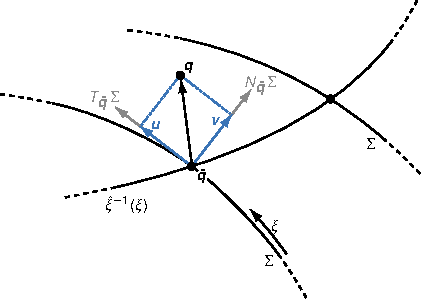
\includegraphics{frameworks/levelsets}
  \end{center}
  \caption{Cartoon illustrating the shape space $\Sigma$ parameterized by the \ac{cv} $\xi$ and the CV level set $\hat{\xi}^{-1}(\xi)$.
    In general, the sets $\Sigma$ and $\hat{\xi}^{-1}(\xi)$ could intersect at multiple points, each of which is an energy ground state.
    Tangent and normal spaces of $\Sigma$ at such a point $\bar{\bm{q}} \in \Sigma \cap \hat{\xi}^{-1}(\xi)$ are $T_{\bar{\bm{q}}}\Sigma$ and $N_{\bar{\bm{q}}}\Sigma$.}
  \label{fig:levelsets}
\end{figure}

Consider evaluating the Gaussian integral in the above equation.
Let us assume that the local parameterization of $\Sigma$ near $\bar{\bm{q}}$ in terms of the \ac{cv} is $\psi: \mathbb{R}^{n-m} \to \mathbb{R}^n$, which means that $\bar{\bm{q}} = \psi(\xi)$.
Now, the zero modes at $\bar{\bm{q}}$ belong to the tangent space $T_{\bar{\bm{q}}}\Sigma = \ker \mathsf{C}$ by definition~\cite{leimkuhler2005}.
This implies that the normal modes of the dynamical matrix, which are orthogonal to the zero modes, belong to the $m$-dimensional normal space $N_{\bar{\bm{q}}}\Sigma = (\ker\mathsf{C})^\perp$.
Since $T_{\bar{\bm{q}}}\Sigma \oplus N_{\bar{\bm{q}}}\Sigma = \mathbb{R}^n$, we can always write $\bm{q} = \bm{u} + \bm{v}$ with
$\bm{\bm{u}} \in T_{\bar{\bm{q}}}\Sigma$ and $\bm{v} \in N_{\bar{\bm{q}}}\Sigma$, for any $\bm{q} \in \mathbb{R}^n$ (see Fig.~\ref{fig:levelsets}).
As an orthonormal basis for $N_{\bar{\bm{q}}}\Sigma$, choose the normal modes $\bm{b}_1, \bm{b}_2, \ldots, \bm{b}_m \in \mathbb{R}^n$ and as the basis for $T_{\bar{\bm{q}}}\Sigma$ choose the columns of the $n\times(n-m)$ Jacobian matrix $\nabla\psi(\xi)$.%
\footnote{The normal modes need not be orthonormal if there is degeneracy in the normal frequencies.
But in such a situation, one can still pick a set of orthonormal vectors within the subspace spanned by degenerate normal modes.
With some extra steps, the derivation can also be made to work for an arbitrary basis of $N_{\bar{\bm{q}}}\Sigma$ as well.}
Therefore, we can write
%
\begin{equation}
  \bm{q} = \bm{u} + \bm{v} = (\nabla\psi)\bm{x} + \mathsf{B}\bm{y},
  \label{eq:coord_change}
\end{equation}
%
where $\mathsf{B}  = \inmat{\bm{b}_1 & \bm{b}_2 & \cdots & \bm{b}_m}$ is the change-of-basis matrix for $N_{\bar{\bm{q}}}\Sigma$.
The vectors $\bm{x} \in \mathbb{R}^{n-m}$ and $\bm{y} \in \mathbb{R}^m$ represent the components of $\bm{u}$ and $\bm{v}$ in the chosen bases.
Eq.~\eqref{eq:coord_change} suggests the coordinate change $\bm{q} \to (\bm{x}, \bm{y})$.
The quadratic form in the integral of Eq.~\eqref{eq:prob_gaussian} after such a coordinate change can be decomposed into blocks as
%
\begin{equation}
  \frac{1}{2}
  \begin{pmatrix}
    \bm{x}\trans & \bm{y}\trans
  \end{pmatrix}
  \begin{pmatrix}
    (\nabla\psi)\trans(\nabla\hat{\xi})\trans\nabla{\hat{\xi}}\nabla\psi &
    \quad(\nabla\psi)\trans(\nabla\hat{\xi})\trans\nabla\hat{\xi}\mathsf{B} \\
    \mathsf{B}\trans(\nabla\hat{\xi})\trans\nabla{\hat{\xi}}\nabla\psi &
    \quad\mathsf{B}\trans(\nabla\hat{\xi})\trans\nabla\hat{\xi}\mathsf{B} + \alpha^{-1}\beta\mathsf{D}^\perp &
  \end{pmatrix}
  \begin{pmatrix}
    \bm{x}\\
    \bm{y}
  \end{pmatrix},
  \label{eq:quadratic_form}
\end{equation}
%
where $\mathsf{D}^\perp$ is the diagonal matrix of the $m$ nonzero eigenvalues of $\mathsf{D}$.
Our assumption is that $\psi(\xi)$ is a valid parameterization of $\Sigma$ that is compatible with the \ac{cv} map $\hat{\xi}$, i.e., $\bar{\bm{q}} = \psi(\xi)$ and $\hat{\xi}(\bar{\bm{q}}) = \xi$, which means that
%
\begin{equation}
  (\hat{\xi}\circ\psi)(\xi) = \xi.
\end{equation}
%
Taking derivatives with respect to $\xi$ on both sides of the above equation we see that
%
\begin{equation}
  \nabla\hat{\xi}(\bar{\bm{q}})\nabla\psi(\xi) = \mathsf{I}_{n-m},
\end{equation}
%
where $\mathsf{I}_{n-m}$ is the $(n-m)\times(n-m)$ identity matrix.
Using this, the $n\times n$ block matrix in Eq.~\eqref{eq:quadratic_form} can be written as
%
\begin{equation}
  \begin{pmatrix}
    \mathsf{I}_{n-m} &
    \quad\nabla\hat{\xi}\mathsf{B}\\
    \mathsf{B}\trans(\nabla\hat{\xi})\trans &
    \quad\mathsf{B}\trans(\nabla\hat{\xi})\trans\nabla\hat{\xi}\mathsf{B} + \alpha^{-1}\beta\mathsf{D}^\perp
  \end{pmatrix}.
\end{equation}
%
Since $\mathsf{I}_{n-m}$ is trivially invertible, the determinant of the above matrix is
%
\begin{equation}
  \det\,\mathsf{I}_{n-m}\det\,\big[\mathsf{B} \trans(\nabla\hat{\xi})\trans\nabla\hat{\xi}\mathsf{B}  + \alpha^{-1}\beta\mathsf{D}^\perp - \mathsf{B}\trans(\nabla\hat{\xi})\trans\mathsf{I}^{-1}_{n-m}\nabla\hat{\xi}\mathsf{B}\big]
  =
  \alpha^{-m}\beta^m \det\,\mathsf{D}^\perp.
  \label{eq:determinant}
\end{equation}

Under the coordinate change $\bm{q} \to (\bm{x},\bm{y})$, the volume element $\dd{\bm{q}}$ in the integral in Eq.~\eqref{eq:prob_gaussian} acquires the factor $\sqrt{\abs{\det\,\mathsf{J}\trans\mathsf{J}}}$, where $\mathsf{J}$ is the Jacobian of the transformation.
The matrix $\mathsf{J}\trans\mathsf{J}$ can be readily cast into blocks as
%
\begin{equation}
  \mathsf{J}\trans\mathsf{J} =
  \begin{pmatrix}
    (\nabla\psi)\trans\nabla\psi & 0 \\
    0 & \mathsf{B}\trans\mathsf{B}
  \end{pmatrix}
  =
  \begin{pmatrix}
    (\nabla\psi)\trans\nabla\psi & 0 \\
    0 & \mathsf{I}_{m}
  \end{pmatrix}.
\end{equation}
%
Here $(\nabla\psi)\trans\nabla\psi$ is the metric induced by the embedding $\xi \mapsto \psi(\xi)$ and since the normal modes are orthonormal vectors, $\mathsf{B} \trans\mathsf{B}  = \mathsf{I}_m$.
Also, the off-diagonal blocks vanish since they involve inner products of the basis vectors of $T_{\bar{\bm{q}}}\Sigma$ and $N_{\bar{\bm{q}}}\Sigma$, which are orthogonal complements of each other.
This gives $\sqrt{\abs{\det\,\mathsf{J}\trans\mathsf{J}}} = \sqrt{\smash[b]{\abs{\det\, (\nabla\psi)\trans\nabla\psi}}}$, which together with Eq.~\eqref{eq:determinant} lets us evaluate the Gaussian integral in Eq.~\eqref{eq:prob_gaussian} and write
%
\begin{equation}
  \mathscr{P}(\xi) \sim I(\xi)\left(\frac{2\pi}{\beta}\right)^{m/2}
  \left|\frac{\det\,[\nabla\psi(\xi)]\trans\nabla\psi(\xi)}{\det\,\mathsf{D}^{\perp}(\xi)}\right|^{1/2}.
  \label{eq:mpd_regular}
\end{equation}
% TODO: which completes the derivation of Eq.~\eqref{eq:mpd_regular}.
The form of the above equation suggests that the nonzero eigenvalues of $\mathsf{D}$ can be naturally interpreted as being inversely proportional to the effective widths of the fluctuations along the $m$ dimensions perpendicular to $\Sigma$.
%
\begin{figure}
  \begin{center}
    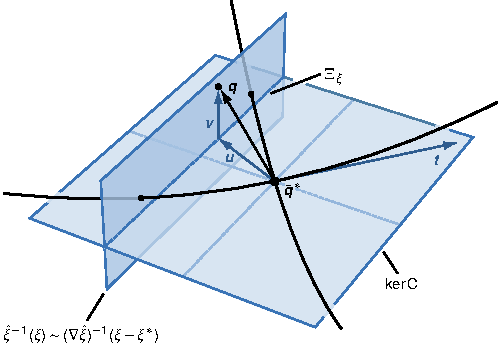
\includegraphics{frameworks/intersect.pdf}
  \end{center}
  \caption{Cartoon illustrating the geometry of the branches and the level set $(\nabla\hat{\xi})^{-1}(\xi - \xi^{*})$ of the linearized \ac{cv} map near the singularity, which is at $\bar{\bm{q}}^{*}$.
    The two ground-state configurations in the \ac{cv} level set are indicated by the intersection points of the branches with $(\nabla\hat{\xi})^{-1}(\xi - \xi^{*})$.  As $\xi \to \xi^{*}$, these ground states get infinitesimally close to each other and the framework becomes soft.
    The vector $\bm{u} \in \ker\mathsf{C}$ and the vector $\bm{v} \in (\ker\mathsf{C})^{\perp}$.
    Also indicated is a tangent vector $\bm{t}$ to a branch at the singularity.
    Here there is only one state of self stress and the delta function restricts the integral in Eq.~\eqref{eq:mpd_singular} to the line $\Xi_{\xi}$ formed by the intersection of $(\nabla\hat{\xi})^{-1}(\xi - \xi^{*})$ and $\ker\mathsf{C}$.
  }
  \label{fig:intersect}
\end{figure}

\subsection{Asymptotic PDF: singular values}
\label{sec:singular}

Equation~\eqref{eq:mpd_regular} breaks down as we approach a singularity along $\Sigma$ since the lowest $s$ nonzero eigenvalues of $\mathsf{D}$ become very small and tend to zero, and we need an alternative method to find the marginal densities.
At a singular point of $\Sigma$ with $s$ self stresses, the number of zero modes increases by $s$, which means that now there are only $m-s$ normal modes.
A cartoon of the situation is depicted in Fig.~\ref{fig:intersect}, which shows two branches of a one-dimensional shape space $\Sigma$ intersecting at a singularity $\bar{\bm{q}}^{*}$, where the \ac{cv} has the value $\xi^{*}$.
Because of the additional self stress, the subspace of zero modes $\ker\mathsf{C}$ is now a plane, which is tangent to both the branches at the singularity.
%Since $\Sigma$ is not a smooth manifold at $\bar{\bm{q}}^{*}$, one cannot also define a tangent space at $\bar{\bm{q}}^{*}$.

How should one proceed in such a situation?
At first glance, one might think that all that is required is to replace the harmonic energy in the previous derivation with the quartic energy expansion [Eq.~\eqref{eq:energy_singular}].
This cannot be correct as Eq.~\eqref{eq:energy_singular} is only valid when the expansion is around the singularity, and our goal here is to find $\mathscr{P}(\xi)$ not just for the singular \ac{cv} value $\xi^{*}$, but for all $\xi \to \xi^{*}$.
When $\xi$ is close to $\xi^{*}$, the ground-state configurations in $\hat{\xi}^{-1}(\xi)$ are all regular points of $\Sigma$ that do not have any singular zero modes.
However, at these configurations, the framework also becomes very soft in certain directions due to the presence of the nearby singularity, causing the harmonic approximation to break down.
A possible strategy could then be to expand the energy to both harmonic and quartic order along these special soft modes, i.e., those that will ultimately become a zero mode at the singularity as we move along $\Sigma$.
Apart from the complexity of such an expansion, this raises another issue: how should one perform Laplace asymptotics around the ground states in $\hat{\xi}^{-1}(\xi)$?
When $\xi$ is close to $\xi^{*}$, the ground states in $\hat{\xi}^{-1}(\xi)$ get infinitesimally close to each other, as do the branches (see Fig.~\ref{fig:intersect}).
Hence, on doing Laplace asymptotics around each of these ground states and on extending the integration domain to infinity, we would be adding contributions to the marginal density from the same region more than once.
In this sense, the contributions from the branches are not separable in the vicinity of the singularity.

From the above discussion, it should be evident that the approach we used in deriving the harmonic marginal density [Eq.~\eqref{eq:mpd_regular}] will not work for finding an asymptotic expression for $\mathscr{P}(\xi)$ for $\xi \to \xi^{*}$.
The only possibility then is to rely on Eq.~\eqref{eq:coarea}, which expresses $\mathscr{P}(\xi)$ as an exact integral over the \ac{cv} level set $\hat{\xi}^{-1}(\xi)$.
Note again that Eq.~\eqref{eq:coarea} makes no reference to the shape space $\Sigma$ as such, enabling us to side step the issues described above.
This however, comes at the expense of having to do a higher-dimensional integral over $\hat{\xi}^{-1}(\xi)$.
The next strategy is to make physically valid assumptions that can be used to dimensionally reduce this integral.

% To simplify the evaluation, we make two assumptions: (i) for points close to $\bar{\bm{q}}^{*}$, the \ac{cv} map $\hat{\xi}$ can be approximated by its Taylor expansion around $\bar{\bm{q}}^{*}$: $\hat{\xi} = \xi^{*} + (\nabla\hat{\xi})\bm{q} + \mathcal{O}(\Abs{\bm{q}}^{2})$, with $\nabla\hat{\xi}$ being the Jacobian matrix of $\hat{\xi}$ at $\bar{\bm{q}}^{*}$; (ii) fast modes that belong to $(\ker\mathsf{C})^{\perp}$ do not change the value of the CV to linear order at $\bar{\bm{q}}^{*}$, i.e., $(\nabla\hat{\xi})\bm{v} = \bm{0}$.
% Assumption (i) linearizes the \ac{cv} map and turns its level sets near the singularity into hyperplanes, simplifying the evaluation of Eq.~\eqref{eq:mpd}.
% Although assumption (ii) is stringent on the shape coordinate we use as the \ac{cv}, it is true for most reasonable choices and a good CV should mainly be sensitive to the slow modes~\cite{tiwary2016}.
% This makes it possible to use the quartic energy expansion and integrate over the fast modes.

The first such assumption we make is that the \ac{cv} map can be approximated by its Taylor expansion $\hat{\xi} = \xi^{*} + (\nabla\hat{\xi})\bm{q} + \mathcal{O}(\Abs{\bm{q}}^2)$ around the singularity $\bar{\bm{q}}^{*}$ for points close to $\bar{\bm{q}}^{*}$.
with $\nabla\hat{\xi}$ being the Jacobian matrix of $\hat{\xi}$ at $\bar{\bm{q}}^{*}$.
This linearizes the \ac{cv} map and turns its level sets $(\nabla\hat{\xi})^{-1}(\xi - \xi^{*}) = \{\bm{u} \in \mathbb{R}^{n}: \xi^{*} + (\nabla\hat{\xi})\bm{u} = \xi\}$ near the singularity into hyperplanes (see Fig.~\ref{fig:intersect}).
Since this hyperplane is considerably easier to parameterize in comparison to the actual \ac{cv} level set $\hat{\xi}^{-1}(\xi)$, this makes the evaluation of $\mathscr{P}(\xi)$ as a surface integral using Eq.~\eqref{eq:coarea} less difficult.
The second assumption is that the fast modes $\bm{v} \in (\ker\mathsf{C})^{\perp}$ are such that they do not change the value of the \ac{cv} to linear order at the singularity, i.e., $(\nabla\hat{\xi})\bm{v} = \bm{0}$.
This enables us to write $\bm{q} = \bm{u} + \bm{v}$, with $\bm{u} \in \ker\mathsf{C}$ and $\bm{v} \in (\ker\mathsf{C})^\perp$, and use the lowest-order approximation of the energy near the singularity [Eq.~\eqref{eq:energy_singular}] to get\footnote{The Jacobian factor introduced by the transformation $\bm{q} \to (\bm{u}, \bm{v})$ is unity if we pick orthonormal bases for $\ker\mathsf{C}$ and $(\ker\mathsf{C})^{\perp}$.}
%
\begin{equation}
  \hspace{-0.5em}
  \begin{aligned}
    \mathscr{P}(\xi) &= \int \dd\bm{q}\, I(\bm{q})\,\delta\left[\hat{\xi}(\bm{q}) - \xi\right] \exp\left[-\beta U(\bm{q})\right]\\
                                 &\sim I(\xi^{*}) \int_{\ker\mathsf{C}} \dd\bm{u}\, \delta\left[(\nabla\hat{\xi})\bm{u} - (\xi - \xi^{*})\right] \int_{(\ker\mathsf{C})^{\perp}} \dd\bm{v}\,  \exp\left\{-\frac{1}{2}\beta\kappa[\mathsf{C}\bm{v} + \bm{w}(\bm{u})]\trans[\mathsf{C}\bm{v} + \bm{w}(\bm{u})]\right\},
  \end{aligned}
\end{equation}
%
where we have used $(\nabla\hat{\xi})(\bm{u} + \bm{v}) = (\nabla\hat{\xi})\bm{u}$.
As we can see from the above equation, the second assumption has allowed us to separate the contributions to $\mathscr{P}(\xi)$ from the fast vibrational modes in $(\ker\mathsf{C})^{\perp}$ and the zero modes in $\ker\mathsf{C}$.
As before, we choose the $m - s$ normal modes as the basis for $(\ker\mathsf{C})^{\perp}$ and write $\bm{v} = \mathsf{B}\bm{y}$, with $\mathsf{B}$ being the change-of-basis matrix and $\bm{y} \in \mathbb{R}^{m-s}$ representing the components of $\bm{v}$ in the chosen basis.
This turns the integral over $(\ker\mathsf{C})^{\perp}$ into an $(m-s)$-dimensional Gaussian integral over $\bm{y}$, which after a straightforward integration yields
%
\begin{equation}
  \hspace{-0.5em}
  \begin{aligned}
    \mathscr{P}(\xi) &\sim I(\xi^{*}) \int_{\ker\mathsf{C}} \dd\bm{u}\, \delta\left[(\nabla\hat{\xi})\bm{u} - (\xi - \xi^{*})\right] \int_{\mathbb{R}^{m-s}} \dd\bm{y}\, \exp\left\{-\frac{1}{2}\beta\kappa[\mathsf{C}\mathsf{B}\bm{y} + \bm{w}(\bm{u})]\trans[\mathsf{C}\mathsf{B}\bm{y} + \bm{w}(\bm{u})]\right\}\\
                                             &= \frac{I(\xi^{*})}{\left|\det\, \mathsf{D}^\perp\right|^{1/2}} \left(\frac{2\pi}{\beta}\right)^{(m-s)/2} \int_{\ker\mathsf{C}} \dd\bm{u}\, \delta\left[(\nabla\hat{\xi})\bm{u} - (\xi - \xi^{*})\right] \exp\left[-\frac{1}{2}\beta\kappa \bm{w}(\bm{u})\trans\Pi \bm{w}(\bm{u})\right],
  \end{aligned}
  \label{eq:mpd_gaussian}
\end{equation}
%
where $\mathsf{D}^\perp$ is the diagonal matrix of the $m - s$ nonzero eigenvalues of $\mathsf{D}$ at the singularity and
%
\begin{equation}
  \Pi = \mathsf{I}_{m} - \mathsf{C}\mathsf{B} (\mathsf{B} ^\mathsf{T}\mathsf{C}^\mathsf{T}\mathsf{C}\mathsf{B} )^{-1}\mathsf{B} ^\mathsf{T}\mathsf{C}^\mathsf{T}
\end{equation}
%
is a projection operator%
\footnote{This operator may be compared with a similar projection operator that appears in the theory of polymerized membranes, once the in-plane components of the elastic free energy (i.e., the fast modes) are integrated out; see, e.g., Eqs.~(6)--(8) of Ref.~\cite{nelson1987}.}
that projects $\bm{w}(\bm{u})$ to the cokernel of $\mathsf{C}\mathsf{B}$ (i.e., to $\ker\mathsf{B}\trans\mathsf{C}\trans$).
Note that this operator would trivially have been the identity matrix if it were not for the cross term $\bm{w}(\bm{u})\trans\mathsf{K}\mathsf{C}\bm{v}$ in the energy expansion [Eq.~\eqref{eq:energy_singular}] that couples the fast modes and the zero modes.
Since the cokernel of $\mathsf{CB}$ is identical to the cokernel of $\mathsf{C}$, it is spanned by an orthonormal basis of self stresses $\bm{\sigma}$, and one can write the action of $\Pi$ on $\bm{w}(\bm{u})$ as
%
\begin{equation}
  \Pi \bm{w}(\bm{u)} = \sum_{\bm{\sigma}} \bm{\sigma}[\bm{\sigma}\cdot\bm{w}(\bm{u})].
  \label{eq:mpd_proj}
\end{equation}
%
Using this in Eq.~\eqref{eq:mpd_gaussian} and after a straightforward application of the coarea formula [Eq.~\eqref{eq:coarea}] we find to the lowest order, for $\xi \to \xi^{*}$,
%
\begin{equation}
  \begin{aligned}
    \mathscr{P}(\xi) &\sim \frac{I(\xi^{*})}{\left|\det\, \mathsf{D}^\perp\right|^{1/2}} \left(\frac{2\pi}{\beta}\right)^{(m-s)/2} \int_{\ker\mathsf{C}} \dd\bm{u}\, \delta\left[(\nabla\hat{\xi})\bm{u} - (\xi - \xi^{*})\right] \exp\left\{-\frac{1}{2}\beta\kappa\sum_{\bm{\sigma}}[\bm{\sigma}\cdot \bm{w}(\bm{u})]^2\right\}\\
                                 &= \frac{I({\xi}^{*})}{\left|\det\, \mathsf{D}^\perp \det\, \nabla\hat{\xi}(\nabla\hat{\xi})\trans\right|^{1/2}}  \left(\frac{2\pi}{\beta}\right)^{(m-s)/2} \int_{\Xi_{\xi}} \dd\Omega(\bm{u})\, \exp\left\{-\frac{1}{2}\beta\kappa\sum_{\bm{\sigma}}[\bm{\sigma}\cdot\bm{w}(\bm{u})]^2\right\}.
  \end{aligned}
  \label{eq:mpd_singular}
\end{equation}
%
Above, the integration domain $\Xi_{\xi} = (\nabla\hat{\xi})^{-1}(\xi - \xi^{*}) \cap \ker\mathsf{C}$, is a hyperplane of $(n - m + s) - (n - m) = s$ dimensions and $\dd\Omega(\bm{u})$ is the surface measure on $\Xi_{\xi}$.
After choosing a convenient parameterization for $\Xi_{\xi}$ in terms of the components of $\bm{u}$ in some basis of $\ker\mathsf{C}$, Eq.~\eqref{eq:mpd_singular} becomes an $s$-dimensional integral involving the exponential of a quartic polynomial, which should converge if $\Sigma_{\bm{\sigma}} [\bm{\sigma}\cdot\bm{w}(\bm{u)}]^2$ does not identically vanish in some region of $\Xi_{\xi}$ that extends to infinity (see below for an extended discussion on this).
This completes the derivation of Eq.~\eqref{eq:mpd_singular}.
In deriving Eq.~\eqref{eq:mpd_singular}, unlike in the derivation of Eq.~\eqref{eq:mpd_regular}, we have not looked at contributions to $\mathscr{P}(\xi)$ from the ground states on each branch of $\Sigma$ individually.
Hence, Eq.~\eqref{eq:mpd_singular} represents the collective contribution to the marginal density from all the branches that intersect to form the singularity at $\bar{\bm{q}}^{*}$.

\subsubsection*{Convergence of the integral in \texorpdfstring{Eq.~\eqref{eq:mpd_singular}}{Eq. (5)}}
\label{sec:convergence}

Before discussing the conditions that are required for the integral in Eq.~\eqref{eq:mpd_singular} to converge, we digress slightly and discuss second-order rigidity, a frequently invoked notion in rigidity theory~\cite{connelly1994,connelly1996}.
In the notation that we have been using, a bar-joint framework is considered to be second-order rigid if there are no vector pairs $(\bm{u}, \bm{v})$ with $\bm{u} \in \ker\mathsf{C}$ and $\bm{v} \in (\ker\mathsf{C})^{\perp}$ such that\footnote{Note that this equation is nothing but the Taylor expansion of the constraint map $f$ to the lowest order in $\bm{u}$ and $\bm{v}$.}
%
\begin{equation}
  \mathsf{C}\bm{v} + \bm{w}(\bm{u}) = \bm{0}.
\end{equation}
%
For a singular configuration of the framework that supports nonzero self stresses $\bm{\sigma}$, second-order rigidity is equivalent to saying that there is no zero mode $\bm{u} \in \ker\mathsf{C}$ such that\footnote{See, e.g., Corollary 5.2.2 of Ref.~\cite{connelly1996} or Corollaries 4.15--4.17 of Ref.~\cite{williams2003}.}
%
\begin{equation}
  \bm{\sigma}\cdot\bm{w}(\bm{u}) = 0,\label{eq:2ndorder}
\end{equation}
%
for all $\bm{\sigma} \in \ker\mathsf{C}\trans$.
A well-known result is that a bar-joint framework is rigid to all orders if it is second-order rigid~\cite{connelly1996}.

Clearly, a framework is not rigid (to any order) by definition and all tangents to the branches of the shape space $\Sigma$ at a singularity $\bar{\bm{q}}^{*}$ satisfy Eq.~\eqref{eq:2ndorder}.
Even though one can speak of tangent vectors to the branches of $\Sigma$ at $\bar{\bm{q}}^{*}$, the shape space $\Sigma$ itself ceases to be a smooth manifold at $\bar{\bm{q}}^{*}$.
Hence, there is no well-defined tangent space at $\bar{\bm{q}}^{*}$ and it is common practice to consider instead the solution space of Eq.~\eqref{eq:2ndorder},
%
\begin{equation}
  \mathscr{T} = \left\{\bm{t} \in \ker\mathsf{C} : \bm{\sigma}\cdot \bm{w}(\bm{t}) = 0 \text{ for all } \bm{\sigma} \in \ker\mathsf{C}\trans \right\},
  \label{eq:tangentcone}
\end{equation}
%
which is the set of zero modes that preserve the constraints to second-order~\cite{chen2018}.
For this reason, $\mathscr{T}$ is often called the second-order tangent cone.\footnote{See, e.g., Section 4.2 of Ref.~\cite{wu2020}; also see the related discussions in Refs.~\cite{muller2017,muller2019,lopez-custodio2020}.
Tangent cones themselves were originally introduced by \citet{whitney1965} to study tangents to analytic varieties.}
Even though the tangents to the branches of $\Sigma$ belong to $\mathscr{T}$, in general, there could be vectors in $\mathscr{T}$ that are not tangents.
In such situations, the tangents cannot be resolved by considering the second-order tangent cone alone and higher-order analysis is necessary~\cite{muller2017,lopez-custodio2020}.
To simplify things, from here on we assume that the tangents can be resolved at second order, i.e., every element of $\mathscr{T}$ is a tangent to the branches of the shape space $\Sigma$ at the singularity.
For instance, in the cartoon in Fig.~\ref{fig:intersect}, $\mathscr{T}$ would be the union of the two tangents at the singularity.

Now, the integral that defines $\mathscr{P}(\xi)$ also includes a delta function $\delta[\hat{\xi}(\bm{q}) - \xi]$.
After linearizing the \ac{cv} map $\hat{\xi}$ around the singularity and integrating out the fast modes, the domain of integration in Eq.~\eqref{eq:mpd_singular} becomes the hyperplane $\Xi_{\xi} = \ker\mathsf{C} \cap (\nabla\hat{\xi})^{-1}(\xi - \xi^{*})$.
At a singularity with $s$ self stresses $\bm{\sigma}_{1}, \bm{\sigma}_{2}, \ldots, \bm{\sigma}_{s}$, consider the map $g: \ker\mathsf{C} \to \mathbb{R}^{n - m + s}$ defined by $g(\bm{u}) = [(\nabla\hat{\xi})\bm{u} - (\xi - \xi^{*}), \bm{\sigma}_{1}\cdot \bm{w}(\bm{u}), \bm{\sigma}_{2}\cdot \bm{w}(\bm{u}), \ldots, \bm{\sigma}_{s}\cdot \bm{w}(\bm{u})]$.
In a basis of $\ker\mathsf{C}$, the equation $g(\bm{u}) = \bm{0}$ defines an exactly determined system of equations in $n-m+s$ unknowns, whose solutions (if they exist) are tangents that belong to $\Xi_{\xi}$.
If this equation has isolated roots, then the term $\sum_{\bm{\sigma}} [\bm{\sigma}\cdot\bm{w}(\bm{u})]^{2}$ in the exponential of Eq.~\eqref{eq:mpd_singular} is zero only for a discrete set of tangent vectors in $\Xi_{\xi}$ and is positive everywhere else, making the integral convergent.
(In Fig.~\ref{fig:intersect}, this discrete set is composed of the tangents to the two branches, which when extended intersect the line $\Xi_{\xi}$, which is the domain of integration.)
A necessary condition for the equation $g(\bm{u}) = \bm{0}$ to have isolated roots in $\Xi_{\xi}$ is that $(\nabla\hat{\xi})\bm{t} \neq \bm{0}$ for all $\bm{t} \in \mathscr{T}$.
Given how $g(\bm{u})$ is a system of $n - m$ linear and $s$ quadratic equations, a stronger general condition that ensures this eludes us at present.
On the other hand, if there is a tangent $\bm{t}$ such that $(\nabla\hat{\xi})\bm{t} = \bm{0}$, the integral diverges.
Such cases are pathological and indicate a poor \ac{cv} choice.
After all, if $\bm{t}$ is a tangent to $\Sigma$, then it is a slow mode that corresponds to a shape change in the framework, and one would definitely want the value of the \ac{cv} to change along it.

To conclude, the convergence of Eq.~\eqref{eq:mpd_singular} relies on the term $\sum_{\bm{\sigma}}[\bm{\sigma}\cdot\bm{w}(\bm{u})]^{2}$ in the exponential vanishing only for a finite number of isolated points in the integration domain $\Xi_{\xi}$.
Two necessary conditions required for this are: (i) tangents to the branches of the shape space at the singularity can be resolved at second order and form the solution space $\mathscr{T}$ of Eq.~\eqref{eq:2ndorder}, and (ii) the \ac{cv} map is such that $(\nabla\hat{\xi})\bm{t} \neq 0$ for all $\bm{t} \in \mathscr{T}$.

\subsubsection*{Scaling of the marginal density}
\label{sec:scaling}

To see how the marginal density $\mathscr{P}(\xi^{*})$ at a singular value $\xi^{*}$ scales with $\beta$ and $\kappa$, we first choose a basis for $\ker\mathsf{C}$ so that $\bm{u} = \mathsf{A}\bm{x}$, where $\bm{x} \in \mathbb{R}^{n-m+s}$ represents the components of $\bm{u}$ in the chosen basis and $\mathsf{A}$ is the associated change-of-basis matrix.
Now, the $s$-dimensional hyperplane $\Xi_{\xi}$ formed by the intersection of the linearized \ac{cv} level set and $\ker\mathsf{C}$ is defined by $\nabla\hat{\xi}\mathsf{A}\bm{x} = \bm{0}$, which is a set of $n-m$ homogeneous linear equations in $n-m+s$ variables.
Without loss of generality, let us assume that we can solve these equations to obtain the last $n - m$ components of $\bm{x}$ in terms of its first $s$ components $\tilde{\bm{x}} = (x_{1}, x_{2}, \ldots, x_{s})$.
This enables us to parameterize the hyperplane $\Xi_{\xi}$ using $\tilde{\bm{x}}$.
As each component of the vector $\bm{w}(\bm{u})$ is a quadratic form in $\bm{x}$, after the elimination step, the term $\sum_{\bm{\sigma}}[\bm{\sigma}\cdot\bm{w}(\bm{u})]^{2}$ in the exponential of Eq.~\eqref{eq:mpd_singular} becomes a homogeneous quartic polynomial $\widetilde{U}(\tilde{\bm{x}})$.
A rescaling of the components $\tilde{\bm{x}} \to (\beta\kappa)^{-1/4}\tilde{\bm{x}}$, changes the surface measure from $\dd\Omega(\tilde{\bm{x}}) \to (\beta\kappa)^{-s/4}\dd\Omega(\tilde{\bm{x}})$ and turns $\widetilde{U}(\tilde{\bm{x}}) \to (\beta\kappa)^{-1}\widetilde{U}(\tilde{\bm{x}})$, yielding
%
\begin{equation}
  \mathscr{P}(\xi^{*}) \sim \frac{I({\xi}^{*})}{\left|\kappa^{s/2}\det\,\mathsf{D}^\perp \det\, \nabla\hat{\xi}(\nabla\hat{\xi})\trans\right|^{1/2}}  \left(\frac{2\pi}{\beta}\right)^{m/2 - s/4} \int_{\Xi_{\xi}} \dd\Omega(\tilde{\bm{x}})\, \exp\left[-\frac{1}{2}\widetilde{U}(\tilde{\bm{x}})\right].
  \label{eq:scaling}
\end{equation}
%
Clearly, the above integral is purely geometric in nature and all $\beta$ dependence has been extracted
Finally, noting that $\det\,\mathsf{D}^{\perp} \sim \kappa^{m - s}$ we see that the marginal density $\mathscr{P}(\xi^{*}) \sim (\beta\kappa)^{-m/2 + s/4}$.
It should be emphasized that we can only do this analysis for $\xi = \xi^{*}$.
For other values of $\xi$ close to $\xi^{*}$, the hyperplane $\Xi_{\xi}$ is defined by the inhomogeneous equation $\nabla\hat{\xi}\mathsf{A}\bm{x} = \xi - \xi^{*}$, which makes $\widetilde{U}(\tilde{\bm{x}})$ a similarly inhomogeneous quartic polynomial, making a rescaling argument impossible.

The marginal density for regular values of the \ac{cv}, which scales like $\mathscr{P}(\xi) \sim (\beta\kappa)^{-m/2}$ [Eq.~\eqref{eq:mpd_regular}], is always subdominant to the marginal density at a singular value $\xi^{*}$, which scales like $\mathscr{P}(\xi^{*}) \sim (\beta\kappa)^{-m/2 + s/4}$ for $s > 0$.
Hence, we see that the softening of the framework at a singularity causes an energetic free-energy barrier to develop between regular and singular values of the \ac{cv}, with a temperature/stiffness dependence $\sim \ln \beta\kappa$.
In comparison, the free-energy barriers between singular values of the \ac{cv} are independent of $\beta$ and $\kappa$, and depend only on geometric parameters if the corresponding configurations have the same number of self stresses $s$.
Although this might lead us to conclude that such barriers are entropic in origin, note that there would be energetic barriers along most realizable transition paths separating these configurations.

The stark difference in the asymptotic scaling of $\mathscr{P}(\xi)$ at a singular value $\xi = \xi^{*}$ and for values farther from it shows that the true scaling and behavior of $\mathscr{P}(\xi)$ for intermediate values of $\xi$ is nontrivial.
A natural question is then: for what values of $\xi$ would the harmonic and quartic approximations capture the true behavior of $\mathscr{P}(\xi)$?
Equation~\eqref{eq:mpd_regular}, derived using the harmonic approximation and a direct application of Laplace's method, is only accurate so long as the lowest nonzero eigenvalue $\omega_{\text{min}}(\xi)$ of the dynamical matrix $\mathsf{D}$ is such that $\beta\omega_{\text{min}}(\xi)$ is very large.
This is also what causes it to break down as we approach a singularity, near which $\omega_{\text{min}}(\xi)$ monotonically\footnote{For one-dimensional shape spaces, using Rayleigh--Schr\"{o}dinger perturbation theory~\cite{dirac1958} and considering the dynamical matrix at the singularity as the ``unperturbed Hamiltonian'', it can be shown that $\omega_{\text{min}} \sim (\xi - \xi^{*})^{2}$ for $\xi \to \xi^{*}$.} decreases to zero as $\xi \to \xi^{*}$.
This also implies that as $\beta$ becomes larger, the harmonic approximation starts capturing the true behavior of the marginal density for a larger range of $\xi$ values.
For very large $\beta$, the range of validity of the quartic approximation is also bound to increase as the errors in the approximation become small.
This means that, for large $\beta$, we expect to see some amount of overlap in the marginal density estimates using Eqs.~\eqref{eq:mpd_regular} and \eqref{eq:mpd_singular} as evidenced by the free-energy curves in Figs.~\ref{fig:4bar_free} and \ref{fig:origami}(c).
We expect the exact nature of the overlap to be problem specific with a strong dependence on $\beta$ and we leave a more thorough analysis for future work.

% TODO: Reduce line break; there has to be a line break though, because this paragraph is a break in the thought flow.
\phantom{}\\
We now use our formalism to find the free-energy profiles of two example frameworks with one-dimensional shape spaces with isolated singularities and compare them with results from Monte Carlo simulations.
We will also use our formalism to analyze the five-bar linkage, a framework with a two-dimensional shape space.
Motivated by typical DNA origami structures that have lengths in the range of a few hundred nanometers with stiffness in the range 0.1--1~pN$/$nm~\cite{jung2020}, we choose a nondimensional inverse temperature of $\beta = 10^{4}$ and use a potential of the form $\phi_{i}(\ell_{i}) = (\ell_{i}^{2} - \bar{\ell}_{i}^{2})^{2}/(8\bar{\ell}_{i}^{2})$ so that $\phi_{i}''(\bar{\ell}_{i}) = \kappa = 1$.
Further details on the simulations are given in Appendix~\ref{sec:numerics}.

%If $\bm{q}$ is a point near $\bar{\bm{q}}$, after setting $\bm{q} \to \bar{\bm{q}} + \bm{q}$, we expand the energy to the lowest order around $\bar{\bm{q}}$ and find the harmonic energy $U \approx \frac{1}{2}\bm{q}\trans\mathsf{C}\trans\mathsf{K}\mathsf{C}\bm{q} = \frac{1}{2}\bm{q}\trans\mathsf{D}\bm{q}$.
%Here $\mathsf{D} = \mathsf{C}\trans\mathsf{K}\mathsf{C}$ is the dynamical matrix evaluated at $\bar{\bm{q}}$~\cite{lubensky2015} (assuming joints of unit mass) and $\mathsf{K}$ is the diagonal matrix of bar stiffnesses $\phi_{i}''(\bar{\ell}_{i})$, which we set equal to $\kappa$ for all bars for simplicity.
%See the Supplemental Material (SM) for details.
%Since $\bar{\bm{q}}$ is a regular point of $\Sigma$, $\mathsf{C}$ has full rank, and $\mathsf{D}$ has $n-m$ independent zero modes that belong to $\ker\mathsf{C} = \left\{\bm{u} \in \mathbb{R}^{n}: \mathsf{C}\bm{u} = \bm{0}\right\}$~\cite{lubensky2015}.
%These zero modes are all tangent to $\Sigma$ and represent a degree of freedom~\cite{leimkuhler2005}.
%Hence, to asymptotically evaluate Eq.~\eqref{eq:mpd} in the neighborhood of a regular point, we can safely use the harmonic approximation since any divergence~\cite{schwarz1979,ellis1981,rocklin2018} due to these zero modes is regularized by the delta function, which suppresses all contributions to the integral that are tangent to $\Sigma$~\cite{ramond1997}.
%Then, the asymptotic marginal density for a regular value $\xi$ of the \ac{cv} is (SM)
%%
%\begin{equation}
%  \mathscr{P}(\xi) \sim I(\xi)\left(\frac{2\pi}{\beta}\right)^{m/2}
%  \left|\frac{\det\,[\nabla\psi(\xi)]\trans\nabla\psi(\xi)}{\det\,\mathsf{D}^{\perp}(\xi)}\right|^{1/2}.
%  \label{eq:mpd_regular}
%\end{equation}
%%
%Here $\psi: \mathbb{R}^{n-m} \to \mathbb{R}^{n}$ is a parameterization of $\Sigma$ near $\bar{\bm{q}} \in \Sigma$ in terms of the \ac{cv} $\xi$, and compatible with the CV map, such that $\bar{\bm{q}} = \psi(\xi)$ and $\hat{\xi}(\bar{\bm{q}}) = \xi$.
%Also, $\det\,(\nabla\psi)\trans\nabla\psi$ is the determinant of the induced metric on $\Sigma$ and $\mathsf{D}^{\perp}$ is the diagonal matrix of the $m$ nonzero eigenvalues of $\mathsf{D}$ at $\bar{\bm{q}}$.

%Now, consider the situation at a shape-space singularity, where $\mathsf{C}$ has rank deficiency.
%At such a point, using the Maxwell--Calladine count~\cite{maxwell1864,calladine1978}, we find that the number of zero modes increases to $n - m + s$, where $s$ is the number of independent self stresses $\bm{\sigma} \in \ker\mathsf{C}\trans$---each self stress being a set of bar tensions that leave the framework in equilibrium~\cite{lubensky2015}.
%The zero modes at a singularity are not all tangent to $\Sigma$, which means that the delta function in Eq.~\eqref{eq:mpd} fails to suppress the divergences due to these zero modes when the harmonic approximation is used.
%Furthermore, as one approaches the singularity along $\Sigma$, the lowest $s$ nonzero eigenvalues of the dynamical matrix $\mathsf{D}$ become small leading to an effective softening of the framework.
%This causes Eq.~\eqref{eq:mpd_regular} to break down even for regular ground states in the vicinity of the singularity.
%For instance, for the four-bar linkage, using Eq.~\eqref{eq:mpd_regular} we find $\mathscr{P}(\theta_1) \sim |\sin \theta_1|^{-1}$ (SM), which diverges as $\theta_{1} \to 0, \pm\pi$.

%To resolve the problem, we need to consider higher-order contributions to the energy due to the excess zero modes at the singularity.
%Consider a singularity $\bar{\bm{q}}^{*} \in \Sigma$, where the \ac{cv} has the value $\xi^{*}$.
%For now, let us also assume that the only ground state in the \ac{cv} level set $\hat{\xi}^{-1}(\xi^{*})$ is $\bar{\bm{q}}^{*}$.
%For a point $\bm{q}$ close to $\bar{\bm{q}}^{*} \in \Sigma$, we set $\bm{q} \to \bar{\bm{q}}^{*} + \bm{q}$ and  write $\bm{q} = \bm{u} + \bm{v}$.
%Here $\bm{u} \in \ker\mathsf{C}$ is a zero mode, $\bm{v} \in (\ker\mathsf{C})^{\perp}$ is a fast vibrational mode of the system, and $(\ker\mathsf{C})^{\perp}$ is the orthogonal complement of $\ker\mathsf{C}$ in $\mathbb{R}^{n}$.
%Systematically expanding the energy to the lowest order in $\bm{u}$ and $\bm{v}$ around $\bar{\bm{q}}^{*}$~\cite{zhang2016,kallus2017,woodhouse2018} we find (SM)
%%
%\begin{equation}
%  U \approx \frac{1}{2}[\mathsf{C}\bm{v} + \bm{w}(\bm{u})]\trans\mathsf{K}[\mathsf{C}\bm{v} + \bm{w}(\bm{u})].
%  \label{eq:energy_singular}
%\end{equation}
%%
%Here $\bm{w}(\bm{u}) \in \mathbb{R}^{m}$ is a vector such that its $i$th component is $\frac{1}{2}\bm{u}\trans\hess f_{i}\bm{u}$, with $\hess f_{i}$ being the Hessian matrix of the $i$th constraint function $f_{i}$, evaluated at $\bar{\bm{q}}^{*}$.
%This makes the above energy expansion quartic in the zero modes $\bm{u}$.

%Equation~\eqref{eq:energy_singular} is only valid when the expansion is around the singularity $\bar{\bm{q}}^{*}$, and a similar expansion does not exist for ground states in $\hat{\xi}^{-1}(\xi)$ for $\xi$ close to $\xi^{*}$, where the harmonic approximation is not applicable either.
%Thus, for $\xi \to \xi^{*}$, we choose to find $\mathscr{P}(\xi)$ by directly evaluating the integral over $\hat{\xi}^{-1}(\xi)$ using the coarea formula.
%To simplify the evaluation, we make two assumptions: (i) for points close to $\bar{\bm{q}}^{*}$, the \ac{cv} map $\hat{\xi}$ can be approximated by its Taylor expansion around $\bar{\bm{q}}^{*}$: $\hat{\xi} = \xi^{*} + (\nabla\hat{\xi})\bm{q} + \mathcal{O}(\Abs{\bm{q}}^{2})$, with $\nabla\hat{\xi}$ being the Jacobian matrix of $\hat{\xi}$ at $\bar{\bm{q}}^{*}$; (ii) fast modes that belong to $(\ker\mathsf{C})^{\perp}$ do not change the value of the CV to linear order at $\bar{\bm{q}}^{*}$, i.e., $(\nabla\hat{\xi})\bm{v} = \bm{0}$.
%Assumption (i) linearizes the \ac{cv} map and turns its level sets near the singularity into hyperplanes, simplifying the evaluation of Eq.~\eqref{eq:mpd}.
%Although assumption (ii) is stringent on the shape coordinate we use as the \ac{cv}, it is true for most reasonable choices and a good CV should mainly be sensitive to the slow modes~\cite{tiwary2016}.
%This makes it possible to use the quartic energy expansion and integrate over the fast modes.
%Note that in the above steps, we do not make use of any parameterization of $\Sigma$, unlike in Eq.~\eqref{eq:mpd_regular}.

%Using the linearized \ac{cv} map and the quartic expansion for the energy [Eq.~\eqref{eq:energy_singular}] in Eq.~\eqref{eq:mpd}, we integrate out the fast vibrational modes $\bm{v}$ to find (SM)
%%
%\begin{equation}
%  \begin{aligned}
%    \mathscr{P}(\xi) &\sim \frac{I({\xi}^{*})}{\left|\det\,\mathsf{D}^\perp \det\,\nabla\hat{\xi}(\nabla\hat{\xi})\trans\right|^{1/2}}  \left(\frac{2\pi}{\beta}\right)^{(m-s)/2} \\
%                                 &\qquad \times \int_{\Xi_{\xi}}\dd\Omega(\bm{u})\, \exp\left\{-\frac{1}{2}\beta\kappa\sum_{\bm{\sigma}}[\bm{\sigma}\cdot\bm{w}(\bm{u})]^2\right\},\enspace \xi \to {\xi}^{*},
%  \end{aligned}
%  \label{eq:mpd_singular}
%\end{equation}
%%
%where $\bm{\sigma} \in \ker\mathsf{C}\trans$ are the self stresses and $\mathsf{D}^{\perp}$ is the diagonal matrix of the $m-s$ nonzero eigenvalues of $\mathsf{D}$ at $\bar{\bm{q}}^{*}$.
%Also, $\dd\Omega(\bm{u})$ is the area element on the integration domain $\Xi_{\xi}$, which is geometrically an $s$-dimensional hyperplane formed by the intersection of $\ker\mathsf{C}$ and the level set of the linearized \ac{cv} map $(\nabla\hat{\xi})^{-1}(\xi - {\xi}^{*}) = \{\bm{u} \in \mathbb{R}^{n} : \xi^{*} + (\nabla\hat{\xi})\bm{u} = \xi\}$.
%On choosing a basis for $\ker\mathsf{C}$, the term in the exponential of the above integral becomes a quartic polynomial, making further simplification difficult.
%We discuss the convergence criteria for Eq.~\eqref{eq:mpd_singular} in the SM.

% On the basis of how $\mathscr{P}(\xi)$ in Eqs.~\eqref{eq:mpd_regular} and \eqref{eq:mpd_singular} scales with $\beta$, we can show that the free-energy barriers between regular and singular values of the \ac{cv} have a temperature/stiffness dependence $\sim\ln\beta\kappa$, making the barriers energetic in nature.
% This is not surprising considering the overall softening of the framework near the singularities.
% Also, for both the quartic and harmonic approximations for $\mathscr{P}(\xi)$, we expect the range of validity (in $\xi$) to increase with increasing $\beta$, along with an increase in the range where both approximations produce similar results.

% So far we have only considered cases where the \ac{cv} level set $\hat{\xi}^{-1}(\xi)$ contains only one regular point or a singularity of $\Sigma$.
% However, as $\Sigma$ has a branched structure, $\xi$ need not identify a configuration in $\Sigma$ uniquely.
% Indeed, for the four-bar linkage, we see that there are as many as two configurations with a given value of $\theta_{1}$ (Fig.~\ref{fig:4bar_cs}).
% Nonetheless, it is easy to find the asymptotic marginal density for more general cases by using combinations of Eqs.~\eqref{eq:mpd_regular} and \eqref{eq:mpd_singular} to add the contribution of each ground state in $\hat{\xi}^{-1}(\xi)$ individually, noting that Eq.~\eqref{eq:mpd_singular} gives the collective contribution from all the branches meeting at a singularity.

\section{Example: planar four-bar linkage}
\label{sec:4bar}

The four-bar linkage we consider (Fig.~\ref{fig:4bar_cs}) is made out of two sets of bars of lengths $a$ and $\lambda a$, where $\lambda > 0$ is a dimensionless aspect ratio.
For $\lambda \ne 1$, the linkage has shape-space singularities at $\theta_{1} = 0$ and $\theta_{1} = \pm \pi$ where the bars become collinear and support a state of self stress.%
\footnote{For simplicity, we do not discuss the square four-bar linkage with $\lambda=1$ here as it has additional singularities at $(\theta_{1}, \theta_{2}) = (0, \pm\pi)$~\cite{yang1994}.}
The shape space can be fully parameterized using the angle $\theta_{1}$, which we use as our \ac{cv}.

\subsection{Body frame}

Rigid motions can be integrated out by transforming to a local Cartesian coordinate system (body frame) attached to the four-bar linkage with joint~1 at the origin and bar~1--2 lying along the horizontal axis as shown in Fig.~\ref{fig:4bar}.
Let $(r_{i1}, r_{i2}),\, i = 1, 2, 3, 4$ be the coordinates of the four joints in the lab frame.
The configuration vector $\bm{q} \in \mathbb{R}^{5}$ of the linkage in the body frame is $\bm{q} = (q_{1}, q_{2}, \ldots, q_{5})$.
Also, two translational coordinates $x_{1}, x_{2}$ specify the position of joint~1, and an orientational coordinate $\eta$, which is the angle between the horizontal axes of the lab and body frames, gives the overall rotation of the linkage.
The explicit coordinate transformation $\bm{r} \to (x_{1}, x_{2}, \eta, \bm{q})$ is given by
%
\begin{equation}
  \begin{aligned}
    \inmat{r_{11} \\ r_{12}} &= \inmat{x_{1} \\ x_{2}}, {}&
    \inmat{r_{21} \\ r_{22}} &= \inmat{x_{1} \\ x_{2}} + \mathsf{R}(\eta)\inmat{q_1 \\ 0},\\
    \inmat{r_{31} \\ r_{32}} &= \inmat{x_{1} \\ x_{2}} + \mathsf{R}(\eta)\inmat{q_2 \\ q_3}, {}&
    \inmat{r_{41} \\ r_{42}} &= \inmat{x_{1} \\ x_{2}} + \mathsf{R}(\eta)\inmat{q_4 \\ q_5}.
  \end{aligned}
  \label{eq:4bar_trans}
\end{equation}
%
Here $\mathsf{R}(\eta)$ is the rotation matrix in $\mathbb{R}^2$.
Dropping the constant factor that one gets after integrating over $x_1, x_2, \text{and } \eta$, the overall Jacobian factor involved in the transformation given by Eq.~\eqref{eq:4bar_trans} is
%
\begin{equation}
  I(\bm{q}) = \abs{q_1}.
  \label{eq:4bar_jacobian}
\end{equation}
%
\begin{figure}
  \begin{center}
    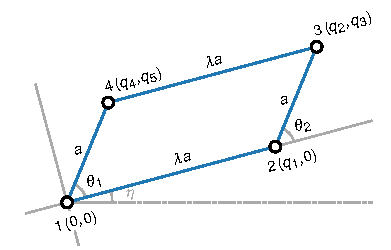
\includegraphics{frameworks/4bar.pdf}
  \end{center}
  \caption{Body frame on the planar four-bar linkage with joint~1 at the origin and bar~1--2 lying along the horizontal axis.
    The angle between the horizontal axes of the body and lab frame is $\eta$.}
  \label{fig:4bar}
\end{figure}

\subsection{Branch parameterization}

The four-bar linkage admits two modes of deformations, giving its shape space a branched appearance.
On the parallel branch the angles $\theta_{1}$ and $\theta_{2}$ are equal, whereas on the twisted branch they have a nonlinear relationship with opposite signs.
To find the exact relationship between $\theta_{1}$ and $\theta_{2}$ on the twisted branch, we first write down the constraint equation for bar~3--4 (see Fig.~\ref{fig:4bar}) of the four-bar linkage:
%
\begin{equation}
  [\lambda a + a(\cos{\theta_2} - \cos{\theta_1})]^2 + (a\sin{\theta_2} - a\sin{\theta_1})^2 = \lambda^2 a^2.
\end{equation}
%
Assuming that the aspect ratio $\lambda \ne 1$, this equation can be simplified and factorized in two different ways to get
%
\begin{subequations}
\begin{align}
  \left[\cos{\theta_2} - \cos{\theta_1}\right]\left[\cos{\theta_2} - \frac{(1 + \lambda^2)\cos{\theta_1} - 2\lambda}{1 - 2\lambda\cos{\theta_1} + \lambda^2}\right] &= 0,\\
  \left[\sin{\theta_2} - \sin{\theta_1}\right]\left[\sin{\theta_2} - \frac{(1 - \lambda^2)\sin{\theta_1}}{1 -2\lambda\cos{\theta_1} + \lambda^2}\right] &= 0.
\end{align}
\end{subequations}
%
The solutions to the above equations tell us the relationship between the input angle $\theta_1$ and the output angle $\theta_2$ on the two branches, e.g., on the parallel branch
%
\begin{equation}
  \cos\theta_2 = \cos\theta_1,\qquad
  \sin\theta_2 = \sin\theta_1\,;
  \label{eq:parallel}
\end{equation}
%
and on the twisted branch
%
\begin{equation}
  \cos\theta_2 = \frac{(1 + \lambda^2)\cos{\theta_1} - 2\lambda}{1 - 2\lambda\cos{\theta_1} + \lambda^2}, \qquad
  \sin\theta_2 = \frac{(1 - \lambda^2)\sin{\theta_1}}{1 - 2\lambda\cos{\theta_1} + \lambda^2},
  \label{eq:twisted}
\end{equation}
%
which is what we intended to find.
We can express a point $\bar{\bm{q}}$ in the shape space $\Sigma \subset \mathbb{R}^5$ of the four-bar linkage in terms of the angles $\theta_1$ and $\theta_2$ as $\bar{\bm{q}} = [\lambda a,\, a(\lambda + \cos{\theta_2}),\, a\sin{\theta_2},\, a\cos{\theta_1},\, a\sin{\theta_1}]$.
Using Eqs.~\eqref{eq:parallel} and \eqref{eq:twisted} we find two parameterizations for $\Sigma$, namely $\psi_+: \mathbb{R} \to \mathbb{R}^5$ (parallel branch) and $\psi_-: \mathbb{R} \to \mathbb{R}^5$ (twisted branch), defined by
%
\begin{subequations}
  \begin{align}
    \psi_+(\theta_1) &= \left[\lambda a, a(\lambda + \cos{\theta_1}), a\sin{\theta_1}, a\cos{\theta_1}, a\sin{\theta_1}\right],\label{eq:4bar_param_parallel}\\
    \psi_-(\theta_1) &= \left[\lambda a, a\frac{(1-\lambda^2)(\cos{\theta_1} - 1)}{1-2\lambda\cos{\theta_1}+\lambda^2}, a\frac{(1-\lambda^2)\sin{\theta_1}}{1-2\lambda\cos{\theta_1}+\lambda^2}, a\cos{\theta_1}, a\sin{\theta_1}\right].\label{eq:4bar_param_twisted}
  \end{align}
\end{subequations}
%
The above equations define two curves in $\mathbb{R}^{5}$ parameterized by the angle $\theta_{1}$.
The induced metric on these two curves can be readily computed as
%
\begin{subequations}
  \begin{align}
    (\nabla\psi_{+})\trans\nabla\psi_+ &= \Abs{\partial{\psi_{+}}/\partial{\theta_{1}}}^{2} = 2 a^2,\label{eq:4bar_ind1}\\
    (\nabla\psi_{-})\trans\nabla\psi_- &= \Abs{\partial{\psi_{-}}/\partial{\theta_{1}}}^{2} = \frac{2a^2[1-2\lambda(1-\lambda\cos{\theta_1}+\lambda^2)\cos{\theta_1} + \lambda^4]}{(1-2\lambda\cos{\theta_1}+ \lambda^2)^2}.\label{eq:4bar_ind2}
  \end{align}
\end{subequations}

% TODO: calculate free energy as a function of theta_{2}
%A similar calculation, but parameterizing the branches using the angle $\theta_{2}$ instead, gives us
%%
%\begin{subequations}
%  \begin{align}
%    (\nabla\psi_{+})\trans\nabla\psi_+ &= \Abs{\partial{\psi_{+}}/\partial{\theta_{1}}}^{2} = 2 a^2,\label{eq:4bar_q2_ind1}\\
%    (\nabla\psi_{-})\trans\nabla\psi_- &= \Abs{\partial{\psi_{-}}/\partial{\theta_{1}}}^{2} = \frac{2a^2[1-2\lambda(1-\lambda\cos{\theta_1}+\lambda^2)\cos{\theta_1} + \lambda^4]}{(1-2\lambda\cos{\theta_1}+ \lambda^2)^2}.\label{eq:4bar_q2_ind2}
%  \end{align}
%\end{subequations}

\subsection{Marginal probability densities}

\subsubsection*{Regular values}

Now that we have explicit parameterizations of the two branches of the four-bar linkage in terms of the \ac{cv} $\theta_{1}$, we can find the marginal density $\mathscr{P}(\theta_{1})$ at regular values of $\theta_{1}$, far from the singular values, i.e., for $0 \ll \abs{\theta_{1}} \ll \pi$.
Note that for each value of $\theta_{1}$, there are two ground states---one on the parallel branch and one on the twisted branch.
This means that we need to separately find the contributions of these ground states using Eq.~\eqref{eq:mpd_regular} and then add them together to obtain $\mathscr{P}(\theta_{1})$.

Starting with constraint function for bar~1--2 and going around the linkage in counterclockwise order, we find the constraint map $f: \mathbb{R}^{5} \to \mathbb{R}^{4}$ in the body frame to be
%
\begin{equation}
  f(\bm{q}) = \left[\frac{q_1^2 - \lambda^2 a^2}{2\lambda a},\, \frac{(q_2 - q_1)^2 + q_3^2 - a^2}{2a},\, \frac{(q_4 - q_2)^2 + (q_5 - q_3)^2 - \lambda^2 a^2}{2\lambda a},\, \frac{q_4^2 + q_5^2 - a^2}{2a}\right],
\end{equation}
%
and the compatibility matrix $\mathsf{C}$ to be
%
\begin{equation}
  \mathsf{C} = \nabla f = a^{-1}\begin{pmatrix}
    \lambda^{-1}q_1 & 0 & 0 & 0 & 0 \\
    (q_1-q_2) & q_2-q_1 & q_3 & 0 & 0\\
    0 & \lambda^{-1}(q_2-q_4) & \lambda^{-1}(q_3-q_5) & \lambda^{-1}(q_4-q_2) & \lambda^{-1}(q_5-q_3)\\
  0 & 0 & 0 & q_4 & q_5
  \label{eq:4bar_compatibility}
\end{pmatrix}.
\end{equation}
At regular points $\mathsf{C}$ has full rank, which implies that the dynamical matrix $\mathsf{D} = \mathsf{C}\trans\mathsf{K}\mathsf{C}$ and the matrix $\mathsf{K}\mathsf{C}\mathsf{C}\trans$ have the same nonzero eigenvalues.
This gives $\det\,\mathsf{D}^\perp = \det\,\mathsf{K}\mathsf{C}\mathsf{C}\trans = \kappa^4\det\,\mathsf{C}\mathsf{C}\trans$.
Inserting the parameterizations from Eqs.~\eqref{eq:4bar_param_parallel} and \eqref{eq:4bar_param_twisted} into the compatibility matrix we compute $\det\,\mathsf{D}^\perp$ along the two branches as
%
\begin{subequations}
\begin{align}
  \det\,\mathsf{D}^\perp_+ &= 2\kappa^4\sin^2\theta_1,\\
  \det\,\mathsf{D}^\perp_- &= \frac{2\kappa^4\sin^2{\theta_1}[1-2\lambda(1-\lambda\cos{\theta_1}+\lambda^2)\cos{\theta_1} + \lambda^4]}{(1-2\lambda\cos{\theta_1}+\lambda^2)^2}.
\end{align}
\end{subequations}
%
The asymptotic marginal density is then
%
\begin{equation}
  \begin{aligned}
    \mathscr{P}(\theta_1) &\sim I(\theta_1)\left(\frac{2\pi}{\beta}\right)^2\left[\left|\frac{\det\,(\nabla\psi_{+})\trans\nabla\psi_+}{\det\,\mathsf{D}_+^\perp}\right|^{1/2} + \left|\frac{\det\,(\nabla\psi_{-})\trans\nabla\psi_-}{\det\,\mathsf{D}_-^\perp}\right|^{1/2}\right]\\
                                           &= 2\lambda a^{2}\left(\frac{2\pi}{\beta\kappa}\right)^2|\sin{\theta_1}|^{-1},
  \end{aligned}
  \label{eq:4bar_r}
\end{equation}
where we have used $I(\theta_{1}) = \abs{q_{1}} = \lambda a$ [Eq.~\eqref{eq:4bar_jacobian}] and the expressions for the induced metrics [Eqs.~\eqref{eq:4bar_ind1} and \eqref{eq:4bar_ind2}] computed earlier.

\subsubsection*{Singular values}

The four-bar linkage has shape-space singularities at $\theta_1 = 0$ and $\theta_1 = \pm\pi$ corresponding to configurations where the bars are collinear.
Let us first look at the singularity at $\theta_1 = 0$, where the configuration vector $\bar{\bm{q}}^{*} = [\lambda a, a(\lambda + 1), 0, a, 0]$.
The compatibility and dynamical matrices at this point are
%
\begin{equation}
  \mathsf{C} =
  \begin{pmatrix}
  1  & 0 & 0 & 0  & 0 \\
  -1 & 1 & 0 & 0  & 0 \\
  0  & 1 & 0 & -1 & 0 \\
  0  & 0 & 0 & 1  & 0 \\
  \end{pmatrix}
  \quad\text{and}\quad
  \mathsf{D} = \mathsf{C}\trans\mathsf{K}\mathsf{C} = \kappa
  \begin{pmatrix}
    2  & -1 & 0 & 0  & 0 \\
    -1 & 2  & 0 & -1 & 0 \\
    0  & 0  & 0 & 0  & 0 \\
    0  & -1 & 0 & 2  & 0 \\
    0  & 0  & 0 & 0  & 0 \\
  \end{pmatrix}.
\end{equation}
%
The dynamical matrix has nonzero eigenvalues $(2+\sqrt{2})\kappa$, $2\kappa$, and $(2-\sqrt{2})\kappa$, which gives $\det\,\mathsf{D}^\perp = 4\kappa^3$.
Also, the Hessian matrices of the four constraint functions $f_i$ at the singularity~are

\begin{equation}
\begin{aligned}
  \hess f_1 &=
  (\lambda a)^{-1}\begin{pmatrix}
    1 & 0 & 0 & 0 & 0 \\
    0 & 0 & 0 & 0 & 0 \\
    0 & 0 & 0 & 0 & 0 \\
    0 & 0 & 0 & 0 & 0 \\
    0 & 0 & 0 & 0 & 0 \\
  \end{pmatrix},\qquad {}&
  \hess f_2 &= a^{-1}
  \begin{pmatrix}
    1 & -1 & 0 & 0 & 0 \\
    -1 & 1 & 0 & 0 & 0 \\
    0 & 0 & 1 & 0 & 0 \\
    0 & 0 & 0 & 0 & 0 \\
    0 & 0 & 0 & 0 & 0 \\
  \end{pmatrix},\qquad\\
  \hess f_3 &=
  (\lambda a)^{-1}\begin{pmatrix}
    0 & 0 & 0 & 0 & 0 \\
    0 & 1 & 0 & -1 & 0 \\
    0 & 0 & 1 & 0 & -1 \\
    0 & -1 & 0 & 1 & 0 \\
    0 & 0 & -1 & 0 & 1 \\
  \end{pmatrix},\qquad {}&
  \hess f_4 &= a^{-1}
  \begin{pmatrix}
      0 & 0 & 0 & 0 & 0 \\
      0 & 0 & 0 & 0 & 0 \\
      0 & 0 & 0 & 0 & 0 \\
      0 & 0 & 0 & 1 & 0 \\
      0 & 0 & 0 & 0 & 1 \\
  \end{pmatrix}.
\end{aligned}
\end{equation}

As we remarked in the main text and in Section~\ref{sec:singular}, when using Eq.~\eqref{eq:mpd_singular} to find the marginal density $\mathscr{P}(\mathscr{\theta}_{1})$, we will not make use of the parameterizations we derived earlier [Eqs.~\eqref{eq:4bar_param_parallel} and \eqref{eq:4bar_param_twisted}].
Instead, we need to first linearize the \ac{cv} map at the singularity.
Since the \ac{cv} we have chosen for the four-bar linkage is the angle $\theta_{1}$, the CV map that computes $\theta_{1}$ from the configuration vector $\bm{q}$ is $\hat{\theta}_{1}(\bm{q}) = \tan^{-1}(q_{5}/q_{4})$.\footnote{To be more rigorous, we should be using the two-argument variant of the inverse tangent, sometimes denoted as $\mathrm{atan2}(q_{5},q_{4})$ in numerical software, so that $\theta_{1}$ is in $(-\pi, \pi]$ instead of $(-\pi/2,\pi/2)$.  This is not an issue for the linearization since $\theta_{1}$ is small.}
This map has the Jacobian $\nabla\hat{\theta}_1 = \inmat{0 & 0 & 0 & 0 & a^{-1}}$ at the singularity.
Direct inspection reveals that $(\nabla\hat{\theta}_{1})\bm{v} = \bm{0}$ for all fast modes $\bm{v} \in (\ker\mathsf{C})^{\perp}$, justifying the usage of Eq.~\eqref{eq:mpd_singular} to find $\mathscr{P}(\mathscr{\theta}_{1})$ when $\theta_{1} \to 0$.
This would not have been the case if, for instance, we had chosen the coordinate $q_{4}$ of joint~4 of the four-bar linkage (see Fig.~\ref{fig:4bar}), as our \ac{cv}.
In such a case $\nabla{q_{4}} = \inmat{0 & 0 & 0 & 1 & 0}$ and the fast modes, all of which are along the collinear bars with a nonzero fourth component, do not satisfy $(\nabla q_{4})\bm{v} = \bm{0}$.
Incidentally, in this case, the tangent vectors $\bm{t}$ at the singularity are such that $(\nabla q_{4})\bm{t} = \bm{0}$, which also makes $q_{4}$ a poor choice as the \ac{cv} since it does not capture the slow modes along $\bm{t}$.
Continuing with $\theta_{1}$ as our \ac{cv}, to evaluate the integral in Eq.~\eqref{eq:mpd_singular}, we choose the vector $\bm{u} \in \ker \mathsf{C}$ to be $\bm{u} = (0, 0, q_3, 0, q_{5})$, so that the vector $\bm{w}(\bm{u})$ is
%
\begin{equation}
  \begin{aligned}
    \bm{w}(\bm{u}) &= \left(\frac{1}{2}\bm{u}\trans \hess f_1 \bm{u},\, \frac{1}{2}\bm{u}\trans\hess f_2\bm{u},\, \frac{1}{2}\bm{u}\trans\hess f_3\bm{u},\, \frac{1}{2}\bm{u}\trans\hess f_4\bm{u} \right)\\
      &= \left[0,\,q_3^2/(2a),\,(q_3-q_5)^2/(2\lambda a),\,q_5^2/(2a)\right].
  \end{aligned}
  \label{eq:4bar_w}
\end{equation}
%
There is only one self stress $\bm{\sigma}\in \ker\mathsf{C}\trans$ at the singularity, and it is $\bm{\sigma} = \left(-1/2, -1/2, 1/2, 1/2\right)$.
Using this in Eq.~\eqref{eq:mpd_singular} along with $(\nabla\hat{\theta}_{1})\bm{u} = a^{-1}q_{5}$ and the fact that $\det\,\mathsf{D}^\perp = 4\kappa^3$, we get%
\footnote{From the argument of the Dirac delta function, we see that the ``hyperplane'' $\Xi_{\xi}$ in Eq.~\eqref{eq:mpd_singular} is just the line along $q_{5} = a\theta_{1}$ in the $q_{3}$-$q_{5}$ plane.}
%
\begin{equation}
  \begin{aligned}
    \mathscr{P}(\theta_1) %&\sim \frac{\lambda a}{2}\left(\frac{2\pi}{\beta\kappa}\right)^{3/2}\int \dd{q}_3\, \dd{q}_5\, \delta\left[(\nabla\hat{\theta}_{1})\bm{u} - \theta_1\right]\exp\left[-\frac{1}{2}\beta\kappa(\bm{\sigma}\cdot\bm{w})^2\right]\\
                                           &\sim \frac{\lambda a}{2}\left(\frac{2\pi}{\beta\kappa}\right)^{3/2}\Biggl(\int_{-\infty}^{\infty} \dd{q}_3\, \dd{q}_{5}\, \delta(a^{-1}q_{5} - \theta_{1})\\
                                           &\phantom{\sim \frac{\lambda a}{2}\left(\frac{2\pi}{\beta\kappa}\right)^{3/2}}\quad\times\exp\left\{-\frac{\beta\kappa}{32\lambda^2a^2}\left[q_3 - q_5\right]^2\left[(\lambda-1)q_3 + (\lambda+1)q_5\right]^2\right\}\Biggr)\\
                                           &= \frac{\lambda a^2}{2}\left(\frac{2\pi}{\beta\kappa}\right)^{3/2}\int_{-\infty}^{\infty} \dd{q}_3\, \exp\left\{-\frac{\beta\kappa}{32\lambda^2a^2}\left[q_3 - a\theta_{1}\right]^2\left[(\lambda-1)q_3 + (\lambda+1)a\theta_{1}\right]^2\right\}.
  \end{aligned}
  \label{eq:4bar_mpd_int}
\end{equation}
%
At this point, it is useful to revisit the convergence criteria for Eq.~\eqref{eq:mpd_singular}, i.e., the requirement that the term $\sum_{\bm{\sigma}} [\bm{\sigma}\cdot \bm{w}(\bm{u})]^{2}$ in the exponential of Eq.~\eqref{eq:mpd_singular} must only have isolated zeros. In the above equation, this term is $[q_3 - a\theta_{1}]^{2}[(\lambda-1)q_3 + (\lambda+1)a\theta_{1}]^{2}/(16\lambda^{2}a^{2})$, which has isolated zeros $q_{3} = a\theta_{1}$ and $q_{3} = (1+\lambda)a\theta_{1}/(1-\lambda)$, consistent with the convergence requirement.

To evaluate the integral in Eq.~\eqref{eq:4bar_mpd_int}, we symmetrize the expression in the exponential by changing variables $q_3 \to q_3 - (\lambda-1)^{-1}a\theta_1$, which yields
%
\begin{equation}
  \begin{aligned}
    \mathscr{P}(\theta_1) &\sim \frac{\lambda a^2}{2}\left(\frac{2\pi}{\beta\kappa}\right)^{3/2}\int_{-\infty}^{\infty} \dd q_3\, \exp\left\{-\frac{\beta\kappa(\lambda-1)^2}{32\lambda^2 a^2}\left[q_3^2 - \frac{\lambda^2 a^2\theta_1^2}{(\lambda-1)^2}\right]^2\right\}\\
                                           &= \lambda a^2\frac{(2\pi)^{3/2}}{(\beta\kappa)^{7/4}}\sqrt{\frac{\lambda{a}}{\abs{\lambda-1}}}\exp\left[-\frac{\beta\kappa\lambda^2a^2\theta_1^4}{32(\lambda-1)^2}\right]\int_{0}^{\infty} \dd x\, x^{-1/2}\exp\left(-\frac{1}{2}x^2 + \frac{\sqrt{\beta\kappa}\lambda a\theta_1^2}{4\abs{\lambda-1}}x\right)\\
                                           &= \lambda a^2\frac{(2\pi)^{3/2}}{(\beta\kappa)^{7/4}}\sqrt{\frac{\pi\lambda{a}}{\abs{\lambda-1}}}\exp\left[-\frac{\beta\kappa\lambda^2a^2\theta_1^4}{64(\lambda-1)^2}\right]D_{-1/2}\left(-\frac{\sqrt{\beta\kappa}\lambda a\theta_1^2}{4\abs{\lambda-1}}\right),
  \end{aligned}
  \label{eq:4bar_0}
\end{equation}
%
where $D_{-1/2}(\cdot)$ is the parabolic cylinder function~\cite{olver2010}.

For the singularity at $\theta_{1} = \pm\pi$, we have $\bar{\bm{q}}^{*} = [\lambda a, (\lambda-1)a, 0, -a, 0]$ and we proceed with a similar calculation.
The dynamical matrix and the Hessians of the constraint functions at this point is identical to those at $\theta_{1} = 0$.
Hence, we choose the vector $\bm{u}$ as before, yielding the same $\bm{w}(\bm{u})$ as in Eq.~\eqref{eq:4bar_w}.
However, the self stress at $\theta_1 = \pm\pi$ is different and it is $\bm{\sigma} = \left(-1/2, -1/2, -1/2, 1/2\right)$.
Using these results, we can evaluate the integral in Eq.~\eqref{eq:mpd_singular} as before to get
%
\begin{equation}
  \begin{aligned}
    \mathscr{P}(\theta_1) &\sim \frac{\lambda a^2}{2}\left(\frac{2\pi}{\beta\kappa}\right)^{3/2}\int_{-\infty}^{\infty} \dd{q}_3\, \exp\left\{-\frac{\beta\kappa(\lambda+1)^2}{32\lambda^2 a^2}\left[q_3^2 - \frac{\lambda^2 a^2(\pi-\abs{\theta_1})^2}{(\lambda+1)^2}\right]^2\right\}\\
                                           &= \lambda a^2\frac{(2\pi)^{3/2}}{(\beta\kappa)^{7/4}}\sqrt{\frac{\pi\lambda{a}}{\lambda+1}}\exp\left[-\frac{\beta\kappa\lambda^2a^2(\pi-\abs{\theta_1})^4}{64(\lambda+1)^2}\right]D_{-1/2}\left[-\frac{\sqrt{\beta\kappa}\lambda a(\pi-\abs{\theta_1})^2}{4(\lambda+1)}\right].
  \end{aligned}
  \label{eq:4bar_pi}
\end{equation}

Note that the marginal densities at the singular values of $\theta_{1}$, i.e., $\mathscr{P}(0)$ and $\mathscr{P}(\pm\pi)$, scale as $(\beta\kappa)^{-7/4}$.
Since $m = 4$ and the number of self stresses $s = 1$ at the singularities, this is consistent with the general scaling $\mathscr{P}(\xi^{*}) \sim (\beta\kappa)^{-(m/2 - s/4)}$ for singular values $\xi^{*}$ of the \ac{cv} [Eq.~\eqref{eq:scaling}].

\subsection{Free energy}

Using the marginal densities we have found for various regimes of $\theta_{1}$ [Eqs.~\eqref{eq:4bar_r}, \eqref{eq:4bar_0}, and \eqref{eq:4bar_pi}] we see that the free-energy difference of the four-bar linkage $\Delta\mathscr{A}(\theta_1) = \mathscr{A}(\theta_1) - \mathscr{A}(0) = -\beta^{-1}\ln{\mathscr{P}(\theta_1)} + \beta^{-1}\ln{\mathscr{P}(0)}$ takes the form
%
\begin{equation}
  \Delta\mathscr{A}(\theta_1) \sim
\begin{dcases}
  \beta^{-1}\left\{X^2\theta_1^4 - \ln\left[\dfrac{D_{-1/2}(-2X\theta_1^2)}{D_{-1/2}(0)}\right]\right\}, & \theta_1 \to 0\\
  \beta^{-1}\ln\left[X^{1/2}D_{-1/2}(0)\abs{\sin{\theta_1}}\right], & 0 \ll \abs{\theta_1} \ll \pi\\
  \beta^{-1}\left(X^2Y^2(\pi - \abs{\theta_1})^4 - \ln\left\{Y^{1/2}\dfrac{D_{-1/2}\left[-2XY(\pi - \abs{\theta_1})^2\right]}{D_{-1/2}(0)}\right\}\right), & \abs{\theta_1} \to \pi
\end{dcases}
  \label{eq:4bar_free}
\end{equation}
%
where $X$ and $Y$ are positive dimensionless terms independent of $\theta_1$ and defined by
%
\begin{equation}
  X = \frac{\sqrt{\beta\kappa}\lambda a}{8\abs{\lambda-1}},\qquad
  Y = \left|\frac{\lambda-1}{\lambda+1}\right|.
  \label{eq:XandY}
\end{equation}
%
From Eq.~\eqref{eq:4bar_free}, we also find the free-energy difference between the singular values $\theta_{1} = 0$ and $\theta_{1} = \pm\pi$ to be
%
\begin{equation}
  \mathscr{A}(\pm\pi) - \mathscr{A}(0) \sim -\beta^{-1}\ln{Y^{1/2}} = \frac{1}{2}\beta^{-1}\ln\left|\frac{\lambda + 1}{\lambda - 1}\right|,
\end{equation}
%
which is a purely geometric quantity.
This is exactly what we expect based on how the marginal density scales at a singular value [Eq.~\eqref{eq:scaling}], which shows that the free-energy difference must be a purely geometric quantity if the singular states support the same number of self stresses $s$.
A comparison between the numerical results and asymptotic expressions in Eq.~\eqref{eq:4bar_free} shows excellent agreement for all values of $\theta_{1}$ (Fig.~\ref{fig:4bar_free}).
%
\begin{figure}
  \begin{center}
    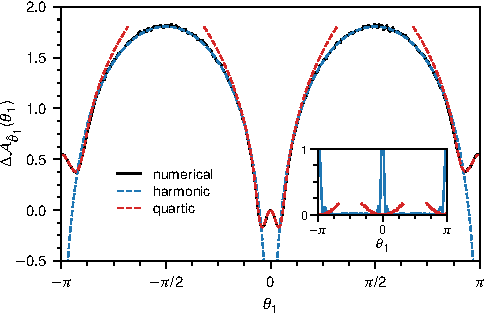
\includegraphics{frameworks/4bar_free.pdf}
  \end{center}
  \caption{Free-energy difference $\Delta\mathscr{A}(\theta_1)$ of a four-bar linkage with parameters $a=1$ and $\lambda=2$ in units of $\beta^{-1}$ at $\beta = 10^{4}$.
  The inset shows the absolute errors between the numerical and asymptotic results using the harmonic and quartic approximations [Eq.~\eqref{eq:4bar_free}].}
  \label{fig:4bar_free}
\end{figure}

Clearly, the free-energy profiles have minima for values of $\theta_{1}$ close to $0$ or $\pm\pi$, corresponding to shape-space singularities.
But a more assiduous reader may have noticed that the free-energy curves actually have a double-well minima around $\theta_{1} = 0$ and $\theta_{1} = \pm\pi$.
Also, there is an assymetry in these curves---the free energies of the four-bar linkage for $\theta_{1}$ close to $0$ is lower than $\theta_{1}$ close to $\pm\pi$.
In the next two subsections, we will try to understand these two features.

\subsubsection*{Double-well structures}

To intuitively see why the free-energy landscape of the four-bar linkage has a double-well structure centered around the singular values, consider the projection of its total energy in the space of the angles $\theta_{1}$ and $\theta_{2}$.
The projected energy can be found by setting the lengths of all bars equal to their natural lengths except for bar~3--4, which we assume to have an energy $\phi(\ell) = \kappa(\ell^{2} - \bar{\ell}^{2})^{2}/(8\bar{\ell}^{2})$.
(The exact form of the energy is irrelevant as long as it has a minimum at $\ell = \bar{\ell}$.)
Writing $\ell$ in terms of the angles $\theta_{1}, \theta_{2}$ we get
%
\begin{equation}
  \phi(\theta_{1}, \theta_{2}) = \frac{\kappa a^{2}}{8\lambda^{2}}\left[(\lambda + \cos\theta_{2} - \cos\theta_{1})^{2} + (\sin\theta_{2} - \sin\theta_{1})^{2} - \lambda^{2}\right]^{2}\,.
  \label{eq:energy34}
\end{equation}
%
Figure~\ref{fig:energy34} shows the level sets of $\phi(\theta_{1}, \theta_{2})$ near $(\theta_{1}, \theta_{2}) = (0, 0)$.
For $\abs{\theta_{1}} > 0$, there are two ground states in the \ac{cv} level set $\hat{\theta}_{1}^{-1}(\theta_{1})$, which is a straight line parallel to the $\theta_{2}$ axis in the $\theta_{1}$--$\theta_{2}$ space.
Because of the extra softness of the linkage near the singularity, this means that for small nonzero values of $\theta_{1}$, there are more thermodynamically favorable states in $\hat{\theta}_{1}^{-1}(\theta_{1})$ compared to $\hat{\theta}_{1}^{-1}(0)$, which is the \ac{cv} level set at the singular value $\theta_{1}=0$.
This is evidenced by the fact that for any given value $E > 0$, there are more points in the energy sublevel set $\left\{(\theta_{1}, \theta_{2}): \phi(\theta_{1}, \theta_{2}) \leq E\right\}$ along small nonzero values of $\theta_{1}$ than $\theta_{1} = 0$ (see Fig.~\ref{fig:energy34}).
The net increase in the number of thermodynamically favorable states near small nonzero values of $\theta_{1}$ lowers the free energy at those values, giving the landscape a double-well appearance.
%
\begin{figure}
  \begin{center}
    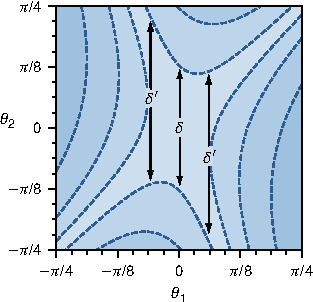
\includegraphics{frameworks/4bar_energy34.pdf}
  \end{center}
  \caption{The level sets of the energy in Eq.~\eqref{eq:energy34} around $(\theta_{1}, \theta_{2}) = (0, 0)$ for $a = \kappa = 1$ and $\lambda = 2$.  The width of the energy sublevel sets is larger along small nonzero values of $\theta_{1}$ compared to $\theta_{1} = 0$ (e.g., $\delta' > \delta$).}
  \label{fig:energy34}
\end{figure}

We also remark that since an asymptotic expression for the free energy is available for the four-bar linkage, we can explicitly show the double-well nature of $\Delta\mathscr{A}(\theta_{1})$ and find locations of its minima.
For example, expanding Eq.~\eqref{eq:4bar_0} in $\theta_{1}$ around $\theta_{1} = 0$, we see that
%
\begin{equation}
  \Delta\mathscr{A}(\theta_{1}) \sim \left[1 + 8\pi^{2}\Gamma^{-4}\left(\tfrac{1}{4}\right)\right]X^{2}\theta_{1}^{4} - 4\pi\Gamma^{-2}\left(\tfrac{1}{4}\right)X\theta_{1}^{2},\label{eq:4barwell}
\end{equation}
%
which is the equation for a double well, with $\Gamma(\cdot)$ being the gamma function.
Expanding $\Delta\mathscr{A}(\theta_{1})$ to $\mathcal{O}(\abs{\theta_{1}}^{6})$ we see that the two double-well minima are approximately at\footnote{We expand $\Delta\mathscr{A}(\theta_{1})$ to $\mathcal{O}(\abs{\theta_{1}}^{6})$ instead of $\mathcal{O}(\abs{\theta_{1}}^{4})$ since there are higher-order corrections to Eq.~\eqref{eq:4barwell} that make an $\mathcal{O}(\abs{\theta_{1}}^{4})$ estimation less accurate.}
%
\begin{equation}
  \theta_{1}^{\text{min}} \approx \pm \sqrt{\frac{\Gamma^{2}\left(\frac{1}{4}\right)\left\{8\pi^{2} + \Gamma^{4}\left(\frac{1}{4}\right) - \sqrt{\left[8\pi^{2} + \Gamma^{4}\left(\frac{1}{4}\right)\right]^{2} - (16\pi^{2})^{2}}\right\}}{64\pi^{3}X}}.
  \label{eq:thetamin}
\end{equation}
%
Since $X \sim \sqrt{\beta}$, this also shows that as $\beta$ increases, $\theta_{1}^{\text{min}}$ shifts closer to $0$.

\subsubsection*{Asymmetries in the free-energy landscape}

We will now try to understand the origin of the asymmetry in the four-bar linkage's free-energy profile, more specifically, why the free-energy values close to $\theta_{1} = \pm \pi$ is higher than the values at $\theta_{1} = 0$.
Consider Fig.~\ref{fig:4bar_asymmetry} where we show a four-bar linkage in four different configurations, but each having the same value of $\theta_{1}$.
The configurations are symmetric only along the parallel branch, where the
a configuration with $\theta_{1}$.


\begin{figure}
  \begin{center}
    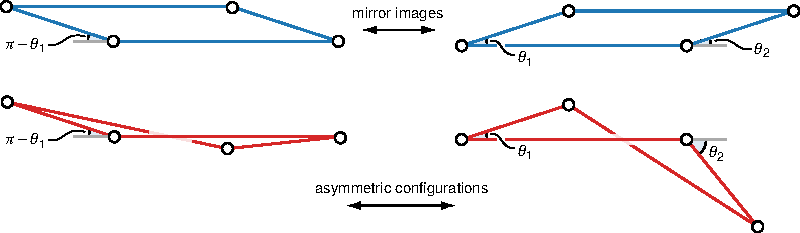
\includegraphics{frameworks/4bar_asymmetry.pdf}
  \end{center}
  \caption{%
    For values of the angle $\theta_{1} \to 0 \text{ or } \pi$, the configurations of the four-bar linkage display a certain asymmetry depending on the branch they are in.
    In case of the parallel branch, the two configurations are mirror images of each other (top figures).
    On the twisted branch, however, the two configurations are asymmetric and cannot be rotated/reflected into one another (bottom figures).
    The value of the angle $\theta_{1}$ is the same in all figures.
  }
  \label{fig:4bar_asymmetry}
\end{figure}

The asymptotic results can be obtained following the general procedure outlined in this section.

Eq.~\eqref{eq:4bar_free} after replacing the nondimensional parameters $X \to \sqrt{\beta\kappa}\lambda a/(8\abs{\lambda+1})$ and $Y \to \left|(\lambda+1)/(\lambda-1)\right|$ [cf.~Eq.~\eqref{eq:XandY}].


\section{Example: triangulated origami}
\label{sec:origami}

For further testing our methods, we consider an origami made by triangulating a unit square~\cite{chen2018} and embedded in three dimensions [Fig.~\ref{fig:origami}(a)].
To make the origami more realistic, in simulations, we avoid all configurations that result in face intersections.
The one-dimensional shape space [Fig.~\ref{fig:origami}(b)] of this origami can be visualized as four intersecting branches in the space of the fold angles, i.e., the supplement of the dihedral angle at a fold.
The intersection point is the singular flat state of the origami, where all the fold angles are zero.
After numerically parameterizing the branches of the shape space in terms of the fold angle $\rho_{1}$, which we use as our \ac{CV}, we utilize Eq.~\eqref{eq:mpd_regular} to find the free energy $\mathscr{A}(\rho_{1})$ for $\abs{\rho_{1}} \gg 0$.
We next find $\mathscr{A}(\rho_{1})$ as $\rho_{1} \to 0$ using Eq.~\eqref{eq:mpd_singular} and choose $\rho_{1}=0$ as the point of zero free energy.
A comparison between the numerical and the asymptotic results for the free-energy difference  $\Delta\mathscr{A}(\rho_{1})$ shows good agreement in both regimes of $\rho_{1}$ [Fig.~\ref{fig:origami}(c)].
Self-avoidance of the faces forces us to consider only a part of each branch of the shape space for our analysis.
Since the extent of these parts (in $\rho_{1}$) vary for the four branches [Fig.~\ref{fig:origami}(b)], it results in discontinuous jumps in the free-energy curves.
%
\begin{figure}
  \begin{center}
    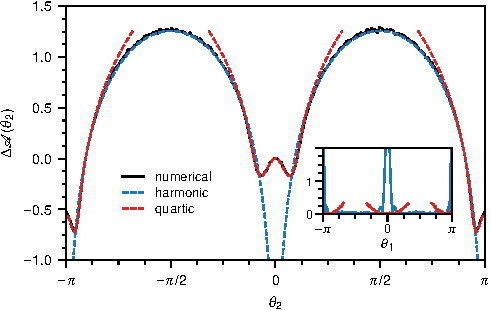
\includegraphics{frameworks/4bar_free_theta2.pdf}
  \end{center}
  \caption{Free-energy difference $\Delta\mathscr{A}(\theta_2)$ of a four-bar linkage with parameters $a=1$ and $\lambda=2$ as a function of the angle $\theta_{1}$ [cf.~Fig.~\ref{fig:4bar_free}].
  The free energy is in units of $\beta^{-1}$ at $\beta = 10^{4}$.
  Finally, the inset shows the absolute errors between the numerical and asymptotic results.
}
\end{figure}


\subsection{Body frame}

To remove the rigid motions, we transform to a body frame attached to the origami with joint~1 at the origin, bar~1--2 lying along the $x$ axis, and bar~2--6 constrained to move on the $xy$ plane [see Fig.~\ref{fig:origami}].
The origami is made out of $N = 6$ joints and $m = 11$ bars and its configuration vector $\bm{q} \in \mathbb{R}^{12}$ in the body frame is $\bm{q} = (q_{1}, q_{2}, \ldots, q_{12})$.
All orientations of the origami in the lab frame can be fully described by the two spherical polar angles that uniquely give the orientation of bar~1--2 and an azimuthal angle that gives the overall rotation of the origami about bar~1--2~\cite{herschbach1959}.
After integrating over the coordinates of joint~1 (i.e., the translational coordinates) and the three angles, and dropping constant factors, the overall Jacobian factor involved in the transformation from the lab to the body frame is $I(\bm{q}) = \abs{q_1^2 q_{12}}$.
%
\begin{figure}
  \begin{center}
    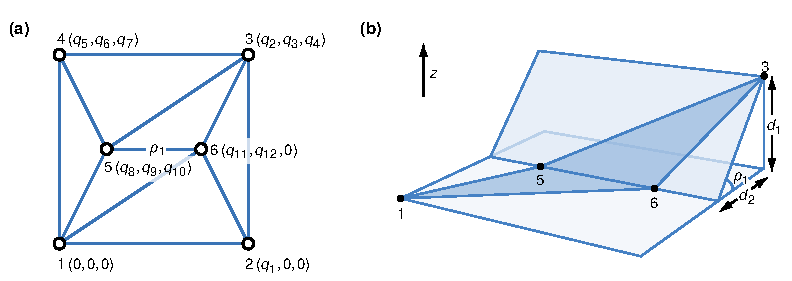
\includegraphics{frameworks/origami.pdf}
  \end{center}
  \caption{(a) A triangulated origami as a bar-joint framework illustrating the coordinates of the joints in the body frame. When the origami is flat, the external vertices lie on the corners of a unit square and the internal vertices 5 and 6 have coordinates $(1/4,1/2,0)$ and $(3/4,1/2,0)$. (b) Finding the \ac{cv} (i.e., fold angle $\rho_{1}$) using simple geometry.}
  \label{fig:origami}
\end{figure}

\subsection{Branch parameterization}

Since the shape space of the origami (and other larger frameworks) is not amenable to analytical parameterization, we have to parameterize it numerically.
We first express the tangent to the shape space at the flat state, $\bm{t}_{0} \in \ker \mathsf{C}$, in terms of its unknown components in the basis of the $(N - 3)$ out-of-plane displacement vectors of the joints.\footnote{Note that three of the $N$ joints are always constrained to move on a coordinate plane of the local Cartesian body frame.  This means that only $(N - 3)$ joints have out-of-plane displacements, and it is these displacement vectors that span $\ker\mathsf{C}$.}
An origami made by triangulating a square and having $N$ joints is expected to have at least $(N - 4)$ states of self stress $\bm{\sigma} \in \ker\mathsf{C}\trans$ when it is flat~\cite{chen2018}.
To find the components of $\bm{t}_{0}$, we then solve the $(N - 4)$ coupled quadratic equations~\cite{tarnai2001,chen2018} [see Eq.~\eqref{eq:tangentcone}]
%
\begin{equation}
  \bm{\sigma}\cdot\bm{w}(\bm{t}_{0}) = \bm{0},\quad \text{for } \bm{\sigma} \in \ker{\mathsf{C}\trans}
  \label{eq:quadratic}
\end{equation}
%
along with the normalization condition $\Abs{\bm{t}_{0}} = 1$.
Here the $i$th component of the vector $\bm{w}(\bm{t}_{0}) \in \mathbb{R}^{m}$ is $\frac{1}{2}\bm{t}_{0}\trans \hess f_{i} \bm{t}_{0}$, as in Eq.~\eqref{eq:tangentcone}. % TODO: fix eq number; this is wrong.

Numerical evidence~\cite{chen2018} suggests that one would get $2^{N-4}$ unique tangent vectors---each corresponding to a particular branch---by solving the above quadratic equations.
(Also see the related discussion regarding the solution space of these equations in Section~\ref{sec:convergence}.)
Once a tangent vector to a branch at the flat state is selected, the rest of the branch can be parameterized by numerically solving the differential equation $\dd\bm{q}/\dd{h} = \bm{t}$, where $h$ is the arc length along a branch and $\bm{t}$ is the unit tangent vector to the branch at $\bm{q}$.
If the $k$th point on the branch is $\bm{q}_k \in \mathbb{R}^{n}$, the next point $\bm{q}_{k+1}$ is then found by solving $f(\bm{q}_{k+1}) = \bm{0}$, e.g., using the Gauss--Newton method.
As the initial guess we take $\bm{q}_{k+1} = \bm{q}_{k} + \Delta h\,\bm{t}_{k}$, where $\Delta h$ is the step length along a branch.
The tangent vector $\bm{t}_k$ for $k \ne 0$ can be found by numerically computing $\ker\mathsf{C}$ at $\bm{q}_k$.
Since the tangent vectors obtained this way does not preserve direction in general, we should also multiply each $\bm{t}_k$ that is found with the sign of its dot product with the previous tangent vector $\bm{t}_{k-1}$.

On successive repetition of the above steps starting at the flat state $(\bm{q}_0, \bm{t}_0)$, we get $\bm{q}$ as a function of the arc length $h$.
To reparameterize the branch using the \ac{cv}, which is the fold angle $\rho_{1}$ of fold 5--6, we first (linearly) interpolate between the arc-length parameterized points to obtain a set of points that are uniformly spaced in $\rho_{1}$.
We then refine the interpolated points by solving $f(\bm{q}) = \bm{0}$ with the interpolated points as the initial guess.
The interpolation/refinement steps can be repeated as many times as required to achieve the desired accuracy goal.
Once the parameterization is complete, the induced metric along a branch can be computed by approximating the derivatives using difference quotients.
Note that this parameterization is only used in conjunction with Eq.~\eqref{eq:mpd_regular}.

\subsection{Marginal probability densities}

\subsubsection*{Regular values}

Similar to the calculation for the four-bar linkage, we first write down the constraint map $f: \mathbb{R}^{12} \to \mathbb{R}^{11}$ in the body frame and find the compatibility matrix $\mathsf{C} = \nabla f$.
Once all four branches of the shape space have been numerically parameterized in terms of the \ac{cv} $\rho_{1}$, the marginal probability density $\mathscr{P}(\rho_{1})$ can be computed using Eq.~\eqref{eq:mpd_regular}.
Here we remark that instead of computing $\det\,\mathsf{D}^{\perp}$ by finding the nonzero eigenvalues of $\mathsf{D}$, it is more convenient to calculate it using the fact that $\det\,\mathsf{D}^{\perp} = \det\,\mathsf{K}\mathsf{C}\mathsf{C}\trans$ at regular points.
This gives $\mathscr{P}(\rho_{1})$ for all $\rho_{1}$ far from the singular value (i.e., for $\abs{\rho_{1}} \gg 0$).

\subsubsection*{Singular value}

Our goal here is to use Eq.~\eqref{eq:mpd_singular} to find the marginal density $\mathscr{P}(\rho_{1})$ as $\rho_{1} \to 0$.
Since the calculation is similar in spirit to the case of the four-bar linkage, we only present the key steps here.
As before, we numerically compute $\det\,\mathsf{D}^{\perp}$ from the nonzero eigenvalues of $\mathsf{D}$ at the singularity.
The next step is to linearize the \ac{cv} map so that the integral in Eq.~\eqref{eq:mpd_singular} can be evaluated.

One can always numerically compute the fold angle $\rho_{1}$ as the angle between the normals to the faces that share fold 5--6.
However, for linearizing the \ac{cv} map, we need to find an expression that is more tractable analytically.
A moment's thought [and Fig.~\ref{fig:origami}(b)] shows that the \ac{cv} map can be written\footnote{To assign a sign to the fold angle, we first choose a unique normal to face 1--5--6 such that it coincides with the positive $z$ axis when the origami is flat.  Signs are then chosen so that a mountain fold (as perceived by looking downwards along this normal) has a positive fold angle, e.g., the angle in Fig.~\ref{fig:origami}(b) is negative since the fold is a valley fold.} as $\hat{\rho}_{1}(\bm{q}) = -\tan^{-1}[d_{1}(\bm{q})/d_{2}(\bm{q})]$.
Here $d_{1}(\bm{q})$ is the perpendicular distance from joint~3 to the plane containing face 1--5--6, and $d_{2}(\bm{q})$ is the perpendicular distance from the projection of joint~3 on this plane to the line along fold 5--6.
A straightforward calculation gives
%
\begin{equation}
  d_{1}(\bm{q}) = \frac{q_{10}(q_{2}q_{12} - q_{3}q_{11}) + q_4(q_{9}q_{11} - q_{8}q_{12})}{\left|q_{10}^2 q_{11}^2+q_{10}^2 q_{12}^2+(q_9 q_{11}-q_8 q_{12})^2\right|^{1/2}}.
\end{equation}
%
At the singular flat state $\bar{\bm{q}}^{*}$, we have $d_{1}(\bar{\bm{q}}^{*}) = 0$ and $d_{2}(\bar{\bm{q}}^{*}) = 0.5$, using which we find the Jacobian of the \ac{cv} map to be
%
\setcounter{MaxMatrixCols}{20}
\begin{equation}
\begin{aligned}
  \nabla\hat{\rho}_{1}(\bar{\bm{q}}^{*}) = -\frac{d_{2}(\bar{\bm{q}}^{*})\nabla d_{1}(\bar{\bm{q}}^{*}) - d_{1}(\bar{\bm{q}}^{*})\nabla d_{2}(\bar{\bm{q}}^{*})}{d^{2}_{1}(\bar{\bm{q}}^{*}) + d^{2}_{2}(\bar{\bm{q}}^{*})} &= -\frac{\nabla d_{1}(\bar{\bm{q}}^{*})}{d_{2}(\bar{\bm{q}}^{*})}\\
  &= \inmat{0 & 0 & 0 & -2 & 0 & 0 & 0 & 0 & 0 & 2 & 0 & 0}.
\end{aligned}
\end{equation}
%
Here we see that one can linearize the \ac{cv} map without needing an explicit expression for $d_{2}(\bm{q})$.
Also, it is easy to verify that $(\nabla\hat{\rho}_{1})\bm{v} = \bm{0}$ for all fast modes $\bm{v} \in (\ker\mathsf{C})^{\perp}$, enabling us to use Eq.~\eqref{eq:mpd_singular} to find the marginal density as $\rho_{1} \to 0$.

As the basis for $\ker\mathsf{C}$ we choose the out-of-plane displacements of the joints in the body frame and write the vector $\bm{u} \in \ker \mathsf{C}$ in terms of the $z$ coordinates $q_{4}$, $q_{7}$, and $q_{10}$ of the joints.
This yields $\nabla\hat{\rho}_{1}\cdot\bm{u} = 2(q_{10} - q_{4})$.
It also follows that the hyperplane $\Xi_{\xi}$ is the plane defined by $2(q_{10} - q_{4}) = \rho_{1}$ in the $q_{4}$-$q_{7}$-$q_{10}$ space and we can parameterize the points on $\Xi_{\xi}$ using either $(q_{4}, q_{7})$ or $(q_{7}, q_{10})$.
Once we write down the vector $\bm{w}(\bm{u})$ and find the self stresses $\bm{\sigma}$, we have all the ingredients to use Eq.~\eqref{eq:mpd_singular}.
However, the integral that one is left with is not amenable to analytical integration, and so we have to resort to numerical quadrature.
We do this by using a simple Monte Carlo integration scheme with $10^{9}$ sample points for each value of $\rho_{1}$ so that the maximum error is below $10^{-3}$.
One also gets near-identical results with Mathematica's numerical integrator using a global adaptive method.\footnote{\url{https:/reference.wolfram.com/language/ref/NIntegrate.html}}

\subsection{Free energy}

The free-energy difference $\Delta\mathscr{A}(\rho_{1}) = \mathscr{A}(\rho_{1}) - \mathscr{A}(0)$ for all values of $\rho_{1}$ can be easily computed from the corresponding probability densities using Eq.~\eqref{eq:free_energy}.
Similar to the four-bar linkage, the free energy of the origami also has a double-well appearance around the singular value $\rho_{1} = 0$.
This is again because of the branched nature of its shape space and the increased softness near the singularity.
%
\begin{figure*}
  \begin{center}
    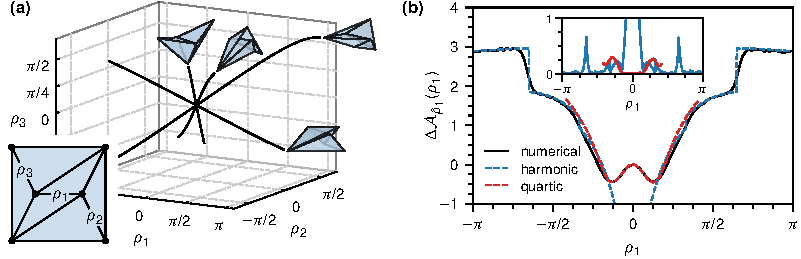
\includegraphics{frameworks/origami_free_old.pdf}
  \end{center}
  \caption{(a) A triangulated origami modeled as a bar-joint framework and (b) its shape space visualized in the space of fold angles $\rho_{1}, \rho_{2}$, and $\rho_{3}$.
    (c) Free-energy difference $\Delta\mathscr{A}(\rho_{1})$ in units of $\beta^{-1}$ at $\beta = 10^{4}$.
  The inset shows the absolute errors between the numerical and asymptotic results using the harmonic and quartic approximations (blue and red curves, respectively).}
  \label{fig:origami_free}
\end{figure*}

\section{Example: planar five-bar linkage}
\label{sec:5bar}

The example frameworks we have considered so far have one-dimensional shape spaces.
In this section, we illustrate the application of our formalism to a framework with a two-dimensional shape space, namely the planar five-bar linkage~\cite{mermoud2000,curtis2007} illustrated in Fig.~\ref{fig:5bar}(a).
The five-bar linkage we consider is made out of four bars of equal length $a$ and a fifth bar of length $2a$.
The shape space of the five-bar linkage [Fig.~\ref{fig:5bar}(b)] when visualized in the space of the angles $\zeta_{1}, \zeta_{2}$, and $\zeta_{3}$ appears as a two-dimensional surface with four isolated singularities,\footnote{At $(\zeta_{1}, \zeta_{2}, \zeta_{3}) = (0, 0, 0), (0, \pm\pi, \pm\pi), (\pm\pi, 0, \pm\pi), \text{ and } (\pm\pi, \pm\pi, 0)$.} all of which correspond to configurations where the bars become collinear and support a state of self stress.
Since force balance in self-stressed states of a planar polygonal linkage requires its bars to be collinear~\cite{farber2008}, it is not surprising that these singularities are isolated, and in their neighborhoods, the shape space is very nearly a double cone~\cite{kapovich1995,mermoud2000}.
Similar isolated singularities are also seen in the shape spaces of origami that have self-stressed flat states~\cite{berry2020}.
%
\begin{figure}
  \begin{center}
    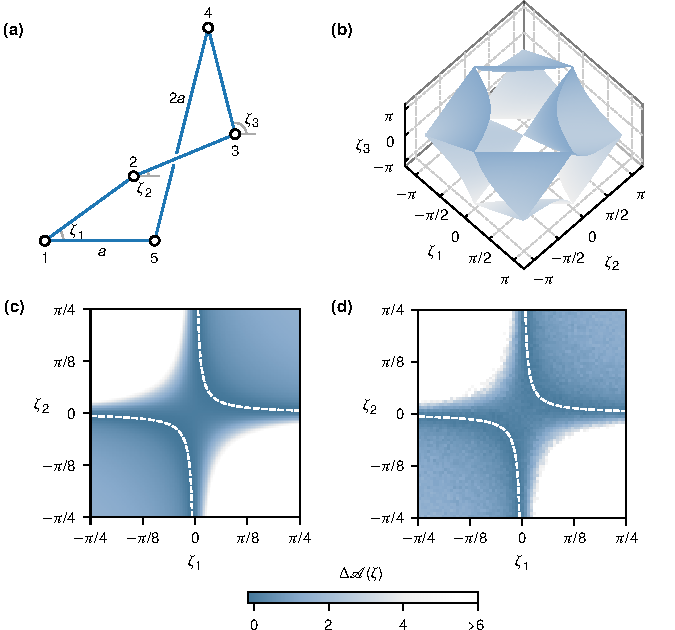
\includegraphics{frameworks/5bar.pdf}
  \end{center}
  \caption{(a) The five-bar linkage and (b) its shape space visualized in terms of the angles $\zeta_{1}, \zeta_{2},$ and $\zeta_{3}$.  These angles are measured counterclockwise from an axis parallel to bar~1--5.  Free-energy profile (in units of $\beta^{-1})$ at $\beta = 10^{4}$ around the singular value $\zeta^{*} = (0, 0)$ from (c) theory [Eq.~\eqref{eq:5bar}] and (d) simulations, with the dashed curves depicting the approximate bottom of the hyperbolic valley [Eq.~\eqref{eq:5barvalley}].}
  \label{fig:5bar}
\end{figure}


For the sake of brevity and to avoid cluttering this SM with qualitatively similar results, we only discuss the nature of the free-energy landscape around the singularity at $(\zeta_{1}, \zeta_{2}, \zeta_{3}) = (0, 0, 0)$.
Since the shape space of the five-bar linkage is two dimensional, we choose a similarly two-dimensional \ac{cv}, $\zeta = (\zeta_{1}, \zeta_{2})$.
Next, we employ Eq.~\eqref{eq:mpd_singular} to find the asymptotic free-energy difference $\Delta \mathscr{A}(\zeta)$, choosing the singular value $\zeta^{*} = (0,0)$ as the point of zero free energy.
Note that for doing this, we do not require an explicit parameterization of the linkage's shape space in terms of $\zeta$.  Such a parameterization is only required if we want to use Eq.~\eqref{eq:mpd_regular} to find the free energy far from $\zeta^{*} = (0, 0)$ using the harmonic approximation.
Since the other details are very similar to the previous calculations for the four-bar linkage and the triangulated origami, we just quote the final result:
%
\begin{equation}
  \Delta\mathscr{A}(\zeta) \sim \beta^{-1}\left\{Z^{2}\zeta_{1}^{2}\zeta_{2}^{2} - \ln\left[\frac{D_{-1/2}(-2Z\zeta_{1}\zeta_{2})}{D_{-1/2}(0)}\right]\right\},\label{eq:5bar}
\end{equation}
%
where $Z$ is a positive dimensionless term defined by $Z = \sqrt{\beta\kappa}a/(2\sqrt{5})$ [cf.~Eq.~\eqref{eq:4bar_0}].
A comparison between the theoretical and numerical results [Figs.~\ref{fig:5bar}(c) and \ref{fig:5bar}(d)] shows very good agreement between the two.
Similar to the four-bar linkage and the triangulated origami, the effective free energy minimum of the five-bar linkage is not at the singular value $\zeta^{*} = (0, 0)$.
Expanding $\Delta\mathscr{A}(\zeta)$ to $\mathcal{O}(\zeta_{1}^{3}\zeta_{2}^{3})$ around $\zeta^{*}$ we see that the bottom of the free-energy valley near the singular value [white dashed curves in Figs.~\ref{fig:5bar}(c) and \ref{fig:5bar}(d)] is approximately defined by the equation
%
\begin{equation}
  \zeta_{1}\zeta_{2} = \frac{\Gamma^{2}\left(\frac{1}{4}\right)\left\{8\pi^{2} + \Gamma^{4}\left(\frac{1}{4}\right) - \sqrt{\left[8\pi^{2} + \Gamma^{4}\left(\frac{1}{4}\right)\right]^{2} - (16\pi^{2})^{2}}\right\}}{64\pi^{3}Z},
  \label{eq:5barvalley}
\end{equation}
%
which is that of a rectangular hyperbola [cf.~Eq.~\eqref{eq:thetamin}].

\section{Permanently singular frameworks}
\label{sec:permanent}

Our discussion so far has been concerned with frameworks with isolated singularities.
In such frameworks, the constraint map $f$ drops rank only at the singularities and has full rank everywhere else.
Now consider the framework shown in Fig.~\ref{fig:trimer}(a).
The bars connecting joints~1, 2, and 3 of this framework are in a permanent state of self stress, irrespective of the value of the angle $\theta$.
By direct inspection we see that the one-dimensional shape space $\Sigma$ of this framework can be parameterized in terms of the internal angle $\theta$ using $\psi(\theta) = (a, \frac{1}{2}a, 0, a\cos{\theta}, a\sin{\theta})$.
This equation defines a smooth circle in $\mathbb{R}^{5}$, which does not have any ``visible'' singularities.
However, on inserting this parameterization into the compatibility matrix $\mathsf{C} = \nabla f$ and the dynamical matrix $\mathsf{D} = \mathsf{C}\trans\mathsf{K}\mathsf{C}$ we find (assuming that all bars have stiffness $\kappa$)
%
\begin{equation}
  \mathsf{C} =
  \begin{pmatrix}
    1 & 0 & 0 & 0 & 0 \\
    1 & -1 & 0 & 0 & 0 \\
    0 & 1 & 0 & 0 & 0 \\
    0 & 0 & 0 & \cos \theta & \sin \theta
  \end{pmatrix},
  \quad
  \mathsf{D} =
  \kappa
  \begin{pmatrix}
    2 & -1 & 0 & 0 & 0 \\
    -1 & 2 & 0 & 0 & 0 \\
    0 & 0 & 0 & 0 & 0 \\
    0 & 0 & 0 & \cos ^2\theta & \sin \theta  \cos \theta \\
    0 & 0 & 0 & \sin \theta \cos \theta & \sin ^2\theta
  \end{pmatrix}.
\end{equation}
%
Clearly, $\mathsf{C}$ is rank deficient irrespective of the value of $\theta$ and $\mathsf{D}$ has two zero modes: $\bm{t} = \dd\psi/\dd\theta \in T_{\bar{\bm{q}}}\Sigma$ corresponding to tangential motion on $\Sigma$ and a singular zero mode $\bm{u} = (0, 0, 1, 0, 0)$ associated with the self stress [see Fig.~\ref{fig:trimer}(a)].
Hence, even though the shape space here is a smooth manifold, the presence of the singular zero mode causes the harmonic approximation to break down everywhere on $\Sigma$.
This should be contrasted with the case of isolated singularities, where such singular modes appear only at the singularities of $\Sigma$.
The results that we have derived so far (namely, Eqs.~\ref{eq:mpd_regular} and \ref{eq:mpd_singular}) will not let us analyze permanently singular frameworks~\cite{muller2019,wu2020} such as the one in Fig.~\ref{fig:trimer}(a).
However, such frameworks have been considered in the context of colloidal clusters~\cite{kallus2017}.
It is thus instructive to rederive these results and compare them with our results for frameworks with isolated singularities.

Consider again a framework whose shape space $\Sigma$ is defined as the zero level set of a constraint map $f: \mathbb{R}^{n} \to \mathbb{R}^{m}$ with the compatibility matrix $\mathsf{C} = \nabla f$.
When there are $s$ permanent states of self stress, out of the $n - m + s$ zero modes that belong to $\ker\mathsf{C}$, there are $n-m$ zero modes that belong to the tangent space $T_{\bar{\bm{q}}}\Sigma$, and the remaining $s$ zero modes are the singular zero modes.
We can thus write $\ker\mathsf{C}(\bar{\bm{q}}) = T_{\bar{\bm{q}}}\Sigma \oplus \mathscr{S}$ for all $\bar{\bm{q}} \in \Sigma$.
Here $\mathscr{S}$ is the subspace of the singular zero modes at $\bar{\bm{q}}$, defined as the orthogonal complement of $T_{\bar{\bm{q}}}\Sigma$ in $\ker\mathsf{C}$.\footnote{Since the zero modes are degenerate, the singular zero modes obtained by computing $\ker\mathsf{C}$ (or $\ker\mathsf{D}$) need not be orthogonal to $T_{\bar{\bm{q}}}\Sigma$.  Hence, in writing $\ker\mathsf{C} = T_{\bar{\bm{q}}}\Sigma \oplus \mathscr{S}$, we are \emph{defining} a singular mode to be one that belongs to $\ker\mathsf{C}$, but is orthogonal to $T_{\bar{\bm{q}}}\Sigma$. Clearly, such zero modes cannot be extended to a smooth deformation of the framework.}
Note that such a decomposition of $\ker\mathsf{C}$ into two vector subspaces is not possible when $\Sigma$ has isolated singularities (where multiple branches cross) for two reasons: (i) singular zero modes exist only at the singularities of $\Sigma$ and (ii) at these singularities, there is no well-defined tangent space $T_{\bar{\bm{q}}}\Sigma$.
%
\begin{figure}
  \begin{center}
    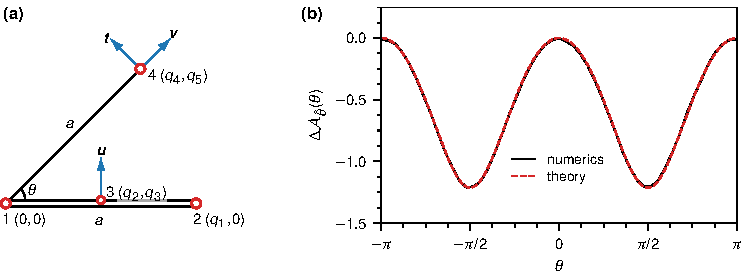
\includegraphics{frameworks/trimer.pdf}
  \end{center}
  \caption{(a) A planar framework with four joints and four bars in a body frame attached to the framework.  A bar of length $a$ connects joints~1 and~2, and two other bars of length $\frac{1}{2}a$ connect joint~3 with joints~1 and~2, which results in a state of self stress between joints 1, 2, and 3~\cite{calladine1978} for all values of $\theta$. Here $\bm{t}$ is the zero mode corresponding to tangential motion on the shape space $\Sigma$, $\bm{u}$ is a singular zero mode associated with the self stress, and $\bm{v}$ is one of the three vibrational modes.  (b) Free-energy difference $\Delta\mathscr{A}(\theta)$ [Eq.~\eqref{eq:trimer_free}] in units of $\beta^{-1}$ for a hypothetical $\theta$-dependent stiffness $\kappa(\theta) = \kappa_{0}(1 + \cos^{2}{\theta})$, chosen to verifying scaling. For constant stiffness, $\Delta\mathscr{A}(\theta)$ is zero and the free-energy landscape is flat (unlike in the case of isolated singularities).}
  \label{fig:trimer}
\end{figure}

Since the subspace $\mathscr{S}$ of singular zero modes can be identified for all points in $\Sigma$, we can expand the energy to quartic order along $\bm{u} \in \mathscr{S}$ using Eq.~\eqref{eq:energy_singular}.
(This would not have been possible for isolated singularities since Eq.~\eqref{eq:energy_singular} is valid only when the expansion is around a singularity.)
To derive the asymptotic marginal density $\mathscr{P}(\theta)$, we can then proceed similar to the derivation of Eq.~\eqref{eq:mpd_regular}.
As before, we pick coordinates associated with the framework's internal degrees of freedom as our \ac{cv} $\xi$ and assume that $\Sigma$ can be parameterized using $\xi$.
We expand both the terms in the exponent of Eq.~\eqref{eq:prob_delta} around each ground state $\bar{\bm{q}} \in \hat{\xi}^{-1}(\xi)$ after setting $\bm{q} \to \bar{\bm{q}} + \bm{t} + \bm{u} + \bm{v}$, where $\bm{t} \in T_{\bar{\bm{q}}}\Sigma$ is a zero mode that can be extended to a smooth deformation of the framework, $\bm{u} \in \mathscr{S}$ is a singular zero mode, and $\bm{v} \in (\ker\mathsf{C})^{\perp}$ is a fast mode.
We also choose the columns of $\nabla\psi(\xi)$ as the basis for $T_{\bar{\bm{q}}}\Sigma$, with $\psi: \mathbb{R}^{n-m} \to \mathbb{R}^{n}$ being the parameterization of $\Sigma$ near $\bar{\bm{q}}$.
Integrating over the components of $\bm{t}$ yields
%
\begin{equation}
  \begin{aligned}
    \mathscr{P}(\xi) &\sim I(\xi)\left(\frac{2\pi}{\beta}\right)^{(m - s)/2} \left|\det\,[\nabla\psi(\xi)]\trans\nabla\psi(\xi)\right|^{1/2} \int_{\mathscr{S}} \dd\bm{u} \int_{(\ker\mathsf{C})^{\perp}} \dd\bm{v}\, \exp\left[-\frac{1}{2}\beta\kappa\Abs{\mathsf{C}\bm{v} + \bm{w}(\bm{u})}^{2}\right]\\
                                 &= I(\xi)\left(\frac{2\pi}{\beta}\right)^{(m - s)/2}(\beta\kappa)^{-s/4} \left|\frac{\det\,[\nabla\psi(\xi)]\trans\nabla\psi(\xi)}{\det\,\mathsf{D}^{\perp}(\xi)}\right|^{1/2} \int_{\mathbb{R}^{s}} \dd\bm{x}\, \exp\left\{-\frac{1}{2}\sum_{\bm{\sigma}}[\bm{\sigma}\cdot\bm{w}(\bm{x})]^{2}\right\}.
  \end{aligned}
  \label{eq:mpd_perm}
\end{equation}
%
In the last step, we have integrated over the fast modes in $(\ker\mathsf{C})^{\perp}$ and used the results in Eqs.~\eqref{eq:mpd_gaussian}--\eqref{eq:mpd_proj}, with $\det\mathsf{D}^{\perp}$ being the product of the $m-s$ nonzero eigenvalues of the dynamical matrix $\mathsf{D}$ at $\psi(\xi)$.
Also, after picking an orthonormal basis for $\mathscr{S}$ and writing $\bm{u} = \mathsf{A}\bm{x}$, we can rescale the components $\bm{x} \to (\beta\kappa)^{-1/4}\bm{x}$ to extract all $\beta$ and $\kappa$ dependence as the term $\sum_{\bm{\sigma}} [\bm{\sigma}\cdot \bm{w}(\bm{x})]^{2}$ is a homogeneous quartic polynomial in the components of $\bm{x}$.
Equation~\eqref{eq:mpd_perm} is a rederivation of the integrand in Eq.~(14) of Ref.~\cite{kallus2017} and although it looks very similar to Eq.~\eqref{eq:mpd_singular} of the main text, it is fundamentally different.
The similarities arise due to the fact that in deriving both Eqs.~\eqref{eq:mpd_perm} and \eqref{eq:mpd_singular}, we used the same quartic-order expansion of the energy.
Nonetheless, it is worthwhile to compare the two equations.
We can identify four major differences.

\paragraph{Integration domain.}
The integration domain in Eq.~\eqref{eq:mpd_perm} is $\mathscr{S}$, the subspace of singular zero modes, which exists for all configurations of a permanently singular framework.
In comparison, when the framework has isolated singularities, singular zero modes arise only at these singularities.
Furthermore, the domain of integration in Eq.~\eqref{eq:mpd_singular} is a \ac{cv}-dependent hyperplane $\Xi_{\xi} = (\nabla\hat{\xi})^{-1}(\xi - \xi^{*}) \cap \ker\mathsf{C}$, which is not the subspace of singular zero modes, and such a vector subspace cannot be identified for a framework with isolated singularities.

\paragraph{Relation to the shape space.}
Using Eq.~\eqref{eq:mpd_perm} requires a parameterization $\psi(\xi)$ of the shape-space $\Sigma$ and the factor $\det\,(\nabla\psi)\trans\nabla\psi$ is the determinant of the induced metric on $\Sigma$.
This is similar to Eq.~\eqref{eq:mpd_regular}, which is the harmonic marginal density.
In contrast, Eq.~\eqref{eq:mpd_singular} does not make an explicit reference to $\Sigma$ and does not involve any parameterization of its branches.
Equation~\eqref{eq:mpd_singular} acquires the factor $\abs{\det\,{\nabla\hat{\xi}}(\nabla\hat{\xi})\trans}^{-1}$ from Eq.~\eqref{eq:coarea}, which a corollary of the coarea formula.
Also, Eq.~\eqref{eq:mpd_perm} is valid for all values of $\xi$, whereas Eq.~\eqref{eq:mpd_singular} is only valid when $\xi$ is close to a singular value $\xi^{*}$ of the \ac{cv}.

\paragraph{Convergence.}
If a permanently singular framework becomes second-order rigid (see Section~\ref{sec:convergence}) once the zero modes are restricted to the subspace $\mathscr{S}$, then $\bm{\sigma}\cdot\bm{w}(\bm{x}) > 0$ for all $\bm{\sigma}$ and the integral in Eq.~\eqref{eq:mpd_perm} converges~\cite{kallus2017}.
In particular, it will not converge for frameworks that are rigid, but not second-order rigid in $\mathscr{S}$ (e.g., see the example in Appendix A.3 of Ref.~\cite{connelly1996}).
This should be contrasted with the case of Eq.~\eqref{eq:mpd_singular} where there would always be vectors $\bm{t}$ in the integration domain $\Xi_{\xi}$ that satisfy $\bm{\sigma}\cdot\bm{w}(\bm{t}) = 0$ (each corresponding to a tangent to the branch at the singularity).
Hence, convergence of Eq.~\eqref{eq:mpd_singular} relies on the requirement that the number of such vectors is finite. Two necessary conditions required for this are (i) the tangents $\bm{t}$ are resolvable at second order and (ii) the \ac{cv} map is such that $(\nabla\hat{\xi})\bm{t} \neq \bm{0}$ for all $\bm{t}$ (see Section~\ref{sec:convergence}).

\paragraph{Scaling.}
The scaling of Eq.~\eqref{eq:mpd_perm} with respect to $\beta$ is consistent with Eq.~(9) of Ref.~\cite{kallus2017}.
Furthermore, since the scaling is independent of the value of the \ac{cv} $\xi$, one would generically expect the free-energy barriers in a permanently singular framework to be dominated by entropic effects and the landscape would have the same appearance for all values of $\beta$ (provided it is large).
Contrast this with Eq.~\eqref{eq:mpd_singular}, where the term in the exponent is an inhomogeneous quartic polynomial in the components of $\bm{u}$ for $\xi \neq \xi^{*}$ (see Section~\ref{sec:scaling}).
This makes the scaling nontrivial and gives rise to temperature-dependent barriers in the free-energy landscape.

Returning to the example framework in Fig.~\ref{fig:trimer}(a), using Eq.~\eqref{eq:mpd_perm}, we find the marginal density $\mathscr{P}(\theta)$ and the free-energy difference $\Delta\mathscr{A}(\theta) = -\beta^{-1}\ln\mathscr{P}(\theta) + \beta^{-1}\ln\mathscr{P}(0)$ to be
%
\begin{equation}
  \mathscr{P}(\theta) = \Gamma\left(\tfrac{1}{4}\right)\left|\frac{2\pi^{6}a^{10}}{3(\beta\kappa)^{7}}\right|^{1/4},
  \quad
  \Delta\mathscr{A}(\theta) = \frac{7}{4}\beta^{-1}\ln\left[\frac{\kappa(\theta)}{\kappa(0)}\right].
  \label{eq:trimer_free}
\end{equation}
%
Above, we have allowed for a hypothetical $\theta$-dependent stiffness $\kappa(\theta)$ so that the scaling factor $7/4$ can be verified.
The numerical results in Fig.~\ref{fig:trimer}(b) show excellent agreement with the analytical predictions.
If the stiffness $\kappa$ is a constant, then $\Delta\mathscr{A}(\theta)$ vanishes for all values of $\theta$ and the landscape becomes flat.
This should be contrasted with the examples for frameworks with isolated singularities, where temperature-dependent free-energy barriers exist even for constant stiffness.


\section{Conclusion}

In this chapter we have described a formalism to find the free-energy landscapes of common bar-joint frameworks with isolated singularities in their shape spaces.
Our results indicate that configurations in the neighborhood of the singularities have relatively lower free energy compared to configurations farther from the singularities.
More specifically, the free-energy landscapes of the four-bar linkage and the triangulated origami [Figs.~\ref{fig:4bar_free} and \ref{fig:origami}(c)] demonstrate that the measured values of the \ac{cv} tend to be closer to their values near the singularities.
Yet, as free-energy landscapes (and even their extrema) do not always have a \ac{cv}-agnostic interpretation~\cite{e2004,hartmann2007,frenkel2013}, to draw conclusions we should also consider the physical meaning of the chosen CV.
The \ac{cv}s we picked for both the example frameworks were internal angles whose values dictate the overall shape of the framework.
Specifically, according to our results, we expect the bars of the four-bar linkage to tend to be collinear, as measured by the angle $\theta_1$ being close to $0$ or $\pi$.
Similarly, the origami will tend towards being flat, as measured by the fold angle $\rho_1$.
This tendency increases at lower temperatures as the free-energy barriers become larger.
Finally, we remark on the apparent double-well nature of the landscapes near singular values of the \ac{cv}.
Because of the branched nature of the shape spaces, when $\theta_{1} \to 0,\,\pm\pi$ or when $\rho_{1} \to 0$, there are multiple ground states where the framework is also relatively soft.
This is illustrated by the widening of the sublevel sets of the energy as one moves away from the singularity (e.g., see Fig.~\ref{fig:energy34}).
The net result is an increase in the number of thermodynamically favorable states with $\theta_{1}$ close to $0$ or $\pm\pi$ (and $\rho_{1}$ close to $0$), causing an apparent lowering of the free energy.

This could help in programming the conformational dynamics of nanoframeworks~\cite{dunn2015}.
Our findings also highlight the interplay between the geometry of a framework's shape space and its thermodynamic properties.
Since changes in configuration space topology is known to drive equilibrium phase transitions in certain physical systems~\cite{kastner2008}, it would then be interesting to consider how shape-space singularities affect the physical properties of frameworks in the thermodynamic limit.
Indeed, the affinity for the origami to be in nearly-flat configurations is reminiscent of the well-known flat phase of a polymerized membrane~\cite{abraham1990,bowick1996}, which is the natural thermodynamic limit of the triangulated origami.
Additionally, it would be interesting to explore the connection between recent mean-field theories~\cite{hernandez2022} written to describe the anomalous elastic response of cellular tissues and the results presented in this work.
The onset of rigidity in these tissues can be mapped to a critical configuration in a single cell's configuration space, rather similar to the singularities we have seen so far.\footnote{Compare, for instance, Fig.~4 of Ref.~\cite{hernandez2022} and Fig.~\ref{fig:confspaces}(c) on page~\pageref{fig:confspaces}.}
Other open questions include the behavior of these frameworks in the presence of active (nonthermal) noise~\cite{woodhouse2018}, which is known to preferentially actuate zero modes, and methods to bias their dynamics towards desired states~\cite{kang2019}, e.g., by introducing \ac{cv}-dependent bias potentials~\cite{kastner2011}.

% TODO: Daniela Kraft's paper on reconfigurable colloidal assemblies.

% TODO: There has also been considerable inter~\cite{patsyk2020}est~\cite{li2023}.

% TODO: negative thermal expansion

\begin{subappendices}

\section{Numerical simulations}
\label{sec:numerics}

For all the frameworks we consider in this work, we perform our numerical simulations%
\footnote{The code we use for Monte Carlo simulations and numerical parameterization of the shape spaces is publicly available at \url{https:/github.com/manu-mannattil/thermmech}.}
in the lab frame at an inverse temperature $\beta = 10^{4}$ using a central-force potential $\phi_i[\ell_i(\bm{r})] = [\ell_i^{2}(\bm{r}) - \bar{\ell}_i^2]^2/(8\bar{\ell}_i^2)$, which has an absolute minimum at $\ell_i = \bar{\ell}_i$, for $\ell_i \geq 0$.
With this potential, the stiffness $\kappa_{i} = \phi_i''(\bar{\ell}_i) = 1$ for all bars.
Alternatively, any other potential $\phi_{i}(\ell_{i})$ that depends only on the bar lengths and having a minimum at $\ell_{i} = \bar{\ell}_{i}$ can be used.
We find the marginal probability densities of the \ac{cv} [Eq.~\eqref{eq:mpd}] using histograms obtained from sampling the Boltzmann--Gibbs distribution using the classical Metropolis Monte Carlo algorithm (with an acceptance rate of about 50\% and $\sim 10^{9}$ samples).
The free-energy profile is then found using Eq.~\eqref{eq:free_energy}.
For the triangulated origami, there is an additional need to reject all Monte Carlo moves that lead to face crossings:
%
\begin{enumerate}
  \item For faces that share an edge [e.g., faces 1--2--6 and 2--3--6 in Fig.~\ref{fig:origami}(a)], a face crossing can be detected by looking for sign changes in the fold angle of the shared fold when it is close to $\pm \pi$.
  \item For faces that do not share an edge, we use a triangle-triangle intersection test~\cite{tropp2006} to check if they intersect.
    Since there are eight such face pairs, to reduce computational costs, we only check this when the origami is sufficiently folded.
\end{enumerate}

\section{Miscellaneous results}

In this appendix, we collect some miscellaneous results pertaining to this chapter.

\label{sub:subsection name}

\subsection*{Free energy of a stiff rotor}

Consider a rotor of unit natural length in two dimensions centered around the origin with a rotationally symmetric potential energy\footnote{We could have also chosen the more conventional energy function $U(x, y) = \kappa(\sqrt{x^2 + y^2} - 1)^2$, but that makes the integrals that follow difficult to evaluate exactly.  One can still asymptotically evaluate it by Taylor expanding $U(x, y)$ around the saddle point $y = \sqrt{1 - x^2}$ to $\mathcal{O}(y^4)$.} $U(x, y) = \kappa(x^2 + y^2 - 1)^2$, with $\kappa$ being a ``spring constant'' to set the units.
This potential energy function achieves its minimum on the unit circle $x^2 + y^2 = 1$, which is our constraint level set $\Omega$.
Choosing the $x$ coordinate of the rotor as our \ac{cv}, we have the \ac{cv} map $\hat{x}: (x,y) \mapsto x$, and the \ac{pdf} of the \ac{cv} is
%
\begin{equation}
  \begin{aligned}
    \mathscr{P}_{\hat{x}}(x) &= \int_{-\infty}^{\infty} \dd{y}\, \exp\left[-\beta\kappa(x^2 + y^2 - 1)^2\right]\\
                             &= (2\beta\kappa)^{-1/4}\exp\left[-\beta\kappa(x^2 - 1)^2\right]\,\int_{0}^{\infty} \dd{t}\,t^{-1/2}\exp\left[-\tfrac{1}{2}t^2 - \sqrt{2\beta\kappa}(x^2 - 1)t\right]\\
                             &= \sqrt{\pi}(2\beta\kappa)^{-1/4}\exp\left[-\tfrac{1}{2}\beta\kappa(x^2 - 1)^2\right]D_{-1/2}\left[\sqrt{2\beta\kappa}(x^2 - 1)\right]\,,
                             \label{eq:rotor_pdf}
  \end{aligned}
\end{equation}
%
where $D_{-1/2}[\,\cdot\,]$ is the parabolic cylinder function%
\footnote{We can also write $\mathscr{P}_{\hat{x}}(x)$ in terms of the modified Bessel function of the second kind $K_{1/4}(\,\cdot\,)$ after making use of the relation $D_{-1/2}(z) = \sqrt{z/(2\pi)}K_{1/4}(z^2/4)$ \cite[Eq.~12.7.10]{olver2010}.
This is the result that computer-algebra systems often produce.} \cite[Eq.~12.5.1]{olver2010}.
Using $\mathscr{P}_{\hat{x}}(x)$ we find the free-energy difference to be
\begin{equation}
\begin{aligned}\label{eq:rotor_exact_a}
  \mathscr{A}_{\hat{x}}(x) - \mathscr{A}_{\hat{x}}(0) &= -\beta^{-1}\log{\mathscr{P}_{\hat{x}}(x)} +\beta^{-1}\log{\mathscr{P}_{\hat{x}}(0)}\\
                                                      &= \tfrac{1}{2}\kappa(x^4 - 2x^2) - \beta^{-1}\log\left\{\frac{D_{-1/2}\left[\sqrt{2\beta\kappa}(x^2-1)\right]}{D_{-1/2}\left(-\sqrt{2\beta\kappa}\right)}\right\}\,.
\end{aligned}
\end{equation}
But what if one evaluates the integral in Eq.~\eqref{eq:rotor_pdf} asymptotically for large $\beta$ using Laplace's method?
Two (standard) parameterizations in $x$ that cover the entire circle $S^1$ are
\begin{equation}
  \psi_{\pm}(x) = (x, \pm\sqrt{1 - x^2})\,,
\end{equation}
and the corresponding induced metrics are
\begin{equation}
  |\det g_{\pm}(x)| = (1-x^2)^{-1}\,.
\end{equation}
It is clear that there is a parameterization singularity at $x = \pm 1$ where $|\det g_{\pm}(x)|$ diverges.
Meanwhile, the dynamical matrix is
\begin{equation}
  \hess U(x, \pm\sqrt{1-x^2}) = 8\kappa
  \begin{pmatrix}
    x^2 & \pm x\sqrt{1-x^2}\\
    \pm x\sqrt{1-x^2} & 1-x^2
  \end{pmatrix}\,,
\end{equation}
which has only one nonzero eigenvalue, $8\kappa$.
Making use of Eq.~\eqref{eq:mpd_regular}, we get the asymptotic \ac{pdf} (which is a rescaled $\beta$ PDF for parameters $(1/2, 1/2)$.)
\begin{equation}
  \mathscr{P}_{\hat{x}}(x) = \sqrt{\frac{\pi}{\beta\kappa(1-x^2)}} + \mathcal{O}(\beta^{-3/2})\,,
\end{equation}
which leads to
\begin{equation}\label{eq:rotor_asy_a}
  \mathscr{A}_{\hat{x}}(x) - \mathscr{A}_{\hat{x}}(0) = \beta^{-1}\log\sqrt{1-x^2}\,.
\end{equation}
\begin{figure}
  \begin{center}
    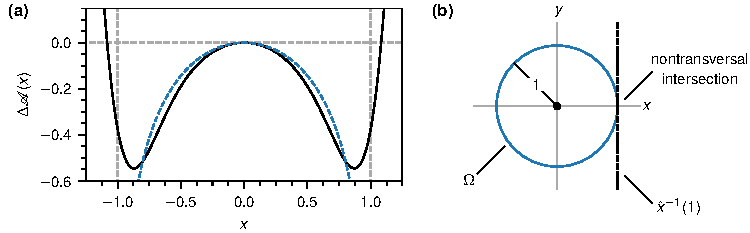
\includegraphics{fluctuations/rotor.pdf}
  \end{center}
  \caption{
    Free-energy difference $\mathscr{A}_{\hat{x}}(x) - \mathscr{A}_{\hat{x}}(0)$ of the stiff rotor at inverse temperature $\beta = 100$, from numerical simulations (black solid line), asymptotic expression (Eq.~\ref{eq:rotor_asy_a}; blue dashed line), and exact expression (Eq.~\ref{eq:rotor_exact_a}; red dashed line).
    Note how the asymptotic expression has a logarithmic divergence at $x = \pm 1$.
    Also note that the free-energy minimum is \emph{not} at $x = \pm 1$ as one might guess (or how the asymptotic expression suggests).
  }
  \label{fig:rotor}
\end{figure}

\end{subappendices}

%! TEX root = thesis.tex
% vim: ft=tex et sts=2 sw=2

\chapter{Semiclassical physics}
\label{chap04}

In this Chapter we present a quick rundown of the semiclassical approximation as applied to multicomponent waves.
To keep the exposition simple, we will restrict ourselves to wave equations in one variable.
For more detailed descriptions, we refer to the book by \citet{tracy2014}.

% This chapter is a brief discussion of elastic waves.
% In particular, we discuss waves propagating on a filament and shell, both with varying curvatures.
% The equations we derive in this chapter would form the basis of our discussions in the next chapter.

%\section{WKB analysis}

%Consider the differential equation
%%
%\begin{equation}
%  y''(x) + y(x) + \varepsilon \lambda(x) = 0.
%\end{equation}
%%
%Here $\varepsilon$ is a small parameter and suppose we wish to find solutions to this differential equation when $\varepsilon \to 0$.
%This is a \emph{regular perturbation} problem because the general characteristic features of this differential equation, namely the fact that it is second order with two independent solutions remains preserved on setting $\varepsilon = 0$.
%Hence we can attempt to find a solution of the form
%%
%\begin{equation}
%  y(x) = y_0(x) + \varepsilon y_{1}(x) + \varepsilon^{2} y_{2}(x) + \cdots
%\end{equation}
%%
%Putting this in the original differential equation, we can solve it at different orders of $\varepsilon$ to find
%%
%\begin{equation}
%  \begin{aligned}
%    \mathcal{O}(\epsilon^{0}) &: y_{0}''(x) + y_{0}(x) = 0\\
%    \mathcal{O}(\epsilon^{1}) &: y_{1}''(x) + y_{0}(x) = 0
%  \end{aligned}
%\end{equation}
%%

%The WKB method is a method to find solutions to \emph{singularly perturbed} different equations.

%Trouble might occur for instance when

%1) the highest order derivative is multiplied by $\varepsilon$.
%2) the problem totally changes characteristics when the parameter $\varepsilon$ is equal to zero.
%3) the problem is defined on infinite regions.
%4) singular points are present.
%5) the equation models physical processes with several time- or length scales.

%1-5 are called singular perturbation problems.

%In many cases we deal with problem containing boundary layers. We can roughly treat these problems by
%i) letting  we get a good approximation for the outer region.
%ii) rescale the problem to get an inner approximation.
%iii) match inner and outer approximations.

%Singular perturbation is matched asymptotic expansion.

\section{Introduction}

Consider a wave equation of the form
%
\begin{equation}
  \partial_{t}^{2}\Psi(x,t) + \widehat{\mathsf{H}}\Psi(x,t) = 0,
  \label{eq:full_wave_eq}
\end{equation}
%
where $\Psi(x,t)$ is an $N$-component wave field described by a one-dimensional coordinate $x$ and time $t$.
In elastodynamics, $\Psi$ is usually composed of displacements, e.g., for the rod we have $\Psi = (\zeta, u)$, and for the shell we have $\Psi = (\zeta, u, v)$ [see Figs.~\ref{fig:waves}(a) and~\ref{fig:waves}(b)].
Also, $\widehat{\mathsf{H}}$ is taken to be a Hermitian operator in the form of an $N\times N$ matrix, composed solely of spatial derivatives (i.e., powers of $\partial_{x}$) with time-independent coefficients.
Assuming that the waves are time harmonic with frequency $\omega$, i.e., $\Psi(x, t) = \psi(x)e^{\pm i\omega t}$, where $\psi(x)$ is the time-independent part of the wave field, Eq.~\eqref{eq:full_wave_eq} can be recast as
%
\begin{equation}
  \widehat{\mathsf{D}}\psi = 0,\quad \text{with}\enspace \widehat{\mathsf{D}} = \widehat{\mathsf{H}} - \omega^{2}\mathsf{I}_{N},
  \label{eq:ev_problem}
\end{equation}
%
where $\mathsf{I}_{N}$ is the $N\times N$ identity matrix.

If the coefficients of the spatial derivatives that appear in $\widehat{\mathsf{D}}$ are constants, then the eigenmodes $\psi$ are plain waves.
In what follows we assume that these coefficients are slowly varying, with the variation controlled by a single positive parameter $\epsilon \ll 1$, called the \emph{eikonal parameter}.
It is useful to treat $\epsilon$ as an ordering parameter so that we can look for solutions at various orders of $\epsilon$.
To this end, we rescale $x \to \epsilon^{-1}x$ so that a derivative $\partial_{x}$ becomes $\epsilon \partial x$.
With analogy to quantum mechanics, this allows us to recast the derivatives in $\widehat{\mathsf{D}}$ in terms of the wave number/momentum operator $\hat{k} = -i\epsilon \partial_{x}$, with $\epsilon$ playing the role of Planck's constant.
Since we shall be considering $\widehat{\mathsf{D}}$ in the coordinate representation, the position operator $\hat{x} = x$.

\subsection{Wave action}

An equation like Eq.~\eqref{eq:ev_problem} can be derived from a wave action of the form
%
\begin{equation}
  \begin{aligned}
    \mathscr{U}\left[\psi^{*}, \psi\right] &= \frac{1}{2}\bra{\psi}\widehat{\mathsf{D}}\ket{\psi}
  = \frac{1}{2}\int \dd{x}\,\dd{x'}\, \braket{\psi|x}\bra{x}\widehat{\mathsf{D}}\ket{x'}\braket{x'|\psi}\\
                                           &= \frac{1}{2}\int \dd{x}\dd{x'}\, \psi^{*}_{\mu}(x)\,\widehat{\mathsf{D}}_{\mu\nu}(x, x')\,\psi_{\nu}(x').
  \label{eq:wave_action}
  \end{aligned}
\end{equation}
%
Above we have inserted the resolution of identity $\int \dd{x}\,\ket{x}\bra{x} = 1$ in appropriate places to express $\mathscr{U}$ in terms of $\psi$ and its conjugate $\psi^{*}$.
Also, we have made the product between the matrix operator $\widehat{\mathsf{D}}$ and the wave vector $\psi$ explicit, with $\braket{x|\widehat{\mathsf{D}}_{\mu\nu}|x'} = \widehat{\mathsf{D}}_{\mu\nu}(x, x')$ being the matrix element of $\widehat{\mathsf{D}}_{\mu\nu}$ in the position basis.
Varying $\mathscr{U}[\psi^{*}, \psi]$ with respect to $\psi^{*}$ gives the eigenvalue problem, Eq.~\eqref{eq:ev_problem}.
For later use, we also note that $\mathscr{U}$ can also be written as
%
\begin{equation}
  \begin{aligned}
    \mathscr{U}\left[\psi^{*}, \psi\right] &= \tfrac{1}{2}\int \dd{x}' \braket{\psi_{\mu}|x'}\bra{x'}\widehat{\mathsf{D}}_{\mu\nu}\ket{\psi_{\nu}}
= \tfrac{1}{2}\int \dd{x}' \bra{x'}\widehat{\mathsf{D}}_{\mu\nu}\ket{\psi_{\nu}} \braket{\psi_{\mu}|x'}\\
&= \tfrac{1}{2}\int \dd{x}' \bra{x'}\widehat{\mathsf{D}}_{\mu\nu}\widehat{\mathsf{W}}_{\nu\mu}\ket{x'} = \tfrac{1}{2}\tr\left(\widehat{\mathsf{D}}_{\mu\nu}\widehat{\mathsf{W}}_{\nu\mu}\right),
  \label{eq:wave_action_trace_form}
  \end{aligned}
\end{equation}
%
where the matrix operator
%
\begin{equation}
  \widehat{\mathsf{W}}_{\nu\mu} = \ket{\psi_{\nu}}\bra{\psi_{\mu}},
\end{equation}
%
is the density operator.

In order to solve Eq.~\eqref{eq:ev_problem} at various orders of $\epsilon$, it is convenient to make use of Weyl calculus, which allows one to map differential operators that are functions of $\hat{x}$ and $\hat{k}$ to ordinary functions, called Weyl symbols, defined on an $x$-$k$ phase space, and vice versa~\cite{chaichian2001,cohen2012}.
For the purposes of this chapter, the following simple rules suffice to convert operators to symbols:
%
\begin{equation}
  f(x) \to f(x),\enspace
  g(\hat{k}) \to g(k),\enspace\text{and}\enspace
  f(x)g(\hat{k}) \to f(x)g(k) + \frac{i\epsilon}{2}f'(x)g'(k) + \mathcal{O}(\epsilon^{2}).
  \label{eq:weylrules}
\end{equation}
%
Above, $f$ and $g$ are functions of $x$ and $\hat{k}$, with the primes denoting derivatives.
Converting each entry of the matrix operator $\widehat{\mathsf{D}}$ into a Weyl symbol, we get the $N\times N$ dispersion matrix $\mathsf{D}$, which we express in various orders of $\epsilon$ as $\mathsf{D} = \mathsf{D}^{(0)} + \epsilon\mathsf{D}^{(1)} + \mathcal{O}(\epsilon^{2})$.

The Wigner tensor $\mathsf{W}_{\nu\mu}$ is defined as the symbol of the density operator $\widehat{\mathsf{W}} = \ket{\psi}\bra{\psi}$ with kernel $\widehat{\mathsf{W}}_{\nu\mu}(x',x) = \psi_{\nu}(x')\psi_{\mu}^{*}(x)$, and is given by
%
\begin{equation}
  \mathsf{W}_{\nu\mu}(x, k) = \int \dd{s}\, e^{-iks/\epsilon}\, \psi_{\nu}\left(x + \tfrac{1}{2}s\right)\psi^{*}_{\mu}\left(x - \tfrac{1}{2}s\right).
\end{equation}
%
By inverting the above expression, and setting $x + \frac{1}{2}s \to x'$ and $x- \frac{1}{2}s \to x$, we can write the kernel of the density operator in terms of its Weyl symbol as
%
%\begin{equation}
%  \psi_{k}\left(x + \tfrac{1}{2}s\right) \psi^{*}_{j}\left(x - \tfrac{1}{2}s\right) = \frac{1}{2\pi \epsilon} \int \dd{k}\, e^{iks/\epsilon}\,\mathsf{W}_{\nu\mu}(x, k).
%\end{equation}
%%
%so that
%
\begin{equation}
  \psi_{\nu}(x') \psi^{*}_{\mu}(x) = \frac{1}{2\pi \epsilon} \int \dd{k}\, e^{ik(x' -x)/\epsilon}\,\mathsf{W}_{\nu\mu}\left[\tfrac{1}{2}(x' + x), k\right].
  \label{eq:density_operator}
\end{equation}
%
In a similar fashion, we find
%
\begin{equation}
  \widehat{\mathsf{D}}_{\mu\nu}(x, x') = \frac{1}{2\pi\epsilon} \int \dd{l}\, e^{il(x -x')/\epsilon}\,\mathsf{D}_{\mu\nu}\left[\tfrac{1}{2}(x + x'), l\right].
  \label{eq:Dhat_integral}
\end{equation}
%
Putting Eq.~\eqref{eq:Dhat_integral} and \eqref{eq:density_operator} in Eq.~\eqref{eq:wave_action}, we arrive at
%
\begin{equation}
  \mathscr{U} = \frac{1}{2(2\pi\epsilon)^{2}}\int \dd{x}\,\dd{x'}\,\dd{k}\,\dd{l}\, e^{i(l-k)(x -x')/\epsilon}\,\mathsf{W}_{\nu\mu}\left[\tfrac{1}{2}(x' + x), k\right]\, \mathsf{D}_{\mu\nu}\left[\tfrac{1}{2}(x + x'), l\right].
\end{equation}
%
Performing the change of variables $x \to \frac{1}{2}(x + x')$ and $x' \to x - x'$, which carries a Jacobian factor of unity, we arrive at
%
\begin{equation}
  \begin{aligned}
    \mathscr{U} &= \frac{1}{2(2\pi\epsilon)^{2}}\int \dd{x}\,\dd{x'}\,\dd{k}\,\dd{l}\, e^{i(l-k)x'/\epsilon}\,\mathsf{W}_{\nu\mu}(x, k)\, \mathsf{D}_{\mu\nu}(x, l)\\
                &= \frac{1}{4\pi\epsilon}\int \dd{x}\,\dd{k}\,\mathsf{W}_{\nu\mu}(x,k)\,\mathsf{D}_{\mu\nu}(x, k).
  \end{aligned}
  \label{eq:wave_action_symbol_form}
\end{equation}

So far there has been no approximations involved and Eq.~\eqref{eq:wave_action_symbol_form} is exact to all orders of the eikonal parameter.
That said, the curious reader may wonder there is an inconsistency here, in light of Eq.~\eqref{eq:wave_action_trace_form}, where we have expressed $\mathscr{U}$ as the trace of the (scalar) operator $\widehat{O} = \widehat{\mathsf{D}}_{\mu\nu}\widehat{\mathsf{W}}_{\nu\mu}$.
In terms of its symbol, the trace of an operator $\widehat{O}$ is
%
\begin{equation}
  \tr\widehat{O} = \frac{1}{2\pi\epsilon} \int \dd{x}\,\dd{k}\, O(x, k),
\end{equation}
%
so that $\mathscr{U}$ must be
%
\begin{equation}
  \mathscr{U} = \tr{\widehat{O}} = \frac{1}{4\pi\epsilon}\int \dd{x}\,\dd{k}\, D_{\mu\nu}(x,k)e^{i\widehat{\mathcal{L}}}W_{\nu\mu}(x, k),
\end{equation}
%
where we have used the Moyal formula to write the symbol $O$ in terms of the symbols of $\mathsf{D}_{\mu\nu}$ and $\mathsf{W}_{\nu\mu}$.
The issue here is a bit subtle---the resolution is that each correction term in the Moyal series can be expressed as divergence of a vector field in the $(x, k)$ phase space~\cite[Problem 3.16]{tracy2014}.
Hence, using the divergence theorem, the integrals over the correction terms vanish for all well behaved wave fields.
Thus, only the first term in the Moyal series remains, and we get Eq.~\eqref{eq:wave_action_symbol_form} again.

Returning to our main problem, i.e., to employ the semiclassical approximation to solve Eq.~\eqref{eq:ev_problem}, we will proceed as follows: (i) insert the eikonal ansatz into the wave action; (ii) expand the action to the lowest order in the eikonal parameter and form the \emph{reduced action} $\mathscr{U}_{\text{R}}$; (iii) extract the semiclassical equations of motions by varying the reduced action.

\subsubsection*{Reduced wave action}

We look for \emph{eikonal} solutions to Eq.~\eqref{eq:ev_problem} of the form $\psi(x) = A(x)e^{iS(x)/\epsilon}$, where the amplitude $A(x)$ is an $N$-component spinor with complex components, and $S(x)$ is a rapidly varying phase, playing the role of an action.
To this end we set $\psi_{\mu} = A_{\mu}e^{iS(x)/\epsilon}$ in Eq.~\eqref{eq:wave_action_symbol_form} to obtain%
%
\begin{equation}
    \mathsf{W}_{\nu\mu}(x, k) = \int \dd{r}\,e^{ikr/\epsilon} A_{\nu}\left(x + \tfrac{1}{2} r\right)A_{\mu}^{*}\left(x - \tfrac{1}{2} r\right)\exp\left\{\frac{i}{\epsilon}\left[S\left(x + \tfrac{1}{2} r\right) - S\left(x - \tfrac{1}{2} r\right)\right]\right\}.
\end{equation}
%
Next, we set $r \to \epsilon r$ and expand the amplitude $A_{\nu}(x + \frac{1}{2}\epsilon r) = A_{\nu}(x) + \frac{1}{2}(\partial_{x}A_{\nu})\epsilon r + \mathcal{O}(\epsilon^{2})$ and the phase $S(x + \frac{1}{2}\epsilon r) = S(x) + \frac{1}{2}[\partial_{x}S(x)]\epsilon r + \mathcal{O}(\epsilon^{2})$ to obtain
%
\begin{equation}
  \begin{aligned}
    \mathsf{W}_{\nu\mu}(x, k) &= \epsilon\int \dd{r}\,e^{ikr} A_{\nu}(x)A_{\mu}^{*}(x)\exp\left\{ir\left[\partial_{x}S(x) - k\right]\right\} + \mathcal{O}(\epsilon^{2}) \\
                        &= 2\pi\epsilon A_{\nu}(x)A^{*}_{\mu}(x)\delta\left[k - \partial_{x}S(x)\right] + \mathcal{O}(\epsilon^{2}).
  \end{aligned}
\end{equation}
%
We assume that the dispersion matrix is ordered in the eikonal parameter $\epsilon$ so that we can write
$\mathsf{D} = \mathsf{D}^{(0)} + \epsilon \mathsf{D}^{(1)} + \mathcal{O}(\epsilon^{2})$.
Hence, after putting the ``reduced'' Wigner tensor in Eq.~\eqref{eq:wave_action_symbol_form}, we find the action to the lowest order as
%
\begin{equation}
  \mathscr{U} = \tfrac{1}{2}\int \dd{x}\, \mathsf{D}^{(0)}_{\mu\nu}\left[x, k=\partial_{x}S(x)\right]A_{\nu}(x)A^{*}_{\mu}(x) + \mathcal{O}(\epsilon^{2}).
  \label{eq:wave_action_reduced_1}
\end{equation}
%
Next, we perform a spectral decomposition of the lowest-order dispersion matrix $\mathsf{D}^{(0)}_{\mu\nu}(x, k)$ and write it in terms of its eigenvectors $\tau_{a}$ and eigenvalues $\lambda_{a}$ as%
\footnote{In Eq.~\eqref{eq:Dmat_polarization}, the subscripts $\mu$ and $\nu$ indicate the components of $\tau_{a}$.
Also, we have made the summation over the polarization index $a$ explicit---a convention that we will use throughout this dissertation.}
%
\begin{equation}
  \mathsf{D}^{(0)}_{\mu\nu}(x, k) = \sum_{a} \lambda_{a}(x, k) \tau_{a, \mu}(x, k) \tau_{a, \nu}^{*}(x, k).
  \label{eq:Dmat_polarization}
\end{equation}
%
As we shall see, an eigenvector $\tau_{a}$ describes a specific wave type or ``polarization'' represented by the wave equation, Eq.~\eqref{eq:ev_problem}.
And by polarization, we mean a linear subspace of the total wave field that is usually of a distinct physical nature, e.g., flexural waves on a rod.

We put Eq.~\eqref{eq:Dmat_polarization} into Eq.~\eqref{eq:wave_action_reduced_1}, and define $B_{a} = \tau_{a, \nu}^{*}A_{\nu} = \braket{\tau_{a}|A}$, which is the projection of the amplitude $A_{\nu}$ along the direction of the polarization vector $\tau_{a}$.
Although both $A_{\nu}$ and $\tau_{a}$ are general complex vectors, we can take the scalar projection $B_{a}$ to be positive by absorbing the complex phase of $A_{\nu}$ into $\tau_{a}$.
This results in a reduced action of the form
%
\begin{equation}
  \mathscr{U}_{\text{R}}\left[B_{a}, S\right] = \tfrac{1}{2} \sum_{a} \int \dd{x}\, \lambda_{a}(x,k) B_{a}^{2}(x, k),
  \quad\text{with}\quad
  k = \partial_{x}S(x).
  \label{eq:reduced_action}
\end{equation}

\subsection{Phase-space representation of waves}

Variation of the reduced action, Eq.~\eqref{eq:reduced_action}, with respect to the amplitude $B_{a}$ yields
%
\begin{equation}
  \lambda_{a}[x, k(x)]\,B_{a}[x, k(x)] = 0
  \quad\text{for all $a$}.
\end{equation}
%
Assume that the amplitudes $B_{a}$ is nonzero only for one polarization, say, $a = I$, which means that the corresponding eigenvalue must vanish:
%
\begin{equation}
  \lambda_{I}\left[x, k(x)\right] = \lambda_{I}\left[x, \partial_{x}S(x)\right] = 0.
  \label{eq:eikonal}
\end{equation}
%
The above equation, which is known as the eikonal equation, is nothing but the Hamilton--Jacobi equation with $S(x)$ playing the role of the classical action.
 This leads us to the phase-space representation of waves as rays that satisfy the Hamilton's equations
%
\begin{equation}
  \frac{\dd{x}}{\dd{\sigma}} = \partial_{k}\lambda_{I}(x, k) = \left\{x, \lambda_{I}\right\}
  \quad\text{and}\quad
  \frac{\dd{k}}{\dd{\sigma}} = -\partial_{x}\lambda_{I}(x, k) = \left\{k, \lambda_{I}\right\},
\end{equation}
%
where $\sigma$ is some parameter that parameterizes the rays $[x(\sigma), k(\sigma)]$ in the phase space, and $\left\{\cdot, \cdot\right\}$ is the $x$-$k$ Poisson bracket.
Since the waves we consider propagate in a one-dimensional space, these rays are identical to the level curve defined by $\lambda_{I}(x, k) = 0$.

In higher dimensions, solving the Hamilton-Jacobi equation can be nontrivial.
However, in one dimension, it is always theoretically possible to solve for $k(x)$ from $\lambda_{I}(x, k) = 0$.
% TODO: Tori... quantization, more stuff about Hamilton-Jacobi equations.
Variation of the action, Eq.~\eqref{eq:reduced_action}, with respect to the phase $S(x)$ yields the amplitude transport equation%
\footnote{Here we have ignored the term $\partial_{k}{B_{I}^{2}(x,k)}\lambda_{I}$, which trivially vanishes as $\lambda_{I}(x, k) = 0$ on an orbit.
Also, since $k$ is a function of $x$ on an orbit, we can simply write the projected amplitude as $B(x)$ instead of $B(x,k)$.
Note also that after evaluating the partial derivative of $\lambda_{I}$ with respect to $k$, we need to set $k \to k(x)$ for the full derivative with respect to $x$ to make sense.}
%
\begin{equation}
  \frac{\dd}{\dd{x}}\left[B^{2}_{I}(x)\partial_{k}\lambda^{(0)}_{I}(x, k)\right] = 0
\end{equation}
%
so that
$B^{2}(x,k)\partial_{k}\lambda^{(0)}_{I}(x, k) = C$ (constant) and
%
\begin{equation}
  B_{I}(x) = \frac{C}{\sqrt{\partial_{k}\lambda_{I}(x, k)}}.
\end{equation}
%
Clearly, the amplitude projection $B_{I}$ becomes singular at points on the phase space where $\dot{x} = \partial_{k}\lambda_{I}(x, k) = 0$, i.e., when the local tangent along a ray points along the $k$ axis.
Such points are called caustics, and they arise because of ill-defined projections from the ray, which lives in the $x$-$k$ phase space, to the coordinate space, i.e., $x$ space.
The issue can be sidestepped using the Keller--Maslov method~\cite{keller1958,maslov1981} where one Fourier transforms the wave field and uses the eikonal ansatz in the momentum space.
Although we shall later rely on some results of this procedure, we will not discuss its technical details here.
Interested readers are encouraged to look at the book by \citet[Chapter 6]{tracy2014} (and references therein) for more information.

In writing down the eikonal equation, Eq.~\eqref{eq:eikonal}, we have assumed that the amplitude projection $B_{a} \neq 0$ only for $a = I$.
Now, as $\mathsf{D}^{(0)}$ is a Hermitian matrix, its eigenvectors $\tau_{a}$ are mutually orthogonal, and the wave amplitude $A_{\mu} = \sum_{a} B_{a} \tau_{a,\mu} = B_{I}\tau_{I,\mu}$.
This would clearly be wrong if the matrix $\mathsf{D}^{(0)}$ is degenerate.
For this reason, usual semiclassical solutions also break down near points in the phase-space where more than one eigenvalue of $\mathsf{D}^{(0)}$ simultaneously vanish, leading to a exchange of energy and mode conversion between waves of different polarizations~\cite{tracy2014}.
As the wave problems we study in this dissertation do not suffer from mode-conversion issues (at least in the parameter ranges we are interested in), we forgo a more detailed discussion on these issues here.

Assuming that we are far away from caustics and ignoring mode-conversion effects, we can write the final eikonal solution as
%
\begin{equation}
  \psi_{\mu}(x) \sim B_{I}[x, k(x)]\,\tau_{I,\mu}[x, k(x)]e^{iS(x)/\epsilon}.
  \label{eq:psi_wkb_wrong}
\end{equation}
%
At this juncture, we must discuss a subtle problem.
The polarization vector $\tau_{I}$ is only defined up to an overall phase.
Thus, instead of the above equation, it is more appropriate to write
%
\begin{equation}
  \psi_{\mu}(x) \sim B_{I}[x, k(x)]\,\tau_{I,\mu}e^{i\gamma[x, k(x)]}e^{iS(x)/\epsilon},
\end{equation}
%
where $\gamma[x, k(x)]$ stands for an adiabatic phase that we have not determined so far.
As $\tau_{I}$ is obtained from $\mathsf{D}^{(0)}$, whose entries are slowly varying functions of $(x, k)$, it makes sense to consider the phase $\gamma[x, k(x)]$ to be slowly varying as well.
For this reason, $\gamma$ cannot be absorbed into the eikonal phase $S(x)/\epsilon$, which is rapidly varying.

The phase $\gamma$ becomes important when quantizing orbits---a step that boils down to the single valuedness of $\psi_{\mu}$ as we move around a closed orbit, i.e., the sum of $\gamma$ and $S/\epsilon$ must be a half-integral multiple of $2\pi$ (see Section~\ref{sec:bound}).
Unfortunately, our lowest-order analysis is insufficient to determine this phase.
We cannot also find an evolution equation for this phase from the reduced action, Eq.~\eqref{eq:reduced_action}, as it is independent of $\gamma$.
It can also be easily checked that the phase $\gamma$ cannot be introduced in the action by rephasing $\tau$ by the phase factor $e^{i\gamma(x,k)}$, as the action remains invariant.
The message is clear: to find $\gamma$, we need to include higher-order corrections in the wave action.
To this end, rather than repeat the original, but cumbersome derivations scattered across Refs.~\cite{bernstein1975,berk1980,yabana1986,kaufman1987}, it is more sagacious to switch gears and follow a different approach due to Littlejohn and coworkers~\cite{littlejohn1991,littlejohn1991a} for (approximately) diagonalizing multicomponent differential operators.

%Employing the eikonal ansatz, at $\mathcal{O}(\epsilon^{0})$, we find the matrix equation $\mathsf{D}^{(0)}A = 0$.
%To satisfy this equation, at least one of the $N$ eigenvalues of $\mathsf{D}^{(0)}$, say $\lambda(x, k;\, \omega)$, must vanish so that $\det \mathsf{D}^{(0)}(x, k; \omega) = 0$.
%A vanishing eigenvalue $\lambda$ and the associated normalized eigenvector $\tau$ describes different wave types or ``polarizations'' represented by Eq.~\eqref{eq:ev_problem}.
%By a polarization we mean a linear subspace of the total wave field that is usually of a distinct physical nature, e.g., flexural waves on a curved rod.
%Semiclassical approximation breaks down near points where more than one eigenvalues of $\mathsf{D}^{(0)}$ simultaneously vanish, precipitating an exchange of energy and mode conversion between waves of different polarizations~\cite{tracy2014}.

%In the absence of mode conversion, the vanishing eigenvalues of $\mathsf{D}^{(0)}$ also serve as the \emph{ray Hamiltonian} of waves of a specific polarization.
% This leads us to the phase-space representation of waves as rays that satisfy the Hamilton's equations
%%
%\begin{equation}
%  \dot{x} = \partial_{k} \lambda(x, k;\, \omega) = \left\{x, \lambda\right\}
%  \quad\text{and}\quad
%  \dot{k} = -\partial_{x} \lambda(x, k;\, \omega) = \left\{k, \lambda\right\},
%\end{equation}
%%
%where the overdot denotes derivatives with respect to a parameter that parameterizes the rays and $\left\{\cdot, \cdot\right\}$ is the $x$-$k$ Poisson bracket.
%Since the waves we consider propagate in a one-dimensional space, these rays are identical to the level curve defined by $\lambda(x, k; \omega) = 0$.
%%
% \begin{figure}
%   \begin{center}
%     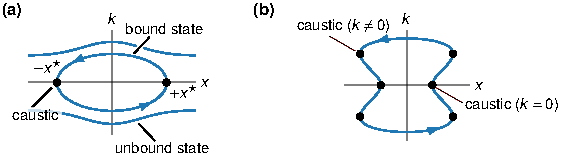
\includegraphics{localization/caustic.pdf}
%   \end{center}
%   \caption{%
%     (a) In phase space, bound states are represented by rays in the form of closed orbits, which is analogous to that of a bound particle oscillating between two classical turning points ($\pm x^{\star}$ in the cartoon).
%     Other trajectories represent unbound states.
%     (b) A bound state represented by a ``peanut''-shaped orbit has six caustics.%
%   }
%   \label{fig:caustic}
% \end{figure}

%%
%\begin{equation}
%\gamma_{\text{G}} = \oint \dd{\sigma}\, \dot{\gamma}_{\text{G}} = i\oint \dd{\sigma}\,\left\langle{\tau_{a}}\middle|\dot{\tau}_{\alpha}\right\rangle =
%  i\oint \dd\xi\cdot\left\langle{\tau_{a}}\middle|\nabla_{\xi}\tau_{\alpha}\right\rangle,
%\end{equation}
%%
%where $\xi = (x, k)$ denotes the ``parameters'' that are being varied.

%%In Appendix~\ref{app:additional_phase} we prove that $\gamma_{\text{G}}$ vanishes if the relative phases between the components of the eigenvector $\tau_{a}$ are constants.
%%The second (non-geometric) phase $\gamma_{\text{NG}}$ need not vanish in such a situation, however.
%Instead of explicitly accounting for the extra phase $\gamma$ in the quantization rule, we could have diagonalized the wave equation at various orders of $\epsilon$~\cite{littlejohn1991,littlejohn1991a,weigert1993,venaille2023}.
%During such a procedure, terms proportional to $\dot{\gamma}_{\text{G}}$ and $\dot{\gamma}_{\text{NG}}$ naturally appear in the ray Hamiltonian $\lambda$ as a first-order correction.
%Despite the elegance of the method, we do not use it in our analysis.
%This is because, as we discuss in Appendix~\ref{app:additional_phase}, for both the problems we consider, the extra phases vanish.


\section{Intermission: diagonalizing multicomponent operators}

Consider a Hermitian linear differential operator $\widehat{\mathsf{D}}$ satisfying the wave equation
%
\begin{equation}
  \widehat{\mathsf{D}}\Psi = 0,
\end{equation}
%
where $\Psi$ is an $N$-component wave field.
%
We want to find a unitary operator ${\mathsf{U}}$ such that%
\footnote{It should be emphasized that diagonalizability and unitarity are independent. For instance, let $\mathsf{U}$ be the usual unitary matrix that diagonalizes a matrix $\mathsf{D}$.
  If $\Sigma$ is some nonzero diagonal matrix, not necessarily unitary, then $(\Sigma^{\dagger}\mathsf{U}^{\dagger})\mathsf{D}(\mathsf{U}\Sigma)$ is a diagonal matrix, which follows from the fact that the product of diagonal matrices is diagonal.
  In this sense $\mathsf{U}\Sigma$ can diagonalize $\mathsf{D}$ without being unitary.}
%
\begin{equation}
  \widehat{\mathsf{U}}^{\dagger}\widehat{\mathsf{D}}\widehat{\mathsf{U}} = \widehat{\Lambda}\label{eq:diagonalization}
\end{equation}
%
is a diagonal operator.
Clearly, this equivalent to demanding that $\widehat{\mathsf{D}}\widehat{\mathsf{U}} = \widehat{\mathsf{U}}\widehat{\Lambda}$.
If we can find such an operator and solve the decoupled set of equations given by $\widehat{\Lambda}\Phi = 0$ somehow,
the solutions to the original equation can then be recovered from $\Phi$ using $\Psi = \widehat{\mathsf{U}}\Phi$.
However, Eq.~\eqref{eq:diagonalization} is an equation involving operators and standard linear algebra methods do not (directly) help in finding the unitary operator $\widehat{\mathsf{U}}$.
Instead, we start by finding the symbol form of the following two equations:
%
\begin{equation}
  \begin{aligned}
    \widehat{\mathsf{D}}\widehat{\mathsf{U}} &= \widehat{\mathsf{U}}\widehat{\Lambda}\\
    \widehat{\mathsf{U}}^{\dagger}\widehat{\mathsf{U}} &= \widehat{\mathsf{I}}_{N}.
  \end{aligned}
  \label{eq:diagonal2}
\end{equation}
%
Here we assume that the operators $\widehat{\mathsf{D}}$, $\widehat{\mathsf{U}}$, and $\widehat{\Lambda}$ have some problem-relevant ordering parameter $\epsilon$ so that we can expand%
\footnote{In their papers, Littlejohn and coworkers~\cite{littlejohn1991,weigert1993} assume that $\widehat{\mathsf{D}}$ is \emph{not} ordered in $\epsilon$, i.e., $\widehat{\mathsf{D}} = \widehat{\mathsf{D}}_{0}$.
  This might seem confusing at first since the parameter $\epsilon$ must appear somewhere in the problem.
  The thing is that very often, $\epsilon$ appears as a factor to a spatial derivative operator, e.g., $\epsilon\partial_{x}$, which once expressed in terms of the momentum operator, does not have additional dependence on $\epsilon$.
  Of course, $\widehat{\mathsf{D}}$ could have further nontrivial dependence on $\epsilon$, which is a more general situation, and the one we want to consider here.
}
the operators (and their symbols) in terms of $\epsilon$ as follows:
%
\begin{equation}
  \begin{aligned}
    \widehat{\mathsf{D}} &= \widehat{\mathsf{D}}^{(0)} + \epsilon\widehat{\mathsf{D}}^{(1)} + \epsilon^{2}\widehat{\mathsf{D}}^{(2)} + \cdots\\
    \widehat{\mathsf{U}} &= \widehat{\mathsf{U}}^{(0)} + \epsilon\widehat{\mathsf{U}}^{(1)} + \epsilon^{2}\widehat{\mathsf{U}}^{(2)} + \cdots\\
    \widehat{\Lambda} &= \widehat{\Lambda}^{(0)} + \epsilon\widehat{\Lambda}^{(1)} + \epsilon^{2}\widehat{\Lambda}^{(2)} + \cdots
  \end{aligned}
  \qquad\text{and}\qquad
  \begin{aligned}
    {\mathsf{D}} &= {\mathsf{D}}^{(0)} + \epsilon{\mathsf{D}}^{(1)} + \epsilon^{2}{\mathsf{D}}^{(2)} + \cdots\\
    {\mathsf{U}} &= {\mathsf{U}}^{(0)} + \epsilon{\mathsf{U}}^{(1)} + \epsilon^{2}{\mathsf{U}}^{(2)} + \cdots\\
    {\Lambda} &= {\Lambda}^{(0)} + \epsilon{\Lambda}^{(1)} + \epsilon^{2}{\Lambda}^{(2)} + \cdots
  \end{aligned}
\end{equation}
%
Because the Weyl correspondence preserves Hermiticity, $\mathsf{D}$ is a Hermitian matrix to all orders.
We demand that $\Lambda$ remains diagonal at all orders of $\epsilon$.
We then use the Moyal star product to find the symbol form of Eq.~\eqref{eq:diagonal2} at different orders of $\epsilon$.
At $\mathcal{O}(\epsilon^0)$ we find $\mathsf{D}^{(0)}\mathsf{U}^{(0)} = \mathsf{U}^{(0)}\Lambda^{(0)}$ and $\mathsf{U}^{(0)\dagger}\mathsf{U}^{(0)} = \mathsf{I}_{n}$, which is equivalent to
%
\begin{equation}
  \mathsf{U}^{(0)\dagger}\mathsf{D}^{(0)}\mathsf{U}^{(0)} = \Lambda^{(0)}.\label{eq:omega0}
\end{equation}
%
Since we demand $\Lambda^{(0)}$ to be diagonal, this is the usual linear-algebra problem of diagonalizing the matrix $\mathsf{D}^{(0)}$.
We thus deduce that the columns of the lowest order symbol $\mathsf{U}^{(0)}$ is composed of eigenvectors $\tau_{a}$ with eigenvalues $\lambda^{(0)}_{a}$ satisfying $\mathsf{D}^{(0)}\tau_{a} = \lambda^{(0)}_{a}\tau_{a}$, with $a = 1,2,\ldots,N$, i.e.,
%
\begin{equation}
  \mathsf{U}^{(0)} =
  \begin{pmatrix}
    \tau_{1} & \tau_{2} & \cdots & \tau_{n}
  \end{pmatrix},
\end{equation}
%
and $\Lambda^{(0)}$ is the diagonal matrix composed of the eigenvalues $\lambda_{a}^{(0)}$.

At $\mathcal{O}(\epsilon^{1})$, demanding $\mathsf{D}\mathsf{U} = \mathsf{U}\Lambda$ gives us
%
\begin{equation}
\mathsf{D}^{(1)}\mathsf{U}^{(0)} + \mathsf{D}^{(0)}\mathsf{U}^{(1)} + \frac{i}{2}\left\{\mathsf{D}^{(0)}, \mathsf{U}^{(0)}\right\} =
  \mathsf{U}^{(1)}\Lambda^{(0)} + \mathsf{U}^{(0)}\Lambda^{(1)} + \frac{i}{2}\left\{\mathsf{U}^{(0)}, \Lambda^{(0)}\right\}.
\end{equation}
%
Multiplying from the left by $\mathsf{U}^{(0)\dagger}$ and making use of $\mathsf{U}^{(0)\dagger}\mathsf{D}^{(0)} = \Lambda^{(0)}\mathsf{U}^{(0)\dagger}$, we get the $\mathcal{O}(\epsilon)$ correction%
\footnote{For further higher-order corrections to $\Lambda$, see Eq.~(19) of Ref.~\cite{weigert1993}.}
%
\begin{equation}
  \Lambda^{(1)} = \left(\mathsf{U}^{(0)\dagger}\mathsf{D}^{(1)}\mathsf{U}^{(0)} +
  \frac{i}{2}\mathsf{U}^{(0)\dagger}\left\{\mathsf{D}^{(0)},\mathsf{U}^{(0)}\right\} - \frac{i}{2}\mathsf{U}^{(0)\dagger}\left\{\mathsf{U}^{(0)},\Lambda^{(0)}\right\}\right) + \left[\Lambda^{(0)},\mathsf{U}^{(0)\dagger}\mathsf{U}^{(1)}\right].
  \label{eq:Lambda1}
\end{equation}
%
Above $[\cdot,\cdot]$ denotes the matrix commutator.
We can find $\mathsf{U}^{(0)}$ and $\Lambda^{(0)}$ by diagonalizing $\mathsf{D}^{(0)}$.
The matrix $\mathsf{D}^{(1)}$ (if it is nonzero) can be found by expanding the symbol matrix $\mathsf{D}$.
But that will still not let us find $\Lambda^{(1)}$ since we also need $\mathsf{U}^{(1)}$ to evaluate the commutator term $[\Lambda^{(0)},\mathsf{U}^{(0)\dagger}\mathsf{U}^{(1)}]$.
To proceed, we recall that we want $\Lambda$ to be diagonal at all orders, which means that $\Lambda^{(1)}$ must be a diagonal matrix as well.
The $ab$th entry of the commutator term evalutes to
%
\begin{equation}
%  \begin{aligned}
    \left[\Lambda^{(0)},\mathsf{U}^{(0)\dagger}\mathsf{U}^{(1)}\right]_{ab} = %\Lambda_{0,\alpha\gamma}\left(\mathsf{U}^{(0)\dagger}\mathsf{U}^{(1)}\right)_{\gammab} -
  %\left(\mathsf{U}^{(0)\dagger}\mathsf{U}^{(1)}\right)_{a\gamma}\Lambda_{0,\gammab}\\
    %&= \lambda_{0}^{(i)}\delta_{a\gamma}\left(\mathsf{U}^{(0)\dagger}\mathsf{U}^{(1)}\right)_{\gammab}
  %-\left(\mathsf{U}^{(0)\dagger}\mathsf{U}^{(1)}\right)_{a\gamma} \lambda_{0}^{(k)}\delta_{\gammab}\\
    \left[\lambda^{(0)}_{a} - \lambda^{(0)}_{b}\right]\left(\mathsf{U}^{(0)\dagger}\mathsf{U}^{(1)}\right)_{ab},
%  \end{aligned}
    \label{eq:diagonal}
\end{equation}
%
where we have made use of the fact that $\Lambda^{(0)}$ is diagonal so that $\Lambda^{(0)}_{ab} = \lambda^{(0)}_{a}\delta_{ab}$.
And we see that the diagonal entries (with $a=b$) of the commutator vanish.
So the commutator term does not contribute towards the diagonal entries of $\Lambda^{(1)}$ and we can find the $\mathcal{O}(\epsilon^{1})$ correction $\lambda^{(1)}$ by carefully evaluating diagonal entries of the remaining terms in the RHS of Eq.~\eqref{eq:Lambda1}.
Before we do that, we need to discuss the role of the commutator term further.
In fact, without this crucial term, the expansion will break down.

\subsection{Role of the commutator term}

None of our arguments so far guarantees that $\Lambda^{(1)}$ is diagonal.
In fact, the off-diagonal entries of four matrices in the RHS of Eq.~\eqref{eq:Lambda1} is generally not equal to zero.
The only way for $\Lambda^{(1)}$ to be diagonal then is if these off-diagonal entries somehow cancel each other.
We do not have the freedom to choose the off-diagonal entries in the first three terms since they only involve the matrices $\mathsf{U}^{(0)}$ and $\Lambda^{(0)}$, both of which are constrained by Eq.~\eqref{eq:omega0}.
However, the commutator term involves the matrix $\mathsf{U}^{(1)}$, which is something we have not found yet.
At the same time, $\mathsf{U}^{(1)}$ is not a completely arbitrary matrix, because on demanding unitarity of $\mathsf{U}$ at $\mathcal{O}(\epsilon)$ we get an additional equation that puts constraints on $\mathsf{U}^{(1)}$:
%
\begin{equation}
  \mathsf{U}^{(0)\dagger}\mathsf{U}^{(1)} + \mathsf{U}^{(1)\dagger}\mathsf{U}^{(0)} + \frac{i}{2}\left\{\mathsf{U}^{(0)\dagger}, \mathsf{U}^{(0)}\right\}= 0.
  \label{eq:unitarity}
\end{equation}
%
As we show below, this equation is not good enough to determine $\mathsf{U}^{(1)}$ completely, which is good for us since that gives us some freedom in choosing the off-diagonal elements of the commutator term in the way we want.
To simplify the commutator term we first define $\mathsf{X} = \mathsf{U}^{(0)\dagger}\mathsf{U}^{(1)}$, and from the previous equation we have
%
\begin{equation}
  \mathsf{X} + \mathsf{X}^{\dagger} = -\frac{i}{2}\left\{\mathsf{U}^{(0)\dagger}, \mathsf{U}^{(0)}\right\}.
\end{equation}
%
We see that Hermitian part of $\mathsf{X}$, given by $\mathsf{A} = (\mathsf{X} + \mathsf{X}^{\dagger})/2$, is fixed by the above equation, so that $\mathsf{A} = (-i/4)\{\mathsf{U}^{(0)\dagger},\mathsf{U}^{(0)}\}$, which is clearly a Hermitian matrix.
This still leaves us with the possibility of picking the anti-Hermitian part of $\mathsf{X}$, which we denote by $i\mathsf{B}$. Here $\mathsf{B}$ is a Hermitian matrix defined%
\footnote{%
  Writing the anti-Hermitian part of $\mathsf{X}$ this way might look nonstandard and it is more natural to write it as $(\mathsf{X} - \mathsf{X}^{\dagger})/2$.
  This is to ensure that the diagonal entries of matrix $\mathsf{B}$ are real numbers, for the sake of a future argument.
Since the matrices $\mathsf{A}$ and $\mathsf{B}$ are both Hermitian, they have real diagonals.
  These matrices each have $n^{2}$ independent entries composed of $n^{2} - n$ complex off-diagonal entries and $n$ real diagonal entries.
  All $n^{2}$ entries of $\mathsf{A}$ are fixed by $\mathsf{U}^{(0)}$.
  That leaves us with the freedom to pick the $n^{2}$ remaining entries of $\mathsf{B}$, which is good enough to ensure that $\Lambda^{(1)}$ remains diagonal.
}
by $\mathsf{B} = -i(\mathsf{X} - \mathsf{X}^{\dagger})/2$.
After replacing $\mathsf{X} = \mathsf{U}^{(0)\dagger}\mathsf{U}^{(1)}$ in the commutator term with $\mathsf{A} + i\mathsf{B}$ and using Eqs.~\eqref{eq:Lambda1} and \eqref{eq:diagonal}, we find the off-diagonal entries of $\mathsf{B}$ to be
%
\begin{equation}
  \mathsf{B}_{ab} = i\frac{\mathsf{Q}_{ab}}{\lambda^{(0)}_{a} - \lambda^{(0)}_{b}},
  \quad \text{with }a \neq b,
  \label{eq:BantiHermitian}
\end{equation}
%
where
%
\begin{equation}
  \mathsf{Q} = \mathsf{U}^{(0)\dagger}\mathsf{D}_{1}\mathsf{U}^{(0)} + \frac{i}{2}\mathsf{U}^{(0)\dagger}\left\{\mathsf{D}^{(0)},\mathsf{U}^{(0)}\right\} - \frac{i}{2}\mathsf{U}^{(0)\dagger}\left\{\mathsf{U}^{(0)},\Lambda^{(0)}\right\}
  -\frac{i}{4}\Lambda\left\{\mathsf{U}^{(0)\dagger}, \mathsf{U}^{(0)}\right\} +
  \frac{i}{4}\left\{\mathsf{U}^{(0)\dagger}, \mathsf{U}^{(0)}\right\}\Lambda.
\end{equation}
%
Although we have found an expression that gives the off-diagonal elements of $\mathsf{B}$, nothing in our arguments so far guaratees the Hermiticity of $\mathsf{B}$ and we have to explicitly check this.%
\footnote{Littlejohn and coworkers~\cite{littlejohn1991,weigert1993} seem to not have stressed this subtle point in their papers and they do not prove the Hermiticity of $\mathsf{B}$ explicitly.
  At first glance, we might think that $\mathsf{B}$ would Hermitian by construction because we \emph{took} $\mathsf{\mathsf{A}}$ and $i\mathsf{B}$ to be the Hermitian and anti-Hermitian parts of $\mathsf{X}$.
  This is not true however, as we obtained $\mathsf{A}$ from requiring unitarity of $\mathsf{U}$ at $\mathcal{O}(\epsilon)$ and we are now attempting to find the off-diagonal entries of $\mathsf{B}$ from Eq.~\eqref{eq:Lambda1}, which is an independent equation that guarantees the diagonalizability of $\mathsf{D}$ at $\mathcal{O}(\epsilon)$.
  However, there is no obvious reason why unitarity at $\mathcal{O}(\epsilon)$ should be compatible with diagonalizability at $\mathcal{O}(\epsilon)$.
  Indeed, we still need an additional requirement, i.e., the Hermiticity of $\mathsf{D}^{(1)}$ (guaranteed by the Weyl transform), for $\mathsf{B}$ to be Hermitian.
}
From Eq.~\eqref{eq:BantiHermitian}, we see that the matrix $\mathsf{Q}$ should be Hermitian if $\mathsf{B}$ is to be Hermitian.
For two general matrices $\mathsf{F}$ and $\mathsf{G}$ we have $\{\mathsf{F},\mathsf{G}\}^{\dagger} = -\{\mathsf{G}^{\dagger},\mathsf{F}^{\dagger}\}$.
Along with the assumption that $\mathsf{D}^{(1)}$ is Hermitian, we then find,
%
\begin{equation}
  \mathsf{Q}^{\dagger} =  \mathsf{U}^{(0)\dagger}\mathsf{D}^{(1)}\mathsf{U}^{(0)} + \frac{i}{2}\left\{\mathsf{U}^{(0)\dagger},   \mathsf{D}^{(0)}\right\}\mathsf{U}^{(0)} - \frac{i}{2}\left\{\Lambda^{(0)}, \mathsf{U}^{(0)\dagger}\right\}\mathsf{U}^{(0)}
  - \frac{i}{4}\left\{\mathsf{U}^{(0)\dagger}, \mathsf{U}^{(0)}\right\}\Lambda
  + \frac{i}{4}\Lambda\left\{\mathsf{U}^{(0)\dagger}, \mathsf{U}^{(0)}\right\},
\end{equation}
%
which can be further simplified%
\footnote{The simplification proceeds (by explicitly computing matrix entries) by first showing that
  $\{\mathsf{U}^{(0)\dagger}, \mathsf{D}^{(0)}\}\mathsf{U}^{(0)} = \{\mathsf{U}^{(0)\dagger}, \mathsf{U}^{(0)}\}\Lambda - \mathsf{U}^{(0)\dagger}\{\mathsf{U}^{(0)}, \Lambda\} - \{ ^{1}\mathsf{U}^{(0)\dagger}, ^{3}\mathsf{U}^{(0)}\}^{2}\mathsf{D}^{(0)}$,
  and
  $\{\Lambda^{(0)}, \mathsf{U}^{(0)\dagger}\} = \Lambda^{(0)}\{\mathsf{U}^{(0)\dagger},\mathsf{U}^{(0)}\} - \mathsf{U}^{(0)\dagger}\{\mathsf{D}^{(0)},\mathsf{U}^{(0)}\} - \{^{1}\mathsf{U}^{(0)\dagger},^{3}\mathsf{U}^{(0)}\}^{2}\mathsf{D}^{(0)}$.
  Here the superscripts 1, 2, and 3 appearing before the matrices denote the order in which they are to be multiplied; see Ref.~\cite{littlejohn1991a} for further details on this convention.
  Upon using these results in the RHS of Eq.~\fixme, we see that $\mathsf{Q}=\mathsf{Q}^{\dagger}$.
}
to show that $\mathsf{Q}^{\dagger} = \mathsf{Q}$, from which the Hermiticity of $\mathsf{B}$ follows.

Clearly, from Eq.~\eqref{eq:BantiHermitian} we see that our scheme would break down if the symbol matrix $\mathsf{D}$ has an $\mathcal{O}(\epsilon^{0})$ degeneracy, i.e., if $\mathsf{D}^{(0)}$ is degenerate with $\lambda^{(0)}_{a} = \lambda^{(0)}_{b}$ for some $a \neq b$.
For similar reasons, we cannot also determine the diagonal entries $\mathsf{B}_{aa}$ from Eq.~\eqref{eq:BantiHermitian}.
However, as we show below, we can always take them to be zero, since they do not affect the unitarity of $\mathsf{U}$ to $\mathcal{O}(\epsilon)$.
The symbol matrix $\mathsf{U}$ to $\mathcal{O}(\epsilon)$ is
%
\begin{equation}
  \mathsf{U} = \mathsf{U}^{(0)} + \epsilon \mathsf{U}^{(1)} + \mathcal{O}(\epsilon^{2}) = \mathsf{U}^{(0)}\left[\mathsf{I}_{n} + \epsilon\left(\mathsf{A} + i\mathsf{B}' + i\mathsf{B}'' \right)\right] + \mathcal{O}(\epsilon^{2}),
  \label{eq:U_with_A_and_B}
\end{equation}
%
where we have made use of $\mathsf{U}^{(1)} = \mathsf{U}^{(0)}(\mathsf{A} + i\mathsf{B})$ and have written $\mathsf{B}$ as the sum of its diagonal part $\mathsf{B}'$ and off-diagonal part $\mathsf{B}''$.%
\footnote{Since $\mathsf{B}$ is Hermitian, its diagonal part $\mathsf{B}'$ is a real matrix.}
Now, note that we have complete freedom in choosing phase factors for the columns of $\mathsf{U}^{(0)}$, namely the eigenvectors of $\mathsf{D}^{(0)}$.
Rephasing the $a$th column by $e^{-i\epsilon\mathsf{B}'_{aa}}$ turns
%
\begin{equation}
    \mathsf{U}^{(0)} \to
      \begin{pmatrix}
        e^{-i\epsilon\mathsf{B}'_{11}}\tau_{1} &
        e^{-i\epsilon\mathsf{B}'_{22}}\tau_{2} &
        \cdots &
        e^{-i\epsilon\mathsf{B}'_{nn}}\tau_{n} &
      \end{pmatrix}
      = \mathsf{U}^{(0)}(\mathsf{I}_{n} - i\epsilon\mathsf{B}') + \mathcal{O}(\epsilon^{2})
\end{equation}
%
Under the gauge transformation, the matrices $\mathsf{A} \to \mathsf{A} + \mathcal{O}(\epsilon)$ and $\mathsf{B}'' \to \mathsf{B}'' + \mathcal{O}(\epsilon)$.
Thus, the RHS of Eq.~\eqref{eq:U_with_A_and_B} becomes
%
\begin{equation}
  \left[\mathsf{U}^{(0)}(\mathsf{I}_{n} - i\epsilon\mathsf{B}') + \mathcal{O}(\epsilon^{2})\right]\left[\mathsf{I}_{n} + \epsilon\left(\mathsf{A} + i\mathsf{B}' + i\mathsf{B}'' + \mathcal{O}(\epsilon)\right)\right]
  =
  \mathsf{U}^{(0)}\left[\mathsf{I}_{n} + \epsilon\left(\mathsf{A} + i\mathsf{B}'' \right)\right] + \mathcal{O}(\epsilon^{2}).
\end{equation}
%
In other words, we can absorb any nonzero diagonal entries of $\mathsf{B}$ by a suitable rephasing of the columns of $\mathsf{U}^{(0)}$.
Thus, without loss of generality we take the diagonal part $\mathsf{B}'$ to be zero.

\subsection{First-order correction}

The matrix $\Lambda^{(1)}$, whose entries can be evaluated using the parenthetical terms in the RHS of Eq.~\eqref{eq:Lambda1}, is now fully diagonal.
The diagonal entries of $\Lambda^{(1)}$ give the first-order correction $\lambda_{a}^{(1)}$ to the eigenvalue $\lambda_{a}$ for a specific polarization, i.e., $\lambda_{a}^{(1)} = \Lambda^{(1)}_{aa}$.
We proceed by further simplifying the second and third parenthetical terms in Eq.~\eqref{eq:Lambda1} by noting that
%
\begin{equation}
  \Lambda^{(0)} = \diag\left[\lambda^{(0)}_{1}, \lambda^{(0)}_{2}, \ldots, \lambda^{(0)}_{N}\right],
  \quad
  \mathsf{U}^{(0)}_{\mu a} = \tau_{a, \mu},
  \quad\text{and}\quad
  \mathsf{U}^{(0)\dagger}_{a \mu} = \tau^{*}_{a, \mu}.
  \label{eq:Utau}
\end{equation}
%
Above, $\tau_{a, \mu}$ refers to the $\mu$th component of the polarization vector $\tau_{a}$ and $(\cdot)^{*}$ denotes complex conjugation.
Here, we have also used mixed Latin/Greek indices to separate the polarization index from the component indices (both run from $1$ to $N$, however).
Using Eq.~\eqref{eq:Utau}, the diagonal components of the first term in the parenthetical expression in Eq.~\eqref{eq:Lambda1} can be written as
%
\begin{equation}
\left(\mathsf{U}^{(0)\dagger}\mathsf{D}^{(1)}\mathsf{U}^{(0)}\right)_{aa} = \tau_{a,\mu}^{*}\mathsf{D}^{(1)}_{\mu\nu}\tau_{a,\nu}.
\label{eq:1st_term}
\end{equation}
%
Next, we simplify the diagonal entries of the second parenthetical term of Eq.~\eqref{eq:Lambda1} as
%
\begin{equation}
  \begin{aligned}
    \frac{i}{2}\left(\mathsf{U}^{(0)\dagger}  \left\{\mathsf{D}^{(0)}, \mathsf{U}^{(0)}\right\}\right)_{aa} &= \frac{i}{2}\mathsf{U}^{(0)\dagger}_{a\mu}\left(\partial_{x}\mathsf{D}^{(0)}_{\mu\nu}\partial_{k}\mathsf{U}^{(0)}_{\nu a} - \partial_{k}\mathsf{D}^{(0)}_{\mu\nu}\partial_{x}\mathsf{U}_{\nu a}^{(0)}\right)\\
                                                                                                                  &=  \frac{i}{2}\left[\partial_{x}\left(\Lambda^{(0)}_{a\mu}\mathsf{U}^{(0)\dagger}_{\mu\nu}\right) - \partial_{x}\mathsf{U}^{(0)\dagger}_{a\mu}\mathsf{D}^{(0)}_{\mu\nu}\right]\partial_{k}\mathsf{U}_{\nu a}^{(0)}\\
                                                                                                                    &\phantom{}\qquad - \frac{i}{2}\left[\partial_{k}\left(\Lambda^{(0)}_{a\mu}\mathsf{U}^{(0)\dagger}_{\mu\nu}\right) - \partial_{k}\mathsf{U}^{(0)\dagger}_{a\mu}\mathsf{D}^{(0)}_{\mu\nu}\right]\partial_{x}\mathsf{U}_{\nu a}^{(0)}\\
                                                                                                                      &= \frac{i}{2}\lambda^{(0)}_{a}\left\{\tau_{a,\mu}^{*}, \tau_{a,\mu}\right\} - \frac{i}{2}\tau_{a,\mu}^{*}\left\{\tau_{a,\mu},\lambda^{(0)}_{a}\right\} - \frac{i}{2}\mathsf{D}^{(0)}_{\mu\nu}\left\{\tau_{a,\mu}^{*}, \tau_{a,\nu}\right\}.
  \end{aligned}
  \label{eq:2nd_term}
\end{equation}
%
In the second step above, we have also made use of $\mathsf{U}^{(0)\dagger}\mathsf{D}^{(0)} = \Lambda^{(0)}\mathsf{U}^{(0)\dagger}$.
Finally, we can write the diagonal entries of the third parenthetical term in Eq.~\eqref{eq:Lambda1} as
%
\begin{equation}
  -\frac{i}{2}\left(\mathsf{U}^{(0)\dagger}\left\{\mathsf{U}^{(0)}, \Lambda^{(0)}\right\}\right)_{aa} = -\frac{i}{2}\tau_{a,\mu}^{*}\left\{\tau_{a,\mu},\lambda_{a}^{(0)}\right\}.
  \label{eq:3rd_term}
\end{equation}
%
Putting the simplified expressions from Eqs.~\eqref{eq:1st_term}--\eqref{eq:3rd_term} in Eq.~\eqref{eq:Lambda1}, we find the first-order correction in the eigenvalue $\lambda$ to be%
\footnote{This equation is identical to Eq.~(3.21) of Ref.~\cite{littlejohn1991a}, except for the first term involving $\mathsf{D}^{(1)}$, as these authors assume that the operator $\widehat{\mathsf{D}}$ is not ordered in $\epsilon$.}
%
\begin{equation}
  \boxed{
  \lambda^{(1)}_{a} = \tau_{a,\mu}^{*}\mathsf{D}_{\mu\nu}^{(1)}\tau_{a,\nu} - i\tau_{a,\mu}^{*}\left\{\tau_{a,\mu}, \lambda^{(0)}_{a}\right\} - \frac{i}{2}\left(\mathsf{D}^{(0)}_{\mu\nu} - \lambda^{(0)}_{a}\delta_{\mu\nu}\right)\left\{\tau_{a,\mu}^{*}, \tau_{a,\nu}\right\}}
  \label{eq:lambda1}
\end{equation}
%
Note that in the above equation there is no sum over the polarization index $a$, whereas the repeated Greek indices $\mu$ and $\nu$ indicate summation.

\section{Evolution of the polarization phase}

To make the transition between the variational theory presented in Section~XXX and the results in the previous section easier, we first note that
%
\begin{equation}
  \widehat{\mathsf{D}} = \widehat{\mathsf{U}}\widehat{\Lambda}\widehat{\mathsf{U}}^{\dagger}.
\end{equation}
%
Putting this in Eq.~\eqref{eq:wave_action_trace_form}, the wave action can be written as
%
\begin{equation}
  \mathscr{U} = \tfrac{1}{2}\tr\left(\widehat{\mathsf{D}}\widehat{\mathsf{W}}\right) = \tfrac{1}{2}\tr\left(\widehat{\mathsf{U}}\widehat{\Lambda}\widehat{\mathsf{U}}^{\dagger}\ket{\psi}\bra{\psi}\right) = \tfrac{1}{2}\tr\left(\widehat{\Lambda}\widehat{\mathsf{U}}^{\dagger}\ket{\psi}\bra{\psi}\widehat{\mathsf{U}}\right)
  = \tfrac{1}{2}\sum_{a} \hat{\lambda}_{a}\ket{\widetilde{\psi}_{a}}\bra{\widetilde{\psi}_{a}}
\end{equation}
%
where we have used standard results pertaining to the trace of matrix products and have defined $\ket{\widetilde{\psi}_{a}} = \widehat{\mathsf{U}}_{a\mu}\ket{\psi_{\mu}}$.
Proceeding by similar arguments as in Section~XXX, we express the wave action in terms of the Weyl symbol of the operator $\hat{\lambda}_{a}$, given by $\lambda_{a}$,  and the Wigner tensor $W_{a}$ corresponding to the density matrix $\ket{\psi}_{a}\bra{\psi}_{a}$ to find
%
\begin{equation}
  \mathscr{U} = \frac{1}{4\pi\epsilon}\sum_{a}\int \dd{x}\,\dd{k}\, \lambda_{a} W_{a}.
\end{equation}
%
The Wigner tensor $W_{a}$ to the lowest is
%
\begin{equation}
  W_{a} = \mathsf{U}^{(0)\dagger}_{a\mu}\mathsf{W}_{\mu\nu}\mathsf{U}^{(0)}_{\nu a} + \mathcal{O}(\epsilon),
\end{equation}
%
where $\mathcal{O}(\epsilon)$ represent the terms arising during the application of the Moyal formula as well as terms involving $\mathsf{U}^{(1)}$ and higher-order corrections.
One might think that it is important to find these terms, which is of the same order as the phase correction term we are after.
However, as we shall see, these terms drop out once we work out the equations of motion, and for this reason, we leave them unevaluated.
Next, we insert the eikonal ansatz for the wave fields, $\psi_{\mu} = A_{\mu}e^{iS(x)/\epsilon}$, and using the steps we followed in p.~XXX, find the reduced Wigner tensor to be
%
\begin{equation}
  \begin{aligned}
    W_{a,\text{R}} &= 2\pi \epsilon\big[\tau_{a,\nu}^{*} A_{\nu}(x)\big]\big[A^{*}_{\mu}(x)\tau_{a,\mu}\big]\delta\big[k - \partial_{x}S(x)\big] + \mathcal{O}(\epsilon^{2})\\
                   &= 2\pi\epsilon {B^{2}_{a}}(x, k)\delta\big[k - \partial_{x}S(x)\big] + \mathcal{O}(\epsilon^{2}).
  \end{aligned}
\end{equation}
%
The $\mathcal{O}(\epsilon^{2})$ above correction term now includes corrections in Eq.~XXX from the Moyal formula as well as the lowest-order expansion of the eikonal phase $S(x)$.
To $\mathcal{O}(\epsilon^{2})$, we have $\lambda_{a} = \lambda_{a}^{(0)} + \epsilon\lambda_{a}^{(1)} + \mathcal{O}(\epsilon)$, so that using Eq.~\eqref{eq:lambda1},
%
\begin{equation}
  \begin{aligned}
    \mathscr{U}\big[B_{a}, S\big] &= \mathscr{U}^{(0)}\left[B_{a}, S\right] + \epsilon\mathscr{U}^{(1)}\left[B_{a}, S\right] + \mathcal{O}(\epsilon^{2})\\
                                  &= \tfrac{1}{2} \sum_{a} \int \dd{x}\, \lambda_{a}^{(0)}(x)B^{2}_{a}(x) + \tfrac{1}{2}\epsilon\sum_{a}\int\dd{x}\,\lambda_{a}^{(1)}(x)B^{2}_{a}(x) + \mathcal{O}(\epsilon^{2}).
  \end{aligned}
\end{equation}
%
To the lowest order, the action above is equivalent to the reduced action we saw previously.
Varying the lowest-order action with respect to $B_{a}$ and $S(x)$, we find, as before, the eikonal and amplitude transport equations
%
\begin{equation}
  \begin{gathered}
    \lambda_{I}^{(0)}\big[x, k=\partial_{x}S(x)\big] = 0,\\
\frac{\dd}{\dd{x}}\left(\partial_{k}\left\{\lambda_{I}^{(0)}\big[x, k=\partial_{x}S(x)\big]B^{2}_{I}\big[x, k=\partial_{x}S(x)\big]\right\}\right) = 0.
  \end{gathered}
\end{equation}
%

Using the higher-order terms in Eq.~XXX and varying with respect to $B_{a}$, we find
%
\begin{equation}
  \lambda_{I}^{(1)}\left[x, k=\partial_{x}S(x)\right] = 0.
\end{equation}
%
Using Eq.~XXX in the above equation and noting that $\lambda_{I}^{(0)} = 0$, we find
%
\begin{equation}
\tau_{I,\mu}^{*}\mathsf{D}_{\mu\nu}^{(1)}\tau_{I,\nu} - \frac{i}{2}\mathsf{D}^{(0)}_{\mu\nu}\left\{\tau_{I,\mu}^{*}, \tau_{I,\nu}\right\}
  - i\tau_{I,\mu}\left\{\tau_{I,\mu}, \lambda^{(0)}_{a}\right\} = 0
\end{equation}
%
Upon explicitly introducing the phase dependence on $\gamma$ by setting $\tau \to \tau e^{i\gamma}$, we find that the first two term
%
\begin{equation}\boxed{%
  \dot{\gamma} = \dot{\gamma}_{\text{G}} + \dot{\gamma}_{\text{NG}},
  \quad\text{where}\quad
  \dot{\gamma}_{\text{G}} = i\tau_{\mu}^{*}\left\{\tau_{\mu}, \lambda^{(0)}_{a}\right\}
  \quad\text{and}\quad
\dot{\gamma}_{\text{NG}} = \frac{i}{2}\mathsf{D}^{(0)}_{\mu\nu}\left\{\tau_{\mu}^{*}, \tau_{\nu}\right\} - \tau_{\mu}^{*}\mathsf{D}_{\mu\nu}^{(1)}\tau_{\nu}.}
\end{equation}
%

The first of the extra phases $\gamma_{\text{G}}$ has a general form of a geometric phase upon treating the phase space as the parameter space.
To see this, note that $\dot{\gamma}_{\text{G}} = i\tau^{*}_{\mu}\left\{\tau_{\mu},\lambda^{(0)}\right\} = i\tau^{\dagger}\cdot\dot{\tau}$, so that around a closed orbit $\mathcal{C}$ in phase space, the accumulated phase is
%
\begin{equation}
\gamma_{\text{G}}
= \oint_{\mathcal{C}} \dot{\gamma}_{\text{G}}\,\dd{\sigma}
= i\oint_{\mathcal{C}} \tau^{\dagger}\cdot\dd{\tau}
= i\oint_{\mathcal{C}} \braket{\tau |\nabla_{\vartheta}\tau}
\cdot\dd\vartheta,
\end{equation}
%
where $\vartheta = (x, k)$ denotes the ``parameters'' that are being varied along the orbit.
The phase $\gamma_{\text{G}}$, which is the integral of a differential 1-form, depends only on the path $\mathcal{C}$ and not how it is parameterized (like all geometric phases).

\begin{example}[A simple ``coupled'' differential operator]
Consider an operator $\widehat{\mathsf{D}}$ (with symbol $\mathsf{D}$) defined by
%
\begin{equation}
  \widehat{\mathsf{D}} =
  \begin{pmatrix}
    \hat{p} & -\lambda\\
    -\lambda & \hat{p}
  \end{pmatrix}
  \qquad\text{and}\qquad
  \mathsf{D} =
  \begin{pmatrix}
    p & -\lambda\\
    -\lambda & p
  \end{pmatrix}.
\end{equation}
%
The wave equation $\widehat{\mathsf{D}}\Psi = 0$ defined by this operator can be trivially shown to be equivalent to the uncoupled ODEs $\partial_{x}^{2}\Psi_{a} + \lambda^{2}\Psi_{\alpha} = 0$ in components $\Psi_{\alpha}$ of $\Psi$.
Solving this ODE, we find $\Psi_{1} = A_{+}e^{i \lambda x} + A_{-}e^{-i\lambda x}$ and $\Psi_{2} = A_{+}e^{i \lambda x} - A_{-}e^{-i\lambda x}$.
%
By diagonalizing the symbol matrix $\mathsf{D}$, we find $\mathsf{U}$ and $\Lambda$, which can be transformed back to find the diagonalized operator $\widehat{\Lambda}$:
%
\begin{equation}
  \mathsf{U} = \frac{1}{\sqrt{2}}
  \begin{pmatrix}
    1 & 1\\
    1 & -1
  \end{pmatrix},\enspace
  \Lambda =
  \begin{pmatrix}
    p - \lambda & 0\\
    0 & p + \lambda
  \end{pmatrix},\enspace
  \text{and}\enspace
  \widehat{\Lambda} =
  \begin{pmatrix}
    \hat{p} - \lambda & 0\\
    0 & \hat{p} + \lambda
  \end{pmatrix}.
\end{equation}
%
The uncoupled system given by $\widehat{\Lambda}\Phi = 0 $ has solutions $\Phi_{1} = B_{+}e^{i\lambda x}$ and $\Phi_{2} = B_{-}e^{-i\lambda x}$.
The solution to the original system can be recovered by $\Psi = \widehat{\mathsf{U}}\Phi$, which gives us\footnote{The operator $\widehat{\mathsf{U}}$ is equal to its symbol $\mathsf{U}$ since its matrix entries are constants.}
%
\begin{equation}
  \Psi = \frac{1}{\sqrt{2}}
  \begin{pmatrix}
    1 & 1\\
    1 & -1
  \end{pmatrix}
  \begin{pmatrix}
    B_{+}e^{i\lambda x}\\
    B_{-}e^{-i\lambda x}
  \end{pmatrix}
  =
  \begin{pmatrix}
    A_{+}e^{i\lambda x} + A_{-}e^{-i\lambda x}\\
    A_{+}e^{i\lambda x} - A_{-}e^{-i\lambda x}
  \end{pmatrix},
\end{equation}
%
where we have set $A_{\pm} = B_{\pm}/\sqrt{2}$, and have found the expected solution.
\end{example}

\section{Bound waves in phase space}
\label{sec:bound}

We expect the rays of bound waves to be bounded in phase space as well, with these rays being topologically equivalent to a circle~\cite{keller1958,mcdonald1988}.
Such rays oscillate between two classical turning points where $k = 0$ and $\dot{x} = 0$ [Fig.~\ref{fig:caustic}(a)].
Turning points are examples of caustics, i.e., points on the ray where $\dot{x} = 0$, and in a bound ray, apart from the classical turning points, there could be other caustics as well [see Fig.~\ref{fig:caustic}(b)].
Even though the semiclassical approximation breaks down near the caustics, we can recover the phase $S(x)$ by integrating $k(x)$ along a ray.
Furthermore, for bound rays, single valuedness of $\psi(x)$ results in the modified Bohr--Sommerfeld quantization condition
%
\begin{equation}
  \epsilon^{-1}\oint \dd{x}\,k(x;\, \omega) = 2\left(n + \frac{a}{4}\right)\pi - \gamma,
  \label{eq:quantization}
\end{equation}
%
from which bound-state frequencies can be obtained.
Above, the quantum number $n \in \mathbb{N}_{0}$ and $a$ is the Keller--Maslov index~\cite{keller1958,maslov1981}.
Closed orbits in a two-dimensional phase space that can be smoothly deformed to a small circle always have $a = 2$~\cite{percival1977}.
The additional phase $\gamma$ only appears when the wave field has more than one component, and is a consequence of the fact that the polarization vector $\tau$ is uniquely determined only up to an overall phase.
Its rate of change $\dot{\gamma}$ as we move along a ray can be written as $\dot{\gamma} = \dot{\gamma}_{\text{G}} + \dot{\gamma}_{\text{NG}}$, with~\cite{yabana1986,kaufman1987,venaille2023}
%
\begin{equation}
\dot{\gamma}_{\text{G}} = i\tau_{j}^{*}\left\{\tau_{j}, \lambda\right\} %= i{\tau_{j}}^{*}\dot{\tau}_{j}
  \quad\text{and}\quad
  \dot{\gamma}_{\text{NG}} = \frac{i}{2}\mathsf{D}^{(0)}_{jk}\left\{\tau^{*}_{j}, \tau_{k}\right\} - \tau_{j}^{*}\mathsf{D}^{(1)}_{jk}\tau_{k},
  \label{eq:extra_phases}
\end{equation}
%
where the asterisk represents complex conjugation and the subscripts $j, k$ represent the entries and components of $\mathsf{D}^{(0)}$ and $\tau$, respectively.
It can be shown that the first phase $\gamma_{\text{G}}$ has the general form of a geometric phase~\cite{pancharatnam1956,berry1984} upon treating the $x$-$k$ phase space as a parameter space~\cite{yabana1986}.
The second (non-geometric) phase $\gamma_{\text{NG}}$ has no such interpretation.
%
\begin{figure}
  \begin{center}
    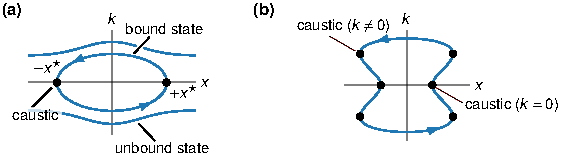
\includegraphics{localization/caustic.pdf}
  \end{center}
  \caption{%
    (a) In phase space, bound states are represented by rays in the form of closed orbits, which is analogous to that of a bound particle oscillating between two classical turning points ($\pm x^{\star}$ in the cartoon).
    Other trajectories represent unbound states.
    (b) A bound state represented by a ``peanut''-shaped orbit has six caustics.%
  }
  \label{fig:caustic}
\end{figure}

\the\textwidth

%! TEX root = thesis.tex
% vim: ft=tex et sts=2 sw=2

\chapter[Wave localization in thin elastic structures]{Wave localization in thin elastic structures\footnote{
  This chapter is an extended version of \href{https:/arxiv.org/abs/2306.07213}{M.~Mannattil and C.~D.~Santangelo, arXiv:2306.07213 [cond-mat.soft]}.
  The problem discussed in this work emerged during discussions with my coauthor.
  I was responsible for all the analytical and numerical calculations and wrote the paper taking into consideration my coauthor's comments.
}}

% This chapter is organized as follows.
% In Section~\ref{sec:wkb}, we review the semiclassical theory of wave propagation.
% We discuss wave propagation on curved rods and shells in Sections~\ref{sec:rods} and \ref{sec:shell}, respectively.
% We conclude in Section~\ref{sec:conclusion}.\\[-0.5em]

\section{Introduction}
\label{sec:introduction}

Studying the propagation of elastic waves on thin structures is of crucial importance to a variety of problems in science and engineering, with applications ranging from acoustic cloaks to negative refraction~\cite{farhat2009,craster2012,zangeneh-nejad2019}.
Of particular relevance to many of these applications are localized waves, which are time-harmonic solutions to a wave equation that remain confined to a certain region of space without the presence of a confining potential or force.
Indeed, such waves are observed in many physical systems and they are often caused by heterogeneities in the medium or the boundary.
For instance, the Helmholtz equation admits bound states in arbitrary dimensions when solved on a tubular domain, provided that the tube is not everywhere straight~\cite{goldstone1992}.
Likewise, in waveguides in the form of an elastic plate, described again by coupled Helmholtz equations, waves localize around points of maximal curvature~\cite{gridin2005}.
Bound waves of similar nature have also been predicted in waveguides in the form of rods~\cite{gridin2005a}, elastic strips with varying elastic moduli~\cite{forster2006} and thickness~\cite{postnova2008}, quantum waveguides~\cite{duclos1995}, etc.

Localized waves can also arise in elastodynamic systems described by higher-order wave equations.
In this context, \citet{scott1992} studied the localized vibrations of a musical saw---an ordinary hand saw bent into the shape of the letter \textsf{S} and playable like a musical instrument~\cite{leonard1989,stuckenbruck2016}.
More recently, \citet{shankar2022} revisited the musical saw using both experiments and theory.
Forgoing an explicit analytical computation of the mode frequencies, they argued that the bound modes that appear at the inflection point of the saw are topologically protected.
Localization of elastic waves on variably-curved shells, such as the musical saw, is not entirely surprising as it is known that curvature acts as an effective refractive index for such waves~\cite{norris1994,evans2013}.

Motivated by the above studies, in this paper, we investigate further aspects of curvature-controlled localization of waves in thin elastic structures, choosing a singly-curved shell and a curved rod as our examples.
If the structure is uncurved, there are three basic types of waves that can propagate.
Extensional waves propagate by stretching and compressing the structure, and involve only the tangential displacements ($u$ and $v$ in Fig.~\ref{fig:waves}).
Flexural waves, by contrast, propagate by bending the structure and involve only the normal displacement ($\zeta$ in Fig.~\ref{fig:waves}).
In flat plates, shear waves, which do not compress or expand the plate, and involving only the tangential displacements propagate as well~\cite{landau1986}.

The situation gets complicated when the structure is curved.
First, curvature tends to couple the tangential and normal displacements, and therefore, we can only speak of waves that are predominantly flexural or extensional or shear like.
Second, there are no universally accepted elastodynamic equations for curved structures, and in case of the rod and the shell, several choices exist~\cite{morley1961,pierce1993,doyle2021,kernes2021}.
The simplest ones, however, are almost always a set of linear partial differential equations that couple the normal and tangential displacements, the independent variables being time and the coordinates that describe the undeformed configuration of structure ($x$ and $y$ in Fig.~\ref{fig:waves}).
The physical assumptions usually made (expressed here in terms of the wave number $k$ and the structure's curvature $m$) while writing down such a set of equations are~\cite{pierce1993,norris1994,kernes2021}:
%
\begin{enumerate}
  \item The wavelength ($\sim k^{-1}$) is much larger that the thickness of the structure.
    If we work in length units such that the thickness is of order unity, we must then have $k \ll 1$.
    For bulk waves with wavelengths much smaller than the thickness (i.e., when $k \gg 1$), the structure should be treated as an infinite elastic medium~\cite{landau1986}.
  \item The radius of curvature is much larger than the thickness, so that $\abs{m} \ll 1$ (in length units such that thickness is order unity).
  \item The wavelength is smaller or of the order magnitude as the radius of curvature ($= m^{-1}$), so that $k > m$ is a safe choice (in all length units).
\end{enumerate}

Because the curvature couples the different displacement components, irrespective of the equations we use, to fully characterize wave propagation on curved structures, we have to consider multicomponent (i.e., vector) waves.
Computing the exact spectrum of a multicomponent differential operator is often difficult, unless one resorts to numerical techniques.
Indeed, for this reason, in their theoretical analyses of the musical saw, both \citet{scott1992}, and \citet{shankar2022} chose to simplify matters by analyzing flexural vibrations alone.
%
\begin{figure}
  \begin{center}
    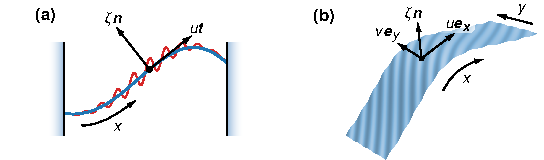
\includegraphics{localization/waves.pdf}
  \end{center}
  \caption{
    Waves can propagate on thin elastic structures such as (a) rods and (b) shells.
    The undeformed structure is parameterized by the coordinates $x$ and $y$.
    Curvature couples tangential displacements ($u$ and $v$) that stretch/shear the structure with normal displacements ($\zeta$) that bend it.
  }
  \label{fig:waves}
\end{figure}

% TODO -- previously.
As we have remarked previously, the semiclassical/WKB approximation is a widely used technique to obtain asymptotic solutions to wave problems, including those describing the elastodynamics of thin structures~\cite{pierce1970,nielsen2014,sndergaard2016,mohammed2021}.
Additionally, in wave equations supporting bound-state solutions, the semiclassical approximation allows one to extract the corresponding frequencies through quantization.
In multicomponent equations, however, subtleties can arise owing to the presence of an extra phase in the quantization rule~\cite{yabana1986,kaufman1987,littlejohn1991,littlejohn1991a}.
Recently, this phase has been shown~\cite{venaille2023} to be responsible for a spectral flow in the rotating shallow-water equations that describe oceanic waves on the Earth's surface, leading to the topological protection of equatorial waves~\cite{delplace2017}.

In this paper, we use the semiclassical approximation to study the bound-state spectrum of elastic waves in a curved rod and a singly-curved shell with a varying curvature profile.
To avoid losing the main results of the paper in a thicket of details, we summarize them here:
%
\begin{enumerate}
  \setlength\itemsep{0em}
  \item[(i)] For both the rod and the shell, independent of the boundary conditions, waves exhibit robust localization around points where the absolute curvature has a minimum.
    Wave localization induced by the presence of an inflection point in an $\mathsf{S}$-shaped musical saw~\cite{scott1992,shankar2022} is a special case of this more general observation.
    These findings also complement the prediction by \citet{mohammed2021} regarding the localization of flexural waves in a curved shell around points of maximal curvature.
  \item[(ii)] In a curved rod, only extensional waves form bound states and flexural waves always form ``unbound'' states that are spread across the rod.
  \item[(iii)] In a shell, waves of all three types can form states that are bound along the curved direction
    [$x$ in Fig.~\ref{fig:waves}(b)].
    In the frequency spectrum, flexural bound states appear first and have the lowest frequencies.
    They are then followed by shear and extensional bound states, in that order.
  \item[(iv)] For both structures, flexural waves start propagating well below the frequency of the first bound state associated with an extensional wave.
    Hence, in very long rods and shells, these bound states coexist with a near-continuum of flexural waves, forming quasi bound states in a continuum~\cite{hsu2016}.
  \item[(v)]
    Finally, both structures are described by equations for which the extra phase in the modified quantization rule vanish---something that we expect to be generically true for equations of thin-walled structures.
    This simplifies our analysis considerably and results in remarkable agreement between the quantization results and numerical experiments.
\end{enumerate}

Our findings show that waves can be robustly trapped in thin elastic structures by a simple alteration of their geometry.
This could help, for instance, in crafting better thin-plate acoustic cloaks~\cite{farhat2009}, and aid the control of noise and vibration in thin structures~\cite{mace1987,hansen2012}.
Curvature-induced localization of waves could also be used to improve the acoustic black-hole effect in thin-walled structures~\cite{lee2017,pelat2020}, which at the moment relies primarily on wave localization caused by a power-law tapered thickness profile~\cite{krylov2020}.
Finally, a singly-curved shell serves as a simple, yet effective single-mode waveguide that can steer flexural waves of specific frequencies in the uncurved direction.

%\section{Semiclassical theory of waves}
%\label{sec:wkb}

%In this section we present a quick rundown of the semiclassical approximation as applied to multicomponent waves.
%For more detailed descriptions, we refer to the book by \citet{tracy2014}.
%Consider a wave equation of the form
%%
%\begin{equation}
%  \partial_{t}^{2}\Psi(x,t) + \widehat{\mathsf{H}}\Psi(x,t) = 0,
%\end{equation}
%%
%where $\Psi(x,t)$ is an $N$-component wave field described by a one-dimensional coordinate $x$ and time $t$.
%In elastodynamics, $\Psi$ is usually composed of displacements, e.g., for the rod we have $\Psi = (\zeta, u)$, and for the shell we have $\Psi = (\zeta, u, v)$ [see Figs.~\ref{fig:waves}(a) and~\ref{fig:waves}(b)].
%Also, $\widehat{\mathsf{H}}$ is taken to be a Hermitian operator in the form of an $N\times N$ matrix, composed solely of spatial derivatives (i.e., powers of $\partial_{x}$) with time-independent coefficients.
%Assuming that the waves are time harmonic with frequency $\omega$, i.e., $\Psi(x, t) = \psi(x)e^{\pm i\omega t}$, where $\psi(x)$ is the time-independent part of the wave field, Eq.~\eqref{eq:full_wave_eq} can be recast as
%%
%\begin{equation}
%  \widehat{\mathsf{D}}\psi = 0,\quad \text{with}\enspace \widehat{\mathsf{D}} = \widehat{\mathsf{H}} - \omega^{2}\mathsf{I}_{N},
%\end{equation}
%%
%where $\mathsf{I}_{N}$ is the $N\times N$ identity matrix.
%If the coefficients of the spatial derivatives that appear in $\widehat{\mathsf{D}}$ are constants, then the eigenmodes $\psi$ are plain waves.
%In what follows we assume that these coefficients are slowly varying, with the variation controlled by a single positive parameter $\epsilon \ll 1$.
%It is useful to treat $\epsilon$ as an ordering parameter so that we can look for solutions at various orders of $\epsilon$.
%To this end, we rescale $x \to \epsilon^{-1}x$ so that a derivative $\partial_{x}$ becomes $\epsilon \partial x$.
%With analogy to quantum mechanics, this allows us to recast the derivatives in $\widehat{\mathsf{D}}$ in terms of the wave number/momentum operator $\hat{k} = -i\epsilon \partial_{x}$, with $\epsilon$ playing the role of Planck's constant.
%Since we shall be considering $\widehat{\mathsf{D}}$ in the coordinate representation, the position operator $\hat{x} = x$.

%We look for \emph{eikonal} solutions to Eq.~\eqref{eq:ev_problem} of the form $\psi(x) = A(x)e^{iS(x)/\epsilon}$, where the amplitude $A(x)$ is an $N$-component spinor with complex components, and $S(x)$ is a rapidly varying phase, playing the role of an action.
%In order to solve Eq.~\eqref{eq:ev_problem} at various orders of $\epsilon$, it is convenient to make use of Weyl calculus, which allows one to map differential operators that are functions of $\hat{x}$ and $\hat{k}$ to ordinary functions, called Weyl symbols, defined on an $x$-$k$ phase space, and vice versa~\cite{chaichian2001,cohen2012}.
%For the purposes of this paper, the following simple rules suffice to convert operators to symbols:
%%
%\begin{equation}
%  f(x) \to f(x),\enspace
%  g(\hat{k}) \to g(k),\enspace\text{and}\enspace
%  f(x)g(\hat{k}) \to f(x)g(k) + \frac{i\epsilon}{2}f'(x)g'(k) + \mathcal{O}(\epsilon^{2}).
%\end{equation}
%%
%Above, $f$ and $g$ are functions of $x$ and $\hat{k}$, with the primes denoting derivatives.

%Converting each entry of the matrix operator $\widehat{\mathsf{D}}$ into a Weyl symbol, we get the $N\times N$ dispersion matrix $\mathsf{D}$, which we express in various orders of $\epsilon$ as $\mathsf{D} = \mathsf{D}^{(0)} + \epsilon\mathsf{D}^{(1)} + \mathcal{O}(\epsilon^{2})$.
%Employing the eikonal ansatz, at $\mathcal{O}(\epsilon^{0})$, we find the matrix equation $\mathsf{D}^{(0)}A = 0$.
%To satisfy this equation, at least one of the $N$ eigenvalues of $\mathsf{D}^{(0)}$, say $\lambda(x, k;\, \omega)$, must vanish so that $\det \mathsf{D}^{(0)}(x, k; \omega) = 0$.
%A vanishing eigenvalue $\lambda$ and the associated normalized eigenvector $\tau$ describes different wave types or ``polarizations'' represented by Eq.~\eqref{eq:ev_problem}.
%By a polarization we mean a linear subspace of the total wave field that is usually of a distinct physical nature, e.g., flexural waves on a curved rod.
%Semiclassical approximation breaks down near points where more than one eigenvalues of $\mathsf{D}^{(0)}$ simultaneously vanish, precipitating an exchange of energy and mode conversion between waves of different polarizations~\cite{tracy2014}.

%In the absence of mode conversion, the vanishing eigenvalues of $\mathsf{D}^{(0)}$ also serve as the \emph{ray Hamiltonian} of waves of a specific polarization.
% This leads us to the phase-space representation of waves as rays that satisfy the Hamilton's equations
%%
%\begin{equation}
%  \dot{x} = \partial_{k} \lambda(x, k;\, \omega) = \left\{x, \lambda\right\}
%  \quad\text{and}\quad
%  \dot{k} = -\partial_{x} \lambda(x, k;\, \omega) = \left\{k, \lambda\right\},
%\end{equation}
%%
%where the overdot denotes derivatives with respect to a parameter that parameterizes the rays and $\left\{\cdot, \cdot\right\}$ is the $x$-$k$ Poisson bracket.
%Since the waves we consider propagate in a one-dimensional space, these rays are identical to the level curve defined by $\lambda(x, k; \omega) = 0$.
%%
%\begin{figure}
%  \begin{center}
%    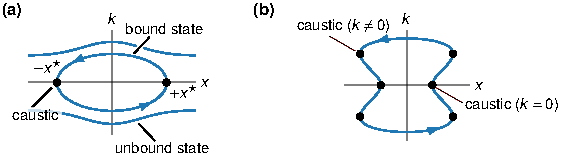
\includegraphics{localization/caustic.pdf}
%  \end{center}
%  \caption{%
%    (a) In phase space, bound states are represented by rays in the form of closed orbits, which is analogous to that of a bound particle oscillating between two classical turning points ($\pm x^{\star}$ in the cartoon).
%    Other trajectories represent unbound states.
%    (b) A bound state represented by a ``peanut''-shaped orbit has six caustics.%
%  }
%\end{figure}

%%%
%%\begin{equation}
%%\gamma_{\text{G}} = \oint \dd{\sigma}\, \dot{\gamma}_{\text{G}} = i\oint \dd{\sigma}\,\left\langle{\tau_{\alpha}}\middle|\dot{\tau}_{\alpha}\right\rangle =
%%  i\oint \dd\xi\cdot\left\langle{\tau_{\alpha}}\middle|\nabla_{\xi}\tau_{\alpha}\right\rangle,
%%\end{equation}
%%%
%%where $\xi = (x, k)$ denotes the ``parameters'' that are being varied.

%%In Appendix~\ref{app:additional_phase} we prove that $\gamma_{\text{G}}$ vanishes if the relative phases between the components of the eigenvector $\tau_{\alpha}$ are constants.
%%The second (non-geometric) phase $\gamma_{\text{NG}}$ need not vanish in such a situation, however.
%Instead of explicitly accounting for the extra phase $\gamma$ in the quantization rule, we could have diagonalized the wave equation at various orders of $\epsilon$~\cite{littlejohn1991,littlejohn1991a,weigert1993,venaille2023}.
%During such a procedure, terms proportional to $\dot{\gamma}_{\text{G}}$ and $\dot{\gamma}_{\text{NG}}$ naturally appear in the ray Hamiltonian $\lambda$ as a first-order correction.
%Despite the elegance of the method, we do not use it in our analysis.
%This is because, as we discuss in Appendix~\ref{app:additional_phase}, for both the problems we consider, the extra phases vanish.

%\section{Waves on a curved rod}
%\label{sec:rods}

%As we remarked earlier, several rod theories~\cite{chidamparam1993,walsh2000}, with varying levels of sophistication, have been written down for describing wave propagation on rods---straight or curved.
%For our purposes, a simple linear model~\cite{kernes2021} of a curved rod would do.
%This model ignores higher-order effects like torsion, cross-sectional rotation, etc., and can be viewed as the lower-dimensional analogue of the Donnell--Yu shell model~\cite{donnell1933,yu1955} that we shall later use to understand wave propagation on curved shells.

\subsection{Equations of motion and semiclassical approximation}
\label{sec:rod_equations}

Let the undeformed state of the rod be in the form of a plane curve $\bm{\sigma}: \mathcal{X} \to \mathbb{R}^{2}$, which we take to be parameterized by its arclength $x \in \mathcal{X} \subset \mathbb{R}$.
As a wave propagates along the rod, it undergoes a deformation $\bm{\sigma} \to \bm{\sigma} + \delta\bm{\sigma}$, where the displacement field $\delta\bm{\sigma}(x,t) = u(x,t)\bm{t}(x) + \zeta(x,t)\bm{n}(x)$.
Here $\bm{t} = \dd\bm{\sigma}/\dd{x}$ is the unit tangent of the undeformed rod and $\bm{n}$ is its unit normal, obtained by rotating $\bm{t}$ counter-clockwise by $\pi/2$ [see Fig.~\ref{fig:waves}(a)].
Using $\zeta$ and $u$ as the components of the wave field, and assuming the absence of external forces, the rod equations we are after is derived from the following energy functional~\cite{kernes2021}:
%
\begin{equation}
  \mathscr{U}[\zeta, u] = \int \dd{t}\,\dd{x}\,\frac{1}{2}\left\{\rho\left(\dot{u}^{2} + \dot{\zeta}^{2}\right) - E\left[\partial_{x}u - m(x)\zeta\right]^{2} - B\left(\partial_{x}^{2}\zeta\right)^{2}\right\}.
  \label{eq:rod_energy}
\end{equation}
%
Above, we have assumed that the rod is uniform with linear mass density $\rho$, with extensional stiffness $E$ and bending stiffness $B$.
Also, the signed curvature of the rod is $m(x) = \bm{n}\cdot\dd\bm{t}/\dd{x}$, which we assume to vary with the arclength $x$.
With these identifications, we can delineate the bending and stretching contributions to the energy.%
\footnote{%
  The stretching contribution to the energy is approximated by taking the usual one-dimensional strain $\partial_{x}u$ and adding to it the circumferential strain, which for a (convex) differential element of the rod with angular width $\delta\theta$ and radius $r = -m^{-1}$ is roughly $[(r + \zeta)\delta{\theta} - r\delta\theta]/(r\delta\theta) = -m\zeta$~\cite{donnell1933}.
The bending energy, on the other hand, is the usual Euler--Bernoulli bending energy, without any additional curvature-dependent corrections.
See Section~\ref{sec:rod_ho} for a rod model that includes additional corrections to the bending energy.}
Upon varying the energy functional~$\mathscr{U}$, we get the dynamic rod equations
%
\begin{subequations}
\begin{align}
  \label{eq:rod_flex}
  \rho\partial_{t}^{2}\zeta &= -B\partial_{x}^{4}\zeta - Em(x)\left[m(x)\zeta - \partial_{x}u\right],\\
  \rho\partial_{t}^{2}u &= -E\left\{\partial_{x}\left[m(x)\zeta\right] - \partial_{x}^{2}u\right\}.
  \label{eq:rod_ext}
\end{align}
\end{subequations}
%
When the curvature $m = 0$, Eq.~\eqref{eq:rod_flex} reduces to the dynamic Euler--Bernoulli equation representing purely transverse flexural waves that propagate by bending the rod.
In the same limit, Eq.~\eqref{eq:rod_ext} characterizes extensional waves that propagate longitudinally by stretching the rod.
When curvature is nonzero, which is the case we want to analyze, the components $\zeta$ and $u$ remain coupled.

In terms of the rod's Young's modulus $Y$, cross-sectional area $A$, and its second moment of area $I$, the extensional and bending stiffnesses are $E = YA$ and $B = YI$, respectively.
If the rod's cross-sectional ``thickness'' is $h$, then $A \sim h^2$ and $I \sim h^{4}$.
This gives a natural length unit $\ell = \sqrt{B/E} \sim h$ and a time unit $\sqrt{B\rho}/E$ that can be used to conveniently nondimensionalize the rod equations.
Noting that under a change of length units the curvature transforms as $m(x) \to \ell^{-1}m(x)$, we arrive at the nondimensional form of the rod equations, which in matrix form reads [cf. Eq.~\eqref{eq:full_wave_eq}]
%
\begin{equation}
\partial_{t}^{2}
\begin{pmatrix}
  \zeta\\
  u
\end{pmatrix} +
\widehat{\mathsf{H}}
\begin{pmatrix}
  \zeta\\
  u
\end{pmatrix} = 0,
\enspace
\text{where}
\enspace
\widehat{\mathsf{H}}
=
\begin{pmatrix}
  \partial^{4}_{x} + m^{2}(x) & -m(x)\partial_{x}\\
  m(x)\partial_{x} + m'(x) & -\partial^{2}_{x}
\end{pmatrix}.
\label{eq:rod}
\end{equation}
%
Although this is a rather simple set of coupled equations involving the curvature $m(x)$ as the only parameter, a nonuniform $m(x)$ makes obtaining a general solution difficult.

To employ the semiclassical approximation for solving Eq.~\eqref{eq:rod}, we assume that the curvature is a slowly varying function of the form $m(\epsilon x)$.
Here $0 < \epsilon \ll 1$ is a small dimensionless parameter that controls the slowness of the variation.
Because the length unit $\ell$ we chose for nondimensionalizing the arclength $x$ is proportional to the thickness, physically speaking, here we are assuming that the length scale over which the curvature varies significantly is much larger that the thickness of the rod.
%(The actual length scale over which the curvature varies significantly is $\epsilon^{-1}\ell$.)
Next, we do a final change of variables $x \to \epsilon^{-1}x$ in Eq.~\eqref{eq:rod} so that $m(\epsilon x) \to m(x)$ and all spatial derivatives get multiplied by $\epsilon$.
For the eigenvalue problem with $\widehat{\mathsf{D}} = \widehat{\mathsf{H}} - \omega^{2}\mathsf{I}_{2}$, this gives us
%
\begin{equation}
 \widehat{\mathsf{D}} =
 \begin{pmatrix}
    \epsilon^{4}\partial^{4}_{x} + m^{2}(x) - \omega^{2} & -m(x)\epsilon\partial_{x}\\
    m(x)\epsilon\partial_{x} + \epsilon m'(x) & -\epsilon^{2}\partial^{2}_{x} - \omega^{2}
 \end{pmatrix}
=
 \begin{pmatrix}
   \hat{k}^{4} + m^{2}(x) -\omega^{2} & -i m(x)\hat{k}\\
    im(x)\hat{k} + \epsilon m'(x) & \hat{k}^{2} - \omega^{2}
\end{pmatrix}.
\label{eq:filwaveop}
\end{equation}
%
In the final step above, we have set $\epsilon\partial_{x} \to i\hat{k}$, with $\hat{k}$ being the momentum operator.
Using the rules in Eq.~\eqref{eq:weylrules} we can easily write down the Weyl symbol $\mathsf{D}$ for the operator in Eq.~\eqref{eq:filwaveop} as
$\mathsf{D} = \mathsf{D}^{(0)} + \epsilon\mathsf{D}^{(1)}$, where
%
\begin{equation}
\mathsf{D}^{(0)} =
 \begin{pmatrix}
    {k}^{4} + m^{2}(x) - \omega^{2} & -i m(x){k}\\
    im(x){k} & {k}^{2} - \omega^{2}
\end{pmatrix}
\enspace \text{and} \enspace
\mathsf{D}^{(1)} =
\frac{1}{2}
\begin{pmatrix}
    0 & m'(x)\\
    m'(x) & 0
\end{pmatrix}.
\label{eq:rod_D}
\end{equation}

The two eigenvalues of the dispersion matrix $\mathsf{D}^{(0)}$, representing waves of two different polarizations, are
%
\begin{equation}
  \lambda_{\pm} = \frac{1}{2}\left\{k^{2} + k^{4} + m^{2}(x) \pm \sqrt{\left[k^{2} - k^{4} - m^{2}(x)\right]^{2} + 4k^{2}m^{2}(x)}\right\} - \omega^{2}.
  \label{eq:rod_ham}
\end{equation}
%
For a given $\omega$, we have $\lambda_{+}(x, k;\, \omega) \geq \lambda_{-}(x, k;\, \omega)$ for all values of $x$ and $k$.
Mode conversion between the two polarizations ensues near points where $\lambda_{+}(x, k;\, \omega) = \lambda_{-}(x, k;\, \omega)$, and the semiclassical approximation breaks down.
But from Eq.~\eqref{eq:rod_ham}, we see that $\lambda_{+} = \lambda_{-}$ only when the discriminant in Eq.~\eqref{eq:rod_ham} vanishes, which happens only when $m(x)$ is zero, and $k = \pm 1$ or $k = 0$.
As we discussed in Section~\ref{sec:introduction}, the rod equations are only applicable for short waves whose wavelength is much longer than the thickness, which translates to the requirement $0 \ll \abs{k} \ll 1$.
Hence, mode-conversion points with $k = \pm 1$ or $k = 0$, lie well beyond the range of applicability of these equations.
For this reason, we ignore mode-conversion issues and assume that $\lambda_{+} \neq \lambda_{-}$ throughout our analysis.
Before moving on, it is useful to first analyze the propagation of waves on a rod of constant curvature.

\subsection{Rods of constant curvature}

First we analyze the case where the curvature is zero, i.e., when the rod is straight.
In the limit of vanishing curvature $m$, we should recover the dispersion relations $\omega(k)$ for plane waves propagating on a straight rod from $\lambda_{\pm}$.
On setting $m = 0$ and noting that $\abs{k} \ll 1$, we see that $\lambda_{+} = 0$ gives us the linear dispersion relation $\omega = k$, representing extensional waves propagating on a straight rod.
Meanwhile, when $m = 0$, we find that $\lambda_{-} = 0$ gives us the quadratic dispersion relation $\omega = k^{2}$ of flexural waves on a straight rod.
%For this reason, from now on we shall call waves represented by $\lambda_{-}$ as flexurally polarized waves and those represent by $\lambda_{+}$ as extensionally polarized waves.

For nonzero, but constant curvature, the rod forms part of a ring.
If the curvature is sufficiently weak, we expect the eigenvalue $\lambda_{+}$ to continue to represent predominantly extensional waves and $\lambda_{-}$ to represent predominantly flexural waves.
To verify this, we expand $\lambda_{\pm}$ in powers of $m^{2}$ and drop powers of $k$ in comparison to unity to find
%
\begin{equation}
  \lambda_{+} = k^{2} + m^{2} - \omega^{2} + \mathcal{O}(m^{4})
  \quad\text{and}\quad
  \lambda_{-} = k^{4} - k^{2}m^{2} - \omega^{2} + \mathcal{O}(m^{4})
  \qquad{(k \gg m)}.
  \label{eq:rod_kgm}
\end{equation}
%
Clearly, the above expansions can only be valid when the $\mathcal{O}(m^{2})$ correction terms are less than the lowest-order terms, which is true only when $k \gg m$.
In this limit we have $\lambda_{+} \sim k^{2} - \omega^{2}$ and $\lambda_{-} \sim k^{4} - \omega^{2}$, confirming our expectation.

We next look at the case where both $k$ and $m$ are small,%
\footnote{%
  We consider this limit to analyze the behavior of the waves close to a classical turning point where $k = 0$.
  The wave decays beyond a turning point and it never gets a chance to complete a full-wavelength oscillation with $k \ll m$, so that the short wavelength assumption is not violated.
}
but with $k \ll m$.
To this end, we expand $\lambda_{\pm}$ in powers of $km^{-1}$ to find
%
\begin{equation}
  \lambda_{+} = k^{2} + m^{2} - \omega^{2} + \mathcal{O}(k^{4})
  \quad\text{and}\quad
  \lambda_{-} = \frac{k^{6}}{m^{2}}\left[1 + \mathcal{O}\left(\frac{k^{2}}{m^{2}}\right)\right] - \omega^{2}
  \qquad{(k \ll m)}.
  \label{eq:rod_klm}
\end{equation}
%
Dispersion relations obtained from setting $\lambda_{\pm} = 0$ above show significant deviation from those of a straight rod and we expect the waves of both polarizations to result in bending and stretching of the rod.
For the same reason, we expect both these waves to have both longitudinal and transverse characteristics.
Despite this, for the sake of simplicity and identification, we shall continue to call waves represented by $\lambda_{+}$ as extensional waves and those represented by $\lambda_{-}$ as flexural waves.

Bending of the rod is associated with normal component $\zeta$ and stretching with tangential component $u$.
To better understand how the two components contribute to the wave field in the presence of curvature, we define the amplitude ratio
%
\begin{equation}
  \mathscr{R} = \frac{\abs{\zeta}}{\abs{\zeta} + \abs{u}}.
  \label{eq:rod_ratio}
\end{equation}
%
With the above definition, for purely transverse and longitudinal waves $\mathscr{R} = 1$ and $\mathscr{R} = 0$, respectively.
In the eikonal ansatz, at the lowest order, the wave field $\psi = (\zeta, u)$ is proportional to the eigenvectors $\tau_{\pm}$ of $\mathsf{D}^{(0)}$ so that $\zeta \sim \tau_{\pm,1}$ and $u \sim \tau_{\pm,2}$.
Making use of Eqs.~\eqref{eq:rod_kgm} and \eqref{eq:rod_klm}, to the lowest order in $k$ and $m$, the eigenvectors $\tau_{\pm}$ are
%
\begin{equation}
  \tau_{+} \sim \left(m,\enspace ik\right)
  \quad\text{and}\quad
  \tau_{-} \sim \left(ik,\enspace m\right),
  \label{eq:rod_tau}
\end{equation}
%
so that the asymptotic amplitude ratios for the two wave polarizations become $\mathscr{R}_{+} \sim \abs{m}/(\abs{m} + \abs{k})$ and $\mathscr{R}_{-} \sim \abs{k}/(\abs{m} + \abs{k})$.
For $m = 0$, we know that extensional waves become entirely longitudinal, and as expected the corresponding amplitude ratio $\mathscr{R}_{+} = 0$.
In same limit, flexural waves become entirely transverse as indicated by $\mathscr{R}_{-} = 1$.
However, for small values of $k$ with $k \ll m$ we see that $\mathscr{R}_{+} \to 1$ and $\mathscr{R}_{-} \to 0$.
In other words, in the limit $k \ll m$, waves of the two polarizations would switch their nature from being predominantly longitudinal to being predominantly transverse, and vice versa.

\subsection{Rods with varying curvature}

For illustrative purposes, we consider rods of two curvature profiles $m_{1}(x)$ and $m_{2}(x)$, defined~by
%
\begin{equation}
  m_{1}(x) = b\tanh(\epsilon x)
  \quad\text{and}\quad
  m_{2}(x) = b - \left(b - a\right)\sech(\epsilon x),
  \label{eq:rod_curv}
\end{equation}
%
which we will informally call tanh- and sech-type curvature profiles, respectively.
Above, $b$ and $a$ are positive constants such that $a < b$ and the parameter $\epsilon$ controls the slowness of variation of the curvatures.
A rod with a tanh-type curvature profile $m_{1}(x)$ possesses an inflection point at $x=0$ where the curvature vanishes, and the curvature asymptotes to $\pm b$ as $x\to \pm\infty$ [see Figs.~\ref{fig:rod_bound}(a) and~\ref{fig:rod_bound}(b)].
On the other hand, a rod with a sech-type curvature profile $m_{2}(x)$ remains concave for all $x$, with the curvature acquiring its minimum value of $a$ at $x = 0$ and asymptoting to $b$ as $x\to\pm\infty$ [see Figs.~\ref{fig:rod_bound}(c) and~\ref{fig:rod_bound}(d)].
For the purpose of illustrating our results, we take $b = 0.1$ and $a = 0.01$, so that the smallest ratio between the radius of curvature and thickness is $\mathcal{O}(10)$.
Although such a ratio is comparatively smaller than typical experimental values, it would give us a clearer picture of the effects of a varying curvature profile.
We also set $\epsilon = 0.01$, but as we rescale $x \to \epsilon^{-1}x$, the parameter $\epsilon$ does not always explicitly appear in our discussions.
Note also that the numerical values of the local wave number $k$ is unaffected by this rescaling.

For a varying curvature profile, we find the rays for both polarizations by integrating the corresponding Hamilton's equations given by
%
\begin{equation}
  \begin{alignedat}{2}
      \dot{x} &= \frac{\partial \lambda_{\pm}}{\partial k} &&= k\left\{2k^{2} + 1 \pm \frac{(2k^{2} + 1)\left[k^{2} + k^{4} + m^{2}(x)\right] - 6k^{4}}{\sqrt{\left[k^{2}-k^{4}-m^{2}(x)\right]^{2} + 4k^{2}m^{2}(x)}}\right\};\\
      \dot{k} &= -\frac{\partial \lambda_{\pm}}{\partial x} &&= -\frac{1}{2}\left[m^{2}(x)\right]'\left\{1 \pm \frac{k^{2} + k^{4} + m^{2}(x)}{\sqrt{\left[k^{2}-k^{4}-m^{2}(x)\right]^{2} + 4k^{2}m^{2}(x)}}\right\}.
  \end{alignedat}
  \label{eq:rod_hamiltonian}
\end{equation}
%
\begin{figure}
  \begin{center}
    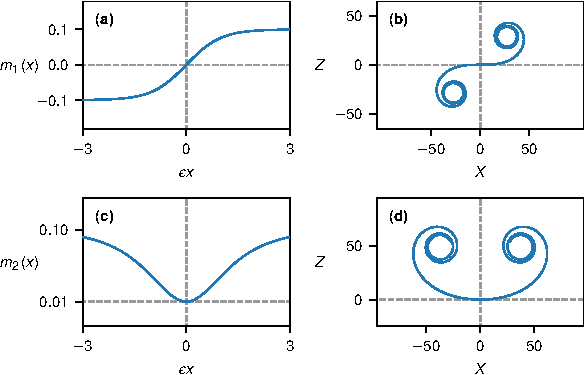
\includegraphics{localization/rod_profile.pdf}
  \end{center}
  \caption{%
    (a) Tanh-type curvature profile $m_{1}(x)$ with an inflection point at $x = 0$ and (b) the corresponding shape of the rod in Cartesian space with coordinates $X$ and $Z$.
    (c) Sech-type curvature profile $m_{2}(x)$ with no inflection point and (d) the corresponding shape of the rod.
    For both curvature types, as the arclength $x \to \pm\infty$, the rod becomes part of a circle.
    In all figures $a = 0.01$, $b = 0.1$, and $\epsilon = 0.01$.
  }
  \label{fig:rod_profile}
\end{figure}

\subsection{Extensional waves}
\label{sec:extensional}

We first discuss how a varying curvature profile affects extensional waves in a rod.
In Section~\ref{sec:extensional_limit} we present an alternative approach, where we analyze the extensional limit of the rod equations and show that extensional waves form bound states.
The purpose here, however, is to understand this using a semiclassical perspective, which will serve as a basis for understanding the variably-curved shell.

As we discussed previously, extensional waves are to be associated with the ray Hamiltonian $\lambda_{+}$.
Without loss of generality, let $x = 0$ be a point where $m^{2}(x)$ has a local extremum, so that its derivative $[m^{2}(x)]'\big|_{x=0} = 0$ and the origin $(0, 0)$ becomes a fixed point of the Hamilton's equation in Eq.~\eqref{eq:rod_hamiltonian} for $\lambda_{+}$.
Since Eq.~\eqref{eq:rod_hamiltonian} is a Hamiltonian system, the origin becomes a nonlinear center or a saddle depending on whether the Hamiltonian $\lambda_{+}(x, k)$, viewed as a function of $x$ and $k$, has an extremum or a saddle there~\cite{strogatz1994,jordan2007}.
For the present problem, we find two situations%
\footnote{We can also infer this from the sign of the Hessian determinant of $\lambda_{+}$ at $(0, 0)$ given by $\det \nabla\nabla \lambda_{+}\big|_{x=0,k=0} = 2(m^{2})''\big|_{x=0}$, provided that $(m^{2})'' \neq 0$ so that the origin is a nondegenerate fixed point with $\det\nabla\nabla\lambda_{+} \neq 0$.}
depending on the behavior of $m^{2}(x)$ at $x = 0$.
%
\begin{enumerate}
    \item[(i)]
  \emph{$m^{2}$ has a nonzero maximum at $x = 0$.\enspace}
  Then, for any point $x$ sufficiently close to $0$, we have $m^{2}(x) < m^{2}(0) = \lambda_{+}(0, 0)$.
  We also see that $\lambda_{+}(x, 0) - \lambda_{+}(0, 0) < 0$, whereas $\lambda_{+}(0, k) - \lambda_{+}(0, 0) > 0$.
  In other words, if we move along the $x$ axis from the origin $(0, 0)$, the value of $\lambda_{+}(x, k)$ decreases, whereas moving along the $k$ axis increases its value, showing that the origin becomes a saddle point.

  \item[(ii)] \emph{$m^{2}$ has a minimum at $x = 0$.\enspace}
    At any point $(x, k)$ sufficiently close to $(0, 0)$, we have $m^{2}(x) > m^{2}(0)$.
    Then, using basic inequality arguments, $\lambda_{+}(x, k) - \lambda_{+}(0, 0) > 0$, showing that $\lambda_{+}$ has a minimum at the origin, which means that it becomes a nonlinear center.
\end{enumerate}
%
As the extrema of $m^{2}(x)$ are identical to the extrema of the absolute curvature $\abs{m(x)}$, we can summarize as follows: points where the absolute curvature has a minimum become nonlinear centers of the ray equations associated with $\lambda_{+}$, and points where the absolute curvature has a maximum become saddles.
Therefore, we expect extensional waves to get trapped only around points where the absolute curvature has a minimum.
%
\begin{figure}
  \begin{center}
    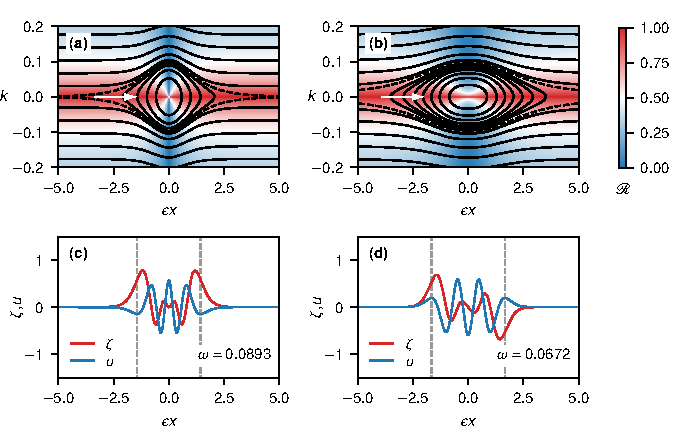
\includegraphics{localization/rod_bound.pdf}
  \end{center}
  \caption{%
    Ray trajectories for extensional waves on a rod with (a) tanh-type curvature profile $m_{1}(x)$ and (b) sech-type curvature profile $m_{2}(x)$, with the phase portraits color coded using the amplitude ratio $\mathscr{R}$ defined in Eq.~\eqref{eq:rod_ratio}.
    The white arrows in (a) and (b) indicate rays of the same frequency as the two bound states in (c) and (d).
    The grey vertical lines in (c) and (d) indicate the locations of the classical turning points.
  }
  \label{fig:rod_bound}
\end{figure}

The black curves in Figs.~\ref{fig:rod_bound}(a) and~\ref{fig:rod_bound}(b) show the extensional rays for the two curvature profiles.
Each ray is a level curve defined by $\lambda_{+}(x, k; \omega) = 0$ for a specific $\omega$.
Since $\lambda_{+}$ is invariant with respect to reflection about the $x$ and $k$ axes, the ray trajectories also share the same reflection symmetry.
For both curvature types, there are three fixed points: the origin $(0, 0)$ and $(\pm\infty, 0)$.
The fixed points at $(\pm\infty, 0)$ are saddles since $m^{2}(x)$ achieves its maximum there.
Two heteroclinic orbits, shown as black dashed curves, connect the fixed points at $(\pm\infty, 0)$.
% The origin is always a nondegenerate fixed point for a tanh-type curvature profile since $[m_{1}^{2}(x)]''\big|_{x=0} = 2b^{2}$.
% For the sech-type curvature profile, the origin is a nondegenerate fixed point only when $a$ is nonzero so that $[m_{2}^{2}(x)]''\big|_{x=0} = 2a(b - a) > 0$.
As per our analysis, the origin is always a center as $m^{2}(x)$ achieves a minimum there for both curvature types.
Close to the origin, the rays appear in form of closed orbits indicating bound states.

Before we present some example results, it is useful to analyze the parity of the bound states.
If $\psi(x) = \left[\zeta(x), u(x)\right]$ is a bound state, then it is easy to check that for an odd curvature profile $m(x)$ with $m(-x) = m(x)$, the eigenmode $\psi(-x) = \left[\zeta(-x), u(-x)\right]$ is also a bound state satisfying the rod equations, Eq.~\eqref{eq:rod}, with the boundary conditions $\psi(\pm\infty) = 0$.
Assuming nondegeneracy in the eigenmodes, we must then have $\left[\zeta(x), u(x)\right] = \pm\left[\zeta(-x), u(-x)\right]$, which means that for an odd $m(x)$, the components $\zeta(x)$ and $u(x)$ must have the same parity, i.e., they are either both odd or both even.%
\footnote{%
  More quantum mechanically, this can be shown by considering the commutation of $\widehat{\mathsf{D}}$ with the operators $\widehat{\mathsf{P}}_{\pm} = \diag\left(\widehat{\pi}, \pm\widehat{\pi}\right)$, where $\widehat{\pi}$ is the usual parity operator~\cite{cohen-tannoudji2019}.
  Clearly, $\widehat{\mathsf{P}}_{\pm}\Psi(x) = \left[\zeta(-x), \pm u(-x)\right]$ so that
  the eigenstates of $\widehat{\mathsf{P}}_{+}$ always have $\zeta(x)$ and $u(x)$ of the same parity, whereas the eigenstates of $\widehat{\mathsf{P}}_{-}$ always have $\zeta(x)$ and $u(x)$ of different parity.
  Furthermore, for odd and even $m(x)$, we can show that $\widehat{\mathsf{D}}$ commutes with $\widehat{\mathsf{P}}_{+}$ and $\widehat{\mathsf{P}}_{-}$, respectively.
  As commuting operators share the same eigenstates (assuming nondegeneracy), this proves the claim made above.%
}
For an even $m(x)$, however, we find that bound-state solutions must satisfy $\left[\zeta(x), u(x)\right] = \pm\left[\zeta(-x), -u(-x)\right]$, showing that the components $\zeta(x)$ and $u(x)$ always have different parity.
In Figs.~\ref{fig:rod_bound}(c) and~\ref{fig:rod_bound}(d) we show two example bound states obtained by solving the rod equations numerically (see Appendix \ref{app:numerical} for details) and depicting both components of the wave field $\psi$.
Consistent with our analysis, the example bound state of the tanh-type curvature profile has even $\zeta(x)$ and $u(x)$.
Likewise, for the example bound state of the sech-type curvature profile, $\zeta(x)$ is odd and $u(x)$ is even.

Clearly, the displacement fields of the bound states of both curvature profiles show a significant presence of both normal and tangential components.
To understand this better, consider again the phase portraits in Fig.~\ref{fig:rod_bound}(a) and \ref{fig:rod_bound}(b), which have been color coded using the amplitude ratio $\mathscr{R}$ defined in Eq.~\eqref{eq:rod_ratio}, and computed%
\footnote{Note that we are using the exact expression for $\tau_{+}$ and not the approximate expression in Eq.~\eqref{eq:rod_tau} to find $\mathscr{R}$.  Using the approximate expression would also result in nearly similar results.}
from the components of the polarization vector $\tau_{+}$.
The closed orbits corresponding to the example bound states have been marked with white arrows in these phase portraits.
Starting at the $k$ axis, if we move along a closed orbit towards one of its turning points, we see that $\mathscr{R}$ changes from $0$ to $1$, indicating that the wave acquires a strong normal component, which is what we see from the example bound states.

The existence of the bound states can also be intuitively understood from the dispersion relations for extensional waves.
From Eq.~\eqref{eq:rod_ham}, we see that at $k = 0$, the dispersion curve given by $\lambda_{+} = 0$ has a nonzero gap and a cut-on frequency%
\footnote{Incidentally, this cut-on frequency is the ring frequency of extensional waves, i.e., when the wavelength is equal to the circumference of a ring of radius $m^{-1}$~\cite{walsh2000}.}
of $\omega_{\text{cut-on}}^{2} = m^{2}$.
For waves with $\omega < \omega_{\text{cut-on}}$, the wave number $k$ is always complex, preventing the wave from being able to propagate and the wave decays.
Now, as an extensional wave enters a region of high curvature from a region of low curvature, the local cut-on frequency increases.
This means that, at some point, the frequency of the wave would fall below the local cut-on frequency, and the wave gets reflected creating a bound state.
As the cut-on frequency depends only on the magnitude of the curvature, and not its sign, bound states do not require the presence of an inflection point---an observation that was also made by \citet{scott1992} while analyzing the musical saw.
%
\begin{figure}
  \begin{center}
    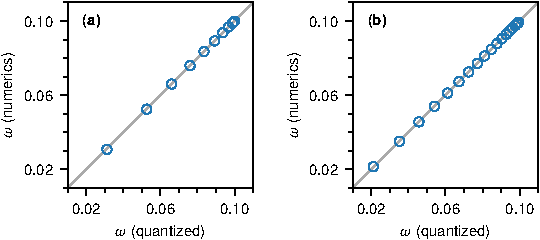
\includegraphics{localization/rod_wkb.pdf}
  \end{center}
  \caption{
    Bound-state frequencies obtained from numerics compared to that obtained through quantization for a rod with (a) tanh-type curvature profile and (b) sech-type curvature profile.
    In both plots, the gray guide line in the background represents $\omega$ (numerics) = $\omega$ (quantized).
  }
  \label{fig:rod_wkb}
\end{figure}

\subsubsection*{Quantization and bound states}

In order to evaluate the action in the quantization condition, Eq.~\eqref{eq:quantization}, in principle, we should express $k$ in terms of $x$ from $\lambda_{+}(x, k; \omega) = 0$.
This proves to be difficult as $k$ would then have to be obtained as the root of a sixth-order polynomial.
Instead, as described in Appendix~\ref{app:numerical}, we compute the action by numerically integrating $k(x)$ between the classical turning points $\pm x^{\star}$.
Setting $k = 0$ in $\lambda_{+}(x, k; \omega) = 0$, we see that these points are implicitly given by the equation $m^{2}(x^{\star}) = \omega^{2}$.
To quantize the bound orbits, we also need the Keller--Maslov index, which is $\alpha = 2$ as the orbits are topologically equivalent to a circle.
Now, note that the off-diagonal operators of the matrix $\widehat{\mathsf{D}}$ in the rod equations, Eq.~\eqref{eq:rod}, are composed only of odd derivatives.
In Appendix~\ref{app:additional_phase}, we show that the additional phase $\gamma$ in Eq.~\eqref{eq:quantization}, vanishes for any operator of this form, enabling us to find the quantized frequencies without additional difficulty.
A comparison between the numerically obtained bound-state frequencies and those obtained through quantization (Fig.~\ref{fig:rod_wkb}) shows excellent agreement between the two.
Furthermore, these frequencies are independent of the boundary conditions chosen to solve the rod equations, showing the robustness of the bound states.

Instead of computing the action by quadrature, we could have extracted $k(x)$ from the approximate expression for $\lambda_{+}$ [see Eqs.~\eqref{eq:rod_kgm} and \eqref{eq:rod_klm}], which gives $k(x) \approx \pm\sqrt{\omega^{2} - m(x)^{2}}$.
This expression can be used, for instance, to estimate the maximum number of bound states $n_{\text{max}}$ for the two curvature profiles.
The largest frequency for which we see an extensional bound state is $\omega = b$.
As shown in Figs.~\ref{fig:rod_bound}(a) and~\ref{fig:rod_bound}(b), the rays corresponding to this frequency form two heteroclinic orbits connecting the classical turning points at $x = \pm \infty$.
Computing the area inside these orbits, we find
%
\begin{equation}
  n_{\text{max}} \approx \frac{1}{\pi\epsilon}\int_{-\infty}^{+\infty} \dd{x}\,k(x) =
  \begin{dcases}
    b/\epsilon & \text{(tanh type)},\\
    \bar{b}/\epsilon + \mathcal{O}(a/\epsilon) & \text{(sech type)}.
  \end{dcases}
  \label{eq:rod_maxb}
\end{equation}
%
Here, $\bar{b} = \pi^{-1}b\int_{-\infty}^{\infty}\dd{x}\,\sech{x}\sqrt{2\cosh{x} - 1} \approx 2b$.
Therefore, we expect an infinitely long rod with a sech-type curvature profile to support twice as many bound states as a rod with a tanh-type curvature profile.
A similar expression for $n_\text{max}$ is also derived in Appendix~\ref{sec:extensional_limit} where we directly consider the extensional limit of the rod equations, and find the quantized frequencies as well as the bound modes.

For the values $b = 0.1$ and $\epsilon = 0.01$ we use in our examples, Eq.~\eqref{eq:rod_maxb} predicts a maximum of 10 bound states for a tanh-type rod and 20 bound states for a sech-type rod.
This prediction is consistent with our numerical experiments with a finite-sized rod, where we find a total of 10 and 18 bound states for the two curvature profiles.
Despite this, we only expect a small number of extensional bound states in actual experiments with curved rods, where we expect the finiteness of the rod to become more important.
For one thing, as the arc length $x \to \pm\infty$, self intersection is inevitable for both sech- and tanh-type rods having a nonzero thickness (see Fig.~\ref{fig:rod_profile}).
(Self-intersection effects, however, can be ameliorated if we allow for small motions of the rod perpendicular to the plane containing it.)
Furthermore, as the turning points of the higher-frequency bound states are far apart, they do not always appear to be spatially localized, even though they decay exponentially as $x \to \pm\infty$.
%
\begin{figure}
  \begin{center}
    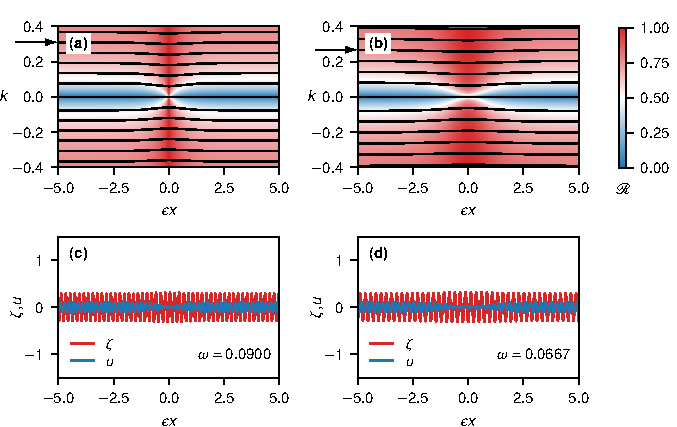
\includegraphics{localization/rod_extended.pdf}
  \end{center}
  \caption{%
    Ray trajectories for flexural waves on a rod with (a) tanh-type curvature profile $m_{1}(x)$ and (b) sech-type curvature profile $m_{2}(x)$, with the phase portraits color coded using the ratio $\mathscr{R}$ defined in Eq.~\eqref{eq:rod_ratio}.
    The black arrows in (a) and (b) indicate rays of the same frequency as the two eigenmodes in figures (c) and (d).
  }
  \label{fig:rod_extended}
\end{figure}

\subsection{Flexural waves}

Flexural waves are associated with the ray Hamiltonian $\lambda_{-}$ and from the corresponding Hamilton's equations in Eq.~\eqref{eq:rod_hamiltonian}, we see that the derivatives $\dot{x}$ and $\dot{k}$ vanish everywhere on the $x$ axis.
Since there are no isolated fixed points anywhere on the $x$ axis for these rays, we do not expect flexural waves to form bound states.
This is confirmed by the phase portraits in Figs.~\ref{fig:rod_extended}(a) and~\ref{fig:rod_extended}(b).
Like rays of extensional waves, the rays of flexural waves are also invariant under reflection about the $x$ and $k$ axes because $\lambda_{-}$ possesses the same symmetry.
Two unbound flexural eigenmodes obtained numerically are displayed in Figs.~\ref{fig:rod_extended}(c) and~\ref{fig:rod_extended}(d).
Rays corresponding to these modes have been marked by black arrows in Figs.~\ref{fig:rod_extended}(a) and~\ref{fig:rod_extended}(b).
Although the normal component $\zeta$ dominates in these modes, they acquire a significant tangential component with increasing curvature, which we also see from the color coding of the phase portraits.

Although the frequencies of the extensional bound states in Figs.~\ref{fig:rod_bound}(c) and~\ref{fig:rod_bound}(d) and the flexural eigenmodes in \ref{fig:rod_extended}(c) and~\ref{fig:rod_extended}(d) are rather close, the mode profiles differ significantly in appearance.
Also, the frequencies of the flexural eigenmodes depend on the specific boundary conditions chosen and other physical parameters, e.g., the total length of the rod.
When the rod length increases, we expect flexural waves to form a near continuum in the frequency spectrum, whereas the frequencies of the extensional bound states would continue to be determined by the quantization condition, Eq.~\eqref{eq:quantization}.
Setting $\lambda_{-} = 0$ and putting $k = 0$ in Eq.~\eqref{eq:rod_ham}, we also see that flexural waves in a rod are gapless and start propagating well below the first bound extensional state.
In this sense, in very long rods, extensional bound states appear as quasi-bound states in a continuum of flexural waves.

\section{Extensional limit of the rod equations}
\label{sec:extensional_limit}

We define the extensional limit of the rod equations as the limit in which the average bending energy of a deformed rod is considerably smaller than its stretching energy.
The bending energy in the rod model we use is proportional to $(\partial_{x}^{2} \zeta)^{2}$ [see Eq.~\eqref{eq:rod_energy}], which gives rise to the fourth-order derivative $\partial_x^{4}\zeta$ in the rod equations, Eq.~\eqref{eq:rod}.
Neglecting this term and Fourier transforming in time, we find the extensional limit of the rod equations, which take the form
%
\begin{subequations}
  \begin{align}
  \label{eq:rod_ext1}
  m(x)\left[m(x)\zeta(x) - \partial_{x}u(x)\right] &= \omega^{2}\zeta(x),\\
  \partial_{x}\left[m(x)\zeta(x) - \partial_{x}u(x)\right] &= \omega^{2}u(x).
  \label{eq:rod_ext2}
  \end{align}
\end{subequations}
%
The above equations possess a soft-mode solution with $\omega = 0$ satisfying $m(x)\zeta(x) = \partial_{x}u(x)$, which corresponds to all linear isometries that do not stretch the rod to the lowest order.
%
\begin{figure}
  \begin{center}
    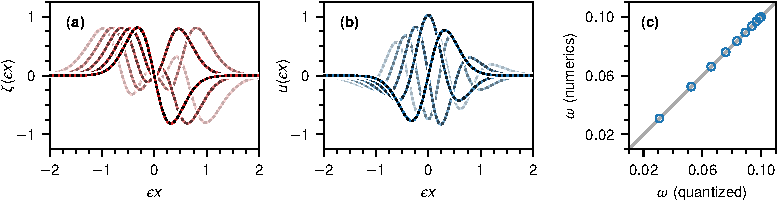
\includegraphics{localization/rod_poschl.pdf}
  \end{center}
  \caption{%
    The first five extensional bound states of a rod with a tanh-type curvature profile showing (a) the normal component $\zeta(x)$ and (b) the tangential component $u(x)$, with lighter curves depicting higher-frequency states.
    The dashed black curves in (a) and (b) represent the solutions in Eq.~\eqref{eq:poschl}.
    (c) Comparison between the bound-state frequencies $\omega$ obtained through quantization, and those from numerics [cf.~Fig.~\ref{fig:rod_wkb}(a)].
  }
  \label{fig:poschl}
\end{figure}

We now look for bound-state solutions of Eqs.~\eqref{eq:rod_ext1} and \eqref{eq:rod_ext2} satisfying $\zeta(\pm\infty) = u(\pm\infty) = 0$ with vanishing derivatives at $x = \pm\infty$.
Let us additionally assume that the longitudinal component $u(x) = \partial_{x}\phi(x)$, where $\phi(x)$ is an unknown differentiable function satisfying%
\footnote{Assuming $\phi(\pm\infty) = 0$ does not result in any loss in generality.
Without this assumption, on integrating Eq.~\eqref{eq:rod_ext2} we see that $\phi(\pm\infty) = C$ (constant).
We then obtain Eq.~\eqref{eq:schrodinger} in terms of $\widetilde{\phi}(x) = \phi(x) - C$ with $\zeta = m\widetilde{\phi}$, so that we can work in terms of $\widetilde{\phi}$ alone, which is equivalent to setting $C = 0$.}
$\phi(\pm\infty) = 0$.
Equation~\eqref{eq:rod_ext2} then becomes a total derivative, which on integration yields
%
\begin{equation}
  m(x)\zeta(x) = \partial_{x}^{2}\phi(x) + \omega^{2}\phi(x).
\end{equation}
%
Putting the above equation in Eq.~\eqref{eq:rod_ext1} and ignoring the soft-mode solution with $\omega = 0$, we see that $\zeta(x) = m(x)\phi(x)$, from which we deduce that $\phi(x)$ satisfies a Schr\"{o}dinger-like equation with the potential $m^{2}(x)$, and given by
%
\begin{equation}
  -\partial_{x}^{2}\phi(x) + m^{2}(x)\phi(x) = \omega^{2}\phi(x).
  \label{eq:schrodinger}
\end{equation}
%
As is well known from elementary quantum mechanics~\cite{buell1995}, Eq.~\eqref{eq:schrodinger} always admits a bound-state solution provided that potential $m^{2}(x)$ has a minimum.

For the tanh-type curvature profile with $m = m_{1}(x) = b\tanh(\epsilon x)$, Eq.~\eqref{eq:schrodinger} becomes the time-independent Schr\"{o}dinger equation for a particle in a P\"{o}schl--Teller potential~\cite{poschl1933,rosen1932}, whose solutions $\phi(x)$ can be written in terms of the associated Legendre polynomials $P^{\mu}_{\nu}(\,\cdot\,)$~\cite{olver2010}.
On defining
%
\begin{equation}
  \kappa(x) = \tanh(\epsilon x),
  \quad
  \nu = \frac{1}{2}\left[\sqrt{1 + 4b^{2}/\epsilon^{2}} - 1\right],
  \quad\text{and}\quad
  \mu = n - \nu \leq 0
  \quad(n \in \mathbb{N}_{0}),
  \label{eq:poschl_params}
\end{equation}
%
and solving for $\phi(x)$, we find the (unnormalized) components $\zeta(x) = m(x)\phi(x)$, $u(x) = \partial_{x}\phi(x)$, and the quantized frequencies to be
%
\begin{equation}
  \zeta(x) = b\kappa(x)P^{\mu}_{\nu}\left[\kappa(x)\right],
  \quad
  u(x) = \partial_{x}P^{\mu}_{\nu}\left[\kappa(x)\right],
  \quad\text{and}\quad
  \omega^{2} = b^{2} - \epsilon^{2}\mu^{2}.
  \label{eq:poschl}
\end{equation}
%
Figure~\ref{fig:poschl} presents a comparison of the bound states described by Eq.~\eqref{eq:poschl} and the numerical results for extensional bound states.
The agreement is remarkable given the fact that the numerical results were obtained by solving the full wave equations, Eq.~\eqref{eq:rod}, without employing any additional approximations.
From Eq.~\eqref{eq:poschl_params} we also see that maximum number of bound states is $n_{\text{max}} \approx \nu = b/\epsilon + \mathcal{O}(b^{2}/\epsilon^{2})$, which agrees with the semiclassical prediction in Eq.~\eqref{eq:rod_maxb}.

We are currently unaware of an exact solution of Eq.~\eqref{eq:schrodinger} for the potential $\smash{m^{2}_{2}(x)\allowbreak = \left[b - (b - a)\sech(\epsilon x)\right]^{2}}$ corresponding to a sech-type curvature profile, even though exact solutions for similar potentials exist~\cite{lemieux1969,nieto1978,ishkhanyan2018}.
However, we can crudely approximate $m^{2}_{2}(x)$ as a deformed P\"{o}schl--Teller potential of the form
%
\begin{equation}
  m^{2}_{\chi}(x) = b^{2} - (b^{2} - a^{2})\sech^{2}(\epsilon\chi x).
\end{equation}
%
We fix the deformation parameter $\chi$ by demanding that the full widths at half minima of both $m^{2}_{\chi}(x)$ and $m_{2}^{2}(x)$ be equal, which gives
%
\begin{equation}
  \chi = \sech^{-1}\sqrt{\frac{b^{2} + a^{2}}{2(b^{2} - a^{2})}}\Bigg/\sech^{-1}\left[\frac{b - \sqrt{(b^{2} - a^{2})/2}}{b - a}\right].
\end{equation}
%
When $b = 0.1$, $a=0.01$, the deformation parameter $\chi \approx 0.49$ and $m_{\chi}(x)$ approximates $m(x)$ to around 97\% accuracy when $\abs{x} > \frac{1}{2}\Delta$, where $\Delta$ is the full width at half maximum.
The approximation becomes significantly worse for $\abs{x} < \frac{1}{2}\Delta$, with a maximum relative error of 68\%.
Therefore, we only expect the higher-frequency bound states of $m_{\chi}(x)$ to represent states of $m(x)$ reasonably well, which is exactly what we see from the results in Fig.~\ref{fig:poschl_sech}.
%
\begin{figure}
  \begin{center}
    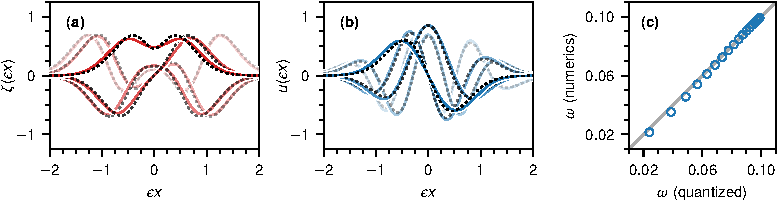
\includegraphics{localization/rod_poschl_sech.pdf}
  \end{center}
  \caption{%
    The first five extensional bound states of a rod with a sech-type curvature profile showing (a) the normal component $\zeta(x)$ and (b) the tangential component $u(x)$.
    Lighter curves in (a) and (b) depict higher-frequency states and the dashed black curves represent the solutions obtained analogously to those in Eq.~\eqref{eq:poschl} after setting $b^{2} \to b^{2} - a^{2}$ and $\epsilon \to \chi\epsilon$.
    (c) Comparison between the bound-state frequencies $\omega$ obtained through quantization, and those from numerics [cf.~Fig.~\ref{fig:rod_wkb}(b)].
  }
  \label{fig:poschl_sech}
\end{figure}

At this juncture, let us remark that Eq.~\eqref{eq:schrodinger} can also be derived by diagonalizing the full wave equation in Eq.~\eqref{eq:rod} using the asymptotic method outlined by Littlejohn and coworkers~\cite{littlejohn1991,littlejohn1991a,weigert1993}, without appealing to any physical arguments.
In this method, the operators of the diagonalized equations in symbol form are the two eigenvalues $\lambda_{\pm}$ of the dispersion matrix $\mathsf{D}^{(0)}$.
To find the extensional bound states, we focus on $\lambda_{+}$, the ray Hamiltonian for extensional waves.
Instead of using $\lambda_{+}$ from Eq.~\eqref{eq:rod_ham}, which involves a radical expression, we use the approximate version $\lambda_{+} \approx k^{2} - m^{2} - \omega^{2}$ [see Eqs.~\eqref{eq:rod_kgm} and \eqref{eq:rod_klm}].
Next, we promote $k \to \hat{k} = -i\partial_{x}$, which ``quantizes'' the ray Hamiltonian $\lambda_{+}$ and we obtain Eq.~\eqref{eq:schrodinger} for an unknown wave function $\phi(x)$.
The full wave field can be recovered from $\phi(x)$ using $(\zeta, u) \sim \hat{\tau}_{+}\phi(x)$, where $\hat{\tau}_{+}$ is a two-component operator obtained by promoting $k \to \hat{k}$ in the symbol form of the polarization vector $\tau_{+}$.
From Eq.~\eqref{eq:rod_tau}, we see that $\tau_{+} \approx [m(x),\, ik]$ so that $\hat{\tau}_{+} \approx [m(x),\, \partial_{x}]$.
We then find $\zeta(x) \sim m(x)\phi(x)$ and $u(x) \sim \partial_{x}\phi(x)$, consistent with our analysis.

\section{Higher-order rod equations}
\label{sec:rod_ho}

A slightly different set of rod equations, with higher-order curvature-dependent terms is sometimes considered instead of the equations that we have been using.
Given the ubiquity of the higher-order equations,%
\footnote{See, e.g., Eq.~(30) of Ref.~\cite{morley1961}, Eq.~(3.5.24) of Ref.~\cite{graff1991}, and Eq.~(3.34) of Ref.~\cite{doyle2021}.}
it is useful to briefly discuss them here and contrast the results to those obtained so far.
The higher-order rod model is derived from the following energy functional:
%
\begin{equation}
  \mathscr{U}[\zeta, u] = \int \dd{t}\,\dd{x}\,\tfrac{1}{2}\left\{\rho\left(\dot{u}^{2} + \dot{\zeta}^{2}\right) - E\left[\partial_{x}u - m(x)\zeta\right]^{2} - B\left[\partial_{x}^{2}\zeta + m(x)\partial_{x}u\right]^{2}\right\},
  \label{eq:rod_ho_energy}
\end{equation}
%
The only difference between Eq.~\eqref{eq:rod_energy} and Eq.~\eqref{eq:rod_ho_energy} is the curvature-dependent term $m(x)\partial_{x}u$ in the bending energy density, with all other physical parameters having the same meaning.
Using the same nondimensionalization as before, we find that Eq.~\eqref{eq:rod_ho_energy} results in the following equations of motion:
%
\begin{equation}
  \partial_{t}^{2}
  \begin{pmatrix}
    \zeta\\
    u
  \end{pmatrix}
  +
  \widehat{\mathsf{H}}
  \begin{pmatrix}
    \zeta\\
    u
  \end{pmatrix}
  = 0,
  \label{eq:rod_ho}
\end{equation}
%
where the matrix operator
%
\begin{equation}
  \widehat{\mathsf{H}} =
  \begin{pmatrix}
  \partial_{x}^{4} + m^{2} & -m\partial_{x}(1 - \partial_{x}^{2}) + 2m'\partial_{x}^{2} + m''\partial_{x}\\
  m\partial_{x}(1 - \partial_{x}^{2}) + m'(1 - \partial_{x}^{2}) & -(1 + m^{2})\partial_{x}^{2} - 2mm'\partial_{x}
  \end{pmatrix}.
\end{equation}
%
To see why Eq.~\eqref{eq:rod} is a good approximation to Eq.~\eqref{eq:rod_ho},
we write down the dispersion matrix by following the usual procedure of expressing the derivatives in terms of the momentum operator and converting operators to symbols, after which we find%
\footnote{Note that unlike the dispersion matrices in Eq.~\eqref{eq:rod_D}, here we also have an $\mathcal{O}(\epsilon^{2})$ correction $\mathsf{D}^{(2)}$, which we ignore in our analysis.}
%
\begin{equation}
  \mathsf{D}^{(0)}
  =
  \begin{pmatrix}
    k^{4} + m^{2} - \omega^{2} & -imk(1 + k^{2})\\
    imk(1 + k^{2}) & (1+m^{2})k^{2} - \omega^{2}
  \end{pmatrix}
  \quad\text{and}\quad
  \mathsf{D}^{(1)}
  =
  \tfrac{1}{2}
  \begin{pmatrix}
    0 & m'(1-k^{2})\\
    m'(1-k^{2}) & 0
  \end{pmatrix}.
\end{equation}
%
Clearly, for small wave numbers ($k \ll 1$) and weak curvatures ($m \ll 1$), we can drop $k^{2}$ and $m^{2}$ in comparison to unity in the entries of $\mathsf{D}^{(0)}$ and $\mathsf{D}^{(1)}$.
Doing so would lead us back to the dispersion matrices in Eq.~\eqref{eq:rod_D}.
%
\begin{figure}
  \begin{center}
    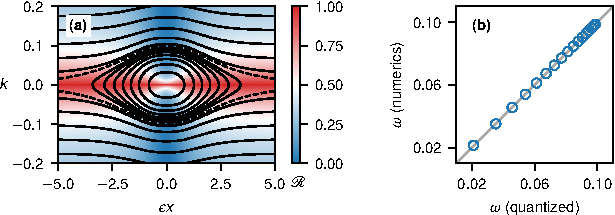
\includegraphics{localization/rod_ho.pdf}
  \end{center}
  \caption{(a) Ray trajectories for extensional waves described by the higher-order rod equations, Eq.~\eqref{eq:rod_ho}, for the sech-type curvature profile $m_{2}(x)$ [cf.~Fig.~\ref{fig:rod_bound}(b)]. (b) Bound-state frequencies obtained from numerics compared to those obtained by quantization.}
  \label{fig:rod_ho}
\end{figure}

The ray Hamiltonian for extensional and flexural waves ($\lambda_{+}$ and $\lambda_{-}$, respectively) are the two eigenvalues of $\mathsf{D}^{(0)}$, given by
%
\begin{equation}
  \lambda_{\pm}(x, k) = \frac{1}{2} \left\{\left[1 + k^2\right] \left[k^2+m^{2}(x)\right]+\sqrt{\left[k^2+1\right]^2 \left[k^2+m^{2}(x)\right]^2-4 \left[k^3-k m^{2}(x)\right]^2}\right\} - \omega^{2}.
\end{equation}
%
A simple analysis, either by plotting the rays or writing down the corresponding Hamilton's equations, reveals that even when higher-order, curvature-dependent corrections are included, flexural waves fail to form bound states, and so we focus on extensional waves instead.
Figure~\ref{fig:rod_ho}(a) shows the ray trajectories for extensional waves described by Eq.~\eqref{eq:rod_ho}.
Clearly, these rays are nearly identical to those seen previously in Fig.~\ref{fig:rod_bound}(b), showing again that the simpler rod equations are an excellent approximation to Eq.~\eqref{eq:rod_ho} in the weak curvature limit.
For the same reason, the frequencies of the extensional bound states obtained through quantization and numerics also tend to agree rather well%
\footnote{Other aspects of quantization, e.g., the lack of the extra phase $\gamma$, location of the turning points, $m^{2}(x^{\star}) = \omega^{2}$, etc., also carry over.}
with our previous results; compare, for example, Fig.~\ref{fig:rod_ho}(b) with Fig.~\ref{fig:rod_wkb}(b).

Let us conclude the discussion on rods by emphasizing that all rod models are approximate to a certain degree.
And although we have limited our analysis to just two models, we expect to see our basic result, i.e., extensional waves forming bound states around points where the absolute curvature has a minimum, in other models as well.
We next turn to wave propagation on curved shells.

\section{Waves on a curved shell}
\label{sec:shell}

One of the simplest shell theories that involve a curvature-mediated coupling between the tangential and normal components of the displacement field is the widely used Donnell--Yu shell model~\cite{donnell1933,yu1955}.
It is simple in the sense that it describes the undulations of a three-dimensional shell solely in terms of the deformation of the shell's two-dimensional midsurface, ignoring higher-order effects and retaining only the lowest-order derivatives.
For an arbitrarily parameterized midsurface, it is easiest to extract the equations of motion from the covariant form of the Donnell--Yu shell equations derived by \citet{pierce1993a}.

\subsection{Equations of motion}

We consider the middle surface of the shell to be a generalized cylinder~\cite{pressley2010} obtained by translating a plane curve $\bm{\sigma}: \mathcal{X} \to \mathbb{R}^{3}$, parameterized by $x \in \mathcal{X} \subset \mathbb{R}$, perpendicular to the plane containing it.
Thus, the shell is defined by $\bm{\Sigma}: \mathcal{X}\times\mathcal{Y} \to \mathbb{R}^{3}$, $\bm{\Sigma}(x, y) = \bm{\sigma}(x) + y{\bm{e}}_{y}$, where $\bm{e}_{y} = \partial_{y}\bm{\Sigma}$ is a constant unit vector perpendicular to the plane containing $\bm{\sigma}(x)$.
Also, $y \in \mathcal{Y}$ is the coordinate along $\bm{e}_{y}$.
For simplicity, and to make comparisons with the rod equations easier, we assume that $x$ is the arclength so that $\bm{e}_{x} = \partial_{x}\bm{\Sigma} = \bm{t}$ is the unit tangent along the curve $\bm{\sigma}$.
Furthermore, we orient $\bm{e}_{y}$ such that surface normal $\bm{e}_{x}\times\bm{e}_{y}$ coincides with the normal $\bm{n}$ to $\bm{\sigma}$.
Then, the only nonvanishing principal curvature of the shell is equal to the curve's signed curvature $m(x)$.
Propagating waves displace the shell from $\bm{\Sigma} \to \bm{\Sigma} + \delta\bm{\Sigma}$.
We write the displacement field $\delta\bm{\Sigma}$ as $\delta\bm{\Sigma} = u\bm{e}_{x} + v\bm{e}_{y} + \zeta\bm{n}$.
Assuming no external forces, the dynamic Donnell--Yu equations are
%
\begin{subequations}
  \begin{align}
    \varrho \frac{\partial^{2}\zeta}{\partial t^{2}} &= -\widetilde{B}\Delta^{2}\zeta - \widetilde{E}m^{2}(x) \zeta + \widetilde{E}m(x)\left(\frac{\partial u}{\partial x} + \eta\frac{\partial v}{\partial y}\right),\\
    \frac{\varrho}{\widetilde{E}} \frac{\partial^{2}u}{\partial t^{2}} &= -\frac{\partial\left[m(x)\zeta\right]}{\partial x} + \frac{\partial^{2}u}{\partial x^2} + \frac{(1-\eta)}{2}\frac{\partial^{2}u}{\partial y^{2}} + \frac{(1+\eta)}{2}\frac{\partial^{2}v}{\partial x \partial y},\\
    \frac{\varrho}{\widetilde{E}} \frac{\partial^{2}v}{\partial t^{2}}&= -\eta m(x)\frac{\partial \zeta}{\partial y} + \frac{(1+\eta)}{2}\frac{\partial^{2}u}{\partial x \partial y} + \frac{(1-\eta)}{2}\frac{\partial^{2}v}{\partial x^{2}} + \frac{\partial^{2}v}{\partial y^2}.
  \end{align}
\end{subequations}
%
Here $\Delta$ is the two-dimensional Laplacian, $\eta$ is the Poisson's ratio, and $\varrho$ is the density per unit area.
Also, the extensional stiffness $\widetilde{E} = Yh/(1-\eta^{2})$ and bending stiffness $\widetilde{B} = Yh^{3}/\left[12(1-\eta^{2})\right]$, with $Y$ being the Young's modulus and $h$ being the thickness of the shell.
On setting the length units to $\sqrt{\widetilde{B}/\widetilde{E}}$ and time units to $\sqrt{\smash[b]{\widetilde{B}\varrho}}/\widetilde{E}$, we arrive at the nondimensional form of these equations, which in matrix form reads
%
\begin{equation}
  \partial^{2}_{t}
  \begin{pmatrix}
    \zeta\\
    u\\
    v
  \end{pmatrix}
  +
  \widehat{\mathsf{H}}
  \begin{pmatrix}
    \zeta\\
    u\\
    v
  \end{pmatrix} = 0,\enspace
\end{equation}
%
where the operator $\widehat{\mathsf{H}}$ is defined by
%
\begin{equation}
  \widehat{\mathsf{H}} =
  \begin{pmatrix}
    \Delta^{2} + m^{2}(x) & -m(x)\partial_x & -\eta m(x) \partial_{y}\\
    m(x)\partial_{x} + m'(x) & -\partial_{x}^{2} - \frac{1}{2}(1-\eta)\partial^{2}_{y} & -\frac{1}{2}(1+\eta)\partial_{x}\partial_{y}\\
    \eta m(x)\partial_{y} & -\frac{1}{2}(1+\eta)\partial_{x}\partial_{y} & -\frac{1}{2}(1-\eta)\partial_{x}^{2} - \partial_{y}^{2}
  \end{pmatrix}.
  \label{eq:shell_wave_eq}
\end{equation}
%
A set of equations analogous to the rod equations [see Eq.~\eqref{eq:rod}] can be obtained by suppressing the $y$ derivatives in the submatrix obtained by deleting the third row and column of the operator $\widehat{\mathsf{H}}$ given above.

Translation invariance of $\widehat{\mathsf{H}}$ along $y$ lets us look for time-harmonic solutions with the common factor $e^{i(ly - \omega t)}$, where $l$ is the transverse wave number in the $y$ direction and $\omega$ is the frequency of oscillation.
This makes the wave field depend only on the coordinate $x$, and makes the transverse wave number $l$ an additional parameter of the operator $\widehat{\mathsf{H}}$.
But the operator $\widehat{\mathsf{H}}$ now has complex coefficients, and the components of its eigenmodes are complex functions.
However, while discussing the numerical results, we use a phase convention such that $\zeta, u$ are real, and $v$ is imaginary.

Similar to what we did for the rod equations, we perform a change of variables $x \to \epsilon^{-1}x$ and recast the spatial derivatives in terms of the momentum operator $\hat{k}$.
Finally, we find the dispersion matrix $\mathsf{D}^{(0)}$ as
%
\begin{equation}
\mathsf{D}^{(0)} =
\begin{pmatrix}
  (k^{2} + l^{2})^{2} + m^{2}(x) - \omega^{2} & -i k m(x) & -i\eta l m(x)\\
  ik m(x) & k^{2} + \frac{1}{2}(1-\eta)l^{2} - \omega^{2} & \frac{1}{2}(1+\eta)kl\\
  i\eta l m(x) & \frac{1}{2}(1 + \eta)kl & \frac{1}{2}(1-\eta)k^{2} + l^{2} - \omega^{2}
\end{pmatrix},\\
\end{equation}
and find its first-order correction $\mathsf{D}^{(1)}$ to be
\begin{equation}
\mathsf{D}^{(1)} =
\frac{1}{2}
\begin{pmatrix}
  0 & m'(x) & 0\\
  m'(x) & 0 & 0\\
  0 & 0 & 0
\end{pmatrix}.
\label{eq:shell_disp_matrices}
\end{equation}
%
For later analysis, it is also useful to note down the determinant%
\footnote{The expression for $\det\mathsf{D}^{(0)}$ in Eq.~\eqref{eq:shell_det} is sometimes referred to as the ``full'' dispersion relation~\cite{sondergaard2002}.  In reality, $\det\mathsf{D}^{(0)}$ is the product of three dispersion relations---a fact that we will later exploit for finding the ray trajectories.}
of $\mathsf{D}^{(0)}$, which is
%
\begin{equation}
  \begin{aligned}
    \det\mathsf{D}^{(0)} &= m^{2}(x)\left\{\left[\omega^{2} - \tfrac{1}{2}(1-\eta)l^{2}\right]\left[\omega^{2}-(1-\eta^{2})l^{2}\right] - \tfrac{1}{2}(1-\eta)k^{2}\omega^{2}\right\} \\
            &\qquad- \left[\omega^{2} - (k^{2} + l^{2})^{2}\right]
            \left[\omega^{2} - \tfrac{1}{2}(1-\eta)(k^{2} + l^{2})\right]
            \left[\omega^{2} - (k^{2} + l^{2})\right].
  \end{aligned}
  \label{eq:shell_det}
\end{equation}
%
Before we continue, it is insightful to examine the dispersion relations for plain waves propagating on singly-curved shells of constant curvature.

\subsection{Shells of constant curvature}

First we analyze the zero curvature limit, i.e., when the shell becomes a flat plate.
In this limit, the wave equation, Eq.~\eqref{eq:shell_wave_eq}, decouples into two equations, the first of which involves only the normal component $\zeta$, and represents flexural waves.
The second equation, representing extensional and shear waves, only involves the tangential components $u$ and $v$.
Shear waves propagate transversely to the in-plane wave vector $k\bm{e}_{x} + l\bm{e}_{y}$, whereas extensional waves are longitudinal to it.
Setting $m = 0$ in Eq.~\eqref{eq:shell_det}, we find the following flat-plate dispersion relations
%
\begin{equation}
  \omega_{0}^{2} = \left(k^{2} + l^{2}\right)^{2},\quad
  \omega_{0}^{2} = \frac{1}{2}\left(1-\eta\right)\left(k^{2} + l^{2}\right),
  \quad\text{and}\quad
  \omega_{0}^{2} = \left(k^{2} + l^{2}\right),
  \label{eq:shell_disp_zero}
\end{equation}
%
which we recognize as the dispersion relations of flexural, shear, and extensional waves, respectively~\cite{fung1965}.
The above dispersion relations for a fixed transverse wave number $l$ are indicated by the dashed black curves in Fig.~\ref{fig:shell_disp}.
Because $l$ is nonzero, there is now a gap in the dispersion curves and a corresponding nonzero cut-on frequency for each of these waves.
%
\begin{figure}
  \begin{center}
    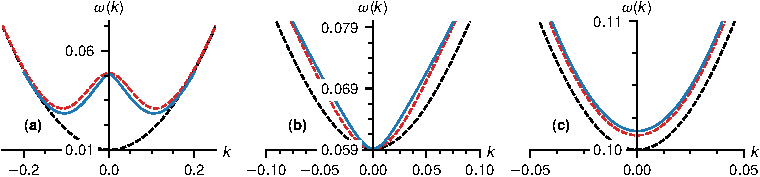
\includegraphics{localization/shell_disp.pdf}
  \end{center}
  \caption{%
    Dispersion curves for plain waves propagating on a cylinder of constant curvature $m = 0.05$ for (a) flexural, (b) shear, and (c) extensional waves.
    In each plot, the solid blue curves represent the actual dispersion curves obtained by finding $\omega$ using Eq.~\eqref{eq:shell_cubic_sol}.
    The dashed red curves represent the approximate dispersion relation in Eq.~\eqref{eq:shell_disp_approx}.
    Also, the dashed black curves indicate the dispersion curves for an uncurved flat plate, i.e., when $m = 0$ [Eq.~\eqref{eq:shell_disp_zero}].
    The transverse wave number $l = 0.1$ and Poisson's ratio $\eta = 0.3$ for all curves.
  }
  \label{fig:shell_disp}
\end{figure}

\subsubsection*{Exact dispersion relations}

For nonzero but constant curvature, plain waves continue to propagate on the shell, which now becomes part of a thin cylinder.
For simplicity, we shall continue to call these waves as being flexural, extensional, or shear in nature.
However, as with the curved rod, we expect some amount of mixing of the tangential and normal displacements due to nonzero curvature.
Also, to find the dispersion relations from Eq.~\eqref{eq:shell_det} we now need to use the general cubic formula~\cite{olver2010}, which results in unwieldy analytical expressions.
More specifically, these relations can be obtained by solving the following cubic in $\omega^{2}$:
%
\begin{equation}
  \omega^{6} - a\omega^{4} - b\omega^{2} - c = 0
\end{equation}
%
where the coefficients
%
\begin{equation}
  \begin{aligned}
    a &= \frac{1}{2}q^{2}\left[(3 - \eta) + 2q^{2}\right],\\
    b &= -\frac{1}{2}q^{4}\left[(3 - \eta)q^{2} + (1 - \eta)\right] - \frac{1}{2}m^{2}(1 - \eta)\left[q^{2} + 2(1 + \eta)l^{2}\right],\\
    c &= \frac{1}{2}(1-\eta)\left[q^{8} + m^{2}l^{4}\left(1 - \eta^{2}\right)\right],
  \end{aligned}
\end{equation}
%
and $q^{2} = k^{2} + l^{2}$ is the magnitude of the wave vector.
The above cubic has the solution
%
\begin{equation}
  \omega^{2} =
  \begin{dcases}
    \frac{1}{3}a + \frac{2^{1/3}\left(a^{2} + 3b\right)}{3d} + \frac{d}{3\times2^{1/3}} & \text{(extensional)},\\
    \frac{1}{3}a - \frac{\left(1 - i\sqrt{3}\right)\left(a^{2} + 3b\right)}{3\times2^{2/3}d} - \frac{\left(1 + i\sqrt{3}\right)d}{6\times2^{1/3}} & \text{(shear)},\\
    \frac{1}{3}a - \frac{\left(1 + i\sqrt{3}\right)\left(a^{2} + 3b\right)}{3\times2^{2/3}d} - \frac{\left(1 - i\sqrt{3}\right)d}{6\times2^{1/3}} & \text{(flexural)}.\\
  \end{dcases}
  \label{eq:shell_cubic_sol}
\end{equation}
%
where
%
\begin{equation}
  d = \left(2 a^3+9 a b+27 c+3 \sqrt{3}\sqrt{4 a^3 c-a^2 b^2+18 a b c-4 b^3+27 c^2}\right)^{1/3}.
\end{equation}
%
It is not directly obvious how the roots in Eq.~\eqref{eq:shell_cubic_sol} can be associated with a specific wave polarization.
To do so, we have to take the limit $m \to 0$ numerically and find which of the roots reduce to the flat-plate results in Eq.~\eqref{eq:shell_disp_zero}.

As an example, using Eq.~\eqref{eq:shell_cubic_sol}, we find the dispersion curves at a curvature value of $m = 0.05$, which are indicated by the solid lines in Fig.~\ref{fig:shell_disp}.
We make two observations on comparing these curves with the dispersion curves for a flat plate:
(i) the gap in the dispersion curves for flexural and extensional waves [Figs.~\ref{fig:shell_disp}(a) and~\ref{fig:shell_disp}(c)] have increased, and the flexural dispersion curve now has a double-well appearance;
(ii) although the dispersion curve for shear waves has changed in appearance [Fig.~\ref{fig:shell_disp}(b)], the gap remains the same and the cut-on frequency remains unchanged.
The cut-on frequencies at nonzero $m$ can be computed from Eq.~\eqref{eq:shell_det} after setting $k = 0$, and we find three roots
%
\begin{equation}
  \omega^{2}_{\text{cut-on}} =
    \frac{1}{2}\left(l^{2} + l^{4} + m^{2} \pm \sqrt{\left(l^{2} - l^{4} - m^{2}\right)^{2} + 4\eta^{2}l^{2}m^{2}}\right)
    \quad\text{and}\quad
    \frac{1}{2}(1-\eta)l^{2}.
    \label{eq:shell_cuton}
\end{equation}
%
Our intuition and a series expansion in $m$ suggests that the lowest of the first two roots must be associated with flexural waves and the highest root must be associated with extensional waves.
The third root, which is independent of the curvature $m$, must then correspond to the cut-on frequency for shear waves.
As we shall see, this association is only correct at very low curvatures.

\subsubsection*{Approximate dispersion relations}

Although the exact dispersion relations for nonzero curvature are unwieldy, we can find an approximate expression for the dispersion relations in the very weak curvature limit.
To this end, we write the roots $\omega^{2}$ as a regular perturbation series~\cite{bender1978} in even powers of $m$, i.e.,
%
\begin{equation}
  \omega^{2}(k, l) = \omega^{2}_{0}(k, l) + \sum_{n = 1}^{\infty} m^{2n}Q_{n}(k, l),
  \label{eq:shell_perturb}
\end{equation}
%
where $\omega_{0}$ is one of the three roots in Eq.~\eqref{eq:shell_disp_zero} and $Q_{n}(k, l)$ are coefficients to the correction terms that we have to determine.%
\footnote{Note that it is a futile task to expand the roots in Eq.~\eqref{eq:shell_cubic_sol} in powers of $m$ to find the approximate dispersion relationships.}
Since the curvature is assumed to be very weak, the dispersion relations obtained this way can be associated with a wave type based on the choice we make for $\omega_{0}$.
Putting Eq.~\eqref{eq:shell_perturb} in Eq.~\eqref{eq:shell_det}, and dropping powers of $k$ and $l$ in comparison to unity, we find
%
\begin{equation}
  \omega^{2} =
  \begin{dcases}
    \left(k^{2} + l^{2}\right)^{2} + \left(1 - \eta^{2}\right)m^{2}\frac{l^{4}}{\left(k^{2} + l^{2}\right)^{2}} + \mathcal{O}(m^{4}) & \text{(flexural)}, \\
    \frac{1}{2}\left(1-\eta\right)\left(k^{2} + l^{2}\right) + 2\left(1 - \eta\right)m^{2}\frac{k^{2}l^{2}}{\left(k^{2} + l^{2}\right)^{2}} + \mathcal{O}(m^{4}) & \text{(shear)},\\
    (k^{2} + l^{2}) + m^{2}\frac{\left(k^{2} + \eta l^{2}\right)^{2}}{\left(k^{2} + l^{2}\right)^{2}} + \mathcal{O}(m^{4}) & \text{(extensional)}.
  \end{dcases}
  \label{eq:shell_disp_approx}
\end{equation}
%
The above approximate dispersion relations are identical to those found in the literature and derived using alternative approaches~\cite{germogenova1973,pierce1993,norris1994,rebinsky1996}.
Also, in their analytical characterization of bound waves in a musical saw, \citet{shankar2022} works exclusively with the above approximate dispersion relation for flexural waves, which has also been observed experimentally~\cite{williams1990}.
In Fig.~\ref{fig:shell_disp}, the approximate dispersion relations for $m = 0.05$ are indicated by the red dashed curves, from which we can see that Eq.~\eqref{eq:shell_disp_approx} captures the true dispersion relations to a reasonably good accuracy.

Equation~\eqref{eq:shell_disp_approx} must break down beyond a certain value of the curvature.
Indeed, we only expect it to capture the true dispersion when the $\mathcal{O}(m^{2})$ correction term in Eq.~\eqref{eq:shell_perturb} is smaller than $\omega_{0}^{2}$, and more conservatively, only when $m \ll k^{2} + l^{2}$.
We would expect the dispersion relation to deviate significantly from Eq.~\eqref{eq:shell_disp_approx} as $m$ increases.
In fact, for small $k$ and $l$, Eq.~\eqref{eq:shell_disp_approx} completely breaks down at a curvature at which the cut-on frequency for flexural and extensional waves become equal.
For nonzero $l$, from Eq.~\eqref{eq:shell_cuton}, we see that this happens at a curvature value
%
\begin{equation}
  m_{\ddag}^{2} = \frac{(1 + \eta)l^{2}\left[\frac{1}{2}(1 - \eta) - l^{2}\right]}{\left(1 + 2\eta\right)\left(1 - \eta\right)}
  = \frac{1}{2}\left(\frac{1+\eta}{1 + 2\eta}\right)l^{2} + \mathcal{O}(l^{4}).
  \label{eq:shell_mdag}
\end{equation}
%
We graphically demonstrate this in Fig.~\ref{fig:shell_gap}, from which we can see that the expressions for the cut-on frequencies for shear and flexural waves get interchanged at large $m$.
Hence, for $m > m_{\ddag}$, the lowest of the first two cut-on frequencies in Eq.~\eqref{eq:shell_cuton}, should be associated with shear waves, whose dispersion curves would now have a curvature-dependent gap.
The cut-on frequency for flexural waves, however, would now be equal to $\frac{1}{2}(1-\eta)l^{2}$.
We remark that this switching of the cut-on frequencies does not happen if $l^{2} > \frac{1}{2}(1-\eta)$ as Eq.~\eqref{eq:shell_mdag} fails to have a real root.
Also, as the cut-on frequencies of flexural and shear waves are equal for $m = m_{\ddag}$, in principle, mode conversion can occur close to the entire $k$ axis on the phase plane.
Despite such a possibility, we did not observe any discernible effects of mode conversion in our numerical experiments, and we shall it ignore in our analysis.
%
\begin{figure}
  \begin{center}
    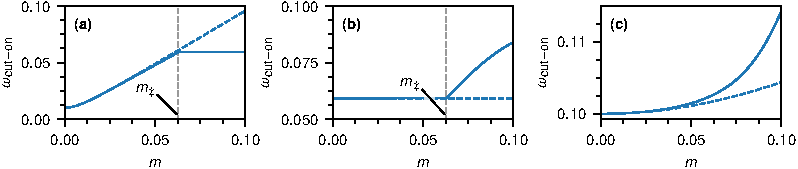
\includegraphics{localization/shell_gap.pdf}
  \end{center}
  \caption{%
    Cut-on frequencies for a singly-curved shell as a function of the curvature $m$ for (a) flexural, (b) shear, and (c) extensional waves.
    The blue dashed curves represent the cut-on frequency predicted by Eq.~\eqref{eq:shell_disp_approx}, which holds only when $m$ is small.
    The solid curves represent the actual cut-on frequency obtained by finding $\omega$ from Eq.~\eqref{eq:shell_det} using the general cubic formula, and taking the limit $k \to 0$ numerically.
    The transverse wave number $l = 0.1$ and Poisson's ratio $\eta = 0.3$ in all plots.
  }
  \label{fig:shell_gap}
\end{figure}

\subsection{Shells with varying curvature}

We shall now consider singly-curved shells with varying curvature profiles.
Given the complexity of the general dispersion relations and the myriad of subtleties, we shall, however, perform a less exhaustive analysis compared to what we did for the rod.
We shall only look at a limited number of examples, and to simplify matters, we set the transverse wave number $l = 0.1$ and Poisson's ratio $\eta = 0.3$ (corresponding to that of steel) throughout.
As for the rod, we will consider both tanh-type and sech-type curvature profiles, but we assume that the largest absolute curvature $b > m_{\ddag}$.
This would let us examine the problem beyond the range of validity of the approximate dispersion relation in Eq.~\eqref{eq:shell_disp_approx}.
For the sech-type curvature profile, we additionally assume that the smallest curvature $a < m_{\ddag}$.
With $l = 0.1$ and $\eta = 0.3$, we have $m_{\ddag} \approx 0.06$, and these assumptions are satisfied by the choices $a = 0.01$ and $b = 0.1$ that we made for the rod, and we use them for the shell as well.

From our earlier analysis, we saw that the spectral gap in the dispersion relation for all three wave polarizations grows with increasing curvature.
Now, consider a wave traveling from a region of low curvature to one of high curvature.
As the wave moves, at some point, the frequency of the wave would fall below the local cut-on frequency of waves, where it gets reflected back.
Intuitively, we therefore expect bound states to occur for all three wave polarizations.
%
\begin{figure}
  \begin{center}
    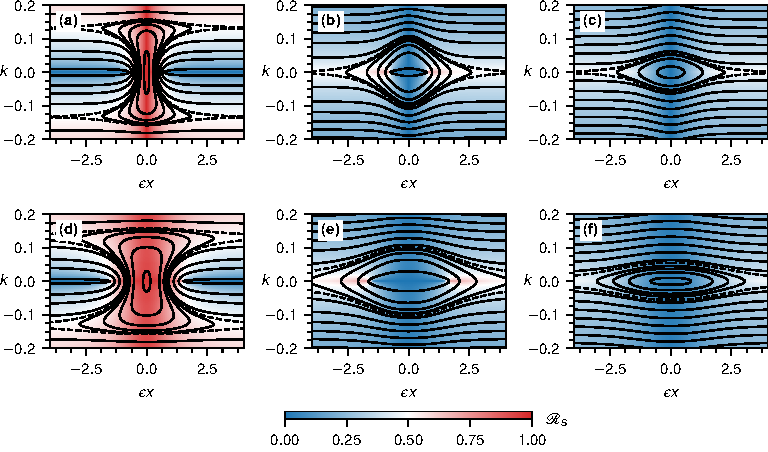
\includegraphics{localization/shell_rays.pdf}
  \end{center}
  \caption{%
    Rays trajectories for a curved shell with a tanh-type curvature profile (top panels) and a sech-type curvature profile (bottom panels) showcasing (a), (d) flexural waves, (b), (e) shear waves, and (c), (f) extensional waves.
    In all figures the closed curves represent rays associated with quantized bound states and the dashed black curves represent the highest frequency for which there is a bound state.
    The phase portraits have also been color coded with the ratio $\mathscr{R}_{s}$ defined in Eq.~\eqref{eq:shell_ratio}.
  }
  \label{fig:shell_rays}
\end{figure}

For ray analysis, we usually directly work with the eigenvalues of the dispersion matrix $\mathsf{D}^{(0)}$.
This proves to be difficult for the shell as the expressions for the eigenvalues are unwieldy.
In the absence of mode conversion, however, only one eigenvalue, say $\lambda$, will vanish at a given phase-space point $(x, k)$, causing the determinant $\det\mathsf{D}^{(0)}$ to vanish as well.
Hence, the rays determined by $\lambda(x, k; \omega) = 0$ and $\det\mathsf{D}^{(0)} = 0$ are identical, allowing us to use $\det\mathsf{D}^{(0)}$ as the ray Hamiltonian.%
\footnote{Let us remark that the ray trajectories can also be obtained by treating $\omega^{2}$ in Eq.~\eqref{eq:shell_cubic_sol} as the ray Hamiltonian.  However, given the general awkwardness of the expressions, it is better to work with $\det\mathsf{D}^{(0)}$ instead.}
Using $\det\mathsf{D}^{(0)}$ instead of $\lambda$ would amount to a trivial reparameterization of Hamilton's equations~\cite{tracy2014}.
Judicious choices of the initial conditions, i.e., the coordinates $(x, k)$ and frequency $\omega$, obtained from the local dispersion curves at a given $(x, k)$, would determine the type of wave the ray represents.
When analyzing a given wave type, it is also useful to compute an amplitude ratio, analogous to the one we used for the curved rod, and defined by
%
\begin{equation}
  \mathscr{R}_{s} = \frac{\abs{\zeta}}{\abs{\zeta} + \abs{u} + \abs{v}} \sim \frac{\abs{\tau_{1}}}{\abs{\tau_{1}} + \abs{\tau_{2}} + \abs{\tau_{3}}}.
  \label{eq:shell_ratio}
\end{equation}
%
Above, we have also made use of the fact that the wave field is asymptotic to the polarization vector $\tau$ to write $\mathscr{R}_{s}$ in terms of the components of $\tau$.
With the above definition, flexural waves in a flat plate have $\mathscr{R}_{s} = 1$, whereas both shear and extensional waves have $\mathscr{R}_{s} = 0$.
In a curved shell, because we expect both the normal and tangential components of the wave field to be significant, $\mathscr{R}_{s}$ for the three wave polarizations would deviate from their flat-plate counterparts.
For all three wave types, a significant amount of normal and tangential contribution to the displacement field is indicated by values of $\mathscr{R}_{s}$ in the range $1/3 < \mathscr{R}_{s} < 1/2$.
We discuss flexural waves first.

\subsubsection*{Flexural waves}
\label{sec:shell_flexural}

Our intuitive expectation of flexural bound states is confirmed by the actual ray trajectories for flexural waves showcased in Figs.~\ref{fig:shell_rays}(a) and~\ref{fig:shell_rays}(d).
For frequencies slightly above the cut-on frequency at $x = 0$, the rays appear in the form of closed, vertically-elongated orbits that remain confined to a region where the curvature is very small.
At larger frequencies, the rays begin to enter regions of higher curvature, and orbits change from being elliptical to highly eccentric, ``peanut''-shaped curves.
For these orbits, we have a total of six caustics where $\dot{x} = 0$.
[Compare Figs.~\ref{fig:shell_rays}(a) and~\ref{fig:shell_rays}(d) with Fig.~\ref{fig:caustic}(b).]
Two of these caustics, which are on the $x$ axis, are the usual classical turning points where $k = 0$.
At the other four caustics $k \neq 0$, and they arise due to the two double-well minima in the (local) dispersion curves where $\dd{\omega}/\dd{k} = 0$.

For the peanut-shaped orbits, bound states do not occur beyond a frequency where the four caustics with $k \neq 0$ get pushed to $x = \pm \infty$.
Since the absolute curvature $\abs{m(\pm \infty)} = b$ for both curvature profiles, the largest frequency for which we see a bound state---represented by the dashed rays in Figs.~\ref{fig:shell_rays}(a) and~\ref{fig:shell_rays}(d)---must be the frequency of the double-well minimum in the dispersion curves for $m = b$.
For small enough $b$, using Eq.~\eqref{eq:shell_disp_approx}, we find this minimum to be $\omega^{2} \approx 2\sqrt{l^{4}b^{2}(1-\eta^{2})}$.
This expression, however, turns out to overestimate the actual minimum for larger $b$, and we must find it numerically.
Also, this minimum exists only when $b \gtrsim l^{2}/\sqrt{1-\eta^{2}}$.
For smaller $b$, rays of the bound states remain elliptical in nature, with the classical turning points being the only caustics.

An example profile of a low-frequency flexural bound state is shown in Fig.~\ref{fig:shell_modes_tanh}(a).
This state has negligible tangential components $u$ and $v$, and remains confined to a region of similar extent as the classical turning points.
At higher frequencies, flexural bound states grow beyond the classical turning points and enter regions of higher curvature.
Here curvature effects become more prominent, and the states tend to have both tangential and normal components as seen from Fig.~\ref{fig:shell_modes_tanh}(b), and the color coding of the phase portraits.
They, however, remain confined to a region of similar extent as the four caustics with $\dot{x} = 0$.
%
\begin{figure}
  \begin{center}
    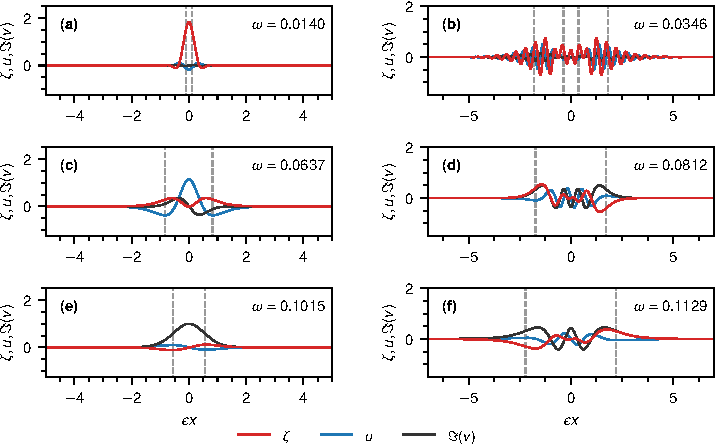
\includegraphics{localization/shell_modes_tanh.pdf}
  \end{center}
  \caption{
  Numerical eigenmodes of a curved shell with a tanh-type curvature profile showing (a),(b) flexural, (c),(d) shear, and (e),(f) extensional bound states.
  In our phase convention, $\zeta$ and $u$ are always real, whereas $v$ is always complex, which is why we only show its imaginary component $\Im(v)$.
  Left panels depict low-frequency bound states, whereas the ones on the right panels have a higher frequency.
  The dashed vertical lines indicate the locations of the caustics.
}
  \label{fig:shell_modes_tanh}
\end{figure}

\subsubsection*{Shear waves}

From the phase portraits in Fig.~\ref{fig:shell_rays}(b) and~\ref{fig:shell_rays}(e), we see that shear waves also form bound rays confined between two classical turning points.
As the frequency of the orbits increase, the turning points move to $x = \pm \infty$, where the absolute curvature for both curvature types is $b$.
Thus, the largest frequency for which we observe shear bound states is the shear-wave cut-on frequency for a cylindrical shell of curvature equal to $b$, obtained by setting $m = b$ in the second root of Eq.~\eqref{eq:shell_cuton}.
Beyond this frequency, shear waves form unbound states.
The rays of shear bound states are elongated along the $x$ direction as the spectral gap in the local dispersion curve does not begin increasing until $m(x) > m_{\ddag}$.
For the same reason, shear waves do not get localized if $b < m_{\ddag}$.
It is then natural to wonder if the localization of shear waves seen in the phase portraits is an artifact of having chosen a relatively large value of $b = 0.1$.
But from Eq.~\eqref{eq:shell_mdag} we see that $m_{\ddag}$ can be made arbitrarily small by adjusting the value of transverse wave number $l$, so that even for small $b$ we would expect shear bound states.

Example profiles of two shear bound states are shown in Figs.~\ref{fig:shell_modes_tanh}(c) and~\ref{fig:shell_modes_tanh}(d).
The first one has a frequency that is only slightly above the shear-wave cut-on frequency and hence its local wave number $k$ is small.
Therefore, its (local) wave vector is predominantly in the $y$ direction [see Fig.~\ref{fig:waves}(b)].
Furthermore, as expected from the transverse nature of shear waves, the dominant tangential component is $u$, which is the displacement along $x$.
The second shear bound state shown in Fig.~\ref{fig:shell_modes_tanh}(f) has a higher frequency, causing it to spread to regions of higher curvature, where curvature effects become more prominent.
This can also be inferred from the color coding of Figs.~\ref{fig:shell_rays}(b) and~\ref{fig:shell_rays}(e), which shows that shear bound states develop a significant normal component at higher frequencies.

\subsubsection*{Extensional waves}

Color-coded phase portraits of extensional waves indicating bound states are shown in Figs.~\ref{fig:shell_rays}(c) and~\ref{fig:shell_rays}(f).
The caustics for these bound states are the usual classical turning points with $k=0$.
For higher-frequency bound states, these points move to $\pm \infty$, where the absolute curvature is $b$.
Hence, the largest frequency for which we observe extensional bound states must be the cut-on frequency for extensional waves in a shell having a curvature equal to $b$, obtained by putting $m = b$ in the first root in Eq.~\eqref{eq:shell_cuton}.

Example profiles of two extensional bound states are shown in Figs.~\ref{fig:shell_modes_tanh}(e) and~\ref{fig:shell_modes_tanh}(f).
Low-frequency extensional bound states, such as the one in Fig.~\ref{fig:shell_modes_tanh}(e), are expected to displace the shell predominantly in the $y$ direction as seen from the comparatively large values of the tangential component $v$.
The bound state in Fig.~\ref{fig:shell_modes_tanh}(f) has a slightly higher frequency, causing it to spread to regions of higher curvature, where it develops a significant normal component, which we also infer from the color coding of Figs.~\ref{fig:shell_rays}(c) and~\ref{fig:shell_rays}(f).

\subsubsection*{Bound states and quantization}

To find the bound-state frequencies, we first set $k=0$ in Eq.~\eqref{eq:shell_det} and rearrange terms to find that that classical turning points $x^{\star}$ are given by the solutions to the implicit equation
%
\begin{equation}
  m^{2}(x^{\star}) = \left[\frac{\omega^{2} - l^{2}}{\omega^{2} - \left(1-\eta^{2}\right)l^{2}}\right]\left(\omega^{2}-l^{4}\right).
  \label{eq:shell_caustic}
\end{equation}
%
Depending on the value of $\omega$, the turning points found using the above equation could correspond to turning points on the bound rays of all three waves.
We use the same quantization procedure as for the rod to determine the bound-state frequencies (Appendix~\ref{app:numerical}).
Furthermore, the extra phases $\gamma_{\text{G}}$ and $\gamma_{\text{NG}}$ in the quantization condition in Eq.~\eqref{eq:quantization} vanish for the shell equations as well (Appendix~\ref{app:additional_phase}).
The Keller--Maslov index continues to be $\alpha = 2$ for all orbits---including the peanut-shaped orbits with six caustics---as they can be smoothly deformed into a circle centered around the origin~\cite{percival1977}.
From Fig.~\ref{fig:shell_wkb}, we see that the bound-state frequencies obtained through quantization agree rather well with the numerical values for both curvature profiles.
% Also, from Fig.~\ref{fig:shell_rays} we see that the sech-type orbits generally enclose a larger area compared to the tanh-type orbits.
% Hence, it is not surprising that a sech-type shell possesses more bound states for all three wave polarizations.
%
\begin{figure}
  \begin{center}
    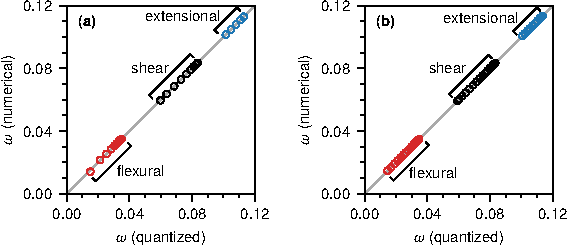
\includegraphics{localization/shell_wkb.pdf}
  \end{center}
  \caption{
    Bound-state frequencies of a curved shell obtained from numerics compared to that obtained through quantization for (a)
    tanh-type curvature profile $m_{1}(x)$ and (b) sech-type curvature profile $m_{2}(x)$.
    For both plots, the gray guide line in the background represents $\omega$ (quantized) = $\omega$ (numerical).
  }
  \label{fig:shell_wkb}
\end{figure}

Although waves of all three types form bound states, from our preceding analyses and Fig.~\ref{fig:shell_wkb}, we see that flexural bound states appear first, followed by shear and extensional bound states.
Thus, in very long shells, shear waves form bound states that lie in a quasi-continuum of flexural waves spread across the shell.
Likewise, extensional bound states would lie in a quasi-continuum of unbound flexural and shear waves.
Similar to the curved rod, the bound states of the curved shell are also of definite parity when the curvature profile $m(x)$ is odd or even.
More specifically, when $m(x)$ is even, the components $\zeta(x)$ and $v(x)$ have the same parity, with $u(x)$ having the opposite parity.
For odd $m(x)$, however, $\zeta(x)$ and $u(x)$ have the same parity, with $v(x)$ having the opposite parity, as can be seen from the example bound states in Fig.~\ref{fig:shell_modes_tanh}.

% Parity analysis
% ---------------
%
% Let also remark that the bound states of all three wave polarizations are also of definite parity when the curvature $m(x)$ is odd or even.
% From Eq.~\eqref{eq:shell_wave_eq}, we can verify that for an odd $m(x)$, if $\psi(x) = \left[\zeta(x), u(x), v(x)\right]$ is an eigenmode, then $\psi(x) = \left[\zeta(-x), u(-x), -v(-x)\right]$ is an eigenmode as well.
% Assuming nondegeneracy, this implies that the real and complex components of $\zeta(x)$ and $u(x)$ have the same parity, i.e., they are both odd or both even.
% The components of $v(x)$, however, would have the opposite parity.
% For the odd tanh-type curvature profile, we see this in Figs.~\ref{fig:shell_modes_tanh}(a)--(c), where $\zeta(x)$ and $u(x)$ are even, and $\Im\left[v(x)\right]$ is odd.
% Similarly, in Figs.~\ref{fig:shell_modes_tanh}(d)--(f), we observe that $v(x)$ is even, and $\zeta(x)$ and $u(x)$ are odd.
% A similar analysis reveals that for an even $m(x)$, the components of $\zeta(x)$ and $v(x)$ have the same parity, with the components of $u(x)$ having the opposite parity.

\section{Shells with sharp bends}

Flexural bound states have also been predicted to exist in curved shells around points of maximal curvature~\cite{mohammed2021}.
To illustrate this, we consider the curvature profile%
\footnote{The authors of Refs.~\cite{sondergaard2002,mohammed2021} use a much more complicated curvature profile in their analysis.  However, for our purposes, $m_{3}(x)$ has the basic features of the profiles that these authors consider.}
$m_{3}(x) = b\sech(\epsilon x)$.
For the parameter values $b = 0.1$ and $\epsilon = 0.01$, Fig.~\ref{fig:shell_m3_profile} shows the function $m_{3}(x)$ and the shape of a curve with this curvature profile.
Clearly, the curve intersects itself at multiple points, and hence $m_{3}(x)$ can only be the curvature profile of a physically unrealizable ``phantom'' shell that allows self intersections.
Although self intersections can be avoided by choosing a smaller value for $b$ (or a larger value for $\epsilon$), doing so would lead to the formation of very few or barely discernible bound states.
For this reason, we will continue to work with the choice $b=0.1$ so that the bound states appear more conspicuous, enabling us to better test our conclusions from a semiclassical analysis.
%
\begin{figure}
  \begin{center}
    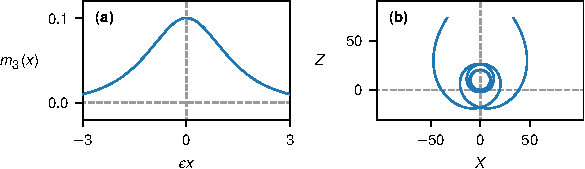
\includegraphics{localization/m3_sech_profile.pdf}
  \end{center}
  \caption{%
    (a) Curvature profile $m_{3}(x) = b\sech{\epsilon x}$ and (b) a curve with this curvature profile in Cartesian space with coordinates $X$ and $Z$.
    As the curve has multiple self intersections, only a physically unrealistic ``phantom'' shell can have this curvature profile.
    The parameters $b = 0.1$ and $\epsilon = 0.01$.
  }
  \label{fig:shell_m3_profile}
\end{figure}

Ray trajectories of all three wave types for the curvature profile $m_{3}(x)$ are shown in Fig.~\ref{fig:shell_m3_rays}.
As we see from this figure, only flexural waves form bound states.
For this reason, we forgo a more detailed analysis of shear and extensional waves, and concentrate on flexural waves alone.
In the phase portrait of Fig.~\ref{fig:shell_m3_rays}(a), we see that in addition to the nonlinear center at the origin, there are two saddle points on the $k$ axis.
The saddle points arise because of the double-well minimum in the flexural dispersion curves where $\dd{\omega}/\dd{k} = 0$.
A more detailed analysis of the phase portraits and bound states of flexural waves reveals the following:
%
\begin{enumerate}
  \item
    The existence of bound states around regions of high curvature cannot simply be explained by considering the gap and/or cut-on frequency in the dispersion curves---after all, as we move away from regions of high curvature to regions of low curvature, this gap decreases.
    In reality, these bound states arise due to the double-well nature of the flexural dispersion curves at nonzero curvature.
    Indeed, if $l = 0$ or $b \lesssim l^{2}/\sqrt{\smash[b]{1-\eta^{2}}}$, the dispersion curves fails to have a double-well nature and bound states do not exist.%
    \footnote{This should be contrasted with flexural bound states around points of minimal curvature, which continue to exist even for $b \lesssim l^{2}/\sqrt{\smash[b]{1-\eta^{2}}}$; see the discussion on p.~\pageref{sec:shell_flexural}.}
  \item Smaller orbits in the phase portraits represent bound states of \emph{higher} frequency.
    Hence, higher-frequency bound states are represented by a smaller quantum number $n$.
    The smallest bound orbit has a frequency slightly above the cut-on frequency of flexural waves at curvature $m = b$.
    For $b > m_{\ddag}$, as the frequency of the orbit approaches the cut-on frequency, the whole orbit flattens to a small line segment on the $x$ axis; for $b < m_{\ddag}$, the orbit shrinks to the origin. [See Eq.~\eqref{eq:shell_mdag} for the definition of $m_{\ddag}$.]
  \item As the frequency of the bound orbits gets smaller, they increase in size, but remain confined between the two heteroclinic orbits [shown as dashed curves in Fig.~\ref{fig:shell_m3_rays}(a)] connecting the saddle points on the $k$ axis.
    The heteroclinic orbits have a frequency equal to the double-well minimum in the dispersion curves, which puts a limit on the \emph{lowest} frequency for which we expect a bound mode.
  \item Incoming and outgoing rays close to the saddle point are nearly tangent to each other, leading to the formation of a tunneling region around the saddle point.%
    \footnote{\citet{mohammed2021} presents a detailed analysis of this tunneling phenomenon.}
    In this region, waves represented by one ray can transfer their energy to waves represented by the other ray~\cite{tracy2014}, which causes the lower-frequency bound states to ``leak out'' as shown in Fig.~\ref{fig:shell_m3_results}(a).
    This, however, does not seem to have a considerable effect on the quantization results, and we recover the frequencies of the observed bound modes accurately [see Fig.~\ref{fig:shell_m3_results}(c)].
  \item Finally, bound states at higher frequencies, such as the one in Fig.~\ref{fig:shell_m3_results}(b), tend to have fewer nodes and appear to be more spatially confined.%
    \footnote{This is in contrast to all the bound states, including those on the curved rod, that we have described so far.}
    They also have more significant tangential contribution as evident from the color coding of Fig.~\ref{fig:shell_m3_rays}(a).
\end{enumerate}
%
\begin{figure}
  \begin{center}
    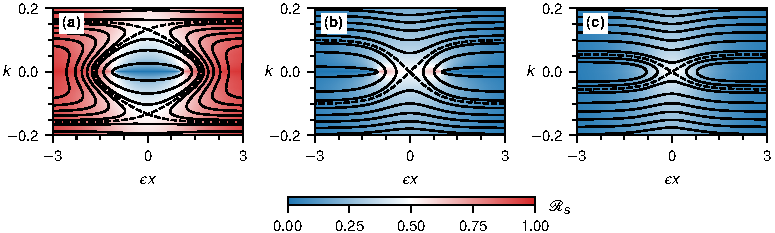
\includegraphics{localization/shell_rays_altsech.pdf}
  \end{center}
  \caption{%
    Rays trajectories for a curved shell with the curvature profile $m_{3}(x)$ showing (a) flexural waves, (b) shear waves, and (c) extensional waves.
    Only flexural waves form bound states.
    The phase portraits are color coded with the ratio $\mathscr{R}_{s}$ defined in Eq.~\eqref{eq:shell_ratio}.
  }
  \label{fig:shell_m3_rays}
\end{figure}

In summary, flexural bound states in a shell can also develop around points of maximal curvature.
Let us again remark, however, that for the parameter choices $b = 0.1$ and $\epsilon = 0.01$, the curvature profile $m_{3}(x)$ is a physical unrealizable one.
On the other hand, numerical experiments with more realistic shells (with small $b$ and/or large $\epsilon$) revealed very few or practically nonexistent bound states---something that we expect to happen in real experiments as well.

\begin{figure}
  \begin{center}
    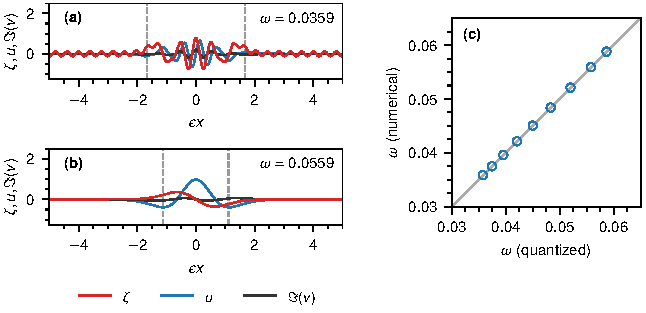
\includegraphics{localization/shell_altsech_results.pdf}
  \end{center}
  \caption{%
    (a), (b) Example flexural bound states for a shell with curvature profile $m_{3}(x)$; the grey vertical lines indicate the locations of the classical turning points.
    Tunneling effects around the saddle points cause the lower-frequency modes, such as the one in~(a), to leak out.
    (c) Comparison between the quantization results and numerics; the grey guideline in the background represents $\omega~\text{(quantized)} = \omega~\text{(numerical)}$.
  }
  \label{fig:shell_m3_results}
\end{figure}

\section{Concluding remarks}
\label{sec:conclusion}

In this chapter we have considered the localization of waves in thin elastic structures induced by variations in the structure's curvature profile.
For both the example structures we considered, bound states develop around points where the structure's absolute curvature has a minimum.
In case of the shell, flexural, shear, and extensional waves form bound states.
Additionally, flexural bound states can also develop around points of a shell where the absolute curvature has a maximum.
In contrast to shells, bound states in a curved rod (which are always extensional in nature) only exist around points where the absolute curvature has a minimum.
These findings set the stage for the design of simple devices capable of inducing wave localization without relying on metamaterials with nontrivial microstructure.

Semiclassical approximation presents challenges of its own when used to study multicomponent waves, particularly due to the presence of nontrivial phases in the quantization rule.
The rod and shell equations we use in this paper, however, have properties that cause these phases to vanish.
Nevertheless, topologically protected waves in continuous media can arise when this phase is nonzero, especially when time-reversal symmetry is broken~\cite{venaille2023}.
For this reason, it is worthwhile to explore the use of semiclassical methods in problems with broken time-reversal symmetry such as those in rotating elastic media~\cite{marijanovic2022}, fluids with odd viscosity~\cite{souslov2019}, and magnetoelastic waves~\cite{banos1956}, where one would generically expect this phase to be nonzero.

\begin{subappendices}

\section{Additional phases}
\label{app:additional_phase}

In this appendix we will look at situations where the extra phase $\gamma$ that appears in the quantization condition in Eq.~\eqref{eq:quantization} vanishes.
As we described in the main text, $\gamma = \gamma_{\text{G}} + \gamma_{\text{NG}}$, where $\gamma_{\text{G}}$ is the term that gives rise to a nonzero geometric phase and $\gamma_{\text{NG}}$ is the other (non-geometric) term.
First, we shall analyze general $N$-component wave equations with an $N\times N$ dispersion matrix $\mathsf{D}^{(0)}$.

\subsection{General wave equations}
\label{app:genwave}

Consider a general $N$-component polarization vector $\tau$ of the dispersion matrix $\mathsf{D}^{(0)}$, given by
%
\begin{equation}
  \tau =
  \left[
    r_{1}(x, k) e^{i{\varphi}_{1}(x,k)},\;
    r_{2}(x, k) e^{i{\varphi}_{2}(x, k)},\;
    \ldots,\;
    r_{N}(x, k) e^{i{\varphi}_{N}(x, k)}
  \right].
  \label{eq:tau}
\end{equation}
%
Above, we have expressed the $j$th component $\tau_{j}$ in terms of a real amplitude $r_{j}(x, k)$ and a phase $\varphi_{j}(x, k)$, both of which are functions of the phase-space coordinates $(x,k)$.
Since $\tau$ is normalized, we have $\Abs{\tau}^{2} = \sum_{j=1}^{n} r_{j}^{2}(x, k) = 1$ for all $(x, k)$.
Putting Eq.~\eqref{eq:tau} in Eq.~\eqref{eq:extra_phases}, we see that the rate of change of the first (geometric) phase $\gamma_{\text{G}}$ is
%
\begin{equation}
  \begin{aligned}
    \dot{\gamma}_{\text{G}} = i\tau^{*}_{j}\left\{\tau_{j}, \lambda\right\}
                  &= ir_{j}\left\{r_{j}, \lambda\right\} - r_{j}^{2}\left\{\varphi_{j}, \lambda\right\}\\
                 &= \frac{i}{2}\left\{\Abs{\tau}^{2}, \lambda\right\} - r_{j}^{2}\left\{\varphi_{j}, \lambda\right\}\\
                 &= -r_{j}^{2}\left\{\varphi_{j}, \lambda\right\}.
  \end{aligned}
\end{equation}
%
In the last step above, we have made use of the fact that $\Abs{\tau} = 1$ always so that $\left\{\Abs{\tau}^{2}, \lambda\right\}$ vanishes.
Clearly, if the phases $\varphi_{j}(x, k)$ are constants, then $\dot{\gamma}_{\text{G}}$ vanishes.
More generally, $\dot{\gamma}_{\text{G}}$ would vanish if all $(x, k)$ dependence in the phases $\varphi_{j}$ can be removed by an overall rephasing of $\tau$ (as such a rephasing does not affect the normalization of $\tau$).
In other words, only the relative phases between the components of $\tau$ contribute to $\dot{\gamma}_{\text{G}}$.
From here on we assume that the phases $\varphi_{j}$ are constants so that all Poisson brackets involving $\varphi_{j}$ can be set to zero.
In that case $\dot{\gamma}_{\text{G}} = 0$ everywhere on the phase space, and the accumulated phase $\gamma_{\text{G}}$ as we move along an orbit can be taken to be zero.

But what about the second (non-geometric) phase $\gamma_{\text{NG}}$?
From Eq.~\eqref{eq:extra_phases} we see that the rate of change of $\gamma_{\text{NG}}$ is given by
%
\begin{equation}
  \begin{aligned}
  \dot{\gamma}_{\text{NG}} &= \frac{i}{2} \mathsf{D}^{(0)}_{jk}\left\{\tau_{j}^{*}, \tau_{k}\right\} - \tau_{j}^{*}\mathsf{D}^{(1)}_{jk}\tau_{k}\\
                           &= \frac{i}{2}\sum_{j < k} \left(\mathsf{D}^{(0)}_{jk}e^{-i\varphi_{jk}} - \mathsf{D}_{jk}^{(0)^{*}}e^{i\varphi_{jk}}\right)\left\{r_{j},r_{k}\right\} - \tau_{j}^{*}\mathsf{D}^{(1)}_{jk}\tau_{k}.
  \label{eq:gamma_NG}
  \end{aligned}
\end{equation}
%
In the last step above, we have used Eq.~\eqref{eq:tau} to simplify the first term on the RHS and have defined $\varphi_{jk} = \varphi_{j} - \varphi_{k}$.
We have also made use of the Hermiticity of $\mathsf{D}^{(0)}$ to express the first term in terms of the off-diagonal entries of $\mathsf{D}^{(0)}$.
From Eq.~\eqref{eq:gamma_NG} we see that even when the phases $\varphi_{j}$ are constants, $\gamma_{\text{NG}}$ could be nonzero.
However, in the following subsection we show that for wave equations of thin elastic structures with certain invariant properties, in addition to a vanishing $\gamma_{\text{G}}$, the phase $\gamma_{\text{NG}}$ vanishes as well.

\subsection{Wave equations of thin elastic structures}

We begin by noting that the rod equations, Eq.~\eqref{eq:rod}, as well as the shell equations, Eq.~\eqref{eq:shell_wave_eq}, remain invariant on simultaneously inverting the sign%
\footnote{Note that under $(\partial_{x}, \partial_{y}) \to (-\partial_{x}, -\partial_{y})$ derivatives of the curvature transform as $m'(x) \to -m'(x)$.}
of the spatial derivatives and the tangential components of the displacement field, i.e., under $(\partial_{x}, \partial_{y}) \to (-\partial_{x}, -\partial_{y})$ and $(\zeta, u, v) \to (\zeta, -u, -v)$.
This invariance can be traced back to the invariance of the strain expressions%
\footnote{More specifically, this invariance arises when the linearized extensional and bending strains are comprised of terms involving only odd derivatives of $u$ and $v$, and even derivatives of $\zeta$, as in models based on the Kirchhoff--Love assumptions~\cite{shankar2022}.
}
used to derive these equations.
The same invariance is also found in many higher-order theories of rods~\cite{chidamparam1993,walsh2000} and shells~\cite{doyle2021}.
For these reasons, it is useful to consider a general linear elastodynamic equation involving a 3-component wave field $\Psi = (\zeta, u, v)$ and possessing this invariance, and given by
%
\begin{equation}
  \partial_{t}^{2}\Psi(x, y, t) + \widehat{\mathsf{H}}\Psi(x, y, t) = 0
  \quad\text{with}\quad
  \widehat{\mathsf{H}} =
  \begin{pmatrix}
    \widehat{Z} & \widehat{A} & \widehat{B}\\
    \widehat{A}^{\dagger} & \widehat{U} & \widehat{C}\\
    \widehat{B}^{\dagger} & \widehat{C}^{\dagger} & \widehat{V}
  \end{pmatrix},
  \label{eq:wave_eq}
\end{equation}
%
Above, the entries of $\widehat{\mathsf{H}}$ are linear differential operators comprised of powers of $\partial_{x}$ and $\partial_{y}$.
Also, the diagonal entries $\widehat{Z}$, $\widehat{U}$, and $\widehat{V}$ are Hermitian operators and $\widehat{A}^{\dagger}$ is the Hermitian adjoint of $\widehat{A}$.
Additionally, since Eq.~\eqref{eq:wave_eq} represents an elastodynamic system, we assume that the coefficients of all the derivatives in $\widehat{\mathsf{H}}$ are real so that $\Psi$ can be taken to be real as well.

Any invariance possessed by Eq.~\eqref{eq:wave_eq} must be shared by the (potential) energy density $\mathscr{J} = \frac{1}{2}\Psi\trans\widehat{\mathsf{H}}\Psi$ used to derive it from Hamilton's principle.
If $\mathscr{J}$ is to be invariant under $(\partial_{x}, \partial_{y}) \to (-\partial_{x}, -\partial_{y})$ and $(\zeta, u, v) \to (\zeta, -u, -v)$ for an arbitrary $\Psi$, the off-diagonal operators $\widehat{A}$ and $\widehat{B}$ must be odd under $(\partial_{x}, \partial_{y}) \to (-\partial_{x}, -\partial_{y})$.
In other words, they can only have terms involving exactly one odd power of $\partial_{x}$ (or $\partial_{y}$).
Odd powers of $\partial_{x},\, \partial_{y}$ acquire complex coefficients when expressed in terms of the momentum operator: $\partial_{x}^{2n+1} = (-1)^{n}i\hat{k}^{2n+1}$.
Meanwhile, coefficients of even powers of $\partial_{x},\, \partial_{y}$ remain real: $\partial_{x}^{2n} = (-1)^{n}\hat{k}^{2n}$.
Using the rules in Eq.~\eqref{eq:weylrules}, we therefore conclude that the lowest-order symbols of the off-diagonal operators  $\widehat{A}$ and $\widehat{B}$ must be purely complex (as $\widehat{\mathsf{H}}$ did not have complex coefficients to begin with).
From Eq.~\eqref{eq:weylrules} we also see that the $\mathcal{O}(\epsilon)$ corrections to these symbols must be real.
Therefore, we can write down the symbols of the operators $\widehat{A}$ and $\widehat{B}$ as
%
\begin{equation}
  \begin{aligned}
    A &= iA^{(0)} + \epsilon A^{(1)} + \mathcal{O}(\epsilon^{2}),\\
    B &= iB^{(0)} + \epsilon B^{(1)} + \mathcal{O}(\epsilon^{2}).
  \end{aligned}
\end{equation}
%
where $A^{(0)}, B^{(0)}$, etc., are real functions.
A similar reasoning would reveal that the operator $\widehat{C}$ must be even under $(\partial_{x}, \partial_{y}) \to (-\partial_{x}, -\partial_{y})$, and consequently, its symbol is of the form
%
\begin{equation}
  C = C^{(0)} + i\epsilon C^{(1)} + \mathcal{O}(\epsilon^{2}),
\end{equation}
%
where $C^{(0)}$ and $C^{(1)}$ are real.
%
As $\widehat{\mathsf{H}}$ is a Hermitian operator, the symbols of the diagonal entries are all real and $\mathcal{O}(\epsilon)$ corrections to these symbols must vanish.

For finding the eigenmodes, after Fourier transforming in time, we define $\widehat{\mathsf{D}} = \widehat{\mathsf{H}} - \omega^{2}\mathsf{I}_{3}$ and convert $\widehat{\mathsf{D}}$ to its symbol form $\mathsf{D} = \mathsf{D}^{(0)} + \epsilon\mathsf{D}^{(1)} + \mathcal{O}(\epsilon^{2})$.
From the above discussion, we see that most general dispersion matrix $\mathsf{D}^{(0)}$ and its $\mathcal{O}(\epsilon)$ correction $\mathsf{D}^{(1)}$ that can be written down is of the form
%
\begin{equation}
\mathsf{D}^{(0)} =
\begin{pmatrix}
  Z^{(0)} - \omega^{2} & i{A}^{(0)} & i{B}^{(0)}\\
  -i{A}^{(0)} & U^{(0)} - \omega^{2} & {C}^{(0)}\\
  -i{B}^{(0)} & C^{(0)} & V^{(0)} - \omega^{2}
\end{pmatrix}
\quad\text{and}\quad
\mathsf{D}^{(1)} =
\begin{pmatrix}
  0 & {A}^{(1)} & {B}^{(1)}\\
  A^{(1)} & 0 & iC^{(1)} \\
  B^{(1)} & -iC^{(1)} & 0
\end{pmatrix}.
\label{eq:gen_disp_matrix}
\end{equation}

A polarization vector $\tau$ is defined up to an overall phase and normalization by $\mathsf{D}^{(0)}\tau = 0$.
Direct inspection reveals that for $\mathsf{D}^{(0)}$ defined in Eq.~\eqref{eq:gen_disp_matrix}, we can take $\tau$ to be of the form%
\footnote{To see this more explicitly, take $\tau = (r_{1}e^{i\phi_{1}},\, \tau_{2},\, \tau_{3})$ and solve for the components $\tau_{2}$ and $\tau_{3}$ from $\mathsf{D}^{(0)}\tau = 0$.
  Upon rephasing $\tau$ by $e^{-i\phi_{1}}$, we find that $\tau$ is of the general form in Eq.~\eqref{eq:tau3}.
}
%
\begin{equation}
  \tau =
  \begin{pmatrix}
    \phantom{i}\tau_{1}\\
    i\tau_{2}\\
    i\tau_{3}\\
  \end{pmatrix},
  \label{eq:tau3}
\end{equation}
%
where $\tau_{1}$, $\tau_{2}$, and $\tau_{3}$ are \emph{real} functions defined on the phase space.
Clearly, the relative phases $\varphi_{12}$ and $\varphi_{13}$ between the components of $\tau$ are either $\pm \pi/2$ or $0$ (when $\tau_{1}$ or $\tau_{2}$ vanishes).
Likewise, the relative phase $\varphi_{23}$ is either $0$ or $\pi$.
Because the relative phases are constants, from our discussion in the previous subsection, it then follows that the geometric phase $\gamma_{\text{G}} = 0$.
When the matrix $\mathsf{D}^{(1)}$ is of the form in Eq.~\eqref{eq:gen_disp_matrix}, using the polarization vector $\tau$ in Eq.~\eqref{eq:tau3}, a straightforward computation shows that second term in the expression for $\dot{\gamma}_{\text{NG}}$, Eq.~\eqref{eq:gamma_NG}, vanishes.
Next, we note that $\mathsf{D}_{12}^{(0)}e^{-i\varphi_{12}} = \pm A^{(0)}$, $\mathsf{D}_{13}^{(0)}e^{-i\varphi_{13}} = \pm B^{(0)}$, and $\mathsf{D}_{23}^{(0)}e^{-i\varphi_{23}} = \pm C^{(0)}$, are all real.
From Eq.~\eqref{eq:gamma_NG} it then follows that $\dot{\gamma}_{\text{NG}}$ vanishes, and we can take $\gamma_{\text{NG}}$ to be zero as well.

The dispersion matrices for the thin shell we considered in Eq.~\eqref{eq:shell_disp_matrices} of the main text is of the form in Eq.~\eqref{eq:gen_disp_matrix}, and hence the phase $\gamma = \gamma_{\text{G}} + \gamma_{\text{NG}}$ is zero for the shell.
It can be verified that the dispersion matrices for many higher-order shell theories~\cite{doyle2021} would also be of this form.
For the curved rod, the dispersion matrices in Eq.~\eqref{eq:rod_D} are identical to the shell dispersion matrices once we delete the third row and column, and set $l=0$.
Proceeding by arguments similar to previous ones, we see that the extra phase $\gamma$ vanishes for the rod as well.

\section{Numerical details}
\label{app:numerical}

% \subsection{Eigenfrequencies and eigenmodes}

To find the eigenmodes numerically, we solve the rod and shell equations, Eqs.~\eqref{eq:rod} and \eqref{eq:shell_wave_eq}, with $x \in \mathcal{X} = [-1000, 1000]$, using Dedalus~\cite{burns2020} with a Chebyshev spectral decomposition and 2048 modes.%
\footnote{Numerical code is publicly available at \url{https:/github.com/manu-mannattil/glwtes}.}
Bound states are identified by manual examination of the eigenmode profiles.
To test the robustness of the bound states, we independently use clamped, simply supported, and mixed clamped--simply supported boundary conditions for both the rod and the shell.
At the clamped end of a rod, the geometric boundary conditions are $\zeta(x) = \partial_{x}\zeta(x) = u(x) = 0$~\cite{kernes2021}.
For the shell, at the clamped end, we additionally have $v(x) = 0$ as well.
At a simply-supported end of a rod, we have the geometric boundary condition $\zeta(x) = u(x) = 0$ and the natural boundary condition $\partial_{x}^{2}\zeta(x) = 0$ (no bending moment)~\cite{fung1965}.
In case of a shell, at a simply-supported end, we have $\zeta(x) = u(x) = v(x) = 0$ and $\partial_{x}^{2}\zeta(x) - \eta l^{2}\zeta(x) = 0$~\cite{yu1955}.

% \subsection{Numerical quantization}

For finding the quantized frequencies numerically, for a given $n \in \mathbb{N}_{0}$, we start with an approximate guess for the frequency $\omega$ based on the numerical results.
We then numerically integrate the ray equations starting at one of the classical turning points on the $x$ axis, e.g., the one at $x = -x^{\star}$, until the ray reaches the other turning point at $x = x^{\star}$ [see Fig.~\ref{fig:caustic}].
Next, we compute
%
\begin{equation}
  n(\omega) = (\pi\epsilon)^{-1} \int_{-x^{\star}}^{x^{\star}} \dd{x}\,k(x) - \frac{1}{2}
\end{equation}
%
using points $\left[x, k(x)\right]$ from the ray trajectory, with the integral evaluated by quadrature.
For a general $\omega$, the estimated $n(\omega)$ will not be integer valued.
Quantized frequencies $\omega$ can be obtained by solving $n(\omega) = n$ using a numerical root finder.
Alternatively, we could minimize the absolute ``error'' $\abs{n - n(\omega)}$ using random values of $\omega$ spread around the initial guess, and take the quantized frequency to be $\argmin_{\omega}\,\abs{n - n(\omega)}$.
For the results reported in the main text, this error is less than $10^{-10}$.

\end{subappendices}

%! TEX root = thesis.tex

\chapter{Style Testing}

\section{Section Heading}

\subsection{Subsection Heading}

\subsubsection{Subsubsection Heading}

\setcounter{footnote}{43}

Applying the rank-nullity theorem to the compatibility matrix, we arrive at the Maxwell--Calladine theorem.\footnote{Originally devised by Maxwell in the context of tensegrity structures.}
%
\begin{theorem}[Maxwell--Calladine index theorem]
  Given a mechanism with $n$ degrees of freedom and $m$ constraints in a state of self stress, the number of zero modes $z$ and the number of self stresses $s$ satisfy the relation
  \begin{equation*}
    n - m = z - s.
  \end{equation*}
\end{theorem}

\setcounter{footnote}{8}

Foobar\footnote{%
Quisquam at nam eos sit totam et. Cumque dignissimos sunt ea consequatur voluptatem nihil minima consequuntur. Explicabo aliquam molestiae eum mollitia enim iusto vel. Maxime velit dolorem quibusdam perferendis quia porro tenetur. Dolorem alias et laborum eos praesentium officiis sed.}

\subsection{Sans Serif Font Scaling}

\textsf{a}a
\textsf{b}b
\textsf{c}c
\textsf{d}d
\textsf{e}e
\textsf{f}f
\textsf{g}g
\textsf{h}h
\textsf{i}i
\textsf{j}j
\textsf{k}k
\textsf{l}l
\textsf{m}m
\textsf{n}n
\textsf{o}o
\textsf{p}p
\textsf{q}q
\textsf{r}r
\textsf{s}s
\textsf{t}t
\textsf{u}u
\textsf{v}v
\textsf{w}w
\textsf{x}x
\textsf{y}y
\textsf{z}z\\
\textsf{A}A
\textsf{B}B
\textsf{C}C
\textsf{D}D
\textsf{E}E
\textsf{F}F
\textsf{G}G
\textsf{H}H
\textsf{I}I
\textsf{J}J
\textsf{K}K
\textsf{L}L
\textsf{M}M
\textsf{N}N
\textsf{O}O
\textsf{P}P
\textsf{Q}Q
\textsf{R}R
\textsf{S}S
\textsf{T}T
\textsf{U}U
\textsf{V}V
\textsf{W}W
\textsf{X}X
\textsf{Y}Y
\textsf{Z}Z

\begin{gather*}
\mathsf{a}a
\mathsf{b}b
\mathsf{c}c
\mathsf{d}d
\mathsf{e}e
\mathsf{f}f
\mathsf{g}g
\mathsf{h}h
\mathsf{i}i
\mathsf{j}j
\mathsf{k}k
\mathsf{l}l
\mathsf{m}m
\mathsf{n}n
\mathsf{o}o
\mathsf{p}p
\mathsf{q}q
\mathsf{r}r
\mathsf{s}s
\mathsf{t}t
\mathsf{u}u
\mathsf{v}v
\mathsf{w}w
\mathsf{x}x
\mathsf{y}y
\mathsf{z}z\\
\mathsf{A}A
\mathsf{B}B
\mathsf{C}C
\mathsf{D}D
\mathsf{E}E
\mathsf{F}F
\mathsf{G}G
\mathsf{H}H
\mathsf{I}I
\mathsf{J}J
\mathsf{K}K
\mathsf{L}L
\mathsf{M}M
\mathsf{N}N
\mathsf{O}O
\mathsf{P}P
\mathsf{Q}Q
\mathsf{R}R
\mathsf{S}S
\mathsf{T}T
\mathsf{U}U
\mathsf{V}V
\mathsf{W}W
\mathsf{X}X
\mathsf{Y}Y
\mathsf{Z}Z
\end{gather*}

To evaluate the above integral, we symmetrize the expression in the exponential by changing variables $q_3 \to q_3 - (\lambda-1)^{-1}a\theta_1$, which yields
\begin{equation}
  \begin{aligned}
    \mathcal{P}_{\hat{\theta}_1}(\theta_1) &\sim \frac{a^2\lambda}{2}\left(\frac{2\pi}{\beta\kappa}\right)^{3/2}\!\int_{-\infty}^{\infty} \dd q_3\, \exp\left\{-\frac{\beta\kappa(\lambda-1)^2}{32\lambda^2 a^2}\left[q_3^2 - \frac{\lambda^2 a^2\theta_1^2}{(\lambda-1)^2}\right]^2\right\}\\
                                           &= a^2\lambda\frac{(2\pi)^{3/2}}{(\beta\kappa)^{7/4}}\sqrt{\frac{\lambda{a}}{|\lambda-1|}}\exp\left[-\frac{\beta\kappa\lambda^2a^2\theta_1^4}{32(\lambda-1)^2}\right]\\
                                           &{} \qquad\times\int_{0}^{\infty} \dd x\, x^{-1/2}\exp\left(-\frac{1}{2}x^2 + \frac{\sqrt{\beta\kappa}\lambda a\theta_1^2}{4|\lambda-1|}x\right)\\
                                           &= a^2\lambda\frac{(2\pi)^{3/2}}{(\beta\kappa)^{7/4}}\sqrt{\frac{\pi\lambda{a}}{|\lambda-1|}}\exp\left[-\frac{\beta\kappa\lambda^2a^2\theta_1^4}{64(\lambda-1)^2}\right]D_{-1/2}\left(-\frac{\sqrt{\beta\kappa}\lambda a\theta_1^2}{4|\lambda-1|}\right),
  \end{aligned}
\end{equation}
where $D_{-1/2}(\cdot)$ is the parabolic cylinder function~\cite{olver2010}.

Singing saw~\cite{stuckenbruck2016}
For e.g. hello world

\the\textwidth

%! TEX root = thesis.tex
% vim: ft=tex et sts=2 sw=2


\chapter*{Curriculum Vit\ae}
\addcontentsline{toc}{chapter}{Curriculum Vit\ae}
\thispagestyle{empty}

\def\hangpar{\noindent\hangindent=2em}

\section*{Education}

\hangpar Syracuse University, Syracuse, New York, USA; Aug.~2017--Aug.~2023.\\
Ph.D.~in Physics, August~2023.

\hangpar Indian Institute of Technology Kanpur, Kanpur, Uttar Pradesh, India; Jul.~2009--Jul.~2014. Integrated M.Sc.~in Physics, Feb.~2015.

\section*{Employment}

\hangpar Research and/or Teaching Assistant, Syracuse University, Aug.~2017--Aug.~2023.

\hangpar Project Associate, Indian Institute of Technology Kanpur, Sep.~2014--Oct.~2015.

% \subsection*{Publications}

% \begin{flexlabelled}{*}{1em}{0.5em}{0em}{1.5em}{0em}
%   \providecommand{\doix}[2]{\href{https://dx.doix.org/#1}{#2}}
%   \providecommand{\arxiv}[2]{\href{https://arxiv.org/abs/#1}{arXiv:#1 [#2]}}
%   \setlength{\itemsep}{-0.25em}
%   \item[5.] M.~Mannattil, J.~M.~Schwarz, and C.~D.~Santangelo, ``Thermal Fluctuations of Singular Bar-Joint Mechanisms,'' \arxiv{2112.04279}{cond-mat.soft}.
%   \item[4.] M.~Mannattil, A.~Pandey, M.~K.~Verma, and S.~Chakraborty, ``On the applicability of low-dimensional models for convective flow reversals at extreme Prandtl numbers,'' \doix{10.1140/epjb/e2017-80391-1}{Eur.~Phys.~J.~B~\textbf{90}, 259~(2017)}, \arxiv{1711.01510}{physics.flu-dyn}.
%   \item[3.] M.~Mannattil, H.~Gupta, and S.~Chakraborty, ``Revisiting Evidence of Chaos in X-ray Light Curves: The Case of GRS~1915+105,'' \doix{10.3847/1538-4357/833/2/208}{Astrophys.~J.~\textbf{833}, 208~(2016)}, \arxiv{1611.02264}{astro-ph.HE}.
%   \item[2.] A.~Tandon, M.~Schr\"{o}der, M.~Mannattil, M.~Timme, and S.~Chakraborty, ``Synchronizing noisy nonidentical oscillators by transient uncoupling,'' \doix{10.1063/1.4959141}{Chaos \textbf{26}, 094817~(2016)}, \arxiv{1611.02298}{nlin.CD}.
%   \item[1.] M.~Schr\"{o}der, M.~Mannattil, D.~Dutta, S.~Chakraborty, and M.~Timme, ``Transient Uncoupling Induces Synchronization,'' \doix{10.1103/PhysRevLett.115.054101}{Phys.~Rev.~Lett.~\textbf{115}, 054101~(2015)}, \arxiv{1508.06545}{nlin.CD}.
% \end{flexlabelled}

%! TEX root = thesis.tex
% vim: ft=tex et sts=2 sw=2

\chapter{Comments and TODO}

\section{Comments on Paper 1}

\begin{enumerate}
  \item In the derivation for regular points, it's not readily clear that the matrix in the exponential would be positive definite.  But this is so since it's the Hessian of a function ($=U(q) + |\hat{\vartheta}(q) - \vartheta|^{2}$) which has a minimum at $q_{i}$.
\end{enumerate}

\section{Comments on Paper 2}

\begin{enumerate}

  \item What's the connection between the Faddeev--Popov method and the coarea formula?  See Zee's book on QFT.
  \item Language: point \emph{in} manifold or point \emph{on} manifold? N.B. a manifold is a set.
  \item I didn't use the constant-rank theorem since that'd require more explanation, e.g., there could be rows of the Jacobian that are \emph{not} independent if the requirement is only constant rank.  Perhaps we can add that preimage theorem, constant-rank theorem, etc., are variations of the implicit function theorem.
  \item I'm being purposefully sloppy in the definition of the tangent space.
    The vectors $\bm{v}$ should be picked from $T_{\bm{q}} \mathcal{Q}$ (in which case I'll need to define that first) and not $\mathbb{R}^n$.
    Here it's okay since $\mathcal{Q}$ is always considered as a submanifold of $\mathbb{R}^n$, which makes $T_{\bm{q}}\mathcal{Q} = \mathbb{R}^n$.
  \item What's the guarantee that a rank deficiency leads to a bifurcation?  Also, rank-deficiency singularities could be parameterization singularities.  I think CS singularities require rank deficiency, but rank deficiency doesn't always guarantee CS singularity.
  \item A zero mode is technically a motion on the tangent bundle $TM$ since you want $q \in \Omega$ and $v \in T_{q}\Omega$.
  \item Even though $q$ and $v$ belong to different spaces we are taking $q \to q + v$.  Although I'm confident that there's nothing wrong with this, I want to understand this better.  Goes back to CM where we take $q \approx q_0 + v t$.
  \item What's the connection between energy near a singularity and the ``affine energy'' in Lubensky et al.'s RPP review (Eq.~3.10)?
  \item Even though zero modes corresponding to flexes don't cost energy, we still have $x\trans\hess f_ix \neq 0$.  This is because flex is ``nonlinear''.  However, the partition function calculation is still fine because the projection operator will kill these nonzero terms.
  \item In our discussion, we have focused on self stress states of points that belong to the constraint manifold.
  However, we should note all points $q \notin \Omega$ for which $C(q)$ drops rank, also admit self stress states.
  Discuss issues, e.g., drop in rank doesn't guarantee singularity, etc.
  \item Can you call an ordinary function positive definite or positive semidefinite?
  \item If $A + B = C$, where $A, B, C$ are vector spaces, does one say that $A$ and $B$ spans $C$ or $A$ and $B$ generates $C$?  Or are both wrong?
  \item Plot $\beta F(\xi)$ instead of saying that you're plotting free-energy in units of $\beta^{-1}$.
  \item Histogram method for free energy is also called ``visited states method''.
  \item What's the guarantee that states of stress (and singularities) are gauge invariant w.r.t. the local body frame of the mechanism?
    Gauge invariance in the sense of Littlejohn's papers on few-body systems.
  \item Adjacency matrix = sign(compatibility matrix)?
  \item To write the partition function as the Laplace's transform of the density of states, shouldn't the energy function $U(\bm{q})$ foliate $\mathbb{R}^{n}$? Coarea formula.

  \item Out of plain buckling of thin plates, Foppel-von Karman limit, stresses.

    Strain tensor (Audoly's book Eq.~6.60) for a displacement field $(u_{1}, u_{2}, f)$ is
    \begin{equation}
      \epsilon_{ij} = \frac{1}{2}\left(\partial_{i} u_{j} + \partial_{j} u_{i} + \partial_{i}f \partial_{j}f\right)
    \end{equation}
    The first two terms is equivalent to $\mathsf{C}\bm{v}$ and the last quadratic term is $\bm{w}(\bm{u})$.
    Mechanical equilibrium requires (Eq.~6.64 of Audoly's book):
    \begin{equation}
      \partial_{i}\partial_{j} f \sigma_{ij} = 0.
    \end{equation}
    Is this equivalent to the Fredholm alternative $\bm{\sigma}\cdot\bm{w}(\bm{u}) = 0$?
    Also in the strain $\partial_{i}f \partial_{j} f$ has 3 independent components, whereas there are only two independent displacement fields, namely, $u_{1}$ and $u_{2}$.  Thus, for a given set of $u$, an arbitrary $f$ will not solve $\epsilon_{ij} = 0$.  Only those satisfying $K = 0$ will work (i.e., isometries).
    How is this related to the Fredholm alternative, and the solvability of the constraint map equation?
\end{enumerate}

\section{Waves}

\begin{enumerate}
  \item Parity of the filament operator.%
    \footnote{%
    More quantum mechanically, this can be shown by considering the commutation of $\widehat{\mathsf{D}}$ with the operators $\mathsf{P}_{\pm} = \diag\left(\hat{\pi}, \pm\hat{\pi}\right)$, where $\hat{\pi}$ is the usual parity operator~\cite{cohen-tannoudji2019}.
      Clearly, $\widehat{\mathsf{P}}_{\pm}\Psi(x) = \left[\zeta(-x), \pm u(-x)\right]$ so that
      the eigenstates of $\mathsf{P}_{+}$ always have $\zeta(x)$ and $u(x)$ of the same parity, whereas the eigenstates of $\mathsf{P}_{-}$ always have $\zeta(x)$ and $u(x)$ of different parity.
      Furthermore, for odd and even $m(x)$, we can show that $\widehat{\mathsf{D}}$ commutes with $\widehat{\mathsf{P}}_{+}$ and $\widehat{\mathsf{P}}_{-}$, respectively.
      As commuting operators share the same eigenstates (assuming nondegeneracy), this proves the claim made above.%
    }
\end{enumerate}

\subsection{Crap}

Applying the rank-nullity theorem to the compatibility matrix, we arrive at the Maxwell--Calladine theorem.\footnote{Originally devised by Maxwell in the context of tensegrity structures.}
%
\begin{theorem}[Maxwell--Calladine index theorem]
  Given a mechanism with $n$ degrees of freedom and $m$ constraints in a state of self stress, the number of zero modes $z$ and the number of self stresses $s$ satisfy the relation
  \begin{equation*}
    n - m = z - s.
  \end{equation*}
\end{theorem}

\section{Unused}

\begin{figure}
  \begin{center}
    \includegraphics{unused/confspace.pdf}
  \end{center}
  \caption{A classical system, composed of many point particles and rigid bodies, can be represented by a single configuration vector $\bm{q}$ of a high-dimensional configuration space $\Sigma$, which may or may not be a smooth manifold. (Inspired by Fig.~20.1 of Ref.~\cite{penrose2004}.)}
\end{figure}

\subsection{Effect of pinning the vertices}

The number of self stresses depend strongly on the number of pinned vertices -- a square with an internal vertex, but pinned corners has two states of self stress.  The same square has only one state of self stress if the corners are not pinned.
This can be physical explained on the basis of force balance.

\begin{figure}
  \begin{center}
    \includegraphics{unused/origami2/selfstress.pdf}
  \end{center}
  \caption{
    Two independent states of self stress in an origami with two internal vertices.
    The lengths of the self stress arrows on the $i$th edge is proportional to $\sqrt[4]{\sigma_{i}}$.
  }
  \label{fig:origami2_selfstress}
\end{figure}
%
\begin{figure}
  \begin{center}
    \includegraphics{unused/pinned/pinned.pdf}
  \end{center}
  \caption{
    \textsf{\textbf{(a)}} A quadrilateral framework with one self stress.
    \textsf{\textbf{(b)}} The same framework has two independent self stresses when the corners are pinned.
  }
  \label{fig:quad_pinned}
\end{figure}

\begin{figure}
  \begin{center}
    \includegraphics{unused/zerodof.pdf}
  \end{center}
\caption{A zero \ac{dof} linkage without self stress.  Note how the two constraint manifolds $\mathcal{M}_1$ and $\mathcal{M}_2$ are transverse to each other.}
  \label{fig:hello}
\end{figure}


\begin{figure}
  \begin{center}
    \includegraphics{unused/zerodof_spring.pdf}
  \end{center}
\caption[foo]{A zero \ac{dof} linkage without self stress.  Note how the two constraint manifolds $\mathcal{M}_1$ and $\mathcal{M}_2$ are transverse to each other.}
  \label{fig:hello2}
\end{figure}
\pagebreak

\section{Energy (unused)}
\label{sec:Energy (unused}


The potential energy of the entire framework, at a point $\bar{\bm{q}} \in \Sigma$, under a general perturbation $\bar{\bm{q}} \to \bar{\bm{q}} + \bm{v}$, with $\bm{v} \in \mathbb{R}^n$, to the lowest order in $\bm{v}$ is
\begin{equation}
  U(\bm{v}) \approx \frac{1}{2}\bm{v}\trans\mathsf{C}\trans\mathsf{K}K\mathsf{C}\bm{v} = \frac{1}{2}\bm{v}\trans\mathsf{D}D\bm{v}\,,\label{eq:energy1}
\end{equation}
where $\mathsf{K}K = \diag(K_1, K_2, \ldots, K_m)$ is the $m\times m$ diagonal matrix of spring constants $K_i = \phi_i''(\bar{\ell_i})$ and $\mathsf{D}D = \mathsf{C}\trans\mathsf{K}K\mathsf{C}$ is the $n\times n$ dynamical matrix.
Since all the potential functions $\phi_i$ have a minimum at $\ell_i = \bar{\ell_i}$, the spring constants $K_i$ are positive nonzero numbers and the matrix $\mathsf{K}K$ is positive definite.
However, the dynamical matrix $\mathsf{D}D$ is, in general, only positive semidefinite since $\ker{\mathsf{C}}$ need not be empty.

If point $\bar{\bm{q}} \in \Sigma$ does not admit a state of self stress, then the dynamical matrix $\mathsf{D}D$ has $z = n - m$ zero eigenvalues, each corresponding to a zero mode.
The other $n - z = m$ eigenvalues of $\mathsf{D}D$ are nonzero and correspond to the normal modes of the spring framework.
Essentially, the number of normal modes is the codimenison of the manifold $\Sigma$.
Since $\Sigma$ is a smooth manifold at $\bar{\bm{q}}$, we can identify the $z$-dimensional space of zero modes with the tangent space $T_{\bar{\bm{q}}}\Sigma$ at that point.
Similarly, the $m$-dimensional space of normal modes can be identified with the normal space $N_{\bar{\bm{q}}}$.
% Each zero mode in $X$ corresponds to a smooth deformation of the framework that does not change spring lengths and hence do not cost energy to \emph{any order}.
% However, as in Section~TODO, we are often interested in the energy change due perturbations that change the spring lengths.
% In other words, the perturbations that move the point $\bm{q}$ away from the shape space $\Sigma$.
% Thus, we focus on perturbations $\ybm \in Y = N_{\bm{q}}\Sigma$, in which case the energy to the lowest order is
% \begin{equation}
%   U(\ybm) \approx \frac{1}{2}\ybm \mathsf{D}D \ybm\,.
% \end{equation}

On the other hand, if the framework admits self-stress states at a point $\bar{\bm{q}} \in \Sigma$, then $\mathsf{C}$ is not full rank and there is no well defined tangent space or normal space at $\bar{\bm{q}}$.
Nonetheless, one can still define the $z$-dimensional subspace of the zero modes as $\ker{\mathsf{C}}$.
From Eq.~\eqref{eq:mcindex} we have $z = n - m + s$, with $s$ being the dimension of the subspace of self stresses.
Similarly, the 2space of normal modes is $(\ker \mathsf{C})^\perp$, the orthogonal complement of $\ker{\mathsf{C}}$ in $\mathbb{R}^n$ under the standard Euclidean dot product.
Clearly, the number of normal modes is $n - z = m - s$.

However, unlike the case without self stresses, now, zero modes in do not \emph{always} correspond to deformations of the framework that preserve the spring lengths.
Therefore, they \emph{do} contribute to the energy at higher orders and one has to analyze their contributions more systematically.
We can decompose any general perturbation $\bm{v} \in \mathbb{R}^n$ as

\section{Introduction}

A \emph{framework} can be broadly defined as a mechanical system comprised of rigid parts that move under constraints.%
\footnote{There is some inconsistency in the definition of a framework.
  For instance, in most engineering contexts~\cite{hartenberg1964,hunt1978,myszka2012}, a framework is considered to be a subelement of a larger machine, or is synonymous with it.
  On the other hand, some authors~\cite{connelly2022} often define a framework to be a specific deformation of a mechanical system allowed by its constraints, e.g., a rotor with two degrees of freedom and one constraint is said to possess one framework.
  In this thesis, we prefer the engineering definition and a framework always refers to a mechanical system or its subelements, and not its individual motions.}
A framework could something simple like a linear rotor to something complex like an internal-combustion engine.
A large class of frameworks are modeled as frameworks comprising of joints connected by rigid bars.

\section{Rigidity theory}

See the notes by \citet{connelly2022} for an introduction to tensegrity structures and the primer by \citet{williams2003} for a slightly advanced treatment.

Forces involved in a state of self stress obey the strong form of Newton's third law and thus cannot possibly result in an unbalanced torque \cite[\S 1.2]{goldstein2002}.
Thus, a tensegrity under self stress is in a state of mechanical equilibrium.
The equilibrium may or may not be stable: again, think of the example with a particle tethered to two walls using springs that are under compression (unstable) or under elongation (stable).

Note that SS exists outside of tensegrity structures.
The only requirement is that all particles interact via central forces.
E.g., one can think of electrostatic analogies, or sticky colloidal clusters.

SS is caused due to linear dependence of constraints.
They might be independent nonlinearly, but on a linear level they are dependent.
Linear constraints are, simply put, hyperplanes.

Maxwell--Calladine theorem is a finite-dimensional toy ``index'' theorem~\cite[\S 2.2]{nakahara2003}.

See the thesis \cite{lengyel2002}.

\subsection{Four-bar linkage}

Originally analyzed by Franz Grashof~\cite[pp.~113--118]{grashof1883}.


\subsection{Fold angles}

How does one assign signs for fold angles on an origami where the faces are triangles?
Imagine that you are standing with your head pointing in the positive $z$ direction at the corner of the triangle that is opposite to the fold and facing it.
Now, keep your right feet on one of the sides and your left feet on the other.
Now when you look at the fold, if it's a mountain fold, assign it a positive sign, and if it's a valley fold, assign it a negative sign.

\section{Self stress}

Note that sometimes it is customary to define self stresses as belonging to the cokernel of the rigidity matrix, i.e., $\sigma_{\mathsf{R}}$ satisfying $\mathsf{R}\trans\sigma_{\mathsf{R}} = 0$.
As $\mathsf{C}\trans = \mathsf{R}\trans\mathsf{L}^{-1}$, for every $\sigma \in \coker\mathsf{C}$, we have
%
\begin{equation}
  %\mathsf{\sigma}_{\mathsf{C}}\mathsf{C} = (\sigma_{\mathsf{C}} \mathsf{L}^{-1})\mathsf{R} = 0,
  \mathsf{C}\trans\sigma = \mathsf{R}\trans\left(\mathsf{L}^{-1}\mathsf{\sigma}\right) = 0
\end{equation}
%
so that $\sigma_{\mathsf{R}} = \mathsf{L}^{-1}\sigma$.




\section{Unused: Hard vs. soft constraints}

Trimer discussed in Refs.~\cite{kampen1981,kampen1984} (and also in Refs.~\cite[Section 15.1]{frenkel2001} and \cite{walter2011})

\section{CV under a transformation that is not smooth}

The free energy difference becomes
%
\begin{equation}
  \Delta\free{\xi} = -\beta^{-1}\log\left[\frac{\sqrt{\pi}\left(\abs{\cos\xi'} + \abs{\sin\xi'}\right)}{2 + \sqrt{X}D_{-1/2}(0)\left(1 + Y\right)}\right]
\end{equation}
\begin{equation}
  \begin{aligned}
    \Delta\free{\xi} &= \beta^{-1}\log\left[2 + \sqrt{X}D_{-1/2}(0)\left(1 + Y\right)\right] \\
                     &\qquad -\beta^{-1}\log\Big\{2\abs{\cos\xi'}^{-1} + \sqrt{X}\big[\exp(-X^{2}\xi'^{4})D_{-1/2}(-2X\xi'^{2})\\
                     & \phantom{\qquad-\beta^{-1}\log\Big\{2\abs{\cos\xi'}^{-1} + \sqrt{X}\big[}
                 \quad+Y\exp(-X^{2}Y^{2}\xi'^{4})D_{-1/2}(-2XY\xi'^{2})\big]\Big\}   \end{aligned}
\end{equation}
%
Here $\xi' = \pi\xi/4$.

\subsubsection{Cone-plane intersection}

A singularity is formed at the origin when a cone $z^2 = x^2 + y^2$ intersects with the $yz$ plane.
However, there's no lowering of the free energy since the intersection isn't a nontransversal intersection.
The only plane tangent to the $yz$ plane is the $yz$ plane itself, which is not tangential to the cone at the origin.
One might object that the cone itself ceases to be a manifold at the origin.
However, one can always ``file off'' the tip of the cone and make it infinitesimally smooth like a physicist would do.
This would still produce no lowering of the free energy.


\appendix

%! TEX root = thesis.tex
% vim: ft=tex et sts=2 sw=2

\chapter{Mathematical Miscellanea}
\label{app:math}

In this appendix we collect some useful mathematical results and derivations that are frequently referenced to in this dissertation.
For more detailed discussions, refer to standard references in the theory of manifolds, measure theory, and semiclassical physics.

\section{Manifolds}

A manifold, roughly speaking, a set that looks Euclidean\footnote{It is often said that manifolds are smooth sets that look locally ``flat'' and hence can be mapped to an open set in Euclidean space.
This is a bit misleading as the case of the sphere $S^2$ illustrates.
The entire northern hemisphere (except the north pole) of $S^2$ can be mapped to the real plane $\mathbb{R}^{2}$ using stereographic projection.
This means that the two hemispheres of $S^2$ can be covered entirely using two charts.
But neither hemispheres are flat structures.
Flatness also reminds me of curvature, which isn't required for the definition of a smooth manifold, which is much more primitive structure.}

A \emph{regular point} is a point in the domain $X$ where the Jacobian of the map is full rank.
A \emph{regular value} is a point $y \in Y$ such that the Jacobian of all the points in the preimage $f^{-1}(y) \subset X$ is full rank.
Sard's theorem ensures that almost all points in $Y$ are regular values.
%
\begin{theorem}[Sard's theorem]
  The set of critical values of any smooth map $f: X \to Y$, has zero measure in the codomain $Y$.
\end{theorem}

In other words, almost all points in $Y$ are regular values.
As an example, consider $f: \mathbb{R} \to \mathbb{R}$ defined by $x \mapsto x^3 - x$.
The Jacobian in this case is simply the derivative $f'(x) = 3x^2 - 1$, which vanishes only for $x = 3^{-1/2}$.
Hence, every point other than $x = 3^{-1/2}$ is a regular point.%
\footnote{A word of warning is appropriate here: Sard's theorem does not imply that the set of critical points in the domain $X$ is a measure zero subset.
For example, if we consider a constant map, say $f(x) = c \in Y$, then all points in $X$ are critical points.}

One might be tempted to apply the regular value theorem to the energy function itself.
But this wouldn't work since for $E=\|\bm{f}\|^2$ to vanish, $\bm{f}$ must itself vanish, which in turn would make $\nabla E = 2 \bm{f}\nabla\bm{f} = \bm{0}$, making it impossible to apply the regular value theorem on the energy function.

The dimension of tangent space is commonly called a \ac{dof}.

\begin{theorem}[Preimage theorem]
\end{theorem}

\section{Laplace's method}

To evaluate
%
\begin{equation}
  \int_{a}^{b} \dd{x}\, g(x) e^{-\beta U(x)},
\end{equation}
when $\beta$ is large, we first expand $U(x)$ to $\mathcal{O}(x^{2})$ around a critical point $x_{0}$ with $U'(x_{0}) = 0$.
This turns the above integral into a standard Gaussian integral
%
\begin{equation}
  \int_{a}^{b} \dd{x}\, g(x_{0}) \exp\left\{-\beta\left[U(x_{0}) +  U''(x_{0})(x-x_{0})^{2}\right]\right\},
\end{equation}

\begin{figure}
  % \begin{center}
  %   \includegraphics[scale=1.0]{file}
  % \end{center}
  \caption{Plot of the function $U(x) = 9x^{2} + \sin^{2}{3x} + (1-x)\sin^{2}{6x}$ and $e^{-\beta U(x)}$ in the interval $[-1,1]$ for $\beta = 0.1, 0.2, \ldots, 6.4$.  For larger values of $\beta$ the plot is clearly indistinguishable from that of a Gaussian with a width of $U''(0)$.}
  \label{fig:}
\end{figure}

\subsection{Degenerate case}

\section{Coarea formula}

Jacobian determinants are the corrective factors relating the elements of areas of the domains and images of functions (Morgan's book).

The coarea formula,\footnote{Sometimes the coarea formula is misleadingly written~\cite{hartmann2007,hartmann2007a} with the determinant of $(\nabla\hat{\xi})\trans\nabla\hat{\xi}$ in the denominator.  But the Jacobian $\nabla\hat{\xi}$ does not have full column rank when $m < n$ and the determinant $\det\,(\nabla\hat{\xi})\trans\nabla\hat{\xi}$ vanishes.}
%
\begin{theorem}[Coarea formula]
  Given an integrable function $\phi: \mathbb{R}^n \to \mathbb{R}$ and
  Consider a map $\hat{\xi}: \mathbb{R}^n \to \mathbb{R}^m$ (with $m \leq n$) whose level sets foliate $N \subseteq \mathbb{R}^{n}$ we have
  \begin{equation}
    \begin{aligned}
      \int_{\mathbb{R}^n} \dd{\bm{q}}\, \phi(\bm{q}) &= \int_{\mathbb{R}^m} \dd{\xi}\,\int_{\mathbb{R}^n} \dd{\bm{q}}\, \delta\left[\hat{\xi}(\bm{q}) - \xi\right] \phi(\bm{q})\\
                                                     &= \int_{\mathbb{R}^m} \dd{\xi}\,\int_{\bm{q} \in \hat{\xi}^{-1}(\xi)} \frac{\dd{\Omega(\bm{q})}}{|\det \nabla\hat{\xi}(\nabla\hat{\xi})^\mathsf{T}|^{1/2}} \phi(\bm{q})\,,
    \end{aligned}
  \end{equation}
  where $\dd\Omega(\bm{q})$ is the area element on the level set $\hat{\xi}^{-1}(\xi)$.
\end{theorem}
\begin{proof}
  %
  \begin{equation}
    \begin{aligned}
      \int_{\mathbb{R}^{n}} \dd\bm{q}\,\delta\left[\hat{\xi}(\bm{q}) - \xi\right] \phi(\bm{q}) &=
      \lim_{\alpha \to \infty} \left(\frac{\alpha}{2\pi}\right)^{m} \int_{\mathbb{R}^{n}} \dd\bm{q}\, \exp\left(-\tfrac{1}{2}\alpha\Abs{\hat{\xi}(\bm{q}) - \xi}^{2}\right) \phi(\bm{q})
    \end{aligned}
  \end{equation}
  %
  \qed
\end{proof}

Foliation intuitively means that there is a unique hypersurface that passes through each point.

\begin{example}[Integration in polar coordinates]
  As a simple illustration of the coarea formula, consider evaluating the double integral $\int_{\mathbb{R}^{2}} \dd{x}\dd{y}\, \phi(x,y)$, where $\phi(x, y)$ is some integrable function of $(x, y)$.
  The standard polar angle $\theta$ can be computed using the map $\hat{\theta}(x, y) = \tan^{-1}(x, y)$.\footnote{Here $\tan^{-1}(x, y): \mathbb{R}^{2} \setminus \{(0,0)\} \to (-\pi, \pi]$ is the two-argument variant of the inverse tangent, sometimes denoted as $\mathrm{atan2}(y, x)$ in numerical software.  We cannot use $\tan^{-1}(y/x)$ to compute $\theta$ since the range of principal values of $\tan^{-1}(\cdot)$ is conventionally restricted to $(-\pi/2, \pi/2)$.}
  The level set $\hat{\theta}^{-1}(\theta)$ is a straight line starting at the origin (but excluding it) and making an angle of $\theta$ with the positive $x$ axis.
  It is clear that for values of $\theta \in (-\pi, \pi]$, these level sets foliate the entire $\mathbb{R}^{2}$ plane (excluding the origin).
  Choose $\xi = \theta$ and $\hat{\xi}(x, y) = \hat{\theta}(x, y)$ so that
  %
  \begin{equation}
    \int_{\mathbb{R}^{2}} \dd{x}\dd{y}\, \phi(x, y) = \int_{-\pi}^{\pi} \dd\theta\, \int_{\mathbb{R}^{2}} \dd{x}\dd{y}\, \delta[\tan^{-1}(x, y) - \theta] \phi(x, y).
  \end{equation}
  %
  Now, $\nabla\hat{\theta} = \nabla\tan^{-1}(x, y) = (x^{2} + y^{2})^{-1}\begin{pmatrix}-y & x\end{pmatrix}$.
  We can parameterize the points on $\hat{\theta}^{-1}(\theta)$ in terms of $r > 0$ as $(r\cos{\theta}, r\sin{\theta})$.
  Then, $\nabla\hat{\theta} = r^{-1}\begin{pmatrix}-\sin\theta & \cos\theta\end{pmatrix}$ and $\det\,\nabla\hat{\theta}(\nabla\hat{\theta})\trans = r^{-2}$.
  Putting this in the coarea formula and noting that the surface measure on $\hat{\theta}^{-1}(\theta)$ is just $\dd{r}$, we arrive at
  \begin{equation}
    \int_{\mathbb{R}^{2}} \dd{x}\dd{y}\, \phi(x, y) = \int_{-\pi}^{\pi} \dd\theta\, \int_0^{\infty} \dd{r}\, r \phi(r, \theta),
  \end{equation}
  which is the standard double integral of a function expressed in polar coordinates.\footnote{A similar example is discussed in many books on field theory in the context of the Fadeev--Popov method, e.g., the ones by \citet[Section 7.2]{ryder1996} and \citet[Part III.4]{zee2010}.}
  \altqed
\end{example}

Other examples: density of states.  See paper~\cite{gillespie1983}.

\section{Operators and symbols}

An operator-symbol correspondence is an association between operators defined on some Hilbert space and ordinary $c$-numbered functions on the phase space, called symbols~\cite[\S 2.3.1]{chaichian2001}.

The symmetrized product $\big\llbracket \hat{\mathsf{A}}_{1}^{k_{1}} \hat{\mathsf{A}}_{2}^{k_{2}} \cdots \hat{\mathsf{A}}_{n}^{k_n} \big\rrbracket$ of $n$ noncommuting operators $\hat{\mathsf{A}}_{i}$ is defined as the coefficient of
%
\begin{equation}
  \frac{k!}{k_{1}!k_{2}!\cdots k_{n}!} a_{1}^{k_{1}} a_{2}^{k_{2}} \cdots a_{n}^{k_{n}}
\end{equation}
%
in the multinomial expansion of $\left(a_{1}\hat{\mathsf{A}}_{1} + a_{2}\hat{\mathsf{A}}_{2} + \cdots + a_{n}\hat{\mathsf{A}}_{n}\right)^{k}$ with $k = k_{1} + k_{2} + \cdots + k_{n}$.

\subsection{Weyl symbols}

\begin{example}
  For a one-dimensional operator $\hat{\mathsf{A}} = a\hat{x}^{n}$, with $a \in \mathbb{C}$ and $n \in \mathbb{Z}$, on making use of $\bra{x + \frac{1}{2}s}a\hat{x}^{n}\ket{x - \frac{1}{2}s} = a \left(x - \frac{1}{2}s\right)^{n}\braket{x + \frac{1}{2}s | x - \frac{1}{2}s} = a\left(x - \frac{1}{2}s\right)^{n} \delta(s)$ in Eq.~XXX, we find $\mathsf{A} = a x^{n}$.
  This also means that the operator $\hat{\mathsf{A}} = \sum_{n} a_{n}\hat{x}^{n}$, which is a polynomial in $\hat{x}$, with $a_{n}$ being the coefficients, has the symbol
  $\mathsf{A} = \sum_{n} a_{n}{x}^{n}$, an ordinary polynomial in $x$.
  More generally, in $d$ dimensions, if $\hat{\mathsf{A}}$ is a multivariate polynomial in the components of $\hat{\bm{x}}$, i.e., $\hat{\mathsf{A}} = \sum_{n_{i}} a_{n_{1}n_{2}\cdots n_{d}} \hat{x}_{1}^{n_{1}}\hat{x}_{2}^{n_{2}}\cdots \hat{x}_{d}^{n_{d}}$, then the corresponding Weyl symbol is $\mathsf{A} = \sum_{n_{i}} a_{n_{1}n_{2}\cdots n_{d}} {x}_{1}^{n_{1}}{x}_{2}^{n_{2}}\cdots {x}_{d}^{n_{d}}$.%
  \footnote{Here, we could have alternatively considered the operator $\sum_{n} a_{n} \hat{\bm{x}}^{n}$, but raising a vector operator to a power is not readily obvious.
    In any case, the generalization we have considered does cover common cases such as $\hat{\mathsf{A}} = \hat{\bm{x}}\cdot\hat{\bm{x}}$.
  In this case, in two dimensions, for instance, the polynomial coefficients will all be zero except for $a_{20} = 1$ and $a_{02} = 1$, and the Weyl symbol would trivially be $x_{1}^{2} + x_{2}^{2}$.}
\end{example}

\section{Star product of symbols}

How can we express the symbol of the product of two operators in terms of their individual symbols?
For example, if $\hat{\mathsf{C}} = \hat{\mathsf{A}}\hat{\mathsf{B}}$, then how is $\mathsf{C}$ related to $\mathsf{A}$ and $\mathsf{B}$?
There is no apriori reason to assume that $\mathsf{C} = \mathsf{A}\mathsf{B}$, and indeed $\mathsf{C} \neq \mathsf{A}\mathsf{B}$, in general.
%
\begin{equation}
  \mathsf{C}(x, k) = 2\int \dd{x'}\, \dd{x''} \,e^{-2ikx} \bra{x + x'}\hat{\mathsf{A}}\ket{x''}\bra{x''}\hat{\mathsf{B}}\ket{x - x'}.
\end{equation}
%
Above we have set $x' \to 2x'$ in the usual Wigner transform expression.
Using the Weyl transform to express the matrix elements $\bra{x + \frac{1}{2}x'}\hat{\mathsf{A}}\ket{x''}$ and $\bra{x''}\hat{\mathsf{B}}\ket{x - \frac{1}{2}x'}$ in terms of the symbols $\mathsf{A}$ and $\mathsf{B}$, we find
%
\begin{equation}
  \begin{aligned}
    \mathsf{C}(x, k) = \frac{2}{(2\pi)^{2}}& \bigg\{\int \dd{x'}\, \dd{x''}\, \dd{k_{1}}\, \dd{k_{2}}\,e^{-2i[kx - k_{1}(x + x' - x'') - k_{2}(-x + x' + x'')]}\\
                                           &\qquad\times \mathsf{A}\left[\tfrac{1}{2}(x + x' + x''), k_{1}\right]\, \mathsf{B}\left[\tfrac{1}{2}(x - x' + x''), k_{2}\right]\bigg\}.
  \end{aligned}
\end{equation}
%
Setting $x_{1} = \frac{1}{2}(x + x' + x'')$ and $x_{2} = \frac{1}{2}(x - x' + x'')$ and changing variables, we find\footnote{An extra Jacobian factor equal to 2 appears while transforming $(x', x'') \to (x_{1}, x_{2})$~\cite[Eq.~(2.3.23) and Problem~2.3.8]{chaichian2001}}
%
\begin{equation}
  \begin{aligned}
    \mathsf{C}(x, k) &= \frac{1}{\pi^{2}} \int \dd{x_{1}}\, \dd{x_{2}}\, \dd{k_{1}}\, \dd{k_{2}}\,e^{-2i[(k_{1} - k)(x_{2} - x) - (k_{2} - k)(x_{1} - x)]} \mathsf{A}(x_{1}, k_{1})\, \mathsf{B}(x_{2}, k_{2})\\
                     &= \frac{1}{\pi^{2}} \int \dd{x_{1}}\, \dd{x_{2}}\, \dd{k_{1}}\, \dd{k_{2}}\,e^{2i(k_{2}x_{1} - k_{1}x_{2})}\,e^{2i(kx_{2} - k_{2}x)} \mathsf{A}(x_{1}, k_{1})\, \mathsf{B}(x + x_{2}, k + k_{2}).\label{eq:moyal1}
  \end{aligned}
\end{equation}
%
In the last step, we have set $x_{2} \to x + x_{2}$ and $k_{2} \to k + k_{2}$, with the hope of Taylor expanding $\mathsf{B}$ around $(x, k)$.
Note that
%
\begin{equation}
  \begin{aligned}
    \mathsf{B}(x + x_{2}, k + k_{2}) &= \mathsf{B}(x, k) + [\partial_{x} \mathsf{B}(x, k)]x_{2} + [\partial_{k} \mathsf{B}(x, k)] k_{2} + \tfrac{1}{2} [\partial^{2}_{x} \mathsf{B}(x, k)] x_{2}^{2}\\
    &\qquad + \tfrac{1}{2} [\partial^{2}_{k} \mathsf{B}(x, k)] k_{2}^{2} + [\partial_{x}\partial_{k} \mathsf{B}(x, k)] x_{2}k_{2} + \cdots \\
    &= \left[1 + x_{2}\partial_{x} + \tfrac{1}{2}x_{2}^{2}\partial^{2}_{x} + \cdots \right]\,
  \left[1 + k_{2}\partial_{k} + \tfrac{1}{2}k_{2}^{2}\partial^{2}_{k} + \cdots \right] \mathsf{B}(x, k)\\
    &= e^{x_{2}\partial_{x}} e^{k_{2}\partial_{k}} \mathsf{B}(x, k).\label{eq:moyal2}
  \end{aligned}
\end{equation}
%
Above, we have made use of the fact that the partial derivatives are with respect to $x$ and $k$ so that $x_{2}$ and $k_{2}$ can be treated as constants that can be moved around.
To simplify this further, we introdue new notation: the operators $\ogets{\partial_{x}}$ and $\ogets{\partial_{k}}$ act \emph{only} on the terms to their left and operators $\oto{\partial_{x}}$ and $\oto{\partial_{k}}$ act \emph{only} on the terms to their right.
Then,
%
\begin{equation}
  \begin{aligned}
    e^{-2ik_{2}x} e^{\frac{i}{2}\ogets{\partial_{x}}\oto{\partial_{k}}} &= e^{-2ik_{2}x} \left[1 +  \tfrac{i}{2}\ogets{\partial_{x}}\oto{\partial_{k}} - \tfrac{1}{8}\ogets{\partial^{2}_{x}}\oto{\partial^{2}_{k}} + \cdots \right]\\
                                                            &= e^{-2ik_{2}x} \left[1 +  k_{2}\oto{\partial_{k}} + \tfrac{1}{2}k_{2}^{2}\oto{\partial^{2}_{k}} + \cdots \right]\\
                                                            &= e^{-2ik_{2}x}e^{k_{2}\partial_{k}}
  \end{aligned}\label{eq:moyal3}
\end{equation}
%
Similarly, we see that
%
\begin{equation}
  e^{2ikx_{2}}e^{-\frac{i}{2}\ogets{\partial_{k}}\oto{\partial_{x}}} = e^{2ikx_{2}}e^{x_{2}\partial_{x}}.\label{eq:moyal4}
\end{equation}
%
Using Eqs.~\eqref{eq:moyal2}--\eqref{eq:moyal4}, and defining $\hat{\mathcal{L}} = \ogets{\partial_{x}} \oto{\partial_{k}} - \ogets{\partial_{k}}\oto{\partial_{x}}$, we can turn Eq.~\eqref{eq:moyal1} into
%
\begin{equation}
  \begin{aligned}
    \mathsf{C}(x, k) &= \frac{1}{\pi^{2}} \left[\int \dd{x_{1}}\, \dd{k_{1}}\, \dd{x_{2}}\, \dd{k_{2}}\,e^{2i[k_{2}(x_{1} - x) - x_{2}(k_{1} - k)]} \mathsf{A}(x_{1}, k_{1})\, e^{\frac{i}{2}\hat{\mathcal{L}}}\right] \mathsf{B}(x, k)\\
                     &= \left[\int \dd{x_{1}}\, \dd{k_{1}}\, \delta(x_{1} - x)\,\delta(k_{1} - k) \mathsf{A}(x_{1}, k_{1})\, e^{\frac{i}{2}\hat{\mathcal{L}}}\right] \mathsf{B}(x, k)\\
                     &= \mathsf{A}(x, k)e^{\frac{i}{2}\hat{\mathcal{L}}} \mathsf{B}(x, k).
  \end{aligned}
\end{equation}
%
In the first step above, we have put brackets around the integral (which is now an operator) to emphasize that $\mathsf{B}(x, k)$ can be taken outside it.
The final step defines the Moyal (or ``star'' $\star$) product, which can be used to compute the symbol of the product of two operators in terms of their respective symbols:
%
\begin{equation}
  \begin{aligned}
    \mathsf{C}(x, k) = \mathsf{A}(x, k)\star\mathsf{B}(x, k) &= \mathsf{A}(x, k)e^{\frac{i\epsilon}{2}\hat{\mathcal{L}}} \mathsf{B}(x, k)\\
                                                             &= \mathsf{A}(x, k)\left[1 + \frac{i\epsilon}{2}\left(\ogets{\partial_{x}}\oto{\partial_{k}} - \ogets{\partial_{k}}\oto{\partial_{x}}\right) + \mathcal{O}(\epsilon^{2}) \right] \mathsf{B}(x, k)\\
                                                             &= \mathsf{A}(x, k)\mathsf{B}(x, k) + \frac{i\epsilon}{2}\left\{\mathsf{A}(x, k), \mathsf{B}(x, k)\right\} + \mathcal{O}(\epsilon^{2}).
  \end{aligned}
\end{equation}


% Bibliography ---------------------------------------------------------

% Use * as the footnote symbol.
\setcounter{footnote}{0}
\def\thefootnote{\fnsymbol{footnote}}

% BibTeX version in draft mode.
\ifdraftdoc
  \bibliographystyle{apsrev4-1}
  \setlength{\bibsep}{0pt plus 0.3ex} % compress bibliography
  \def\thefootnote{\fnsymbol{footnote}}
  \def\bibpreamble{{\normalsize \emph{Note.---} All references that are publicly available on the Internet have archival versions at the Wayback Machine.%
    \footnote{\url{https://web.archive.org}}}}
  \small
  \bibliography{library,misc}
% BibLaTeX version only if not in draft mode.
\else
  \defbibnote{myprenote}{\hypersetup{allcolors=general}% without this, footnote link will be in nord11.
    \emph{Note.---} All references that are publicly available on the Internet have archival versions at the Wayback Machine.\footnote{\url{https://web.archive.org}}%
    \vspace\baselineskip
  }
  \hypersetup{linkcolor=backref} % color of back references
  \def\bibfont{\small}
  \setlength\bibitemsep{0pt}
  \printbibliography[prenote=myprenote]
\fi

% Colophon -------------------------------------------------------------

\ifsustyle
  \relax
\else
  \ifdeadtree
    \cleardoublepage
    \cleartooddpage
  \else
    \newpage
  \fi
  \thispagestyle{empty}
  \centering
  \phantom{}
  \vfill
  {\normalsize\sffamily\bfseries Colophon}\\[1.5em]
  \begin{minipage}{0.75\textwidth}
    \fussy
    \small This dissertation was produced using \LaTeX---a set of macros for the {\TeX} typesetting system---and the \emph{memoir} class.
    Figures and plots were created using a combination of Inkscape, Mathematica, and Matplotlib.
    The body text is set in 10~pt \emph{Utopia} and the text in the figures is set in 8~pt (and sometimes 7~pt) \emph{{\TeX} Gyre Heros}, a free clone of \emph{Helvetica}.
    Chapter and section headings are set in \emph{Inter} and mathematics is set in Fourier-GUT\emph{enberg}.\\\\
    Much time was saved during the writing of this thesis thanks to several free and open source software projects including
    BibTool,
    Debian GNU/Linux,
    Gimp,
    Git,
    ImageMagick,
    Inkscape,
    Matplotlib,
    Python,
    \TeX~Live,
    latexmk,
    optipng,
    pdfsizeopt,
    pdftk,
    qpdfview,
    Vim,
    and Vim\TeX.
    Much time was lost yak shaving some of these tools to perfection.
  \end{minipage}
  \vfill
\fi

\end{document}
